%\documentclass[12pt]{thesis}  % default square logo
\documentclass[a4paper, 11pt, fleqn, twoside]{thesis}
%\documentclass[12pt,beltcrest]{ociamthesis} % use old belt crest logo
%\documentclass[12pt,shieldcrest]{ociamthesis} % use older shield crest logo
\usepackage[
pdftex,
pdftitle={Search for supersymmetry in the single lepton final state in 13 TeV pp collisions with the CMS experiment},
pdfauthor={Ece Asilar},
pdfsubject={Particle Physics, Thesis, HEPHY},
pdfkeywords={DeltaPhi, Single lepton, SUSY, CMS}
pdfstartview={FitH},
colorlinks=true,
final,
pdfstartview=FitV,
linkcolor=black,
citecolor=black,
urlcolor=black,
bookmarks=true,
bookmarksnumbered=true,
bookmarksopen=true,
bookmarksopenlevel=4
]{hyperref}

%% Set borders
\usepackage[left=1.8in, right=1.2in, top=1.5in, bottom=0.95in, includefoot, headheight=13.6pt]{geometry}
%\usepackage[right=1.5in]{geometry}

% Fix paragraph indentation to no indent, and skip one line instead. 
\parindent 0pt
\parskip 1ex

% Caption text style
\usepackage{caption}
\DeclareCaptionStyle{normal}
{
  font={normalsize}, textfont={normal}, labelfont={bf}, margin=20pt, figureposition=bottom, tableposition=top
}

\captionsetup{style=normal}
\setlength{\abovecaptionskip}{0pt}

% Fix hyperrefs
\usepackage[figure,table]{hypcap} % Correct a problem with hyperref
\makeatletter
\newcommand\org@hypertarget{}
\let\org@hypertarget\hypertarget
\renewcommand\hypertarget[2]{%
\Hy@raisedlink{\org@hypertarget{#1}{}}#2%
} \makeatother

% Disable single lines at the start of a paragraph (Schusterjungen)
\clubpenalty = 10000
% Disable single lines at the end of a paragraph (Hurenkinder)
\widowpenalty = 10000 \displaywidowpenalty = 1000

% This is so you can use utf8 encoded characters in your document
\usepackage[utf8]{inputenc}

% This is to get the correct font encoding
\usepackage[T1]{fontenc} 

% This loads hyphenations for german and english (autmatic adding of
% \- to long words
\usepackage[german,english]{babel}

% This is so we can make the appendix section begin and end
\usepackage[toc,page]{appendix}

% Use graphics with pdftex option
\usepackage[pdftex]{graphicx}

% font color
\usepackage{color}

% Use to get multiple figures in one figure float
\usepackage{caption}
\usepackage{subcaption}
\usepackage{floatrow}
\floatsetup[table]{style=plaintop} %to put table caption back on top
%\usepackage{subfigure}
\usepackage{sidecap}
\usepackage{float}
\usepackage{tikz}
\restylefloat{figure}
%\usepackage[section] {placeins}

% Better continued figures
\usepackage[countmax]{subfloat}

% Better tables
\usepackage{tabularx}
\usepackage{longtable}
\usepackage{ltxtable}

% This is useful to make a table cell span more than one row, much like multicol
\usepackage{multirow}

% This is useful for typesetting particle names, see
% http://www.tex.ac.uk/tex-archive/help/Catalogue/entries/hepparticles.html
\usepackage{hepparticles}

% To nice print acronyms
% \ac{atlas}
\usepackage[printonlyused,withpage]{acronym}

% Typeset web links proper
\usepackage{url} 

%math
\usepackage{amsmath}
\usepackage{amssymb}
\usepackage{braket}

%rotating stuff
\usepackage{rotating}

%table
\usepackage{longtable}
\usepackage{lscape}

\usepackage{afterpage}

%enumeration
\usepackage{enumitem}

\usepackage{blindtext} % for dummy text

\usepackage{ifthen}

\usepackage{kpfonts}

%load any additional packages

\usepackage{amssymb}
\usepackage{longtable}
\usepackage[nohints]{minitoc}
\usepackage{textcomp}
\usepackage{multirow}
\usepackage{braket}
\usepackage{slashed}
\usepackage{subfigure}
\usepackage{rotating}
%\usepackage{esvect}
%\usepackage{lipsum}
\usepackage[numbers,sort&compress]{natbib}

%input macros (i.e. write your own macros file called mymacros.tex 
%and uncomment the next line)
%\include{mymacros}
%% Set borders
\usepackage[left=1.8in, right=1.2in, top=1.5in, bottom=0.95in, includefoot, headheight=13.6pt]{geometry}
%\usepackage[right=1.5in]{geometry}

% Fix paragraph indentation to no indent, and skip one line instead. 
\parindent 0pt
\parskip 1ex

% Caption text style
\usepackage{caption}
\DeclareCaptionStyle{normal}
{
  font={normalsize}, textfont={normal}, labelfont={bf}, margin=20pt, figureposition=bottom, tableposition=top
}

\captionsetup{style=normal}
\setlength{\abovecaptionskip}{0pt}

% Fix hyperrefs
\usepackage[figure,table]{hypcap} % Correct a problem with hyperref
\makeatletter
\newcommand\org@hypertarget{}
\let\org@hypertarget\hypertarget
\renewcommand\hypertarget[2]{%
\Hy@raisedlink{\org@hypertarget{#1}{}}#2%
} \makeatother

% Disable single lines at the start of a paragraph (Schusterjungen)
\clubpenalty = 10000
% Disable single lines at the end of a paragraph (Hurenkinder)
\widowpenalty = 10000 \displaywidowpenalty = 1000

% This is so you can use utf8 encoded characters in your document
\usepackage[utf8]{inputenc}

% This is to get the correct font encoding
\usepackage[T1]{fontenc} 

% This loads hyphenations for german and english (autmatic adding of
% \- to long words
\usepackage[german,english]{babel}

% This is so we can make the appendix section begin and end
\usepackage[toc,page]{appendix}

% Use graphics with pdftex option
\usepackage[pdftex]{graphicx}

% font color
\usepackage{color}

% Use to get multiple figures in one figure float
\usepackage{caption}
\usepackage{subcaption}
\usepackage{floatrow}
\floatsetup[table]{style=plaintop} %to put table caption back on top
%\usepackage{subfigure}
\usepackage{sidecap}
\usepackage{float}
\usepackage{tikz}
\restylefloat{figure}
%\usepackage[section] {placeins}

% Better continued figures
\usepackage[countmax]{subfloat}

% Better tables
\usepackage{tabularx}
\usepackage{longtable}
\usepackage{ltxtable}

% This is useful to make a table cell span more than one row, much like multicol
\usepackage{multirow}

% This is useful for typesetting particle names, see
% http://www.tex.ac.uk/tex-archive/help/Catalogue/entries/hepparticles.html
\usepackage{hepparticles}

% To nice print acronyms
% \ac{atlas}
\usepackage[printonlyused,withpage]{acronym}

% Typeset web links proper
\usepackage{url} 

%math
\usepackage{amsmath}
\usepackage{amssymb}
\usepackage{braket}

%rotating stuff
\usepackage{rotating}

%table
\usepackage{longtable}
\usepackage{lscape}

\usepackage{afterpage}

%enumeration
\usepackage{enumitem}

\usepackage{blindtext} % for dummy text

\usepackage{ifthen}


%\title{Search for supersymmetry in the single lepton final state in 13 TeV pp collisions\\with the CMS experiment}

%\author{Ece Asilar}             %your name
%\college{}  %your college

%\renewcommand{\submittedtext}{change the default text here if needed}
%\degree{Doctor of Philosophy}     %the degree
%\degreedate{August 2017}         %the degree date


%\usepackage{hyperref}
%\usepackage{glossaries}
%%\begin{glossary}
%\end{glossary}
%\clearpage

%\newglossaryentry{domain-knowledge}{%
%  name={domain knowledge},%
%  description={valid knowledge used to refer to an area of human endeavour, an autonomous computer activity, or other specialized discipline}}

\newacronym{atlas}{ATLAS}{A Toroidal LHC Apparatus}
\newacronym{alice}{ALICE}{A Large Ion Collider Experiment}
\newacronym{sm}{SM}{Standard Model}
\newacronym{susy}{SUSY}{Supersymmetry}
\newacronym{bsm}{BSM}{Beyond the Standard Model}
\newacronym{cern}{CERN}{European Organization for Nuclear Research}
\newacronym{cm}{CM}{Center of Mass}
\newacronym{cms}{CMS}{Compact Muon Solenoid}
\newacronym{cmssw}{CMSSW}{CMS SoftWare framework}
\newacronym{daq}{DAQ}{Data Acquisition}
\newacronym{ecal}{ECAL}{Electromagnetic Calorimeter}
\newacronym{ewk}{EWK}{Electroweak Theory}
\newacronym{ewsb}{EWSB}{Electroweak Symmetry Breaking}
\newacronym{gut}{GUT}{Grand Unified Theory}
\newacronym{hcal}{HCAL}{Hadron Calorimeter}
\newacronym{hf}{HF}{Hadron Calorimeter (Forward)}
\newacronym{lhc}{LHC}{Large Hadron Collider}
\newacronym{lhcb}{LHCb}{the Large Hadron Collider Beauty Experiment}
\newacronym{linac}{LINAC}{Linear particle Accelerator}
\newacronym{pdg}{PDG}{Particle Data Group}
\newacronym{qed}{QED}{\textbf{quantum electrodynamics}}
\newacronym{gut}{GUT}{Grand Unified Theory}
\newacronym{qft}{QFT}{Quantum Field Theory}
\newacronym{qcd}{QCD}{\textbf{quantum chromodynamics}}
\newacronym{sms}{SMS}{Simplified Model Spectra}
\newacronym{vev}{VEV}{vacuum expectation value}
\newacronym{ssb}{SSB}{spontaneous breaking of the SM gauge symmetry}
\newacronym{dm}{DM}{Dark Matter}
\newacronym{cmb}{CMB}{cosmic Microwave Background}
\newacronym{lsp}{LSP}{lightest supersymmetric particle}
\newacronym{mssm}{MSSM}{minimal supersymmetric extension of the standard model}
\newacronym{cmssm}{cMSSM}{constrained MSSM}
\newacronym{pf}{PF}{particle flow}

%\begin{abbreviations}
%\noindent
%\begin{longtable}[l]{lp{10cm}}
%ALICE & A Large Ion Collider Experiment\\
%ATLAS & A Toroidal LHC Apparatus\\                 
%BSM   & Beyond the Standard Model\\
%CERN  & European Organization for Nuclear Research\\
%CM    & Center of Mass\\
%CMS   & Compact Muon Solenoid experiment\\
%CMSSW & CMS SoftWare framework\\
%DAQ   & Data Acquisition\\
%ECAL  & Electromagnetic Calorimeter\\
%EWK   & Electroweak Theory\\
%GUT   & Grand Unified Theory\\
%HCAL  & Hadron Calorimeter\\
%HF    & Hadron Calorimeter (Forward)\\
%LHC   & Large Hadron Collider\\
%LHCb  & the Large Hadron Collider Beauty Experiment\\
%LINAC & Linear particle Accelerator\\
%PDG   & Particle Data Group\\
%QED   & Quantum Electrodynamics\\
%QFT   & Quantum Field Theory\\
%SM    & Standard Model\\
%SMS   & Simplified Model Spectra\\
%SUSY  & Supersymmetry\\
%\end{longtable}

%\end{abbreviations}
%\begin{table}[ht]
%\begin{center}
%\begin{tabular}{cccc}
%\multicolumn{4}{ c }{List of Abbreviations}\\
%AA & blablabala & BB & Bla bla\\
%AA & blablabala & BB & Bla bla\\
%AA & blablabala & BB & Bla bla\\
%AA & blablabala & BB & Bla bla\\
%AA & blablabala & BB & Bla bla\\
%\end{tabular}
%\end{center}
%\end{table}
%
%
%



%\makeglossaries

%end the preamble and start the document
\begin{document}


%\newpage

\begin{titlepage}

\pdfbookmark[0]{Titlepage}{title} 

\thispagestyle{empty}

%\begin{center}

% Logo
\vspace{-1cm} 

\includegraphics[height=4cm]{TU_Wien_Logo1}

\vspace{1cm}

% Heading
{\huge \textsc{Dissertation}}\\[0.7cm]

% Title
\rule{\linewidth}{0.5mm} \\[0.4cm]

{ \huge \bfseries 
Search for supersymmetry \\[0.1cm]
 in the single lepton final state \\[0.1cm]
 in 13 TeV pp collisions with the CMS experiment \\[0.4cm]
}

\rule{\linewidth}{0.5mm} \\[1.0cm]

ausgef\"uhrt zum Zwecke der Erlangung des akademischen Grades einer Doktorin der technischen Wissenschaften unter der Leitung von\\[0.2cm]

% Advisors
\textsc{Univ.Prof. Dipl.-Ing. Dr.techn. Jochen Schieck}\\[0.2cm]
und \\[0.2cm]
\textsc{Dr. Robert Sch\"ofbeck} \\[0.3cm]

% Institute
am Institut f\"ur Hochenergiephysik (HEPHY) \\
der \"Osterreichischen Akademie der Wissenschaften (\"OAW) \\
und am Atominstitut (E141)\\[0.5cm]
 
eingereicht an der\\
{\sc Technischen Universit\"at Wien\\ Fakult\"at f\"ur Physik} 
 
% Author
von\\[0.2cm]

\textsc{Dipl.-Ing. Ece A\d{s}ılar}\\
Matrikelnummer: 1428489\\[0.5cm]

\vfill % This is a space that elastically goes down to what remains of
       % the page...

% Bottom of the page
Wien, am 20. August 2017

%\end{center}

\newpage
\end{titlepage}

%this baselineskip gives sufficient line spacing for an examiner to easily
%markup the thesis with comments
\baselineskip=18pt plus1pt

%set the number of sectioning levels that get number and appear in the contents
\setcounter{secnumdepth}{3}
\setcounter{tocdepth}{3}


\maketitle                  % create a title page from the preamble info

\begin{dedication}
This thesis is dedicated to\\
 someone\\
for some special reason\\
\end{dedication}
        % include a dedication.tex file
\begin{acknowledgements}
Robert Sch\"{o}fbeck \\
Wolfgang Adam \\
Jochen\\
Office colleagues: Daniel Spitzbart, Navid k. Rad, Federico Ambrogy, Matheusz Zarucki, David Handle.. \\
Other HEPHY people: Erica, Ilse, Johannes, WW, Suchita \\
LHC, and CMS \\
SUSY group convenors \\
To all POG \\
ACDVF People: Clauida ... \\
Dietrich \\
Guido van Rossum for python : ) \\ 
Bram Moolenaar for vim : ) \\
Social Life Friends, mom brother, G\"{o}khan ... \\
Final but not least, FWF and DKPI \\


\end{acknowledgements}
   % include an acknowledgements.tex file
\begin{abstract}
FIXME
The Standard Model of particle physics is like an old family car:  likable but also with problems, like the hierarchy and the lack of explanation of Dark Matter. Many extensions of the Standard Model provide solutions to these problems, and Supersymmetry seems to be one of the most promising ones. 
A search for Supersymmetry in events with a single electron or muon is performed on proton-proton collisions at a center-of-mass energy of 13 TeV. The data were recorded by the CMS experiment during Run 2 of the LHC, corresponding to an integrated luminosity of 36.5 fb-1. 
The analysis is designed to look for signatures of the two different decays of pair-produced gluinos, superpartners of Standard Model gluons. In one of them each gluino decays to top quarks and a neutralino via a three-body decay. In the other one, each gluino decays to two light quarks and an intermediate chargino, with the latter decaying to a W boson and a neutralino. In these models, the neutralino is considered to be the stable lightest supersymmetric particle, or LSP. Hence, It is a strong candidate of Dark Matter.
The main search variable of the analysis is the azimuthal angle between the lepton and four-vector sum of the missing energy and lepton. The angle for leading background processes tend towards low values while the expected signal events do not show dependence, due to the large missing transverse energy contribution from LSP. Thus, the region with high (low) values of this angle is chosen to be signal (control) region. To further increase the sensitivity several signal rich search regions are defined, based on the number of (b)jets, the scalar sum of all jet transverse momenta, and the scalar sum of the transverse missing momentum and transverse lepton momentum. The Standard Model background is estimated with a data-driven approach using control regions where no signal contribution is expected. Low jet multiplicity sidebands are used to obtain signal to control region transfer factor. 
Since no significant deviation from the predicted Standard Model background is observed, exclusion limits on gluino and neutralino masses are obtained.

\end{abstract}
          % include the abstract

\begin{romanpages}          % start roman page numbering
\dominitoc
\tableofcontents            % generate and include a table of contents

\end{romanpages}            % end roman page numbering
%\makeglossaries

\newcommand{\TFiveqqqqHM}{\ensuremath{\textrm{T5q}^{4}\textrm{WW} 1.2/0.8}\xspace}
\newcommand{\TFiveqqqqHL}{\ensuremath{\textrm{T5q}^{4}\textrm{WW} 1.5/0.1}\xspace}
\newcommand{\TFiveqqqq}{\ensuremath{\textrm{T5q}^{4}\textrm{WW}}\xspace}

\newcommand{\come}{\ensuremath{\sqrt{s}=13~\textrm{TeV}}\xspace}

\newcommand{\LT}{\ensuremath{L_{\rm T}}\xspace}
\newcommand{\ST}{\ensuremath{L_{\rm T}}\xspace}
\newcommand{\HT}{\ensuremath{H_{\rm T}}\xspace}
\newcommand{\DF}{\ensuremath{\Delta \phi}\xspace}
\newcommand{\LP}{\ensuremath{L_P}\xspace}
\newcommand{\DFWL}{\ensuremath{\Delta \phi\textrm{(W, }\ell)}\xspace}
\newcommand{\Rcs}{\ensuremath{R_{\rm CS}}\xspace}
\newcommand{\nbjet}{\ensuremath{n_{\rm b-jet}}\xspace}
\newcommand{\nbtag}{\ensuremath{n_{\rm b-tag}}\xspace}
\newcommand{\njet}{\ensuremath{n_{\rm jet}}\xspace}
\newcommand{\njetSR}{\ensuremath{n_\textrm{jet}^{\textrm{SR}}}\xspace}
\newcommand{\gluino}{\ensuremath{\widetilde{g}}\xspace} % gluino
\newcommand{\nino}{\ensuremath{\widetilde{\chi}}\xspace} % neutralino
\newcommand{\ninozero}{\ensuremath{\widetilde{\chi}^0}\xspace} % neutralino with superscript 0
\newcommand{\ninoone}{\ensuremath{\widetilde{\chi}^0_1}\xspace} % neutralino with superscript 0 and subscript 1
\newcommand{\ninotwo}{\ensuremath{\widetilde{\chi}^0_2}\xspace} % neutralino with superscript 0 and subscript 2
\newcommand{\ninothree}{\ensuremath{\widetilde{\chi}^0_3}\xspace} % neutralino with superscript 0 and subscript 3
\newcommand{\ninofour}{\ensuremath{\widetilde{\chi}^0_4}\xspace} % neutralino with superscript 0 and subscript 4
\newcommand{\chipm}{\ensuremath{\widetilde{\chi}^{\pm}}\xspace} % chargino with superscript pm and subscript 1
\newcommand{\chipmone}{\ensuremath{\widetilde{\chi}^{\pm}_1}\xspace} % chargino with superscript pm and subscript 1
\newcommand{\chipone}{\ensuremath{\widetilde{\chi}^{+}_1}\xspace} % chargino with superscript p and subscript 1
\newcommand{\chipmtwo}{\ensuremath{\widetilde{\chi}^{\pm}_2}\xspace} % chargino with superscript pm and subscript 1


\newcommand{\mgl}{\ensuremath{m_{\widetilde{g}}}\xspace} % gluino
\newcommand{\mnzero}{\ensuremath{m_{\widetilde{\chi}^0}}\xspace} % neutralino with superscript 0
\newcommand{\mnone}{\ensuremath{m_{\widetilde{\chi}^0_1}}\xspace} % neutralino with superscript 0
\newcommand{\mntwo}{\ensuremath{m_{\widetilde{\chi}^0_2}}\xspace} % neutralino with superscript 0
\newcommand{\mcone}{\ensuremath{m_{\widetilde{\chi}^{\pm}_1}}\xspace} % chargino with superscript pm and subscript 1


\newcommand{\fbinv}{\ensuremath{{\textrm{fb}^{-1}}}\xspace}
\newcommand{\sqrts}{\ensuremath{\sqrt{s}}\xspace}
\newcommand{\btag}{\ensuremath{{\rm b-tag}}\xspace}
\newcommand{\zeroTag}{\ensuremath{0\textrm{-tag}}\xspace}
\newcommand{\oneTag}{\ensuremath{1\textrm{-tag}}\xspace}
\newcommand{\twoTag}{\ensuremath{\ge\hspace{-0.08em}2\textrm{-tag}}\xspace}
\newcommand{\onePlusTag}{\ensuremath{\ge\hspace{-0.08em}1\textrm{-tag}}\xspace}
\newcommand{\Rcscorr}{\ensuremath{R_{\textrm{CS}}^{\textrm{corr.}}}}
\newcommand{\Rcsw}{\ensuremath{R_{\textrm{CS}}^{W}}}
\newcommand{\Rcstt}{\ensuremath{R_{\textrm{CS}}^{t\bar{t}}}}

\newcommand{\kappab}{\ensuremath{\kappa_{b}}\xspace}
\newcommand{\kappaw}{\ensuremath{\kappa_{W}}\xspace}
\newcommand{\kappatt}{\ensuremath{\kappa_{t\bar{t}}}\xspace}

\newcommand{\wJets}{W+jets\xspace}
\newcommand{\ttJets}{\ensuremath{t\bar{t}+\textrm{jets}}\xspace}
\newcommand{\ttWJets}{\ensuremath{t\bar{t}W+\textrm{jets}}\xspace}
\newcommand{\singleTop}{\ensuremath{t/\bar{t}}\xspace}
\newcommand{\TTVH}{\ensuremath{t\bar{t}W}\xspace}
\newcommand{\DY}{\ensuremath{\textrm{Drell-Yan}}\xspace}


\newcommand{\wpJets}{W+jets\xspace}
\newcommand{\wmJets}{W+jets\xspace}
\newcommand{\yFit}{\ensuremath{y^{\textrm{fit}}}}
\newcommand{\yPred}{\ensuremath{y^{\textrm{pred.}}}}
\newcommand{\yMC}{\ensuremath{y^{\textrm{MC}}}}
\newcommand{\MPF}{\ensuremath{\textrm{MPF}}}
\newcommand{\MET}{\ensuremath{\slashed{E}_T}\xspace}
\newcommand{\METvec}{\ensuremath{\vec{\slashed{E}}_T}\xspace}
\newcommand{\fakeMET}{\ensuremath{\slashed{E}_T^{\textrm{fake}}}\xspace}
\newcommand{\genMET}{\ensuremath{\slashed{E}_T^{\textrm{gen}}}\xspace}
\newcommand{\recoMET}{\ensuremath{\slashed{E}_T^{\textrm{reco}}}\xspace}
\newcommand{\trueLT}{\ensuremath{L_T^{\textrm{true}}}\xspace}


\newcommand{\pt}{\ensuremath{p_T}\xspace}
\newcommand{\ptvec}{\ensuremath{\vec{p}_T}\xspace}
\newcommand{\ttbar}{\ensuremath{t\bar{t}}\xspace}



%\printglossaries
%now include the files of latex for each of the chapters etc

%\begin{Introduction}
%\chapter{Introduction}
FIXME: To be written in a nicer way, at the end...
%The new energy level of LHC allowed experimentalists to perform various searches.
%These searches have probbed a broad variety of possible theories that can explain how the universe is working, i.e
%from how objects are falling to how quarks compose protons.
%One of the most promissing ones was the Standard model (SM) of particle physics. As a result of comprehensive searches performed by the CMS and ATLAS experiments at LHC the discovery of Higgs Boson in 2012 completed the last missing part of the theory.
%Up to now, the SM has succesfully explained the physics observed in LHC.
%However, SM has several shortcomings.
%The lack of explanation of gravity and dark matter are some of the most important ones.
 %Moreover, the way SM is introducing the Higgs boson mass includes an unnatural fine tuning, so called hierarchy problem. 
%Therefore, the journey of particle physics has not ended. 
% Nowadays some of the most favourable searches to understand what is beyond the SM are searches for supe searches.  
%There are many extensions of the SM. One of the most favourable ones is Supersymmetry (SUSY). 
%%%%%%%%%%%
%The new energy level of LHC allowed experimentalists to perform various searches.
%These searches have probed a broad variety of theories that can possibly explain how the universe is working, i.e from how objects are falling to how protons compose of quarks and gluons.
%One of the most promising ones was the Standard model (SM) of particle physics. As a result of comprehensive searches performed by the CMS and ATLAS experiments at LHC, the discovery of Higgs Boson in 2012 completed the last missing part of the theory.
%Even though the SM has been tested many times until now, It predicts the quantifiable quantities of interactions between the properties of subatomic particles with great precision. Hence, the SM has successfully explained the physics observed in LHC.
%However, SM has several shortcomings.
%The lack of explanation of gravity and dark matter are some of the most important ones.
 %Moreover, the way SM is introducing the Higgs boson mass includes an unnatural fine-tuning, so called hierarchy problem. 
%Therefore, the particle physics continues to its journey to find solutions to these problems. 
%One of the most favorable ones was proposed as an extension of space-time symmetry associates the fermions and the bosons. The theory is meaningfully named as Supersymmetry (SUSY). 
%It is successfully solving the two of the problems mentioned above. It is providing a weakly interacting particle candidate for dark matter with involving a stable neutral supersymmetric particle. Moreover, the cancellations between bosonic and fermionic states result in a reduced size of quantum corrections. Hence, SUSY includes a solution to the hierarchy problem by itself.

%This thesis focuses on a search for Supersymmetry in events with a single lepton performed on proton-proton collisions at a center-of-mass energy of 13 TeV. The data is recorded by the CMS experiment during Run 2 of the LHC.
%A R-parity conserving simplified model describing the decay of pair-produced gluinos, superpartners of the Standard Model gluons is studied. Each gluino decays to two light quarks and an intermediate chargino, with the latter decaying to a W boson and a neutralino. In this model, the neutralino is considered to be the stable lightest supersymmetric particle. Hence, It is a sensible candidate of dark matter.
%The main search variable is the azimuthal angle between the lepton and four-vector sum of the missing energy and lepton. The angle for leading background processes tend towards low values while the expected signal events do not show dependence, due to the large missing transverse energy contribution from LSP. Thus, the region with high (low) values of this angle is chosen to be signal (control) region. To further increase the sensitivity several signal rich search regions are defined, based on the number of (b)jets, the scalar sum of all jet transverse momenta, and the scalar sum of the transverse missing momentum and transverse lepton momentum. The Standard Model background is estimated with a data-driven approach using control regions where no signal contribution is expected. Low jet multiplicity sidebands are used to obtain signal to control region transfer factor.


\newpage
%Organisation of the thesis:
This thesis is organized as follows.

> itemize the chapters
\end{Introduction}


%\addcontentsline{toc}{chapter}{Introduction}
\chapter{Supersymmetry}
%\label{:Supersymmetry}
Supersymmetry is an extension of the Standard Model of Particle Physics ..
\section{Standard Model}
\label{sec:StandardModel}
\subsection{Current Status of the Standard Model}
Explain standard model particles
\newpage
Explain interations
\newpage
Maybe explain also latest experimental achivments supporting SM
\subsection{Inadequacies of the Standard Model}
Experimental and Theoratical puzzles..
\newpage
Experimental and Theoratical puzzles..
\newpage
\section{Supersymmetry as a solution}
\newpage
\subsection{Minimal Supersymmetric Standard Model}
\newpage
continue Minimal Supersymmetric Standard Model
\newpage
\subsection{Short History of SUSY searches at colliders}
\newpage
continue History of SUSY searches at colliders
\newpage


\chapter{Experimental Setup}
\section{The LargeHadron Collider at CERN}
\subsection{The CERN accelerator complex}
\newpage
\subsection{The future of the LHC}
\newpage
\section{The Compact Muon Solenoid experiment at the LHC}
\subsection{Superconducting Magnet}
\subsection{Tracker}
\newpage
\subsection{Electromagnetic Calorimeter}
\subsection{Hadron Calorimeter}
\newpage
\subsection{Muon System}
\newpage
\subsection{Trigger and Data Acquisition Systems }
\subsection{Luminosity measurement}
\newpage
\subsection{Future of CMS}
\section{Event simulation}

\chapter{Object reconstruction and identification}
\label{Ch:ObjectsDef}
%\minitoc
The format of the raw data collected by the CMS detector is in detector hits and deposited charge information. Therefore, it is not suitable to be used directly in the  analysis.\\
In this chapter, the reconstruction and identification of objects, such as jets, electrons, muons, used in the CMS experiment is discussed.
These objects and their kinematic characteristics are subsequently used for defining the event selection criteria, which will be discussed in Ch.~\ref{Chap:eventSel}.\\
Figure~\ref{fig:CMS_Slice} displays the tracks of the particles as they pass through the sub-detectors of the CMS experiment. Only energy deposits in the most relevant sub-detectors are presented, because a particle can leave trace in multiple detector layers.
The charged particle trajectories (tracks) and origins (vertices) can be determined from the signals (hits) in the tracker layers.
The charged particle trajectories are bent due to the magnetic field and this allows to measure the electric charge and the momentum.
After the tracker, electrons and photons are absorbed in the \acrshort{ecal} and leave their signatures as clusters of energy recorded in adjacent cells. Using this information, energy and direction of the electromagnetically interacting particles can be determined. Charged~(ch.) and neutral hadrons are fully absorbed in the \acrshort{hcal}; however, they may initiate a hadronic shower in the \acrshort{ecal} as well. As in the case of electromagnetically interacting particles, energies and directions of hadrons can be estimated using the corresponding clusters. Muons produce hits in muon detectors which are actually additional trackers located outside the calorimeters.
The only particles known from the \acrshort{sm} and do not leave any trace in the detector are neutrinos.\\
\begin{figure}
\begin{center}
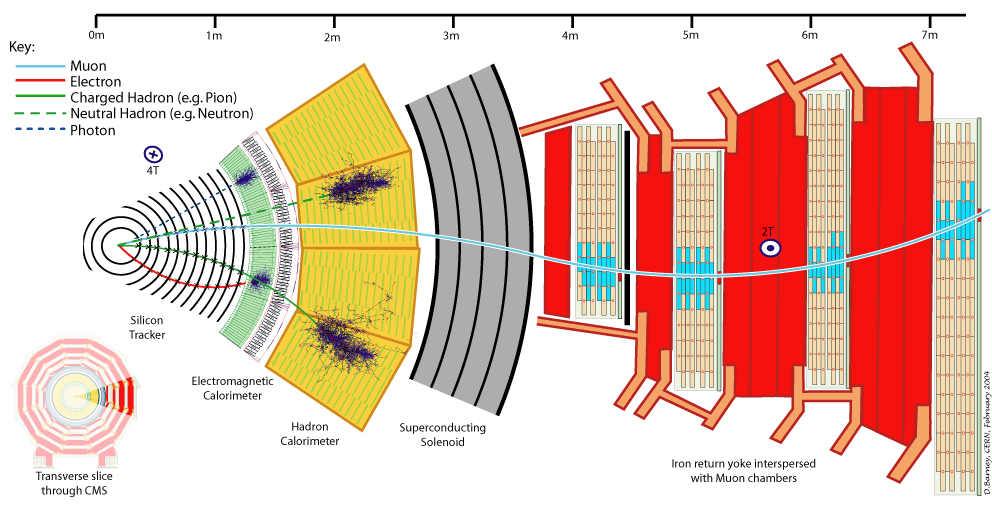
\includegraphics[width=\textwidth]{Plots/CMS/CMS_Slice}
\caption[Cross section of a slice of the CMS detector]{\label{fig:CMS_Slice} Cross section of a slice of the CMS detector in the transverse plane with different particles crossing the subsystems is shown~\cite{CMS_slice}. Only energy deposits in the most relevant subdetectors are presented for simplicity.}
\end{center}
\end{figure}
\section{Particle-Flow algorithm}
\label{sec:PF}
The \acrfull{pf} algorithm~\cite{PF}, uses the information obtained from all of the detector subsystems in the object reconstruction. The three main object collections that feed into the PF algorithm are the tracks reconstructed from hits in the tracker, energy deposits in the calorimeters, and muon candidates reconstructed from hits in the muon system.
In order to achieve object reconstruction with a high efficiency and low fake rate, iterative tracking and the calorimeter clustering methods are used in the PF algorithm.\\
The Kalman filter~\cite{KalmanFilt} method is adopted to determine single particle tracks (See Sec.~\ref{sec:PV}). Calorimeter clustering is responsible for four tasks: the detection and measurement of the energy and the direction of the stable neutral particles, their isolation from charged hadron energy deposits, reconstruction and identification of electrons and all corresponding Bremsstrahlung photons, and help the energy measurement of charged hadrons for which the track parameters were not determined accurately. After determining the single elements, a linking algorithm is used to form a block from separate elements such as tracks, muons, ECAL clusters, HCAL clusters that are possibly related to a single object. After the construction of blocks, the actual particle reconstruction and identification is performed.\\
The PF algorithm proceeds in steps according to the approximate level of ambiguity for each reconstructed objects; it starts with muons, then electrons follow, finally, it produces photons and neutral particle candidates from the remaining calorimeter clusters to arrive at a global event description.
Following to each step, already identified blocks are gradually discarded.\\
For muons, the tracks in the muon system is re-fit including the (inner) tracker track to form "global" muons if the $\chi^2$ is acceptable~\cite{muon7TeV}.
%fit to the inner tracks by requiring an acceptable $\chi^2$. These muons are also called global muons.
If the momentum of a global muon is compatible with the tracker-only measurement within three standard deviations, the muon hypothesis is kept in PF.\\
Electrons emit a bremsstrahlung radiation, which necessitates a complicated reconstruction procedure to properly associate the radiated energy with the electron candidate. The Gaussian sum filter algorithm~(GSF)~\cite{GSF} allows such recovery and is hence used in the electron reconstruction.
%which also accounts for the possible energy loses is used to perform the track fitting. 
%To ensure an optimal energy containment, all ECAL clusters in the PF block linked either to the supercluster or to one of the GSF track tangents are associated with the candidate. 
%Moreover, all ECAL clusters in the PF block linked either to the supercluster or to one of the GSF track tangents are associated with the PF candidate, To ensure an optimal energy containment.
To ensure an optimal energy containment, all ECAL clusters in the PF block, which are linked to the electron GSF track or to the supercluster, are associated with a PF electron candidate if stringent requirements on the compatibility of the track and the cluster are satisfied.\\
%based on ECAL superclusters determines the electromagnetic energy deposits that are aligned to electron candidate tracks. A particle-flow electron is formed, if the track-cluster compatibility is satisfied.\\
Having removed deposits associated with the reconstructed muons and electrons from the list of PF inputs, the neutral and charged hadrons are reconstructed from the remaining tracks. Naturally, for charged hadrons the matching calorimeter clusters are also used in this stage.\\
%Then, the individual PF objects, such as electrons, photons, muons, charged and neutral hadrons, are combined to form more complex objects: jets, or missing transverse energy.\\
%The reconstruction for photons and $\tau$-leptons will not be described since they are not used in this analysis. Detailed description of these objects can be found here \cite{Photon1}. \\
%In this analysis, the kinematic variables, which are introduced in Chapter \ref{Chap:eventSel}, are based on the reconstructed objects satisfying certain identification criteria.
After the PF algorithm, the list of particle candidates (electrons, photons, muons, charged and neutral hadrons) is fed into the higher level algorithms for example jet clustering which are discussed in the following section.\\
In this work, and from now on, all event observables are based on the list of PF candidates as produced by the PF algorithm.
%The particle candidates are reconstructed in a sequence of highest reconstruction performance to lowest, thus already identified blocks are gradually discarded for the more ambiguous object reconstructions. \\
\section{Tracks and primary vertices}
As discussed in Sec.~\ref{lhc_params}, the LHC is designed to run with a peak instantaneous luminosity of $\mathcal{L}=10^{34}\,{\rm cm^{-2}s^{-1}}$ with the proton bunches crossing at intervals of 25~ns. 
In 2016, the peak luminosity measured by the CMS experiment is 15.30~$10^{33}\,{\rm cm^{-2}s^{-1}}$ (see Fig.~\ref{fig:peaklumi_IntLumi}). Figure~\ref{fig:CMSpileup} shows the recorded luminosity with respect to the mean number of interactions per bunch crossing in the 2016 pp run at 13 TeV with $\rm <n_{vertex}>$=27. These multiple interactions are known as pileup. Due to finite time resolution of the detector, pileup is affected by the prior or later bunch crossings as well. Given these conditions, reconstructing tracks and subsequently the primary vertices is challenging~\cite{PV_1}.\\ 
%the CMS tracker is expected to be exposed by about 1000 charged particles at each bunch crossing.
%Given these conditions, the CMS tracker is expected to be traversed by about 1000 charged particles at each bunch crossing.
%Primary vertices are spread over a luminous region which is known as the beam spot. 
The purpose of primary-vertex reconstruction~\cite{PV_2} is to determine the location of all proton-proton interaction vertices in each event and the associated uncertainty on them, including the ‘signal’ vertex and any vertices from pileup collisions. It uses the available reconstructed tracks and consists of three steps.
%selection of the tracks, clustering of the tracks that appear to originate from the same interaction vertex, and fitting for the position of each vertex using its corresponding tracks.\\
The reconstruction commences with selecting a set of tracks based on some quality criteria such as the number of hits in the tracker and the impact parameter. Next, the selected tracks are clustered using a deterministic annealing (DA) algorithm~\cite{PV_3} which is finding the global minimum for a problem with many degrees of freedom. To overcome outliers that  originate from a secondary or mismeasured tracks, the DA algorithm is extended with a rejection term which acts as a cutoff against the outliers. As a result the DA algorithm becomes a one-dimensional robust adaptive multi-vertex fit~\cite{mvf}. After determining candidate vertices with the DA clustering in z, the candidates containing at least two tracks are then re-fitted using an adaptive vertex fitter~\cite{VertFit}. In the adaptive vertex fit, each track in the vertex is assigned a weight from 0 to 1. The tracks get a weight close to 1 when they are consistent with the position of the reconstructed vertex. The number of degrees of freedom:
\begin{equation}
    n_{\rm dof} = -3 + 2 \sum\limits_{i=1}^{\# tracks} w_i ,
\end{equation}
where $w_i$ is the weight for the $i$th track which is associated to a vertex. As a result, the value of $n_{\rm dof}$ is correlated with the number of tracks arising from the interaction region. Therefore, this can be also used to select true proton-proton interactions.\\
Finally, the number of good primary vertices includes vertices consistent with the luminous region (where the collisions happen),which is also known as beam spot, and with a $n_{\rm dof}\geq4$, corresponding to a minimum of four tracks.\\
%according to their z-coordinate. A vertex fit \cite{VertFit} is then applied on the clusters that more than 1cm apart and contain at least two tracks. 
The primary vertex of interest is chosen to be the vertex with the largest sum of the squared track momenta whereas the other vertices are considered as pileup vertices. The pileup vertex reconstruction and identification efficiency is about 70\%~\cite{JME2008}.\\
In the present analysis, at least a good primary vertex is required in the event selection.
\label{sec:PV}
\begin{figure}
\begin{center}
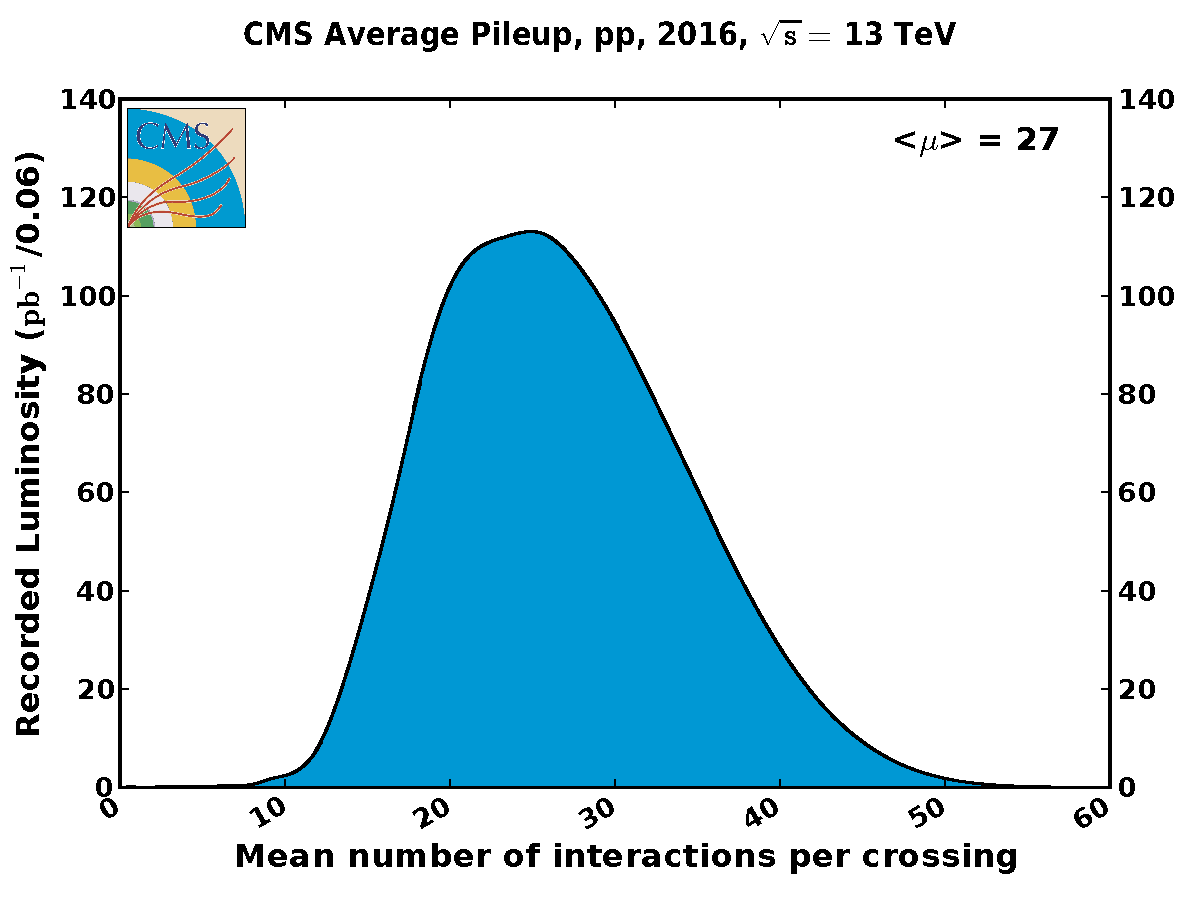
\includegraphics[width=0.8\textwidth]{Plots/CMS/pileup_pp_2016.pdf}
\caption[The mean number of interactions per bunch crossing]{\label{fig:CMSpileup} 
The recorded luminosity of data with respect to the mean number of interactions per bunch crossing in the 2016 pp run at 13~TeV~\cite{pileupCMS}. The cross section is taken to be 80~mb.}
\end{center}
\end{figure}
%%%%%%%%%%%%%%%%
%%%%%%%%%%%%%%%%
\section{Jets}
\label{sec:PFJET}
In the decays of supersymmetric gluinos, an abundance of jets is expected in the final state.\\
As already briefly mentioned in Sec.~\ref{sec:StandardModelParticleInteractions}, cascade decays of quarks and gluons lead to collimated sprays of hadrons that are reconstructed as jets. The main purpose is to reproduce the energy of the original parton prior to the shower. Jets are clustered from all PF candidates using the anti-k$_T$ algorithm~\cite{antiKT}. 
%As jets of particles propagate through the CMS detector, according to their particle content, they leave traces in all of the sub-detectors. To form a reconstructed jet, all these detector responses are combined using various jet algorithms.  
%In CMS there are two types of jet clustering algorithms in use: Cone algorithms and sequential algorithms. The first one uses a geometrical shape assumption, while the latter starts with clustering two of the closest objects together and iteratively reconstruct a closed area of objects until a truncation criterion is satisfied \cite{JET1}.\\
The algorithm starts with clustering two of the closest objects together and iteratively reconstructs a closed area of objects until a truncation criterion is satisfied.
The distance used as the termination criterion can be formulated:
\begin{eqnarray}
{d_{i,\,j} =  min\,(k^{-2}_{{\rm t},i},k^{-2}_{{\rm t},j})\frac{\Delta^2_{i,\,j}}{R^2}}\,,\\
{d_{i,\,B}} = k^{-2}_{{\rm t},i}\,,
\end{eqnarray}
where $d_{i,\,j}$ represents the distance between entities (particles, pseudojets) $i$ and $j$ with R=0.4 and $d_{i,\,B}$ is for the distance between the entity $i$ and the beam ($B$). In the formula, $\Delta^2_{i,\,j}$ is the spatial distance in $y-\phi$ plane and $k_{{\rm t},i}$ is the transverse momentum. The $d_{i,\,j}$ is calculated iteratively until it is $d_{i,\,B}$ and then i is called a jet and it is removed from the list of entities. \\
If the energy fraction of one of the components (e.g. the neutral energy fraction which is dominated by the HCAL subdetector) exceeds 99\% then the jet is rejected, because the probability of a spurious jet from detector noise is high in such cases.\\
%According to different values of $p$, which is governing the relative power of the energy versus geometrical ($\Delta_{i,\,j}$) scales, three main algorithms can be defined.\\
%The case of $p=0$ corresponds to the Cambridge/Aachen algorithm where the termination condition is described by purely geometrical distance. The $p=1$ case is called the ${\rm k_t}$ algorithm which involves the transverse momenta of the entites as well as the geometrical distance parameter. \\
%In this analysis, the anti-${\rm k_t}$ algorithm, which is the case of $p=-1$, is used to cluster the particle flow candidates into jets. For the curious readers, the anti-${\rm k_t}$ algorithm and its performance in comparison to other algorithms are explained here \cite{antiKT}.\\
%In the present search, particle flow candidates are clustered into $R = 0.4$ jets. Jets are required to be within the pseudo rapidity range of $|\eta|<$2.4 which corresponds to the tracker acceptance.\\
The measured jet energy differs from the corresponding parton energy. There are several reasons responsible for this difference such as the non-uniform detector response, non-instrumented regions and contributions from pileup. Four multiplicative correction factors are applied to the reconstructed jet to obtain the calibrated energy~\cite{JME2011}: an offset correction, a MC calibration factor, a residual calibration for the relative energy scale, a residual calibration for the absolute energy scale.
Furthermore, only jets with the calibrated transverse momentum larger than 30 GeV are selected.
%Next, the corrections, which are known as Jet-Energy Corrections can be applied to the measured energies \cite{JEC}.
%The algorithm aims to reproduce the energy of the original parton prior to the shower.
\subsection{Identification of b jets}
\label{sec:btagging}
Jets that originate from b quarks, are important to identify processes that e.g. involve top quarks. For T5qqqqWW  (see Sec.~\ref{sec:simplifiedModels}), a veto on b-tagged jets can be used to reduce backgrounds from processes involving top quarks. Inverting the veto, in turn, allows a data driven background estimation of the contributions from $\ttbar$ events (see Sec.\ref{sec:RcsTT}).
%However, in the present analysis, the targeted SUSY model T5qqqqWW, involves no top quark; therefore in the final state no jets coming from b quarks is expected. 
%In the analysis, the events including b quark tagged jets are used to perform the $\ttJets$ background estimation (see Sec.\ref{sec:RcsTT}).
\\
The identification techniques~\cite{btagging,btagging2} utilize the rather long lifetime, $c\tau\simeq \rm 450 \mu m$, of the b quark which leads to the formation of a displaced vertex.\\
A variety of algorithms have been developed by CMS to select b~jets based on variables such as the impact parameters of charged-particle tracks, the properties of reconstructed decay vertices, and the presence of a lepton in the jet. Each of these algorithms results in a single discriminator value for each jet.
In this analysis, the combined secondary vertex~(CSV) algorithm, which uses both secondary-vertex and track-based information, is employed. The medium working point~(0.8484), which corresponds to a tagging efficiency of about 70\% and a misidentification rate of about 1\% according the $\pt$ and $\eta$ of the jet, is chosen.\\
The differences between the performance of the b-tagging algorithm when measured separately in data and simulation, are compensated by applying scale factors to simulated events, as described in Sec.~\ref{sec:SF}.
%To identify the b-tagged jets, naturally, the first step is to determine those secondary vertices (SV). 
%mention fake rate 
\section{Leptons}
\label{sec:PFleptons}
%Only the events with single lepton are considered; therefore lepton reconstruction and identification has a great importance. Additional requirements on the particle flow leptons are applied to ensure choosing a good quality lepton or rejecting the fake ones.\\
%In this analysis, only the leptons in the acceptance of $|\eta|<2.4$ with a transverse momentum of $\pt>$10 GeV are considered.
\subsection{Muons}
\label{sec:PFmuon}
%Muon reconstruction starts with the muon tracking before the PF algorithm.  
%Muons are the only charged particles reaching up to outer most layer of the CMS detector, the muon chambers. 
Muons are reconstructed in the pixel and silicon strip tracker~(tracker track) and in the DT, the CSC, and the RPC of the muon system (standalone-muon track)~\cite{muon7TeV}. The muon system guaranties a high purity while the inner tracker provides a precise momentum measurement. The candidate muons are further categorized into: global muon and tracker muon.\\
Each standalone-muon track is matched to a track in the inner tracker by requiring compatibility of the parameters of the two tracks. Then the matched hits from inner tracker and from standalone-muon track are combined and fit to form a global-muon track.\\
The tracker muon is obtained by requiring that each inner track with $\pt>0.5$ GeV and total momentum $p$ larger than 2.5 GeV is extrapolated to the muon system. The inner track is then called a tracker muon track if at least one muon segment is matched to the extrapolated track.\\
For tracks inside the geometrical acceptance, the overall reconstruction efficiency is 99\%. 
As briefly mentioned earlier, the Pf algorithm uses the global and the tracker muon properties to identify muons. Isolated global muon are selected including the information from
%PF algorithm first selects isolated global muons including the information from
inner tracker and calorimeter energy deposits in a $\Delta R$ cone with radius 0.3 in ($\eta$,$\phi$) plane in the muon direction. It is also required that the sum of the $\pt$ of the tracks and of the $E_{\rm T}$ of the deposits do not exceed 10\% of the muon $\pt$. This isolation criterion is sufficient to reject hadrons that are misidentified as muons. For the nonisolated global muons, the PF tight muon selection~\cite{muon7TeV} is applied.
%First, the muons are defined as good if they satisfy several CMS-wide identification criteria. 
%A candidate is selected as muon if the fraction of valid tracker hits above eighty percent. 
%Furthermore, several conditions are imposed according the segment compatibility evaluation. Segments are tracks which are found in a single station of the DT or CSC of the muon chamber. The segment compatibility is used to quantify the compatibility of a tracker-muon object with the muon hypothesis \cite{segment}. If the segment compatibility computation returns a value larger than 0.451 then the muon is selected, otherwise if it is below 0.303 the muon is rejected. For the candidates with intermediate segment compatibility further requirements are imposed: the muon is a global muon, the global fit gives a $\chi^2$ less than three, the $\chi^2$ of the matching between the tracker and muon is below twelve and the value returned by the kink finder is below twenty. \\
After PF muons have been selected, they are labeled as tight or loose muon according to the selections that are summarized in Tab.\ref{tab:muonSel}.
\renewcommand{\arraystretch}{1.5}
\begin{table}[ht]
\begin{center}
\begin{tabular}{|c|c|}\hline
\multicolumn{2}{|c|}{Muon Selection} \\\hline\hline
 Loose & Tight \\\hline
global or tracker muon & muon Id. in Tab.\ref{tab:muonId}\\\hline
$\pt\geq10$ GeV & $\pt\geq25$ GeV \\\hline
$|\eta|\leq2.4$ & $|\eta|\leq2.4$ \\\hline
%mini rel. isolation $\leq0.4$ &  mini rel. isolation $\leq0.2$ \\\hline
& sip$_{\rm 3D}\leq4.0$\\
\hline
\end{tabular}
\end{center}
\caption{List of selections for the tight and loose muon identification.}\label{tab:muonSel}
\end{table}
\renewcommand{\arraystretch}{1}

\renewcommand{\arraystretch}{1.5}
\begin{table}[ht]
\begin{center}
\resizebox{\columnwidth}{!}{
\begin{tabular}{|c|c|l|}\hline
\multicolumn{3}{|c|}{Muon identification} \\
%Definition  & Criteria \\
\hline
\hline
\multirow{3}{*}{Fraction of valid} &
\multirow{3}{*}{Segment compatibility }
 & Global muon  \\
 && Normalized global-track $\chi^2$  $\leq3$ \\
 \multirow{1}{*}{tracker hits} &
 \multirow{1}{*}{$\geq0.303$ }
  & $\chi^2$ of the matching between the tracker and\\
 \multirow{1}{*}{$\geq80\%$} &
 & Standalone muon position  $\leq12$ \\
 && Tracker kink finder  $\leq 20$ \\ \cline{2-3}
& \multicolumn{2}{c|}{or}  \\\cline{2-3}
&\multicolumn{2}{|c|}{Segment compatibility  $\geq0.451$}  \\\hline
\end{tabular}
}
\end{center}
\caption{List of selections for the muon identification.}\label{tab:muonId}
\end{table}
\renewcommand{\arraystretch}{1}
\subsection{Electrons}
\label{sec:PFelectrons}
Reconstruction of electrons is based on momentum information obtained from the tracker detector and energy measurements of the clusters in the ECAL~\cite{ELEID}.
The tracker material causes significant bremsstrahlung along the electron trajectory. Due to the CMS magnetic field, this bremsstrahlung spreads over a large volume in the azimuthal direction. Consequently, an electron looses on average of 33\% of its energy before reaching the ECAL at lower pseudorapidity regions while the energy loss can be up to 86\% when it passes through the budget material.\\
The subdetector geometries in the barrel and in the endcaps are different. Therefore dedicated algorithms are used for the clustering of the electron energy in these regions: the hybrid and multi-5x5 algorithms are used for the barrel and the endcaps respectively. The energy is measured in terms of superclusters, that are clusters of the clusters from bremsstrahlung photons.\\
The electron track reconstruction starts with seeding. To initiate the building of trajectories in the inner tracker, combined results of two algorithms is used: the ECAL-based seeding and the tracker-based seeding. In the ECAL-based seeding, the supercluster energy and position are employed to extrapolate the electron trajectory to the collision vertex. In the tracker-based seeding, pairs or triplets of hits with the vertices obtained from pixel tracks are combined to form the tracker seeds.\\
A GSF algorithm is used for electron-track that provides GSF electron candidates. The GSF algorithm is designed to follow the track curvature accounting for the bremsstrahlung loss up the ECAL surface. GSF uses the hit collection obtained with a KF algorithm. It approximates the Bethe-Heitler distribution with a sum of Gaussian distributions. \\
The charge of the electron is evaluated from the sign of the GSF track curvature. The charge misidentification rate is 1.5\% for reconstructed electrons from Z boson decays. The momentum of the electron is calculated from a weighted combination of the measurements from track parameters and from supercluster parameters. The first one is dominant for low energy candidates and the latter is dominant for high energy candidates.\\
On the reconstructed electrons, the criteria which are listed in Tab.~\ref{tab:eleSel} are applied to identify and categorize electrons as either loose or tight.
%As mentioned earlier the particle flow reconstruction of good quality electrons \cite{ELEID} is more elaborate than the muons. 
The requirements in Tab.\ref{tab:eleId} are slightly changing between the barrel and the endcaps, due to the different granularity of ECAL. Those criteria involve the shower shape quality and the cluster energy and track momentum compatibility. In addition to the list no associated photon conversion vertex is required. The loose electrons are tuned to an average of 95\% efficiency while for tight electrons it is 70\%. 
Due to the identification inefficiency in the gap region between the ECAL barrel and endcaps, the corresponding pseudorapidity region of $1.44<|\eta|<1.56$ is excluded for reconstructed electrons.\\ 
\renewcommand{\arraystretch}{1.5}
\begin{table}[ht]
\begin{center}
\begin{tabular}{|c|c|}\hline
\multicolumn{2}{|c|}{Electron Selection} \\\hline\hline
 Loose & Tight \\\hline
loose Id. in Tab.\ref{tab:eleId} & tight Id. in Tab.\ref{tab:eleId}\\\hline
$\pt\geq10$ GeV & $\pt\geq25$ GeV \\\hline
$|\eta|\leq2.4$ & $|\eta|\leq2.4$ \\\hline
%mini rel. isolation $\leq0.4$ &  mini rel. isolation $\leq0.2$ \\\hline
& sip$_{\rm 3D}\leq4.0$\\
\hline
\end{tabular}
\end{center}
\caption{List of selections for the tight and loose electron identification.}\label{tab:eleSel}
\end{table}
\renewcommand{\arraystretch}{1}
\renewcommand{\arraystretch}{1.5}
\begin{table}[ht]
\begin{center}
\resizebox{\columnwidth}{!}{
\begin{tabular}{|c|l|c|c|}\hline
Selection        & Definition & Barrel & Endcap \\
                 &            & loose/tight & loose/tight\\
\hline
\hline
$\sigma_{i\eta i\eta}$& ECAL crystal-based shower covariance in the direction of $\eta$& 0.0114/0.0101&0.0352/0.0279\\\hline
$\Delta\eta_{in}$ &Difference between the supercluster position in the ECAL & 0.0152/0.00926& 0.0113/0.00724 \\
& and the track direction at the innermost tracker position in $\eta$&&\\\hline
$\Delta\phi_{in}$ &Difference between the supercluster position in the ECAL &0.216/0.0336 &0.237/0.0918\\
 & and the track direction at the innermost tracker position in $\phi$  & &\\\hline
H/E & Ratio of energy measured in the HCAL over&0.181/0.0597&0.116/0.0615\\
& the energy mea- sured in the ECAL&&\\\hline
$|1/E \, -\,1/p |$& Absolute difference between the inverse electron energy&& \\
&measured in the ECAL and the inverse momentum &0.207/0.012&0.174/0.00999 \\
&measured in the tracker && \\\hline
$\Delta_{xy}$&Track-vertex distance in the transverse plane &0.0564/0.0111&0.222/0.0351\\\hline
$\Delta_{z}$& Track-vertex distance along the beam axis&0.472/0.0466&0.921/0.417 \\\hline
$N^{miss}_{hits}$&Number of missing hits in the electron inner layer track& $\leq2$&$\leq3/\leq1$\\\hline
\end{tabular}
}
\end{center}
\caption{List of selection criteria for the CMS electron identification.}\label{tab:eleId}
\end{table}
\renewcommand{\arraystretch}{1}

\subsection{Isolation}
In an event, naturally, electrons and muons are also produced in b- and c-quark decays. These secondary leptons are an important background for searches with leptons that originate from W boson decays. Fortunately, these secondary leptons can be distinguished with the help of the surrounding hadronic activity. The absence of such an energy flow is qualified as isolation. The absolute isolation is quantified as:
\begin{eqnarray}
{I} = {\sum_{\Delta R < R}\pt({\rm ch.\,from\,PV})\nonumber\\
+ {\rm max}\Big[0, \sum_{\Delta R < R}\pt({\rm photons})\nonumber\\
+\sum_{\Delta R < R}\pt({\rm neutral\,\,hadrons})\nonumber\\
-\frac{1}{2}\sum_{\Delta R < R}\pt({\rm ch.\,from\,PU})\Big]},
\end{eqnarray}
where $\Delta R$ defines the angular distance to the lepton trajectory at the interaction vertex. The last term is a correction to the contributions from photons and neutral hadrons for the accompanying pileup energy. The average fraction of charged and neutral pileup contributions has been determined empirically to be one-half. Then, a relative isolation for a given radius $R$, $I_{rel}$, can be defined as the ratio of absolute isolation and the lepton $\pt$.\\
In a TeV scale SUSY scenario or, more generally, in the decay of a highly boosted top quark, the decay products can be highly collimated.
In such events, the probability of an overlap of the lepton and a jet increases.\\
To mitigate this effect, a $\pt$ dependent size of the isolation cone radius was proposed in \cite{miniIso1, miniIso2}.
The main source of overlap are particles from the hadronization of the b-jet from the top quark. The cone size of the jet can be estimated as:
\begin{eqnarray}
{\Delta R_{\rm b-jet} \approx \frac{2m_{\rm mother}}{\pt_{\rm mother}}} = {\frac{2m_b}{\pt^b}\simeq \frac{10\, {\rm GeV}}{\pt^{{\rm lep}}}}.
\end{eqnarray}
Using this approximation, the following isolation cone size is defined:
\begin{eqnarray}
{R_{\rm iso}}=
    \begin{cases}
      0.2, & \pt^{\rm lep}\leq {\rm 50\,GeV} \\
      \frac{10\, {\rm GeV}}{\pt^{{\rm lep}}}, & \pt^{\rm lep}\in {\rm (50,\,200)\,GeV} \\
      0.05, & \pt^{\rm lep}\geq {\rm 200\,GeV}
    \end{cases}
\end{eqnarray}
This varying cone size criteria is large enough for identifying secondary leptons from b-quark decays and sufficiently small for avoiding possible overlap of the lepton and jets. This new isolation is also known as mini-isolation, $I_{\rm mini}$.
%is selected according to the $\pt$ of the lepton. For a lepton coming from a boosted $W$ boson, which then will have a high $\pt$, a narrower cone size is chosen. More precisely, cone radius is set to 0.05 for the leptons with $\pt\geq$200 GeV, while for the leptons have $\pt$ less than 50 GeV a larger cone radius of 0.2 is considered. For the leptons with intermediate $\pt$, con size is given by the formula: $\frac{10\,GeV}{p_{T,\,lep}} $.
For electrons, tight(loose) lepton candidates are required to have $I_{\rm mini}$ below 0.1(0.4) while for tight(loose) muon candidates $I_{\rm mini}$ required to be below 0.2(0.4).\\
The isolation efficiency is defined as:
\begin{eqnarray}
{\epsilon_{\rm Iso}} = {\frac{N({\rm passing\,\,lepton\,\,ID\,\,and\,\,isolation\,\,requirements})}{N({\rm passing\,\,lepton \,\,ID\,\,requirements})}}.
\end{eqnarray}
A comparison of the efficiency of $I_{rel}$ and $I_{\rm mini}$ criteria is given in Fig.~\ref{fig:lep_Eff} for one of the mass scenarios of T5qqqqWW model and $\ttJets$ MC samples.
Although mini-isolation is optimized in the context of searches with top quarks, it has a higher efficiency also for 0 b-tag final states as can be seen in Fig.~\ref{fig:lep_Eff} (upper).
%Although the mini-isolation is not adjusted according to the signal models without top quarks, as can be seen in the upper panel of Fig.\ref{fig:lep_Eff} clearly, it provides higher and at the same time flat efficiency as a function of lepton $\pt$.
In the lower panel of the figure, isolation efficiency in $\ttJets$ events are shown for electrons and muons. 
Finally, it can be observed that the traditional relative isolation efficiency decreases at large lepton $\pt$, as the hadronic activity around the lepton increases.
\begin{figure}
\begin{center}
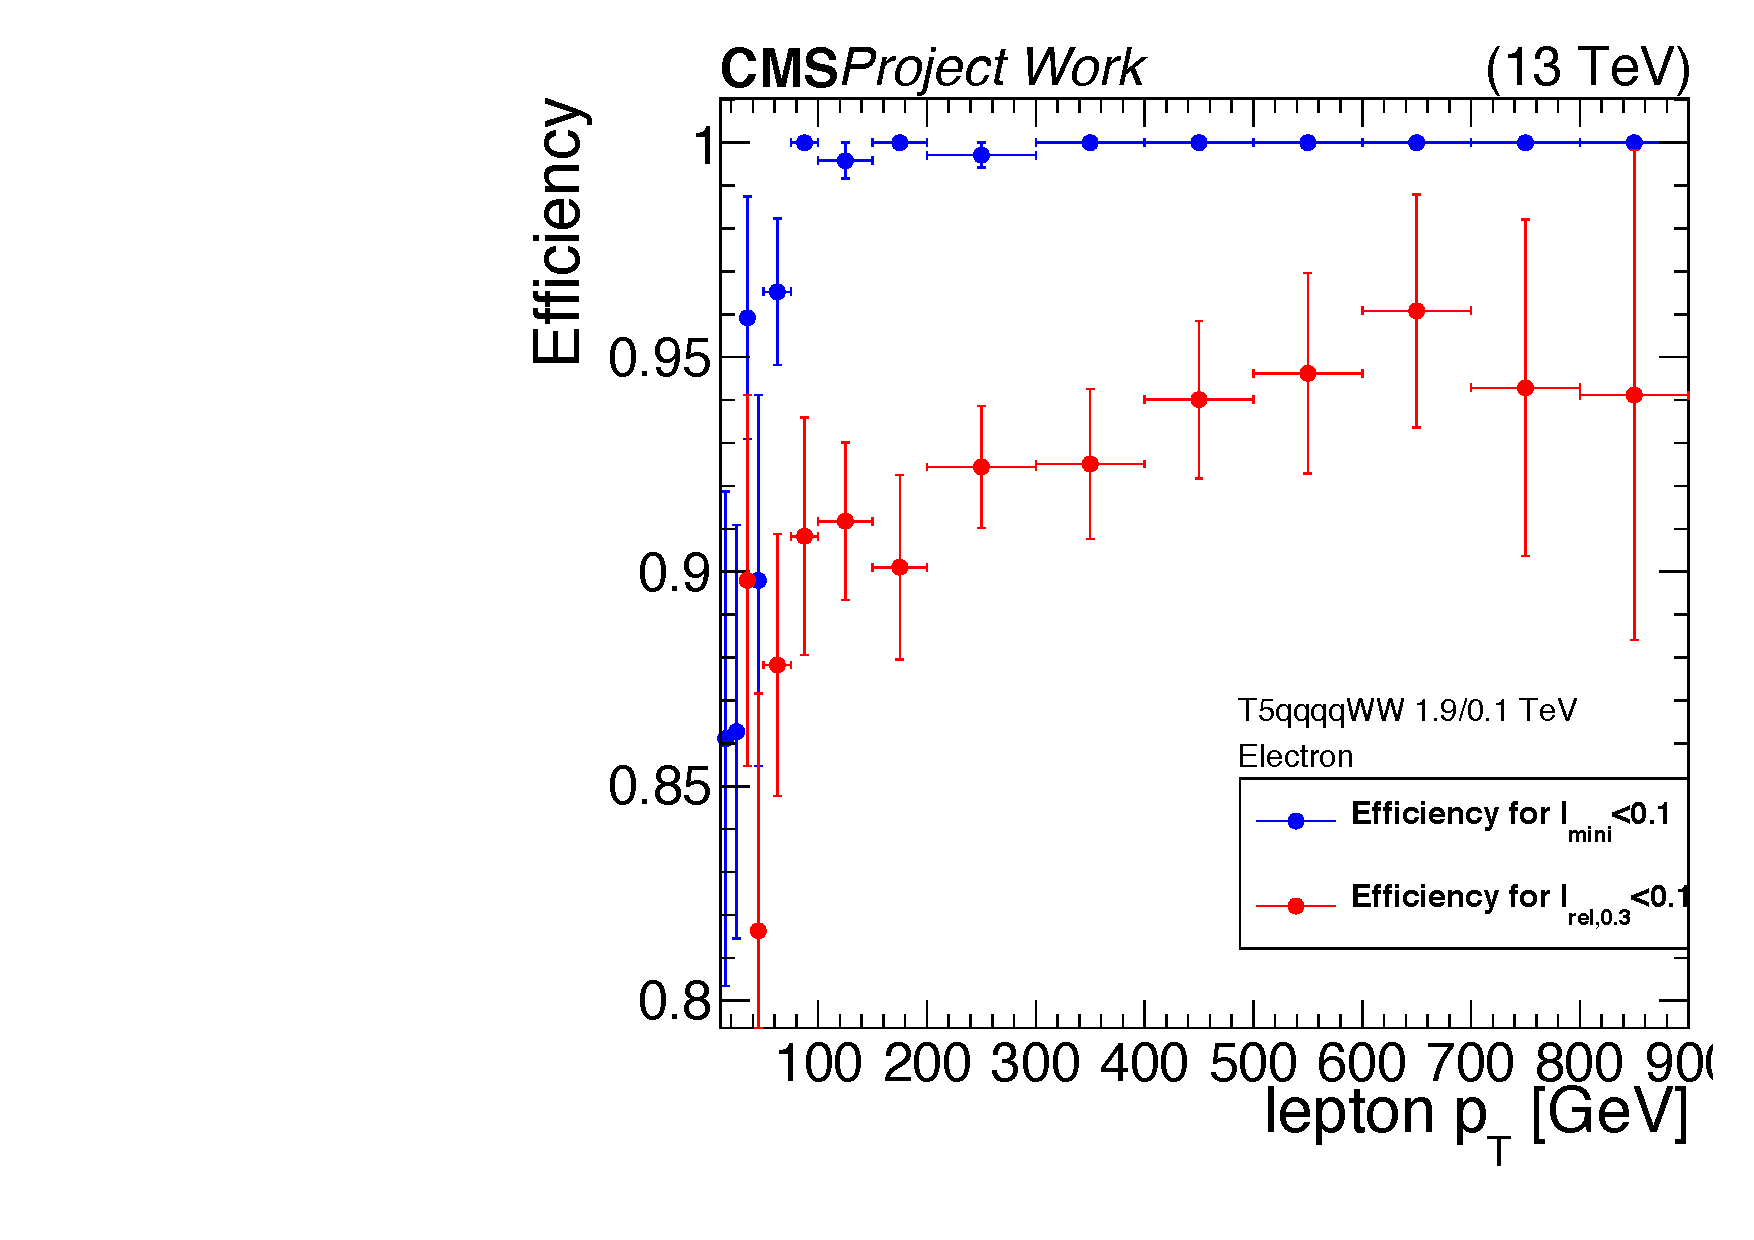
\includegraphics[width=0.45\textwidth]{PhD_Thesis_v4/Plots/lepEff/signal_EleEff.pdf}
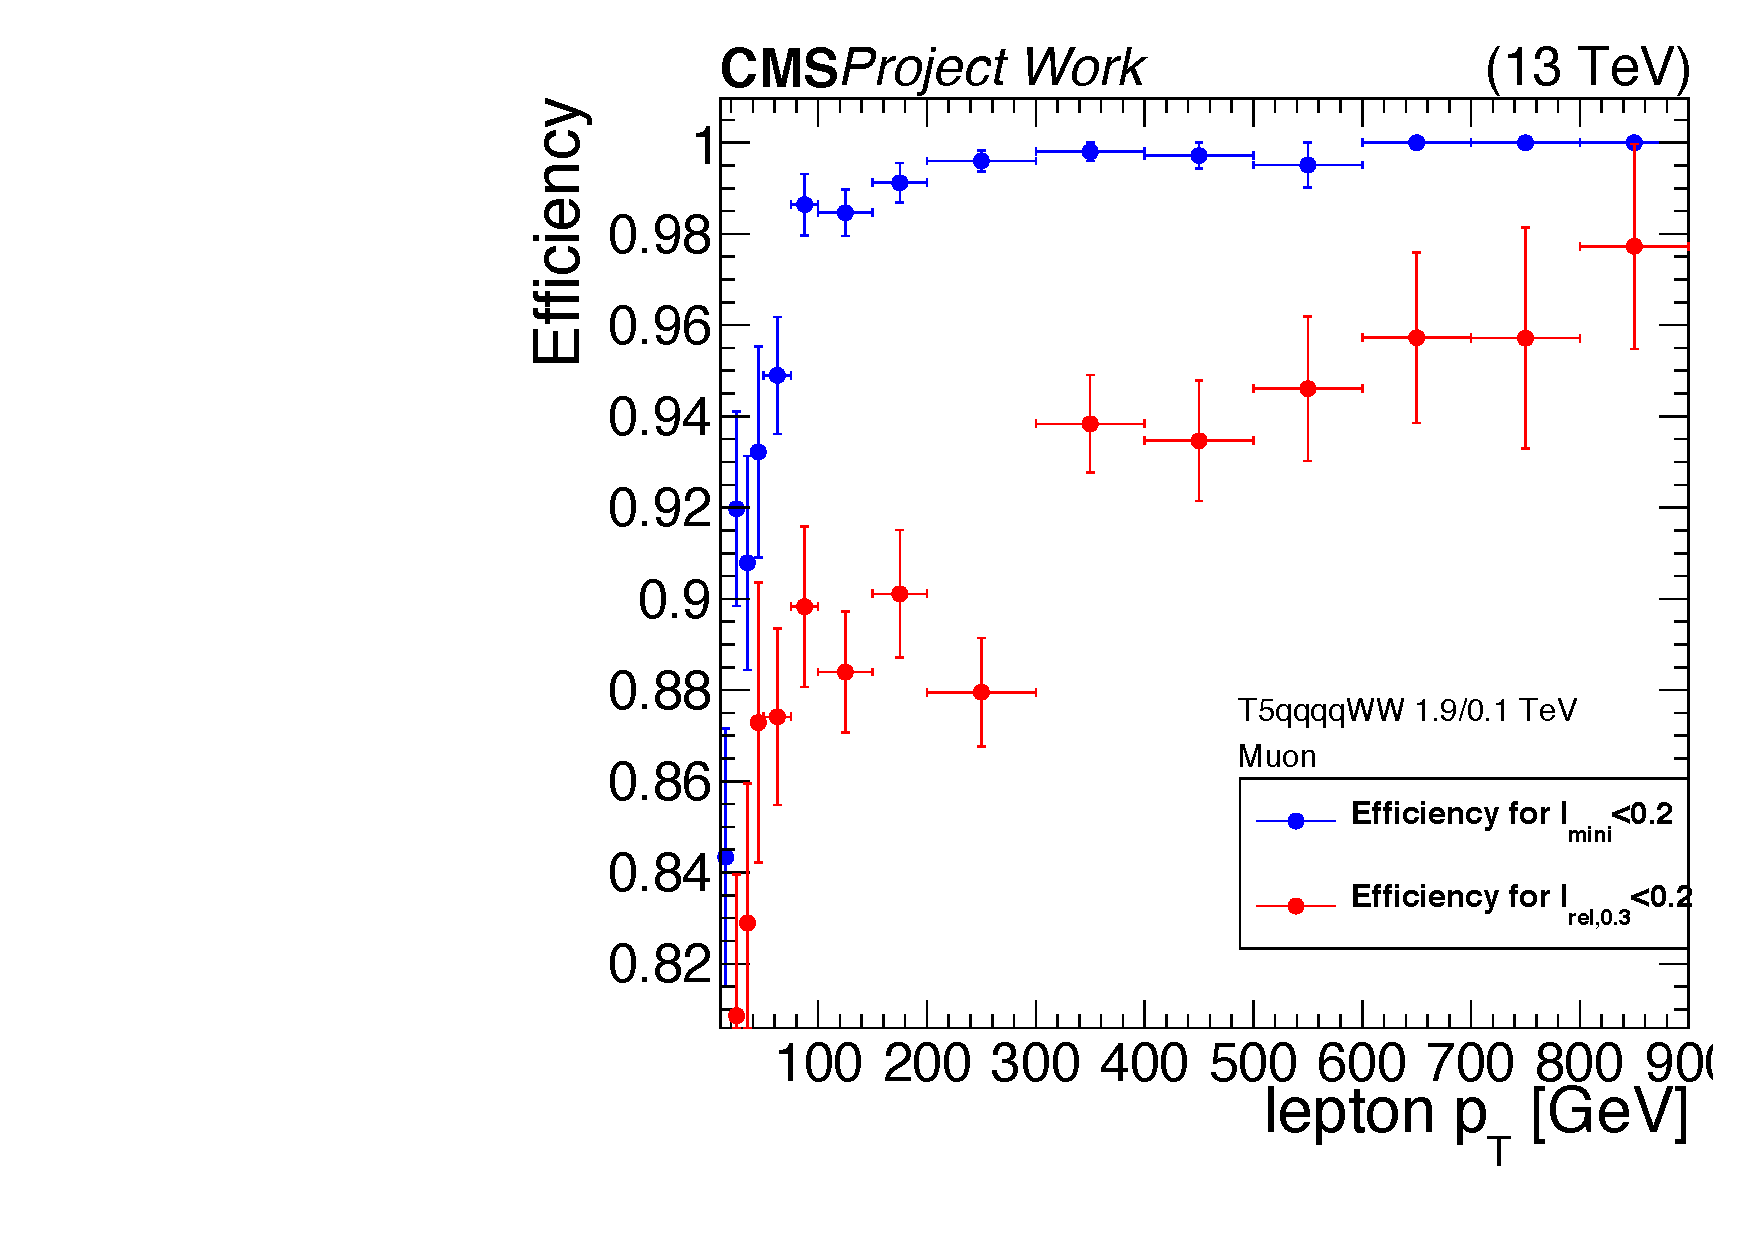
\includegraphics[width=0.45\textwidth]{PhD_Thesis_v4/Plots/lepEff/signal_MuEff.pdf}\\
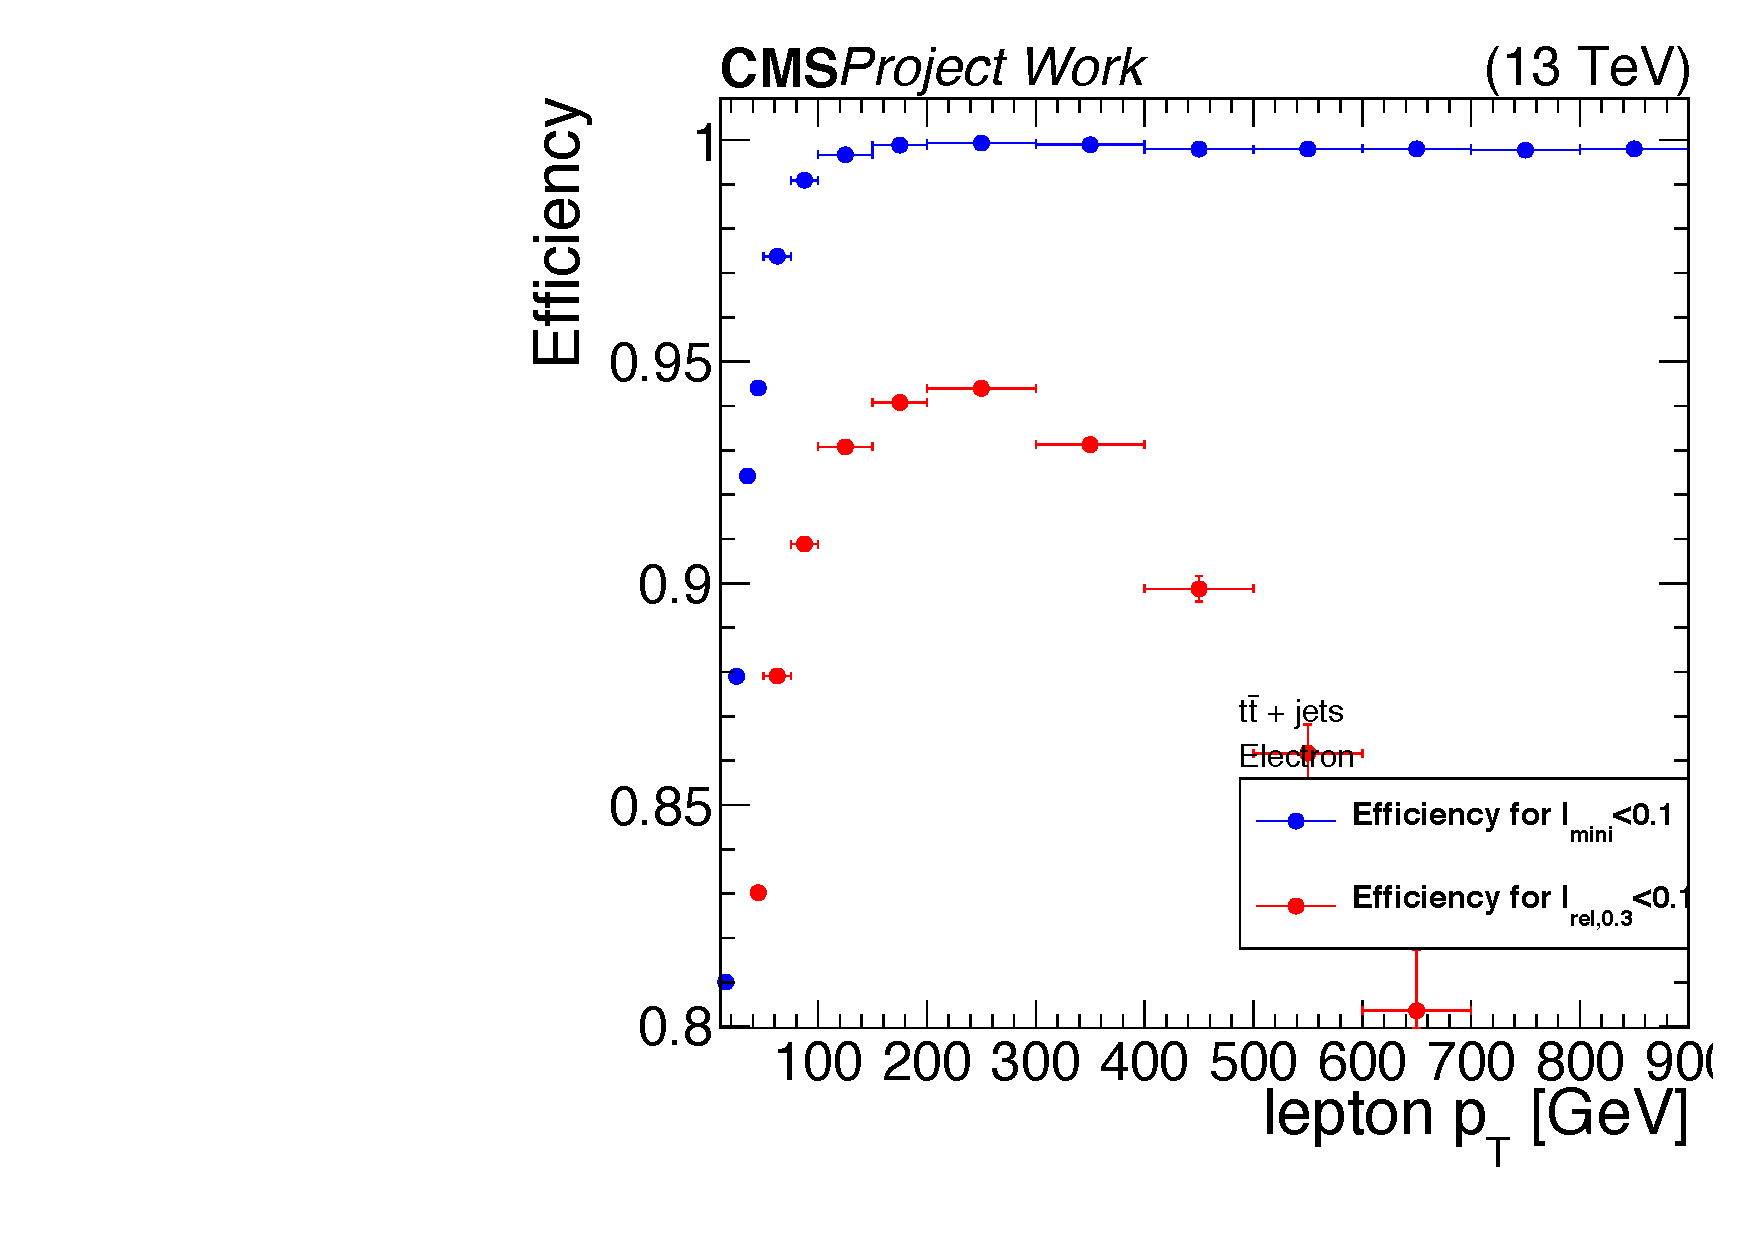
\includegraphics[width=0.45\textwidth]{PhD_Thesis_v4/Plots/lepEff/ttJets_EleEff.pdf}
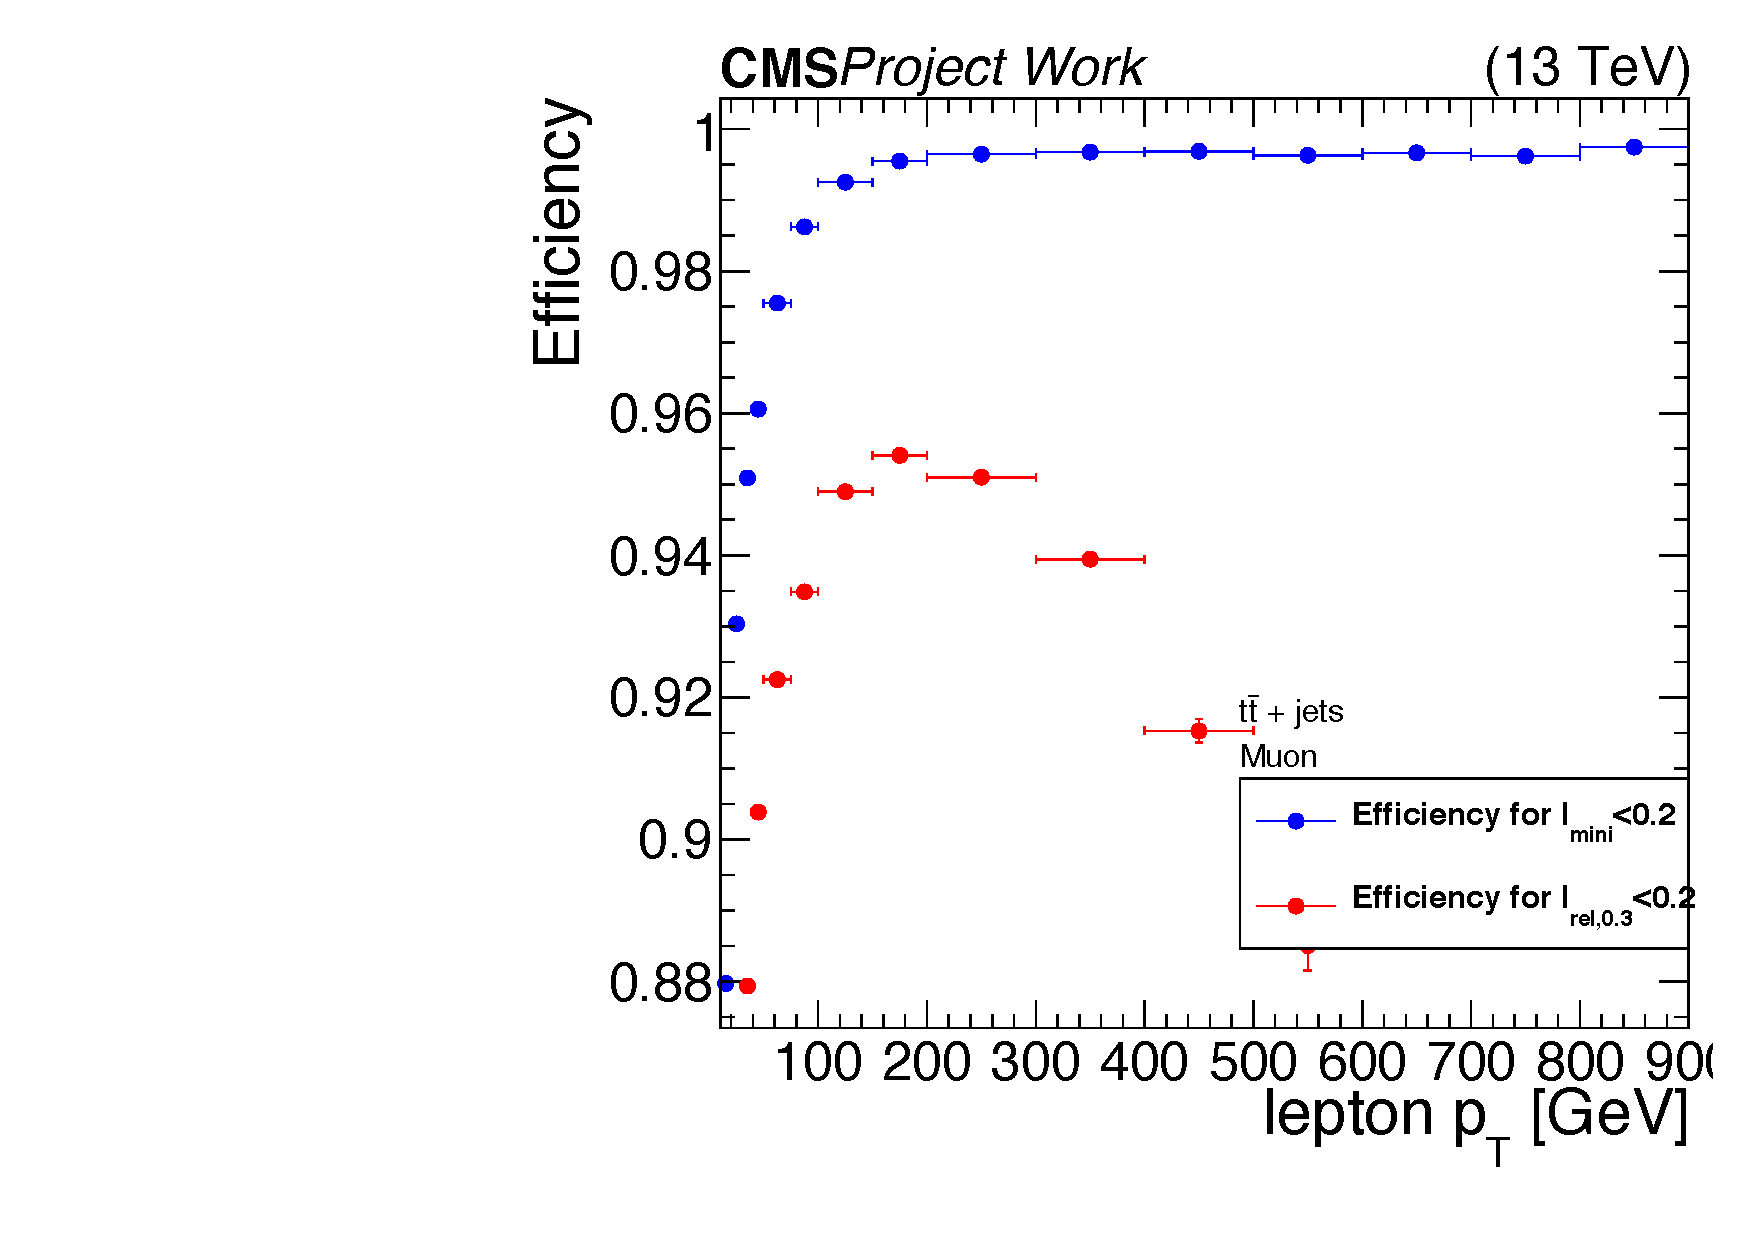
\includegraphics[width=0.45\textwidth]{PhD_Thesis_v4/Plots/lepEff/ttJets_MuEff.pdf}
\caption[Isolation efficiency comparisons]{\label{fig:lep_Eff} Isolation efficiency for simulated events for both of the mini and relative isolation is shown. The upper panel plots show T5qqqqWW (1900,100) model for electrons and muons while the lower panel plots display the efficiency in $\ttJets$ events.}
\end{center}
\end{figure}
%\newpage
\section{Missing transverse energy}
Weakly interacting massive particles, as predicted by the signal models, leave no trace in the CMS detector. Only the imbalance in transverse momentum can indirectly hint towards their existence. Missing transverse momentum~($\METvec$)~\cite{MET} is calculated from the negative transverse vector sum of all PF candidates,
% Therefore, $\METvec$ can be formulated as the negative vector sum of the transverse momentum $\pt$ of all observed particles:
 \begin{eqnarray}
 \label{Eqn:MET}
{\METvec =  -\sum_i\ptveci}\,.
\end{eqnarray}
%Otherwise, the case where $i$ stands for the calorimeter deposits is a another $\MET$ type used in CMS which is known as $Calo-\MET$. A third type of $\MET$ is an improved version of $Calo-\MET$ by corrections obtained from the tracking detector and it is called $TC-\MET$.
The $\MET$ can be mismeasured for several reasons, such as the non linearity of the calorimeter response for hadronic particles, or the minimum energy thresholds in the calorimeters. The bias in the $\MET$ measurement due to the possible reconstruction problems of PF particles can be reduced by correcting $\MET$ by the vectorial difference in the jet momenta that the jet energy corrections account for.
%propagating the jet energy corrections to the $\MET$ calculation. Additionally, $\MET$ can be biased due to pileup interactions. 
%This contribution can be subtracted as:
%\begin{eqnarray}
%{\METvec^{corr} =  %\METvec-\sum_{PU}f(\vec{v})\vec{v}}\,,
%\end{eqnarray}
%where $\vec{v}$ is the vectorial sum $\pt$ of charged particles associated with a given pileup vertex. The factor $f(\vec{v})\vec{v}$ gives the expected total $\METvec$ for each pileup interaction.\\
%Naturally, as it can be understood from the name, $PF-\MET$ is reconstructed by using the particle flow algorithm \cite{MET}. \\
%In the CMS detector, a momentum imbalance can be also originated through the various subdetector malfunctions, reconstruction effects. \\
%To be able to determine the amount of this $fake-\MET$, generally DY events where a Z boson decays to two opposite sign leptons are used because of the fact that in these kind of events the expected $real-\MET$ contribution is very low. In data, these events are selected by requiring the invariant mass of the dimuon or dielectron system is inside the Z-boson mass window, 60GeV$<M_{\ell\ell}<$120GeV.\\
In CMS, particles are produced uniformly in $\phi$, thus $\METvec$ is expected to have a flat distribution in $\phi$. However, due to the $\phi$-dependence of the detector response, imperfect alignment of different detector subsystems, and a $\sim4$~mm shift between the centre of the detector and beamline~\cite{CMS-PAS-TRK-10-003}, an asymmetry in $\phi$ is observed in data and in simulated events.\\
The observed $\phi$-asymmetry can also be viewed as a mean shift in the $\METvec$ components along the x and y detector axes. The shift shows an increasing trend in shape of a second order polynomial as a function of $\sum \pt$ of the PF candidates. To obtain the corrections, this correlation is used. First, polynomial fits are performed on $\mex$ and $\mey$ distributions as a function of $\sum \pt$ of PF candidates in various $\eta$ bins. Examples of these fits are shown in Fig. \ref{fig:phiFits}, where the dependence of $\langle\mex\rangle$ and $\langle\mey\rangle$ 
on multiplicity of PF candidates can be formulated as:
\begin{eqnarray}
\left<\mex \right> & = & c_{x_o} \cdot x + c_{x_s} \cdot x^2, \nonumber \\
\left<\mey \right> & = & c_{y_o} \cdot x + c_{y_s} \cdot x^2.
\label{eq:metPhiAsymmetryFitModel}
\end{eqnarray}
\begin{figure}[!h]
\begin{center}
\subfigure[$\mex$, sum $\pt$ of gamma in minus endcap region]{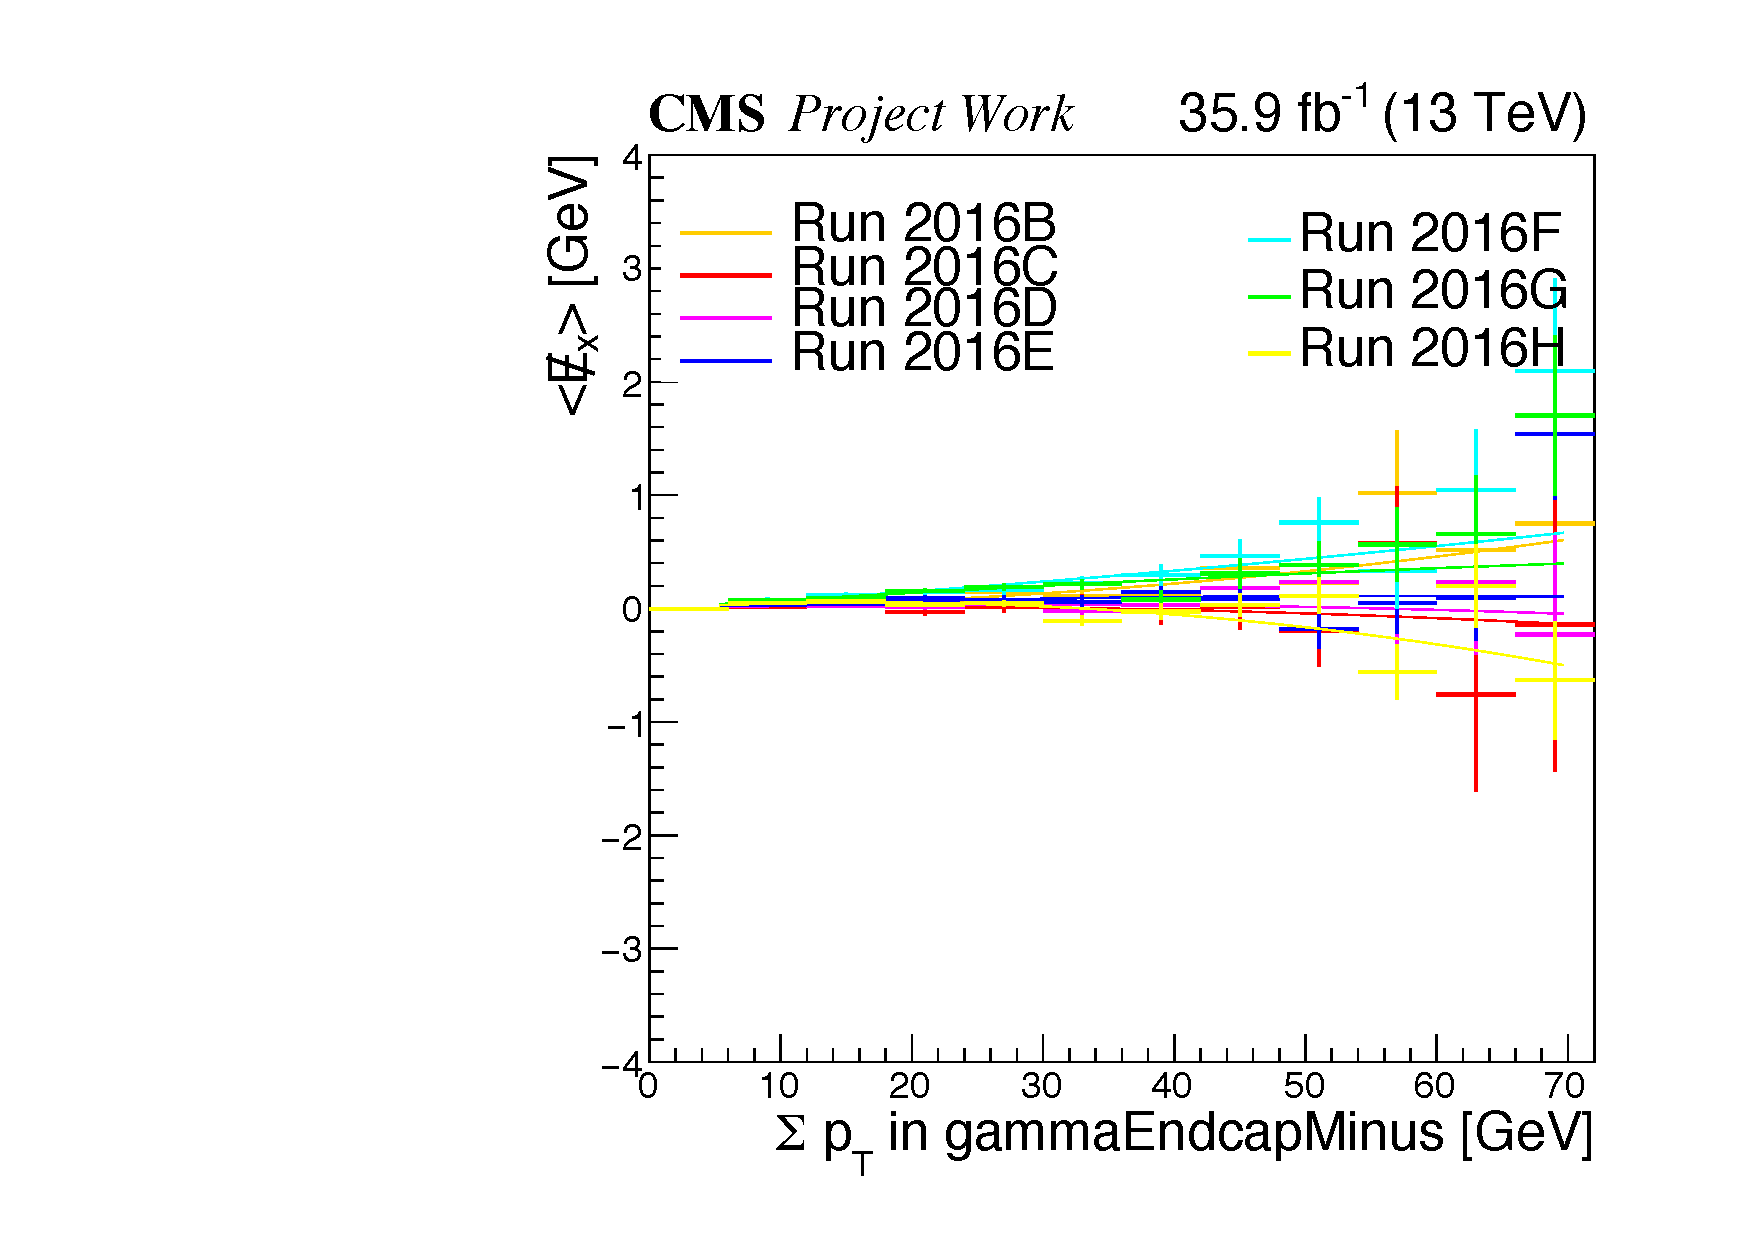
\includegraphics[width=0.45 \textwidth]{PhD_Thesis_v4/Plots/metphi/gammaEndcapMinus_Px_sumPt_.pdf}}
\subfigure[$\mey$, sum $\pt$ of gamma in minus endcap region]{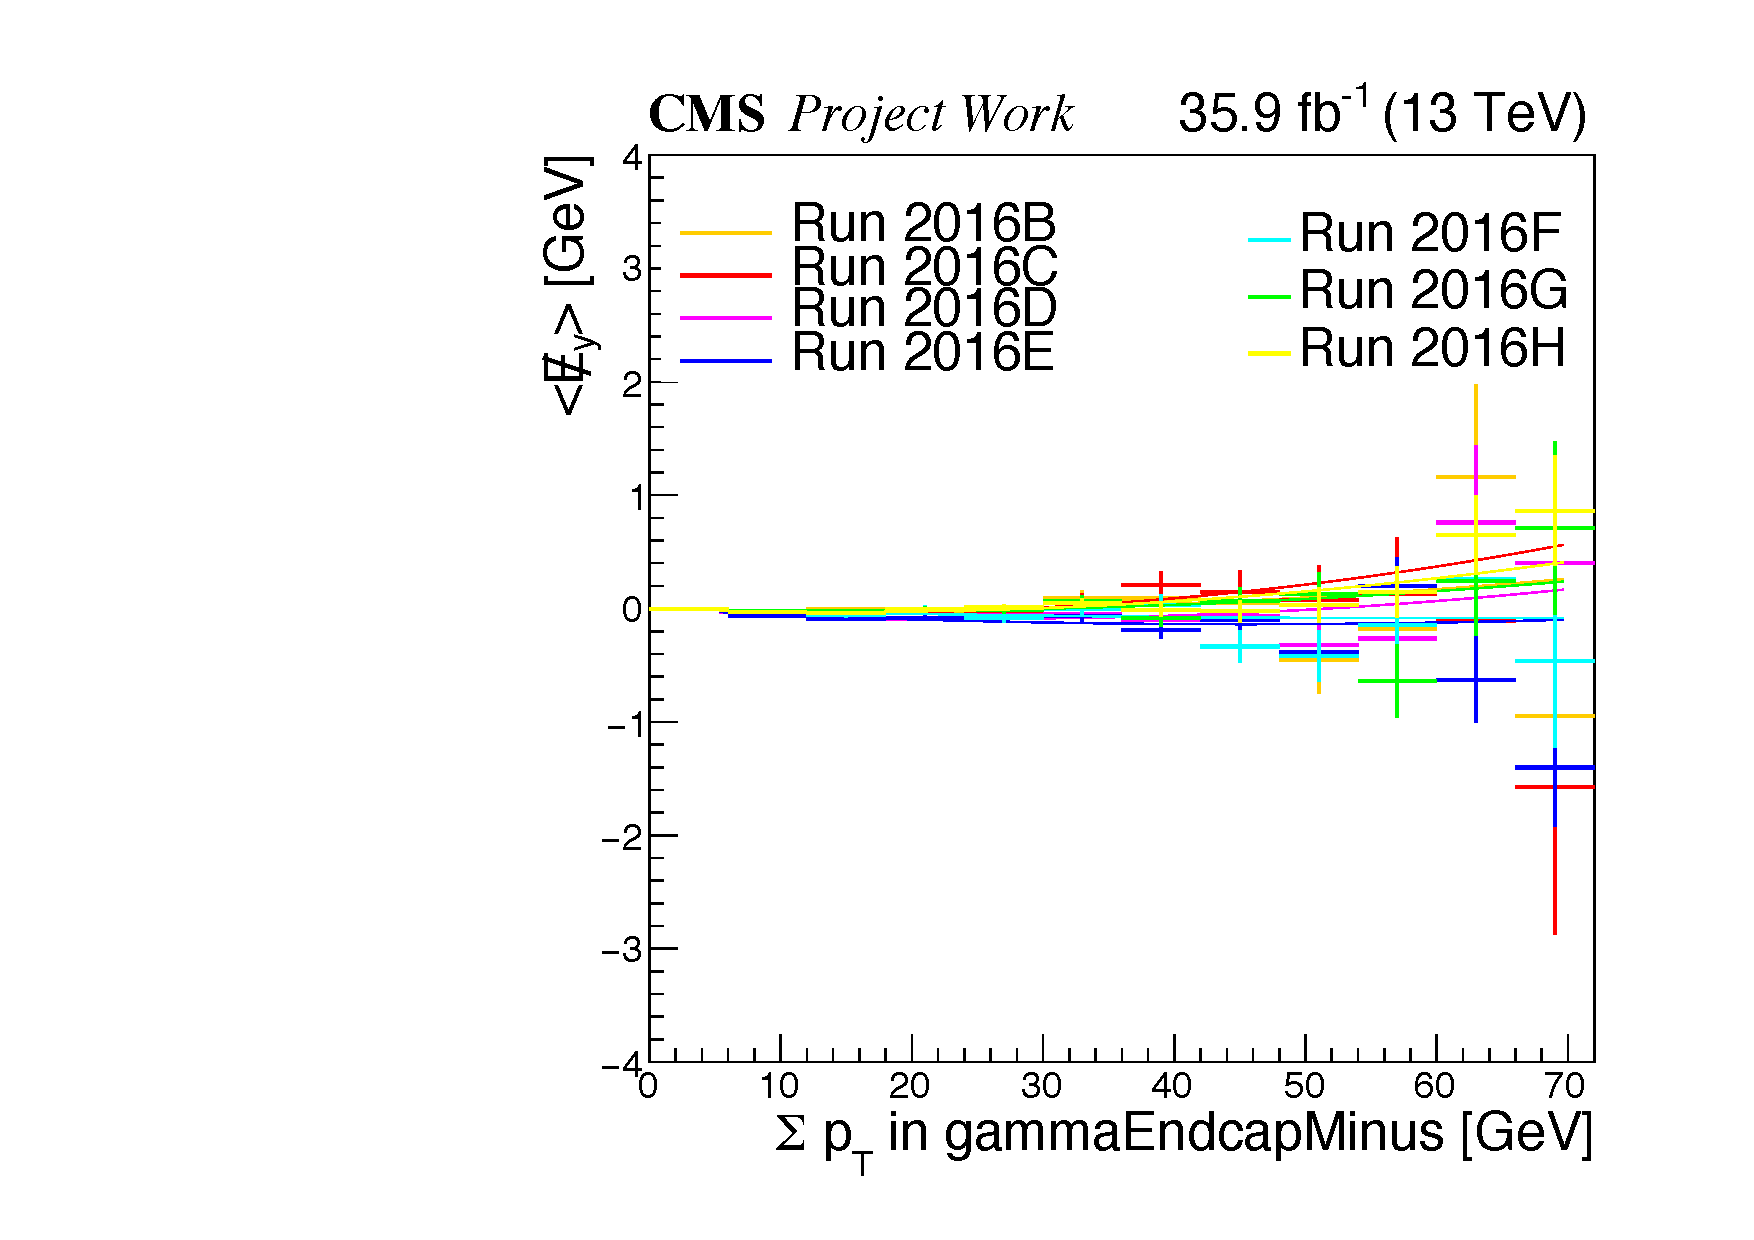
\includegraphics[width=0.45 \textwidth]{PhD_Thesis_v4/Plots/metphi/gammaEndcapMinus_Py_sumPt_.pdf}} \\
\subfigure[$\mex$, sum $\pt$ of neutral hadrons in barrel region]{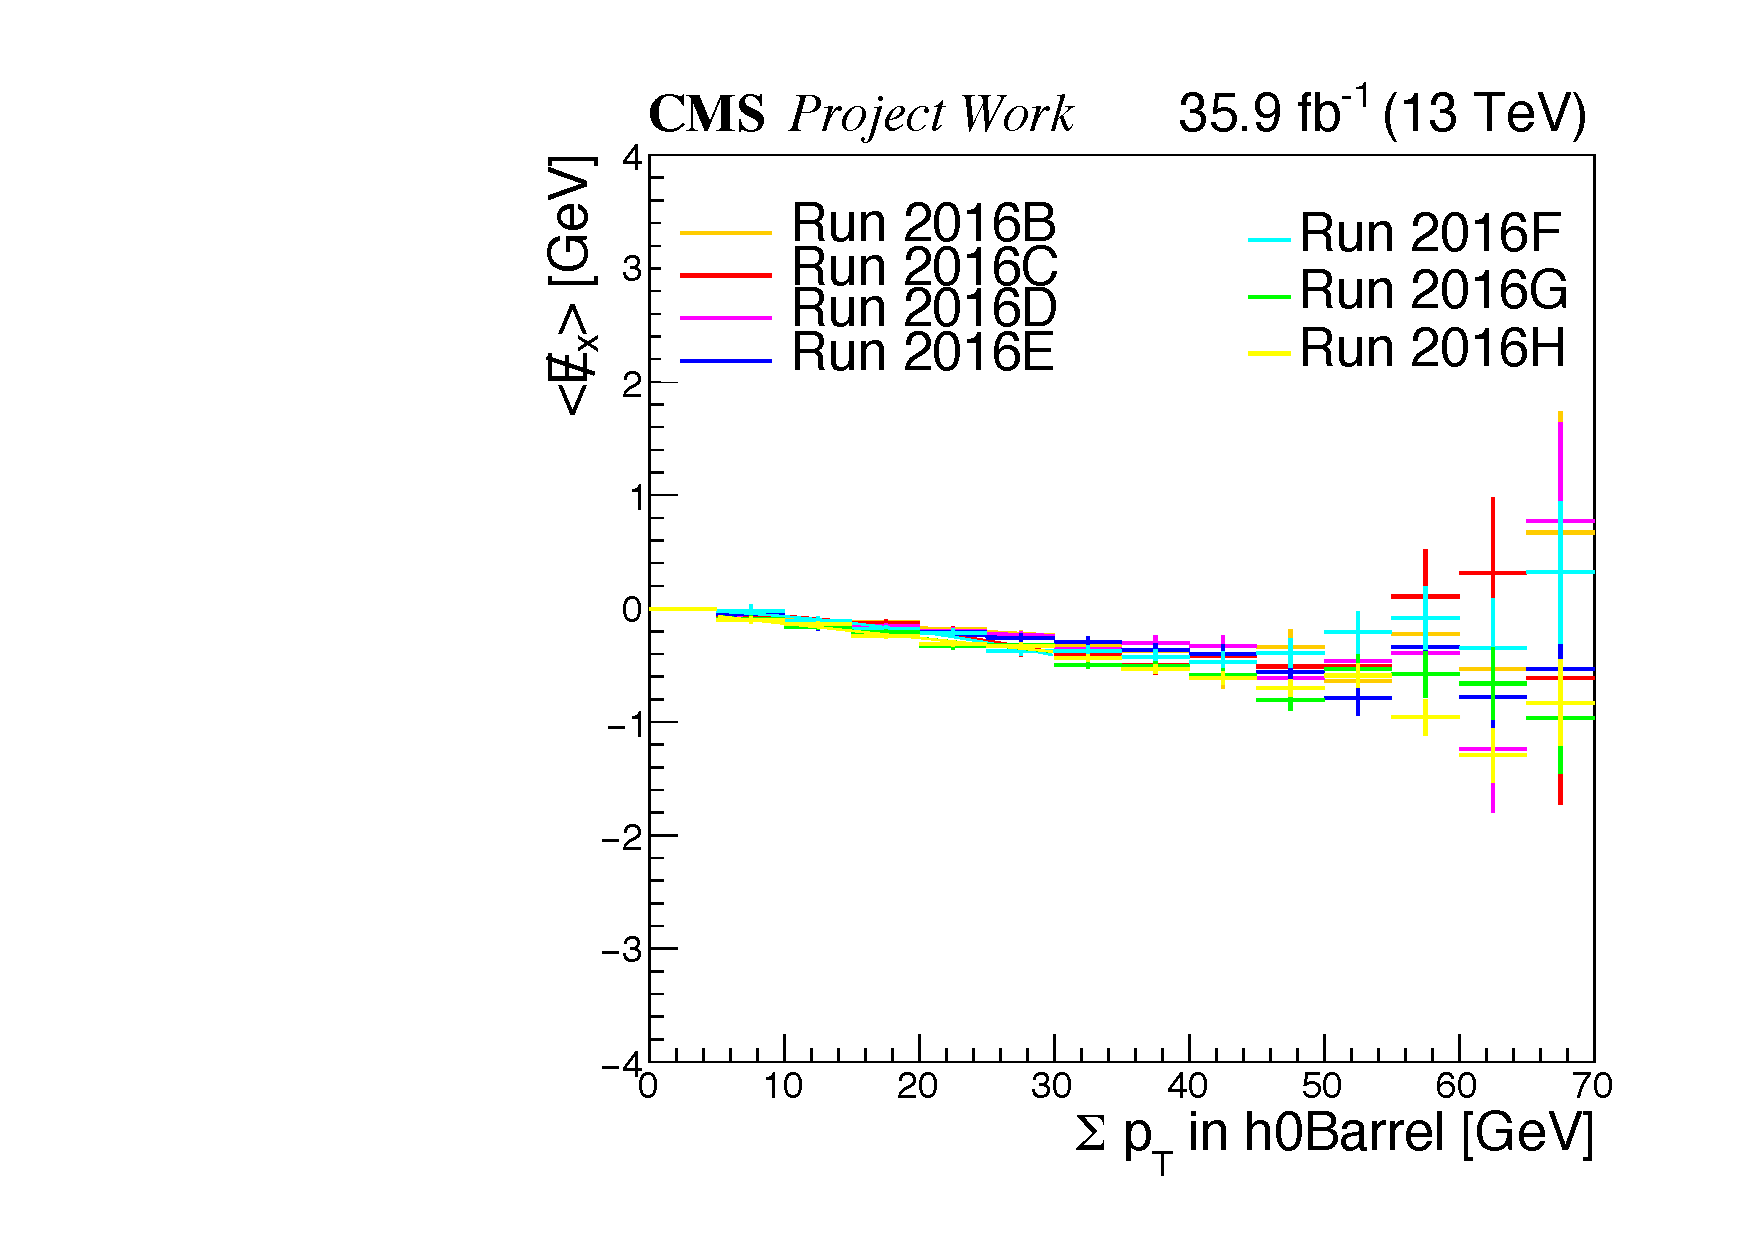
\includegraphics[width=0.45 \textwidth]{PhD_Thesis_v4/Plots/metphi/h0Barrel_Px_sumPt_.pdf}}
\subfigure[$\mey$, sum $\pt$ of neutral hadrons  in barrel region]{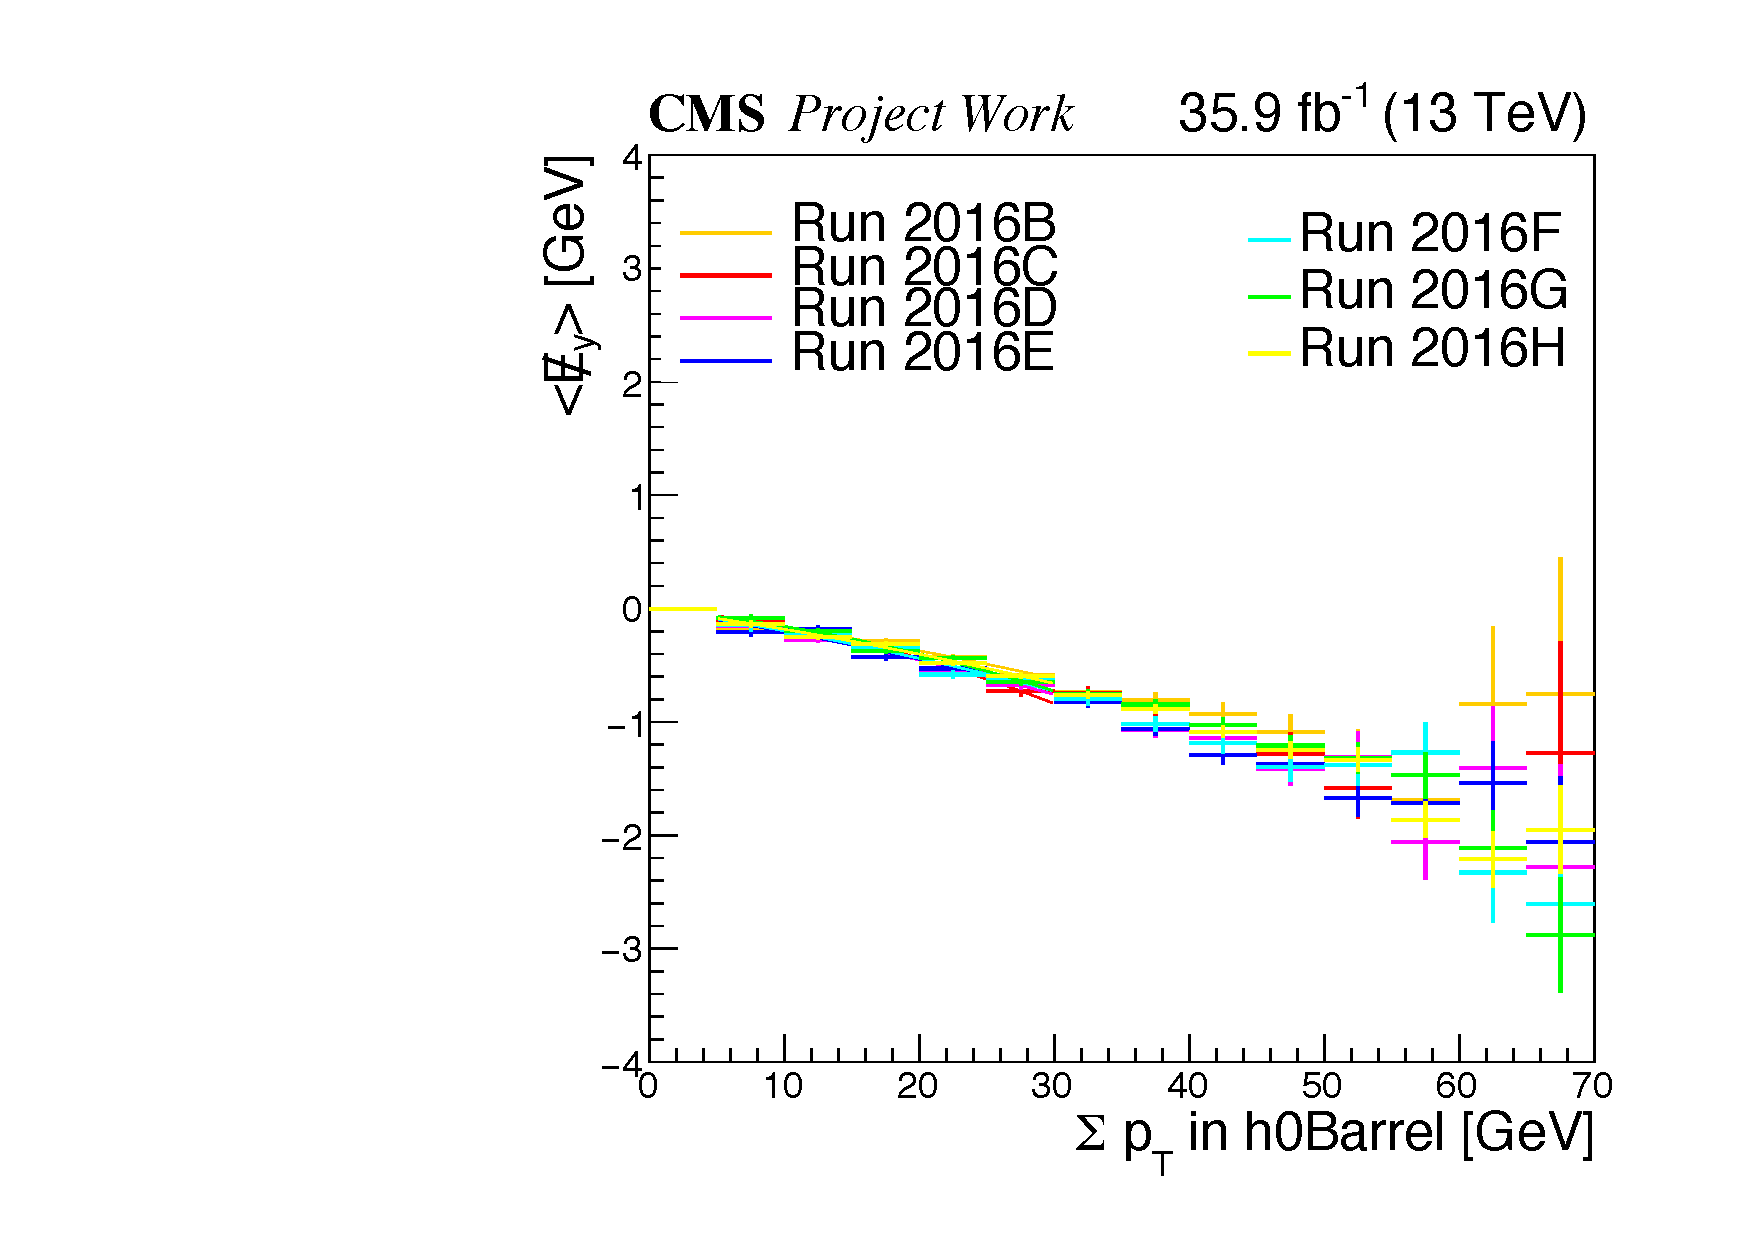
\includegraphics[width=0.45 \textwidth]{PhD_Thesis_v4/Plots/metphi/h0Barrel_Py_sumPt_.pdf}} \\
\caption{
  PF candidate multiplicity fits for \mex and \mey in different $\eta$ regions. Different colored lines represent different data taking run ranges. The Y-axis shows the average value of the x- and y-components of missing energy while X is the sum $\pt$ of the corresponding PF candidate.
  }\label{fig:phiFits}
\end{center}
\end{figure}
After the fits are performed, the corrected $\mex$ and $\mey$ can be obtained on an event-by-event basis as:
\begin{eqnarray}
\mex^\mathrm{corr} &=&  \mex - \left<\mex \right>= \mex  -(c_{x_o} \cdot x + c_{x_s} \cdot x^2), \nonumber \\
\mey^\mathrm{corr} &=&  \mey - \left<\mey \right> = \mey -(c_{y_o} \cdot x + c_{y_s} \cdot x^2).
\end{eqnarray}
The coefficients $c_{x_0}$, $c_{x_s}$, $c_{y_0}$, and $c_{y_s}$ are determined
separately from data and simulated samples. In data, the corrections are obtained in dimuon events with the invariant mass of the dimuon system is inside the Z-boson mass window, 60GeV$<M_{\ell\ell}<$120GeV. In simulated samples, the corrections are obtained by using DY events where a $Z$ boson decays to two opposite charged leptons. In such events the expected ${\rm genuine-}\MET$ contribution is very low, thus they provide a very good environment to measure $\MET$ mismodelings. The validation of the procedure is performed by using $\ttJets$ and $\wJets$ simulated samples. 
Figure~\ref{fig:metphiCorr} shows $\MET$ before and after the correction for simulated events. It is evident that there is no significant change to the spectrum while $\MET_{\phi}$ is properly corrected.
\begin{figure}[!h]
\begin{center}
\subfigure[$\MET\,\,\phi$]{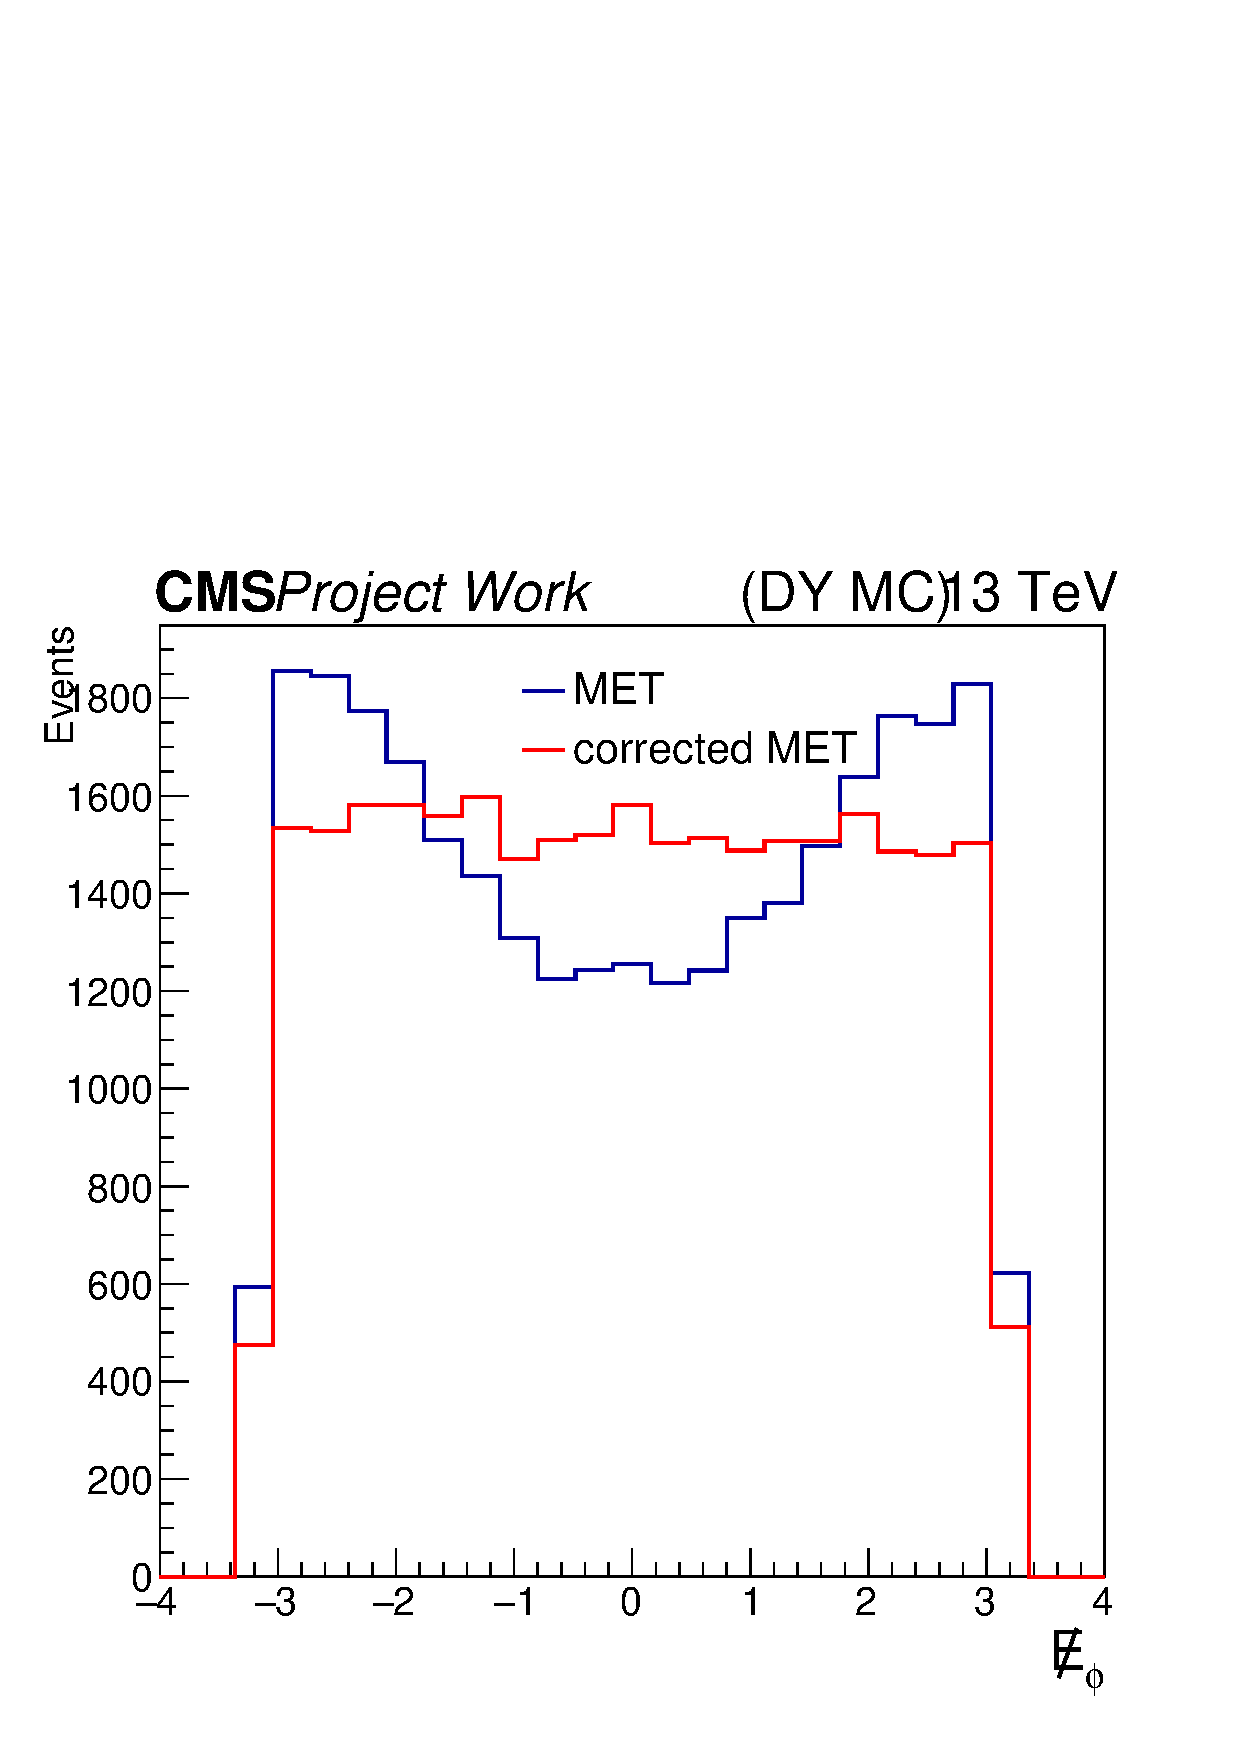
\includegraphics[width=0.5\textwidth]{PhD_Thesis_v4/Plots/metphi/DY_Comp_For_thesis.pdf}}
\subfigure[$\MET\,\,\pt$]{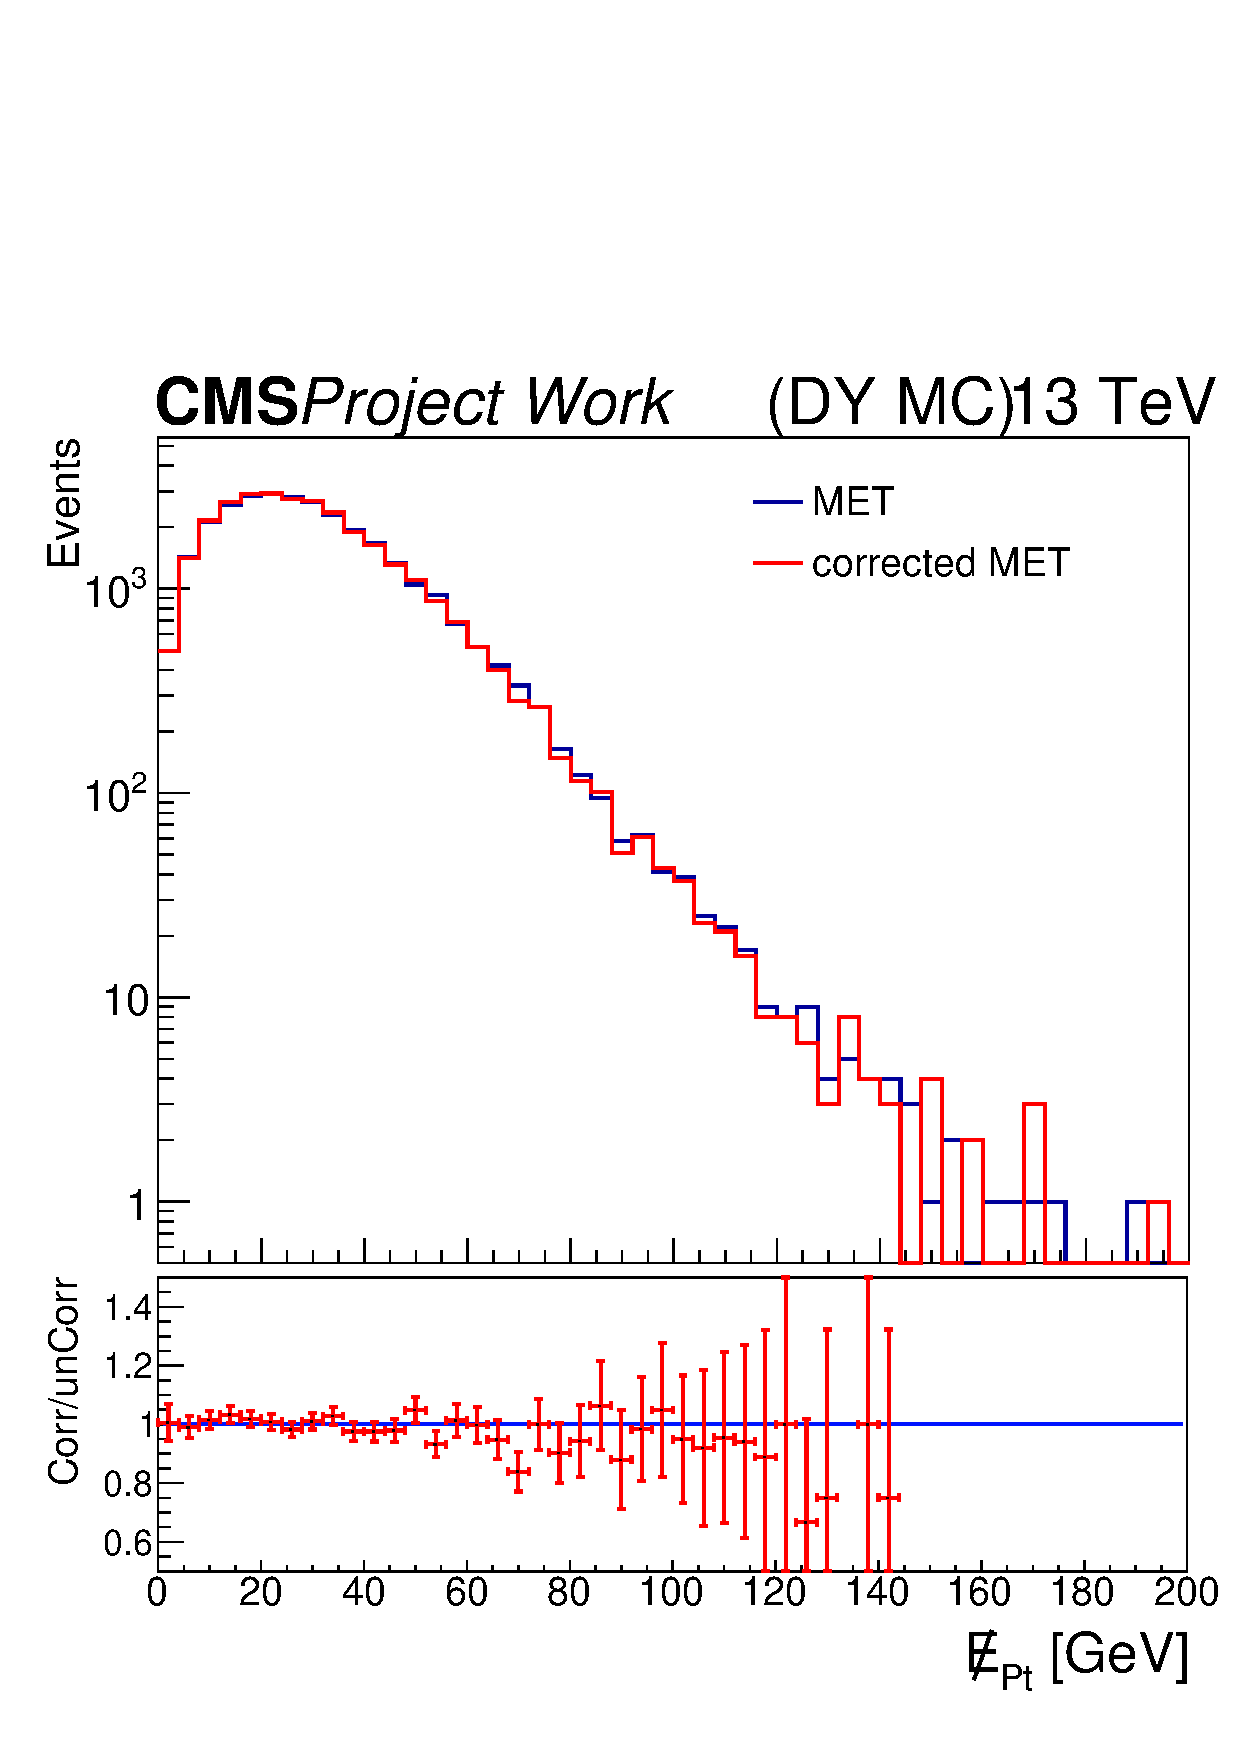
\includegraphics[width=0.45\textwidth]{PhD_Thesis_v4/Plots/metphi/DY_Comp_PT_For_thesis.pdf}}\\
\caption{
  $\MET$ $\phi$(left) and $\pt$(right) distributions before(blue) and after(red) corrections in simulated Drell-Yan events.  
  }\label{fig:metphiCorr}
\end{center}
\end{figure}
%\newpage

\chapter{Event Selection:\\Baseline and Search regions}
\label{Chap:eventSel}
\minitoc
\section{SUSY signature}
\label{signalDef}
In this thesis, as mentioned in section \ref{sec:simplifiedModels},  a search for SUSY is performed in the context of the simplified model T5qqqqWW (see Figure \ref{fig:T5qqqqWW})\footnote{Throughout this thesis, the T5qqqqWW model is sometimes referred as the signal model.}. In this model, each gluino decays to two light quarks ($c$,$s$,$u$,$d$) and an intermediate chargino, with the latter decaying to a $W$ boson and a neutralino. 
\begin{figure*}[!hb]
  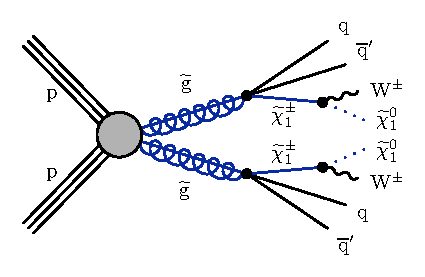
\includegraphics[width=0.5\textwidth]{Plots/feyndiagrams/T5qqqqWW.pdf}
\centering
  \caption{\label{fig:T5qqqqWW} Diagram showing the simplified model T5qqqqWW. 
  }
\end{figure*}

In the event selection, one of the $W$'s is chosen to be decaying leptonically. The choice of single lepton final states provides a cleaner event topology than the full hadronic final states while keeping the signal efficiency sufficiently high. Therefore, the visible final state includes at least six jets and one lepton (can be either electron or muon). Moreover, it is required that none of the jets are tagged as b quark to increase the probablity of selecting the events with topology T5qqqqWW. Furthermore, in such events, there is a momentum in balance originated by the neutralino and the neutrino which leave no trace in the detector. Therefore, a high missing transferse energy (MET) is also required. These selections can be further enhanced with the characteristics of individual objects such as; the transverse momentum of lepton $p_{T,\ell}$ or jets $p_{T, jets}$. 
However, only selecting events with one lepton, many jets, and high MET or using object characteristics is not enough to reveal the existence of SUSY-like events which are rare among the many SM like events with the similar final state. The $\wJets$ and $\ttJets$ events are the leading SM processes which can mimic the T5qqqqWW signature. Hence, some advanced kinematic variables need to be invented to eliminate these SM background processes. The table \ref{tab:KinVar} shows the list of variables which are used in this analysis. This list does not include the variables that are used in the identification of particle flow objects (see Sec. \ref{sec:PF}). The physics variables are categorised according to their mathematical complexity.\\
\renewcommand{\arraystretch}{1.5}
\begin{table}[ht]
\begin{center}
\begin{tabular}{|c|c|}\hline
Simple variables        & Advanced variables \\
\hline
\hline
$L_T$ , $H_T$ & $\Delta\Phi(W,\ell)$ \\
$p_{T,\ell}$ , $\eta_{\ell}$& $\MTt(\vec{p}_{\text T}^{\,\ell},\vec{p}_{\text T}^{\,t},\ptvecmiss)$  \\
$p_{T,jets\,(1,2)}$ & \\
$n_{jets}$ & \\
$n_{b-tag}$ & \\
\hline
\end{tabular}
\end{center}
\caption{List of kinematic variables}\label{tab:KinVar}
\end{table}
\renewcommand{\arraystretch}{1}
\subsection{Key variables}
\label{keyVars}
The list of simple variables consists of fundamental properties of the reconstructed physics objects, such as the transverse momentum $p_T$ of these objects, and their linear combinations.\\
%\boldmath
{\boldmath $L_{T}$} is the scalar sum of the charged lepton $p_T$ and the missing transverse momentum $E_T^{miss}$.
Given no additional source of $E_T^{miss}$, except the SM neutrino, the variable $L_T$ can be also written as: $\sqrt{p_{T(W)}^2+M_{T(W)}^2}$. The derivation of this relation is as follows:
\begin{eqnarray}
{p_{T(W)}^2} = {(p_{T(\ell)}\cdot cos\phi_{\ell} + \MET \cdot cos \phi_{\MET})^2+(p_{T(\ell)}\cdot sin\phi_{\ell} + \MET \cdot sin \phi_{\MET})^2},\nonumber \\
{M_{T(W)}^2} = {2\cdot p_{T(\ell)}\cdot\MET(1-(cos\phi_{\MET} \cdot cos\phi_{\ell} +sin\phi_{\MET}  \cdot sin\phi_{\ell} ))},\nonumber \\
{p_{T(W)}^2+M_{T(W)}^2}  = {p_{T(\ell)}^2+\MET^2+2\cdot p_{T(\ell)}\cdot\MET(cos\phi_{\MET} \cdot cos\phi_{\ell} +sin\phi_{\MET}  \cdot sin\phi_{\ell} )+2\cdot p_{T(\ell)}\cdot\MET},\nonumber \\
{(p_{T(\ell)}+\MET)^2} = {\LT^2}.
  \label{eq:LTderive}
\end{eqnarray}
For events with a single highly boosted $W$ boson ($p_{T(W)}\gg M_{T(W)}$), $L_T \sim p_{T(W)}$. This variable is also known as ``leptonic mass scale'' of the event. \\
{\boldmath $H_{T}$}  is the scalar sum of the transverse momenta of all jets above a $p_T$ threshold in the event. The major contribution to this sum is coming from transverse energy of the jets originated from the gluino decay, and it is related to the mass gap between the gluino and the chargino. This variable is reflecting the ``hadronic mass scale'' of the event. \\
{\boldmath $n_{jets}$} is the number of all jets  above a $p_T$ threshold, same as in the $H_T$ calculation, in the event.\\
{\boldmath $n_{b-tag}$} is the number of all jets tagged as coming from a b quark above a $p_T$ threshold, same as with other jets, in the event.\\
The other variables in the list such as $p_T,\ell$ or $\eta_{\ell}$ was discussed in Sec. \ref{sec:PF} regarding particle flow objects.\\
There are two advanced variables used in this analysis.\\
{\boldmath $\Delta\Phi(W,\ell)$} is the azimuthal angle between the $W$ boson and the charged lepton. In the $\wJets$ and $\ttJets$ events, the lepton comes from a leptonic decay of $W$ boson, $W\rightarrow\ell\nu$. Therefore, $\Delta\Phi(W,\ell)$ strongly related to the mass of the $W$ boson and its momentum. In SM events with high missing energy indicates that the $W$ bosons yielding the lepton and the neutrino are boosted, hence resulting in a narrow distribution in $\Delta\Phi(W,\ell)$. On the other side, in SUSY decays, the missing transverse energy comes from two neutralinos and the neutrino, which randomizes the  $\Delta\Phi(W,\ell)$, thus resulting in an even distribution in $\Delta\Phi(W,\ell)$. As a result of its features, the variable $\Delta\Phi(W,\ell)$, is the most significant variable in this analysis. The high values of $\Delta\Phi(W,\ell)$ is used as a signal region\footnote{where signal to background event counts are sufficiently large.} while the low values of $\Delta\Phi(W,\ell)$ is the control region\footnote{where signal event counts are negligible with respect to background event counts.}.\\
{\boldmath $\MTt$}  is defined as:
\begin{eqnarray}
  \MTt(\vec{p}_{\text T}^{\,\ell},\vec{p}_{\text T}^{\,t},\ptvecmiss) =
  \min\limits_{\vec{p}_{\text T}^{(1)}+\vec{p}_{\text T}^{(2)} = \ptvecmiss} \left\{
  \max \left[ \MT(\vec{p}_{\text T}^{\,\ell}, \vec{p}_{\text T}^{(1)}), 
              \MT(\vec{p}_{\text T}^{\,t},\vec{p}_{\text T}^{(2)})\right] \right\},
  \label{eq:MT2}
\end{eqnarray}
where $\MT$ is the transverse mass and the indices $t$,$\ell$ represent isolated track and the selected lepton repectively. In this analysis, this variable is used only in the baseline selection to reduce the dileptonic $\ttJets$ contribution which is more important in the signal region (high  $\Delta\Phi(W,\ell)$). 
\subsection{Signal samples}
\label{signalSamples}
The simplified model T5qqqqWW is discussed in section  \ref{sec:simplifiedModels}. This model originally includes three free parameters: the masses of the gluino $m_{\tilde{g}}$, the intermediate chargino $m_{\chipmone}$ and the neutralino $m_{\ninoone}$. To reduce the three dimension mass space the chargino mass is fixed to midway between gluino and neutralino mass. Hence, this model is investigated in the $m_{\tilde{g}}$-$m_{\ninoone}$ mass plane. For each mass point, a separate Monte Carlo sample is produced. The mass plane is shown in  Fig. \ref{fig:massplane} where the z-axis represents the total number of events generated. This scan of parameter space includes 657 mass points and it requires more computational power than usual SM process production therefore fastsim is used as explained in section \ref{fastsim}. The MADGRAPHv5 event generator is used for signal events modelling. The samples are normalized to the cross section presented by the LHC SUSY Cross Section Working Group \cite{gluxsec2}.
Throughout present thesis, two mass points corresponding to different gluino and neutralino masses are used as benchmarks to study the kinematic properties of the signal. 
\\
\textbf{T5qqqqWW(1.9,0.1)} represents a point in the high mass gap region with $m_{\tilde{g}}=$ 1900 GeV and $m_{\ninoone}=$ 100 GeV. These signal events have high \HT and \LT.
\\
\textbf{T5qqqqWW(1.5,1.0)} represents a point close to the compressed region with $m_{\tilde{g}}=$ 1500 GeV and $m_{\ninoone}=$ 1000 GeV.  The compressed region is where the $m_{\tilde{g}}-m_{\ninoone}\leq2m_{W}$. These signal events have lower \HT and \LT with respect to high mass gap ones.

\begin{figure*}[!hb]
  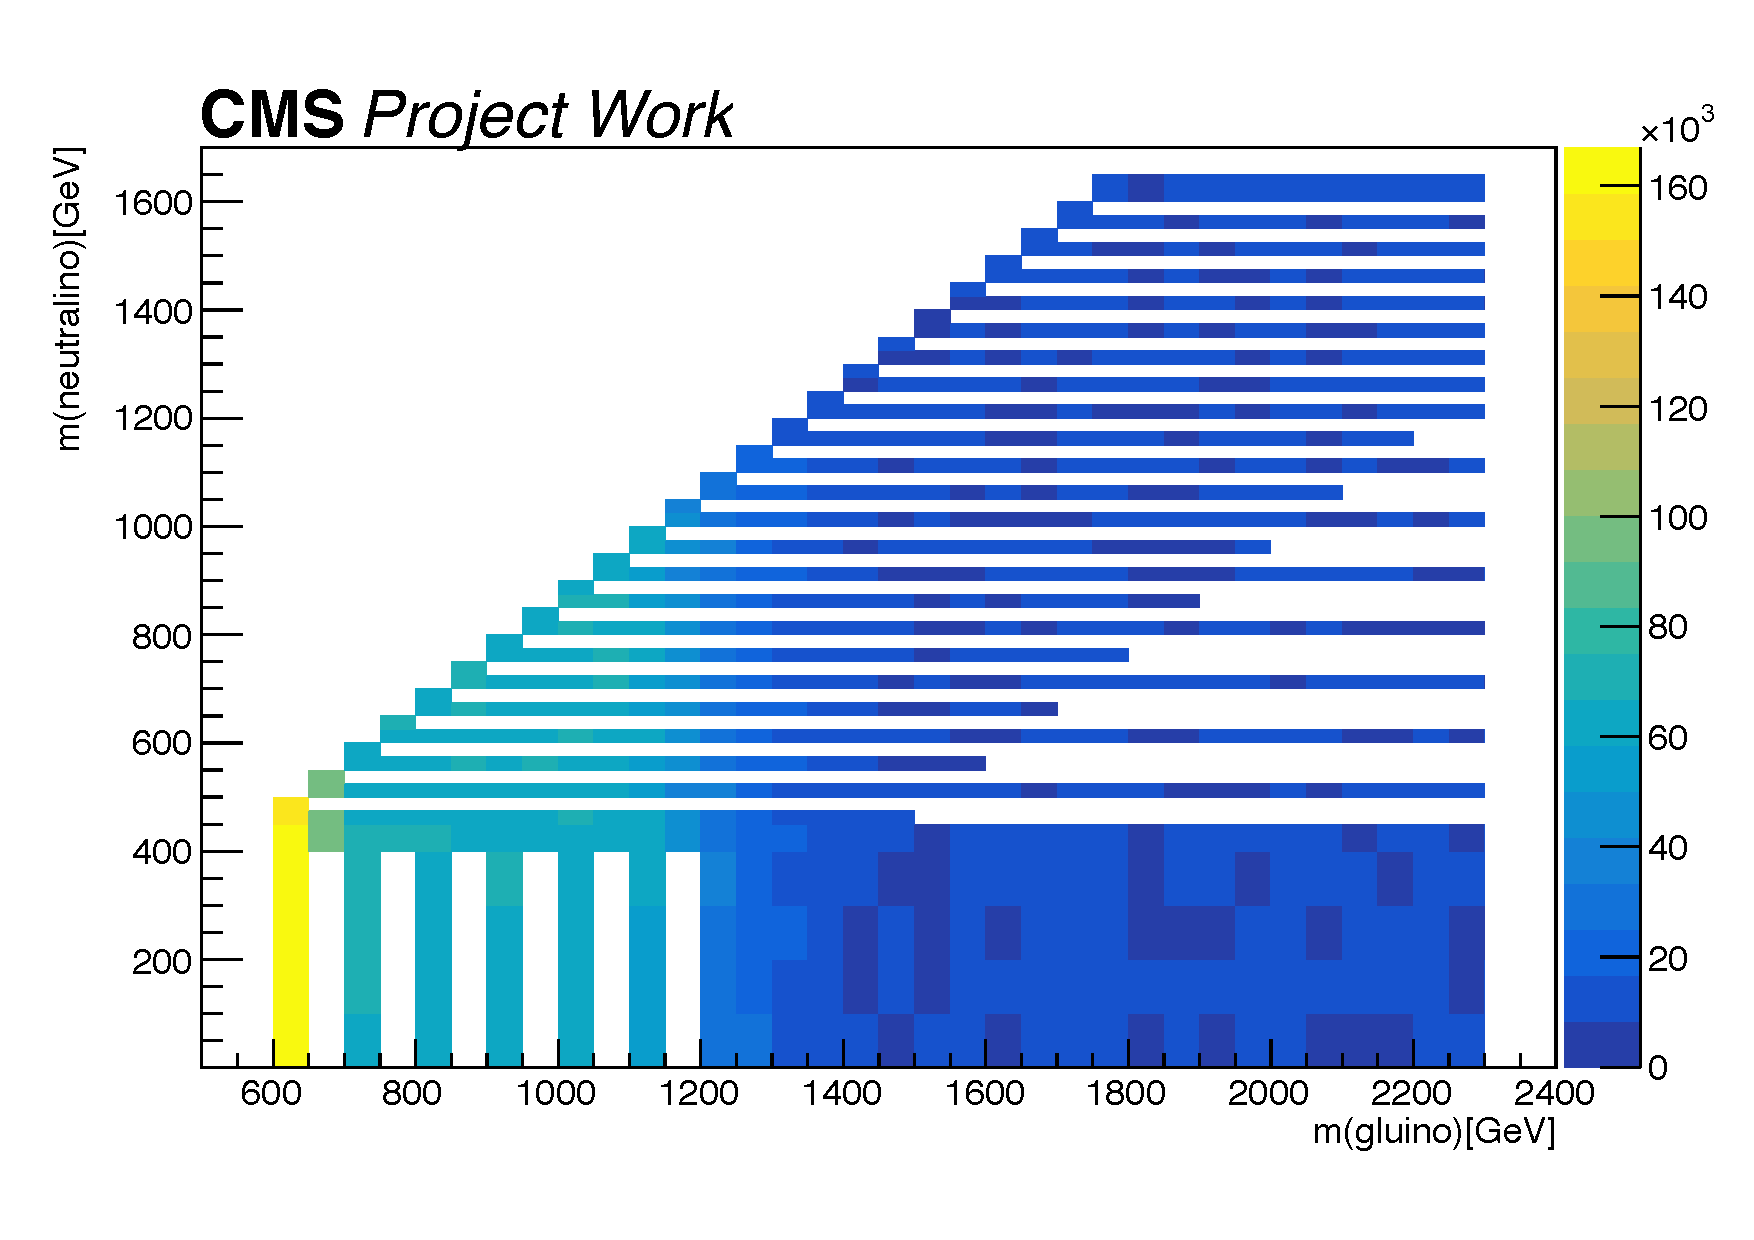
\includegraphics[width=0.7\textwidth]{Plots/signals/signal_scan.pdf}
\centering
  \caption{\label{fig:massplane} Produced signal mass points for the simplified T5qqqqWW model. 
  }
\end{figure*}

%\section{Samples}
\section{Background processes}
\label{sec:bkg_proc}
As mentioned earlier in this section the most important background processes are $\wJets$ and $\ttJets$ events. Requiring zero b-tagged jets in the event selection, $\wJets$ events becomes the main background. All of the background processes considered in this analysis are listed below. PYTHIA 8 is used for parton shower and hadronisation. \\
%\begin{aligned}
{\boldmath $\ttJets$} is generated with $\MADGRAPH$5\_\textsc{aMC@}NLOv2.2.2. To enhance the statistics the combination of $\HT$ binned samples, dedicated semi- and dilep- tonic samples is used.\\
{\boldmath $\wJets$} is generated with $\MADGRAPH$5\_\textsc{aMC@}NLOv2.2.2. $\HT$ binned samples, where $W$ decaying leptonically, are used.\\
\textbf{QCD multijets} events are produced with $\MADGRAPH$5\_\textsc{aMC@}NLOv2.2.2 in bins of $\HT$.\\
{\boldmath $\singleTop$} samples are produced with POWHEGv2.0 except the $t$ decaying leptonically with s-channel is produced with NLO $\MADGRAPH$5\_\textsc{aMC@}NLOv2.2.2. \\
\textbf{\DY} evemts are produced with $\MADGRAPH$5\_\textsc{aMC@}NLOv2.2.2 and $m_{\ell\ell}>50 GeV$ samples are used in $\HT$ bins.\\
\textbf{Di-boson} samples are produced with AMC$@$NLO except $WW$ samples are produced with powheg.\\
{\boldmath \TTVH} samples are produced with  AMC$@$NLO.\\
A list of all background MC samples with cross sections can be found in Appendix \ref{sec:Appsamples}.
%\end{aligned}
%\newpage
\subsection{Scale Factors}
\label{sec:SF}
The modeling of physics processes and the simulation of the detector responses are not perfect. Studies of the data-MC discrepancies indicate that MC needs to be corrected by some event-by-event weights, which are called scale factors. The scale factors used in this analysis are as follows:\\
\textbf{Lepton identification and reconstruction efficiency:}\\
MC samples have to be corrected according to the reconstruction and identification efficiencies of leptons.
In this work, scale factors are applied as a function of $p_{T}$ and $\eta$ of the selected lepton. They are calculated for electrons and muons separately by the e-gamma and muon physics object groups respectively\cite{leptonSF}.\\
\textbf{B-tagging efficiency:}\\
The simulated b-tagging efficiency is corrected with respect to the one in data. For each simulated event, weights corresponding to the different number of b-tagged jets values are calculated and this results in multiple weights for each event\cite{leptonSF}. This method allows reusing the events. The advantage of this method is that it provides to use full statistical power of the MC events.\\
\textbf{ISR reweighting:}\\
Since the 8 TeV Run of LHC, it is known that the $p_T$ spectrum of $\ttbar$ events are not well modeled. Therefore, an event-by-event correction is obtained using the jets from initial state radiation (ISR).
 In the present analysis, each event is corrected according to number of ISR jets. The weights can be seen in table \ref{tab:nISRweights} where the D factor is for keeping the normalization of the overall sample invariant. This D factor is calculated using an inclusive sample i.e. without the specific selections of the analysis.
 \renewcommand{\arraystretch}{1.5}
\begin{table}[htbp]
\begin{center}
\caption{Weights based on the number of ISR jets as given in Ref.~\cite{nISRweightTTbar}}
\begin{tabular}{|r|l|}
\hline
\multicolumn{1}{|l|}{nISR jet} & Normalisation weight $D_{\ttbar} = 1.071$ \\ \hline
0 &  \\ \hline
1 & $D \times (0.920 \pm 0.005 \pm 0.040)$ \\ \hline
2 & $D \times (0.821 \pm 0.006 \pm 0.090)$ \\ \hline
3 & $D \times (0.715 \pm 0.009 \pm 0.143)$ \\ \hline
4 & $D \times (0.662 \pm 0.016 \pm 0.169)$ \\ \hline
5 & $D \times (0.561 \pm 0.027 \pm 0.219)$ \\ \hline
$\geq$ 6& $D \times (0.511 \pm 0.041 \pm 0.244)$ \\ \hline
\end{tabular}
\label{tab:nISRweights}
\end{center}
\end{table}
\\
\renewcommand{\arraystretch}{1}
\textbf{Pileup:}\\
As discussed earlier in Section \ref{sec:PrimaryVert}, the number of pile-up interactions in simulated samples is generated with a prior distribution. Thus, the MC pile-up distribution may vary from the actual pile-up distribution in Data. The simulated distribution is rescaled with the Data/MC ratio in Figure \ref{fig:pileUpmine}.
\begin{figure*}[!hb]
  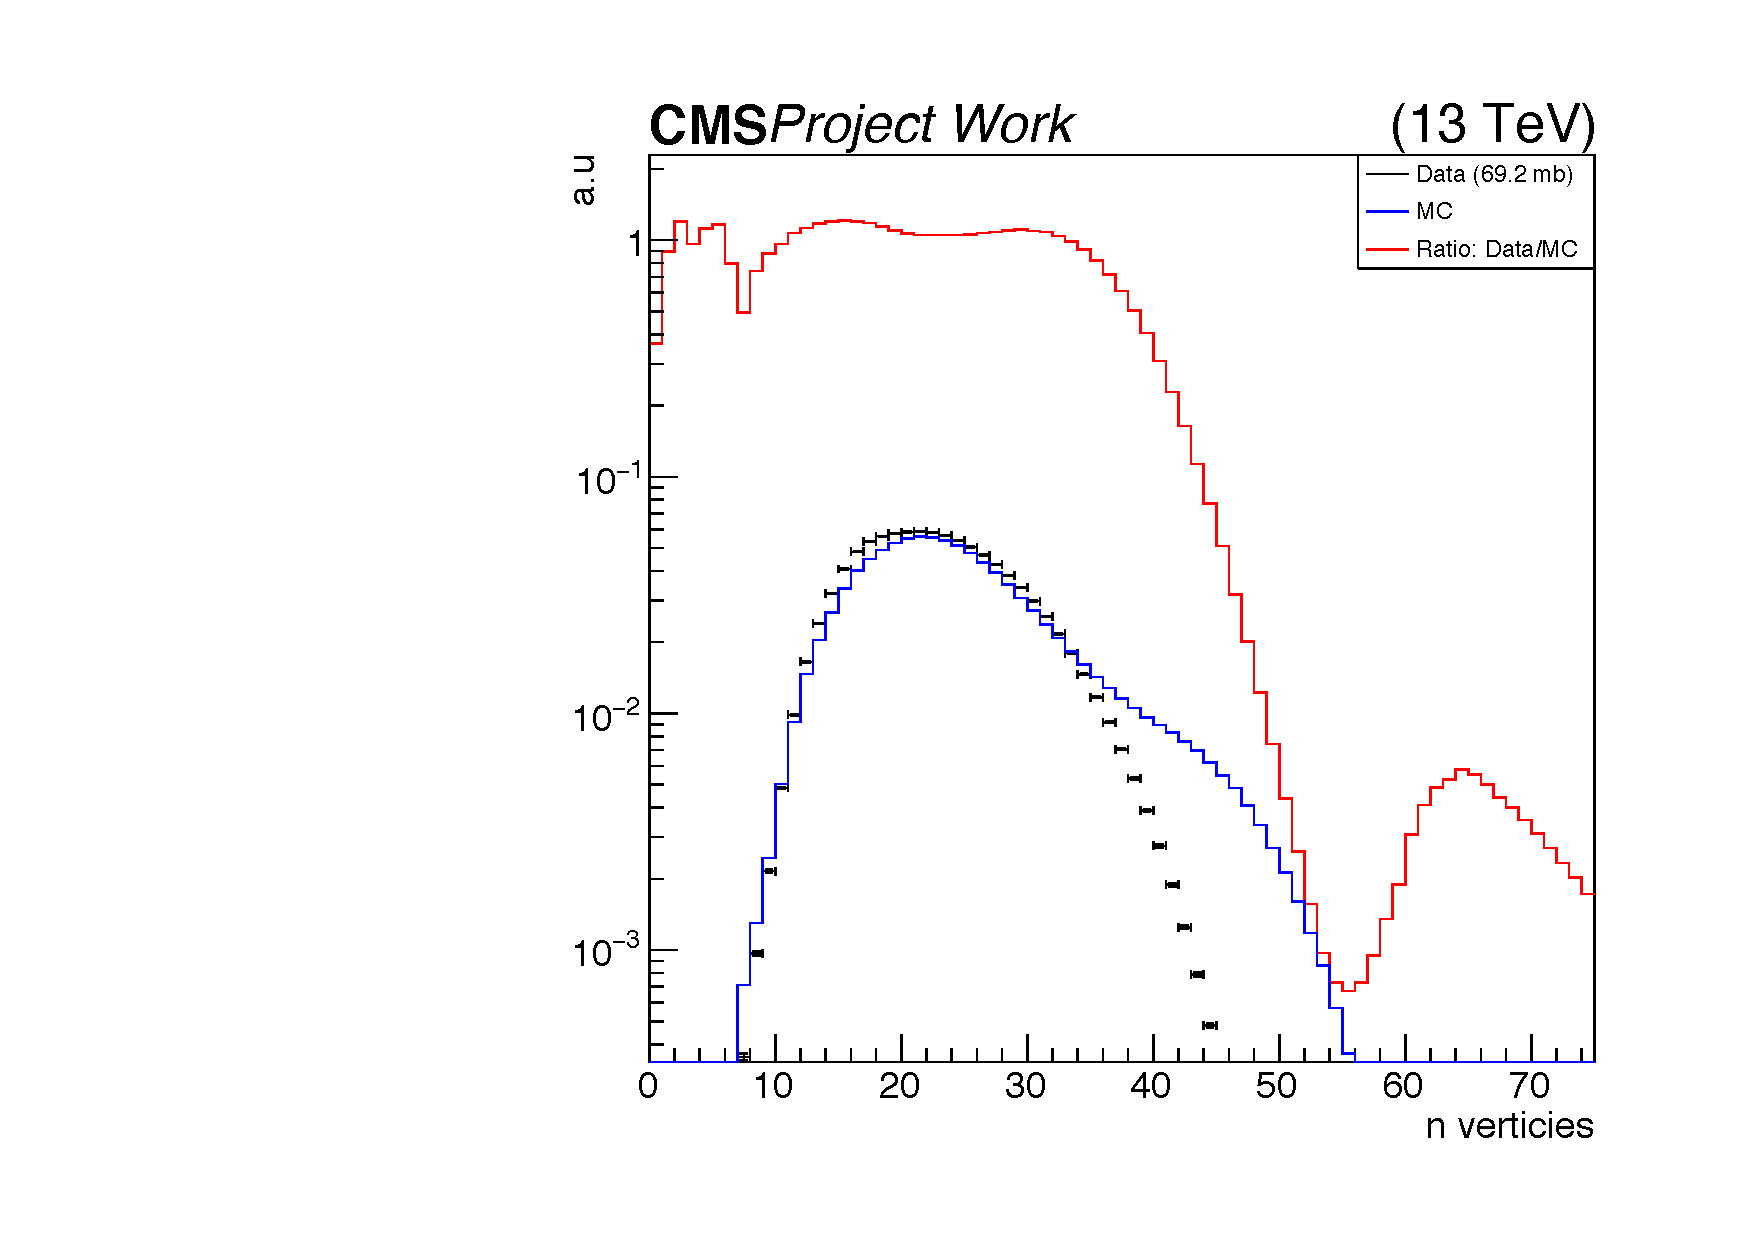
\includegraphics[width=0.6\textwidth]{Plots/analysis/pileUp/pileUp.pdf}
\centering
  \caption{\label{fig:pileUpmine} The normalised distributions of mean number of interactions per bunch crossing during the analysed data Run2016 (black) and in the MC samples (blue). And the red distribution represents the Data to MC ratio. For the data distribution the latest luminosity calibrations ~\cite{PileUp} and an inelastic pp cross-section of 69.2 mb are used. 
  }
\end{figure*}\\
\section{Baseline selection}
\label{sec:BL}
Earlier in this section \ref{signalDef}, the SUSY signature considered in this work is introduced. Moreover, a suitable primary event selection for removing the SM background as much as possible while keeping the signal efficiency high was discussed. In the following, details of this event selection are explained.\\
\textbf{Selection of leptons:}\\
The selected lepton, which can be an electron or a muon, is required to have a minimum $\pt$ of 25 GeV while at the same time it satisfies the good lepton criteria introduced in Sec. \ref{sec:PF}. Additionally, all the other electrons and muons with $\pt$ greater than 10 GeV are vetoed. These veto leptons satisfy the loose lepton selection with $I_{rel}<0.4$.
\\
\textbf{Selection of jets:}\\
The reconstruction of jets is already introduced in Sec. \ref{sec:PF}. In the present analysis, jets are required to have $\pt > 30$ GeV and $| \eta | < 2.4 $. In order to avoid double counting of objects, jets that are close ($\Delta R <0.4$) to either a veto or selected lepton are removed.
As discussed earlier in this chapter the T5qqqqWW is expected to have at least five jets. Moreover, the mass difference of the gluino and the intermediate chargino affects the $\pt$ of the jets. Therefore, it is required that two highest $\pt$ jets satisfy the $\pt >80$ GeV condition. Additionally, in the baseline selection of the analysis, the number of jets tagged as coming from b quarks is zero to suppress the events containing top quarks.
\\
\textbf{Energy scales thresholds:}\\
The signal model considered in this work favors events with high hadronic and leptonic scale. The hadronic scale is chosen to be at least 500 GeV while the leptonic scale threshold is 250 GeV.
\\
\textbf{Isolated track veto:}\\
The isolated track veto is designed to suppress $\ttbar$ events in which both W bosons decay leptonically and one lepton does not satisfy the selection criteria for veto leptons. In the mechanism of this veto, the $\MTt$ variable, which is introduced in section \ref{keyVars}, is used with an isolated track $\vec{t}$, a lepton $\vec{\ell}$ and the missing transverse momentum $\ptvecmiss$. In the calculation of $\MTt$, it is assumed that the missing energy source is the two neutrinos from the dileptonic $\ttbar$ decay. The minimization runs over all possible splitting of $\ptvecmiss$.
The figure \ref{fig:track_mt2} shows the $\MTt$ distribution seperate for hadronic and leptonic tracks after the baseline selection with $\HT > 500$ GeV, $\LT > 250$ GeV,  $\njet \geq 5$ and without b-tag requirement. The distribution of
\MTt\, is slightly different for the two cases and a lower \MTt\, cut of $60$ GeV and $80$ GeV is
applied for hadronic and leptonic tracks respectively. The rightmost plot in  the figure ~\ref{fig:track_mt2}
shows the \MTt\, distribution for all events i.e. including events that do not have any isolated track at
all. In this case events without any isolated track are added to the overflow bin. It can also be derived from the plot that only about 20\% of the signal events have an opposite charged isolated track at all compared to 40\% of the dileptonic $\ttbar$ events.
 \begin{figure*}[!hbt]
    \begin{center}
  \subfigure[\MTt\, with leptonic tracks]{ 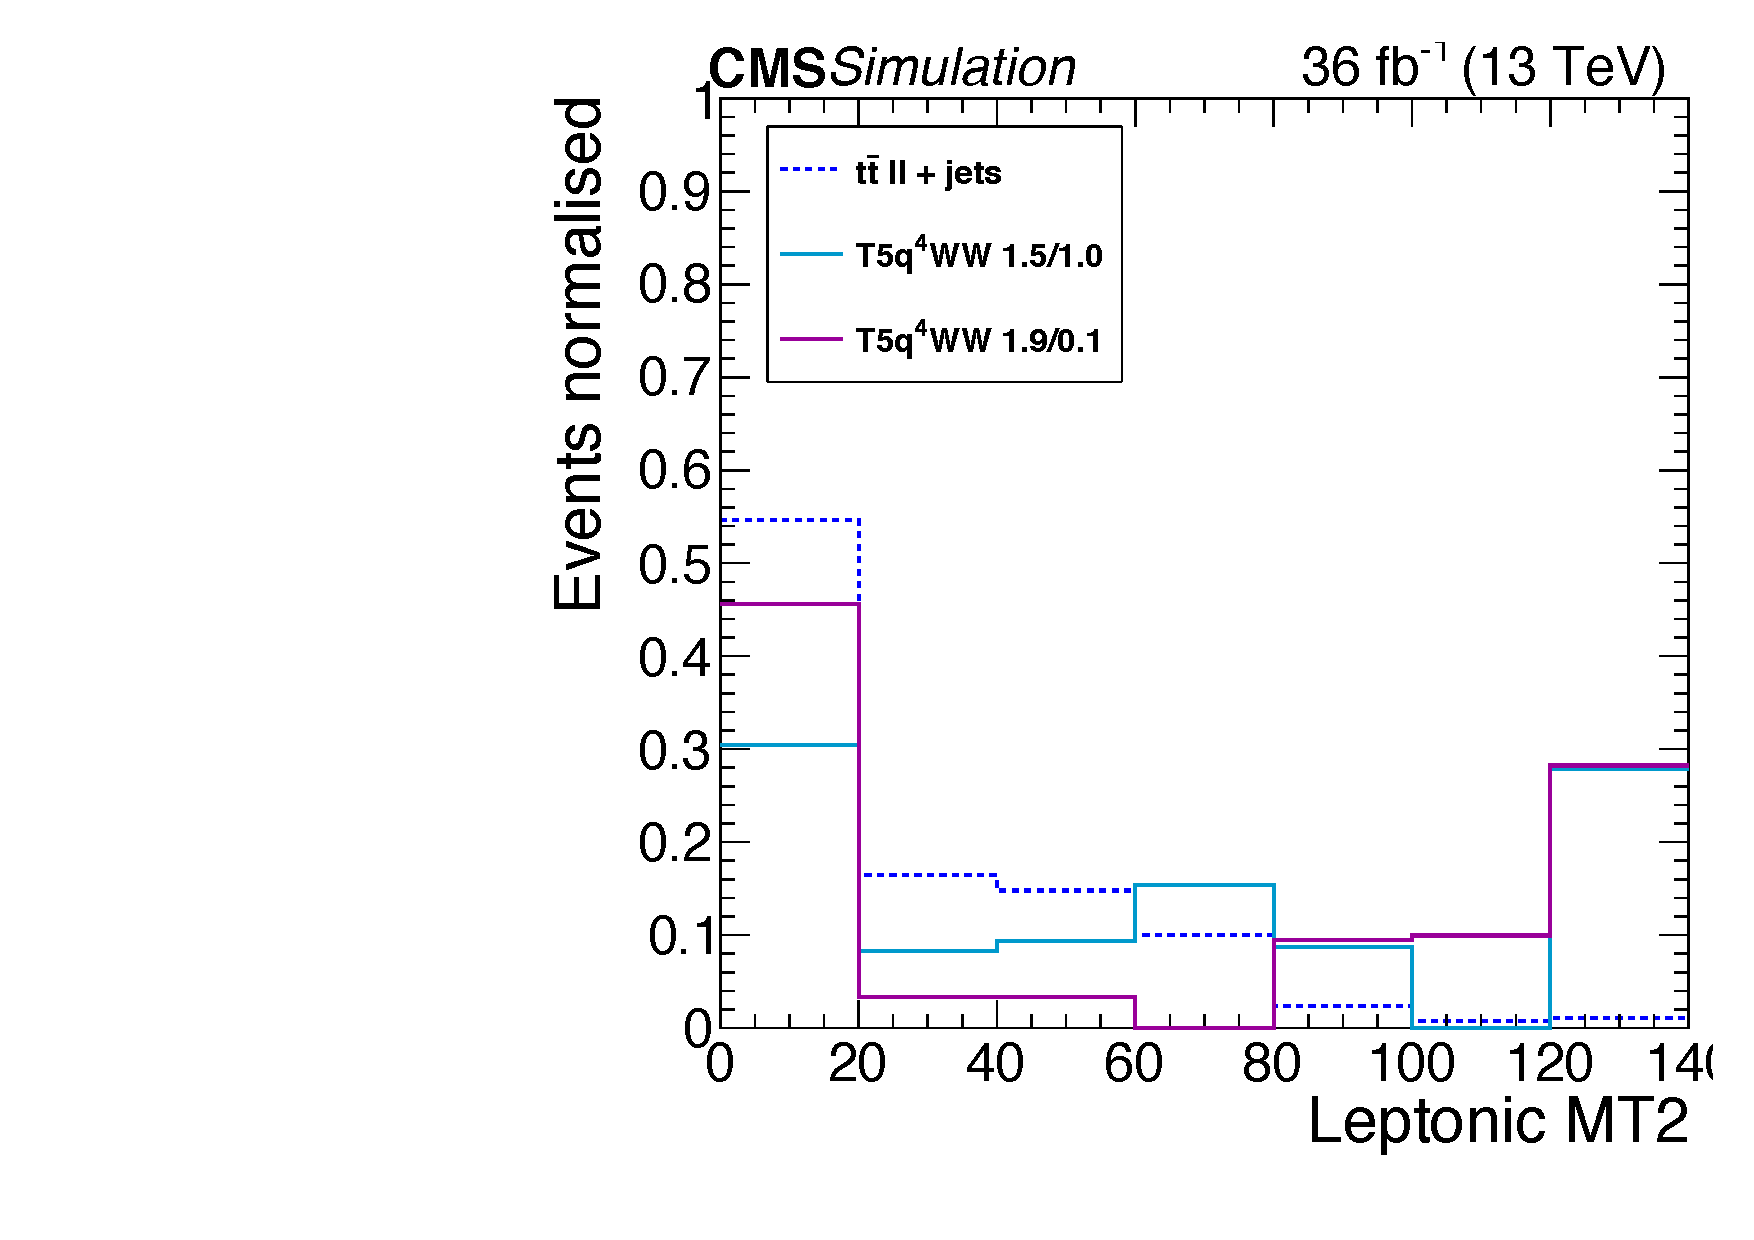
\includegraphics[width=0.3
    \textwidth]{Plots/analysis/isoveto/Mt2_nobReq_LEP.pdf}}
    \subfigure[\MTt\, with hadronic tracks]{ 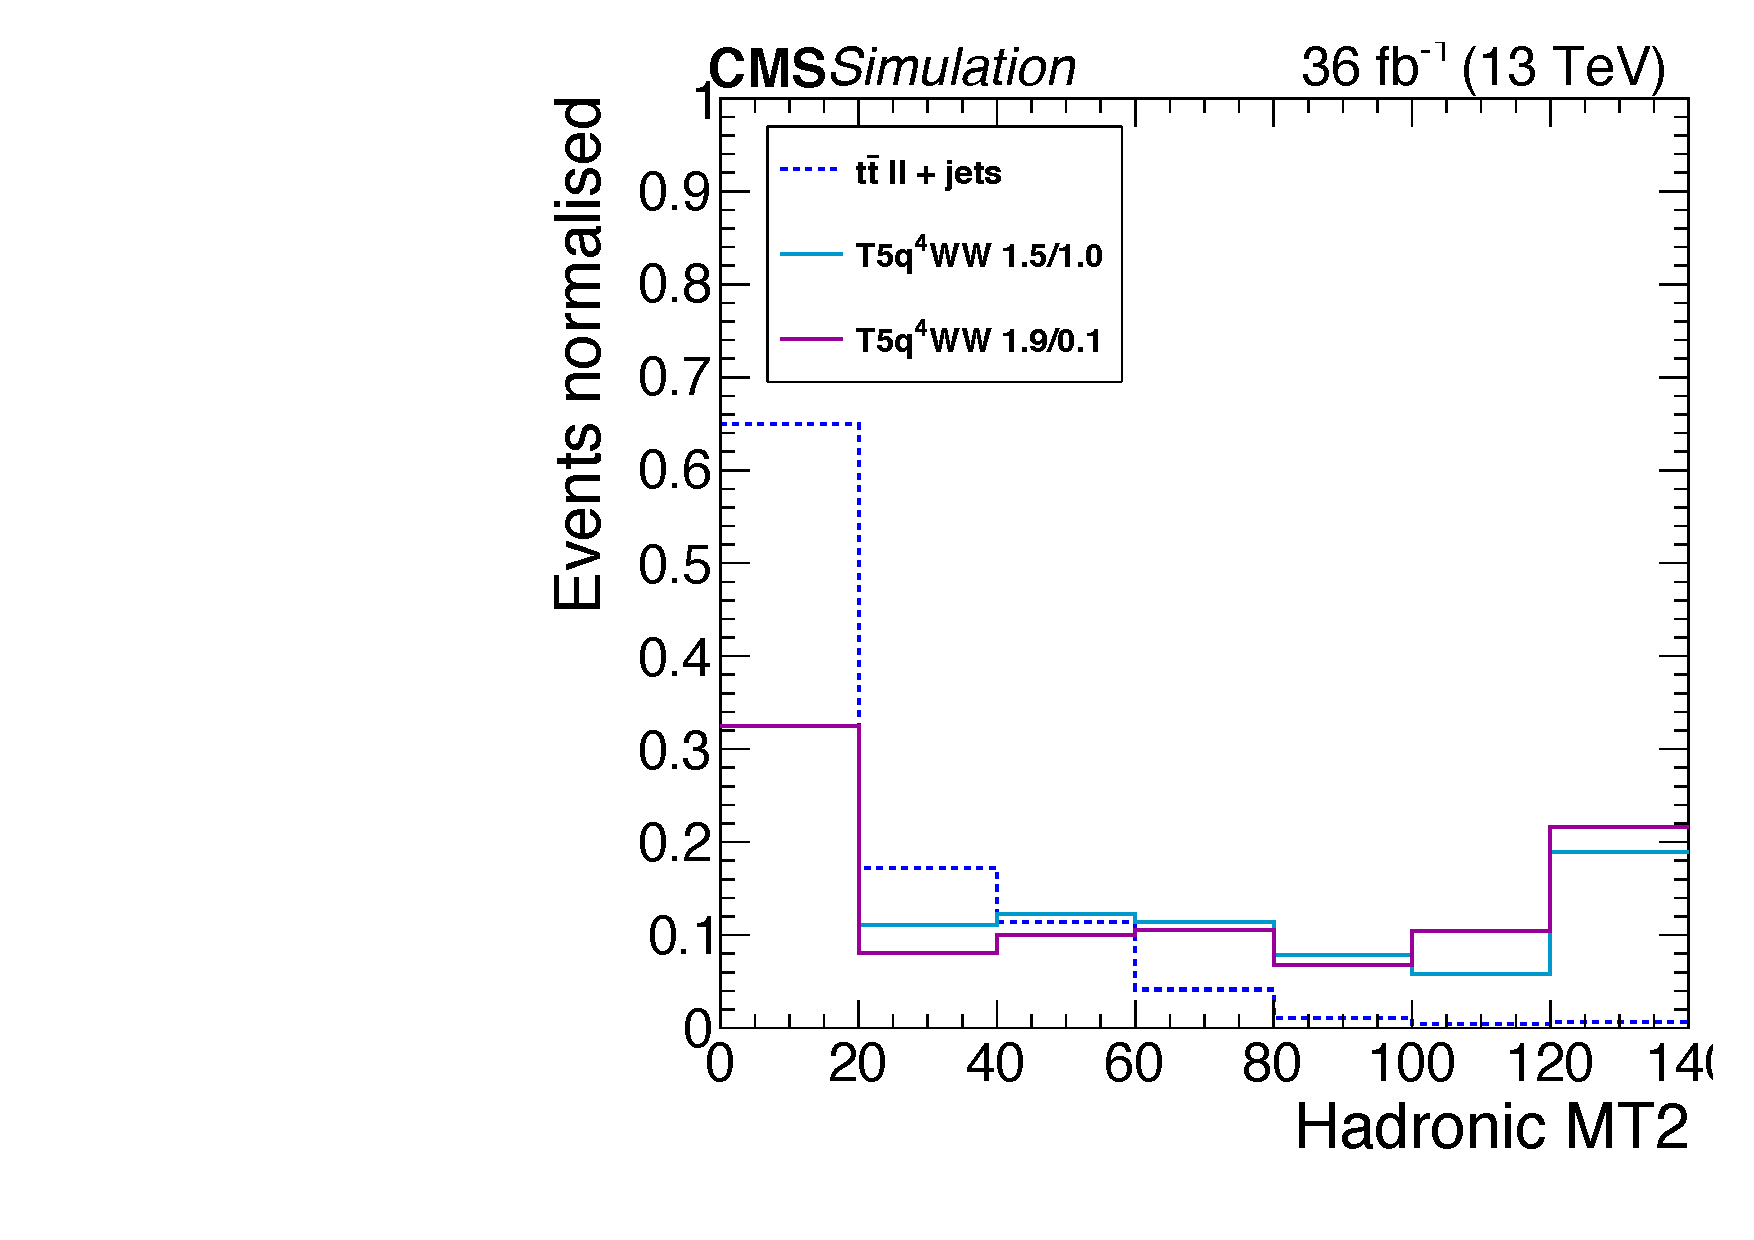
\includegraphics[width=0.3
    \textwidth]{Plots/analysis/isoveto/Mt2_nobReq_HAD.pdf}}
    \subfigure[\MTt\, (All events)        ]{ 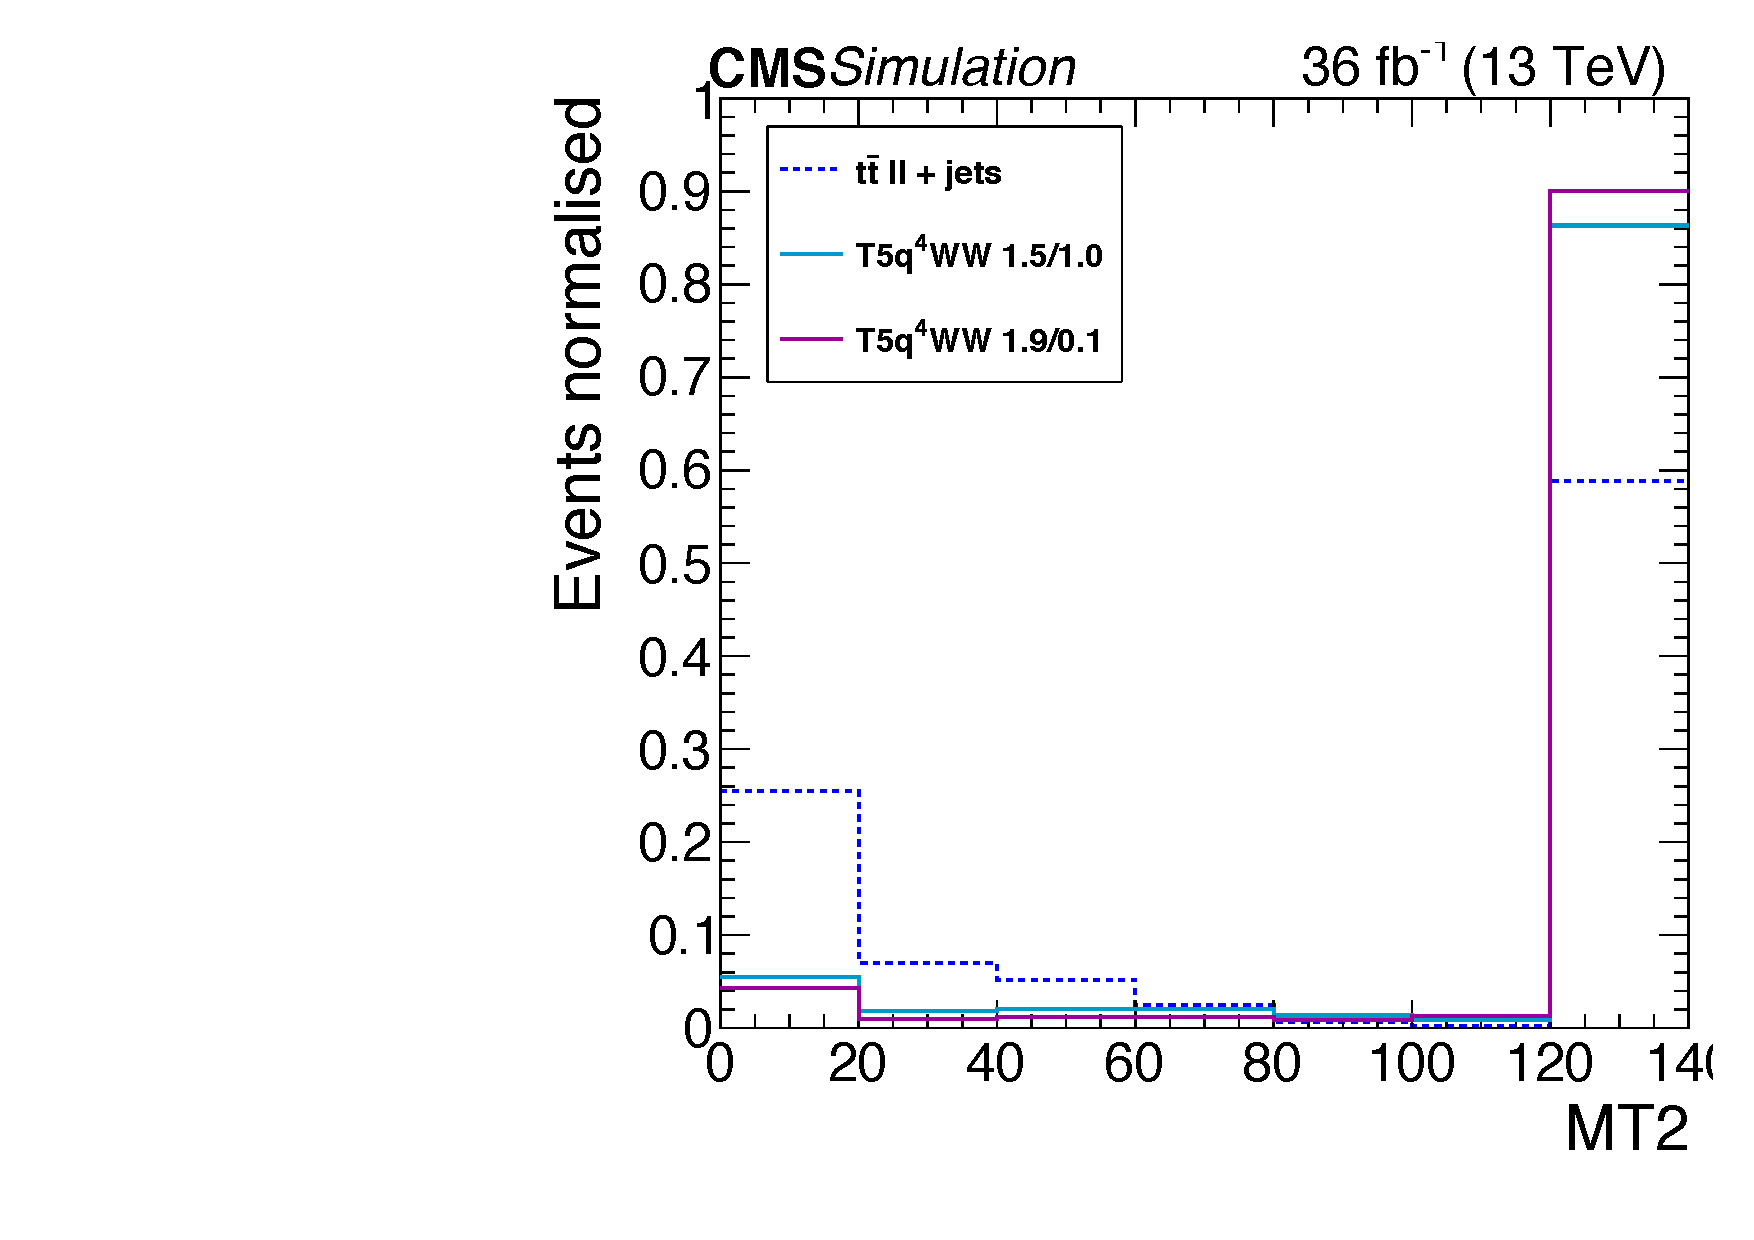
\includegraphics[width=0.3
    \textwidth]{Plots/analysis/isoveto/Mt2_nobReq_ALL.pdf}}
  \caption{ \label{fig:track_mt2} Distributions of $\MTt$ for events with electron or muon veto tracks (a) and hadronic veto tracks (b), for dileptonic $\ttbar$ (blue dotted) and T5qqqqWW (purple and azure) signal samples. The highest bin is always an overflow bin. The majority $\ttbar$ events have $\MTt < 80$ GeV, while the signal events have longer
    tails in $\MTt$.
    The rightmost plot (c) shows the distribution for all events. 
  }
   \end{center}
\end{figure*}
\\
The effect of each baseline requirement is demonstrated in Figure \ref{fig:plotFlow} for the different background processes (stacked) and for two signal benchmark points. It should be noted that the background samples include an initial skim of $\HT > 350$ GeV and $\LT > 150$ GeV to shorten the computation time. It can be observed that the design of baseline selections works such that they reduced the background events significantly while only a small fraction of signal events are eliminated by the selections. It can be also notted that, naturally, the QCD background is almost vanished after the single muon selection. The estimation of important backgrounds will be explained in the next chapter.
\renewcommand{\arraystretch}{1.5}
\begin{table}[ht]
\begin{center}
\begin{tabular}{|c|c|}\hline
Selection        & Object definitions \\
\hline
\hline
Single lepton &Tight leptons, $\pt \geq 25$ GeV and $|\eta| < 2.4$\\
                      & and $I_{mini}<0.1(0.2)$ for electrons(muons)\\\hline
Lepton veto & Loose leptons, $\pt \geq 10$ GeV and $|\eta| < 2.4$ \\
		& and $I_{mini}<0.4$ \\\hline
Isolated track veto & $I_{rel}<0.3$, $\Delta R(\ell,track) <0.1$, charge$_{track}$ = -charge$_{lepton}$  \\\hline
$n_{jets} \geq 5$ & Good jets with $\pt \geq 30$ GeV and $|\eta| < 2.4$ \\
\cline{1-1}
$p_{T,jets\,(1,2)} \geq 80$ GeV & and cleaned from close leptons \\\hline
$H_T \geq 500$ GeV & $\sum_{jets} \pt$\\\hline
$L_T \geq 250$ GeV &  $\MET + \pt^{lep}$ \\\hline
$n_{b-tag} = 0$ & b-tagged good jets with CSVv2 Medium working point (0.8484)\\\hline
\end{tabular}
\end{center}
\caption{List of event selection criteria and object requirements.}\label{tab:CutSummary}
\end{table}
\renewcommand{\arraystretch}{1}
 \begin{figure*}[!hbt]
    \begin{center}
    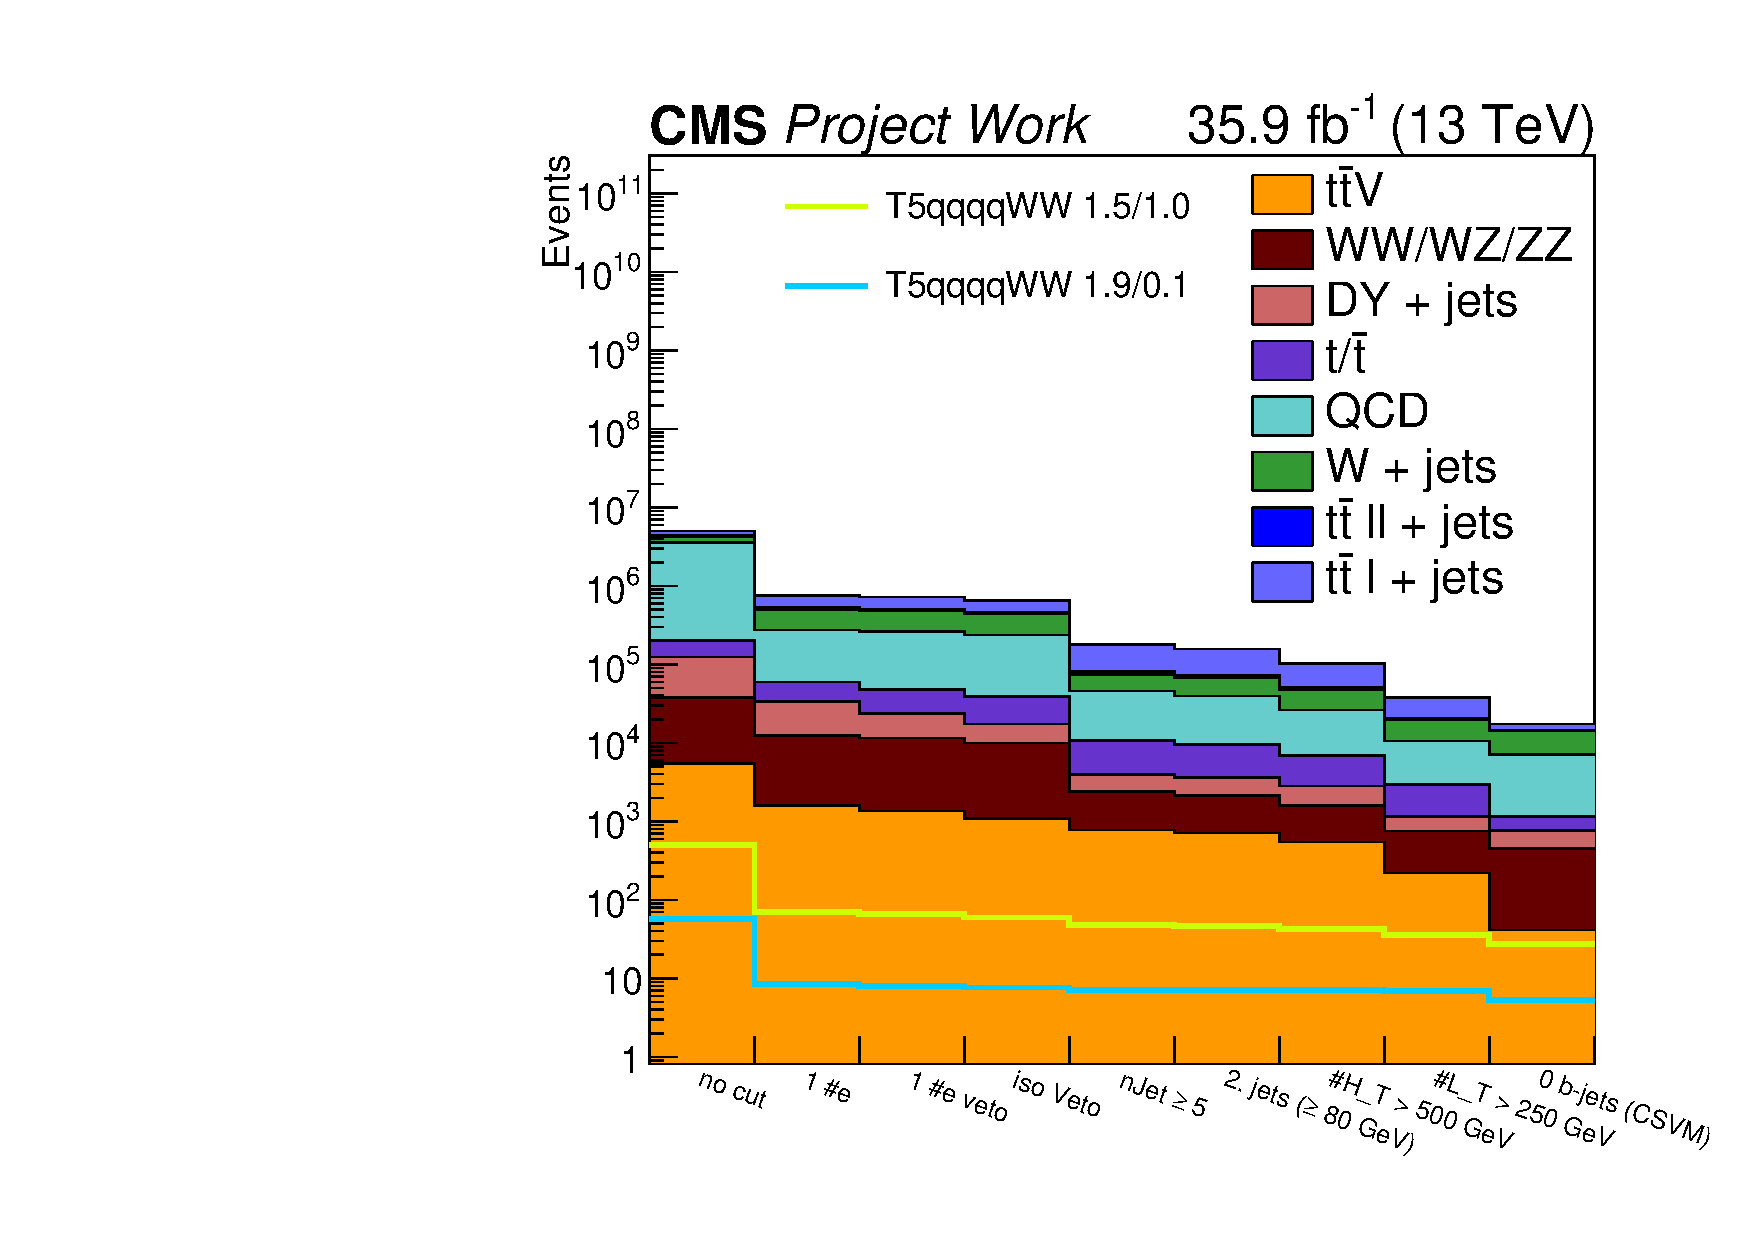
\includegraphics[width=0.45\textwidth]{Plots/analysis/cutflow/electron}
     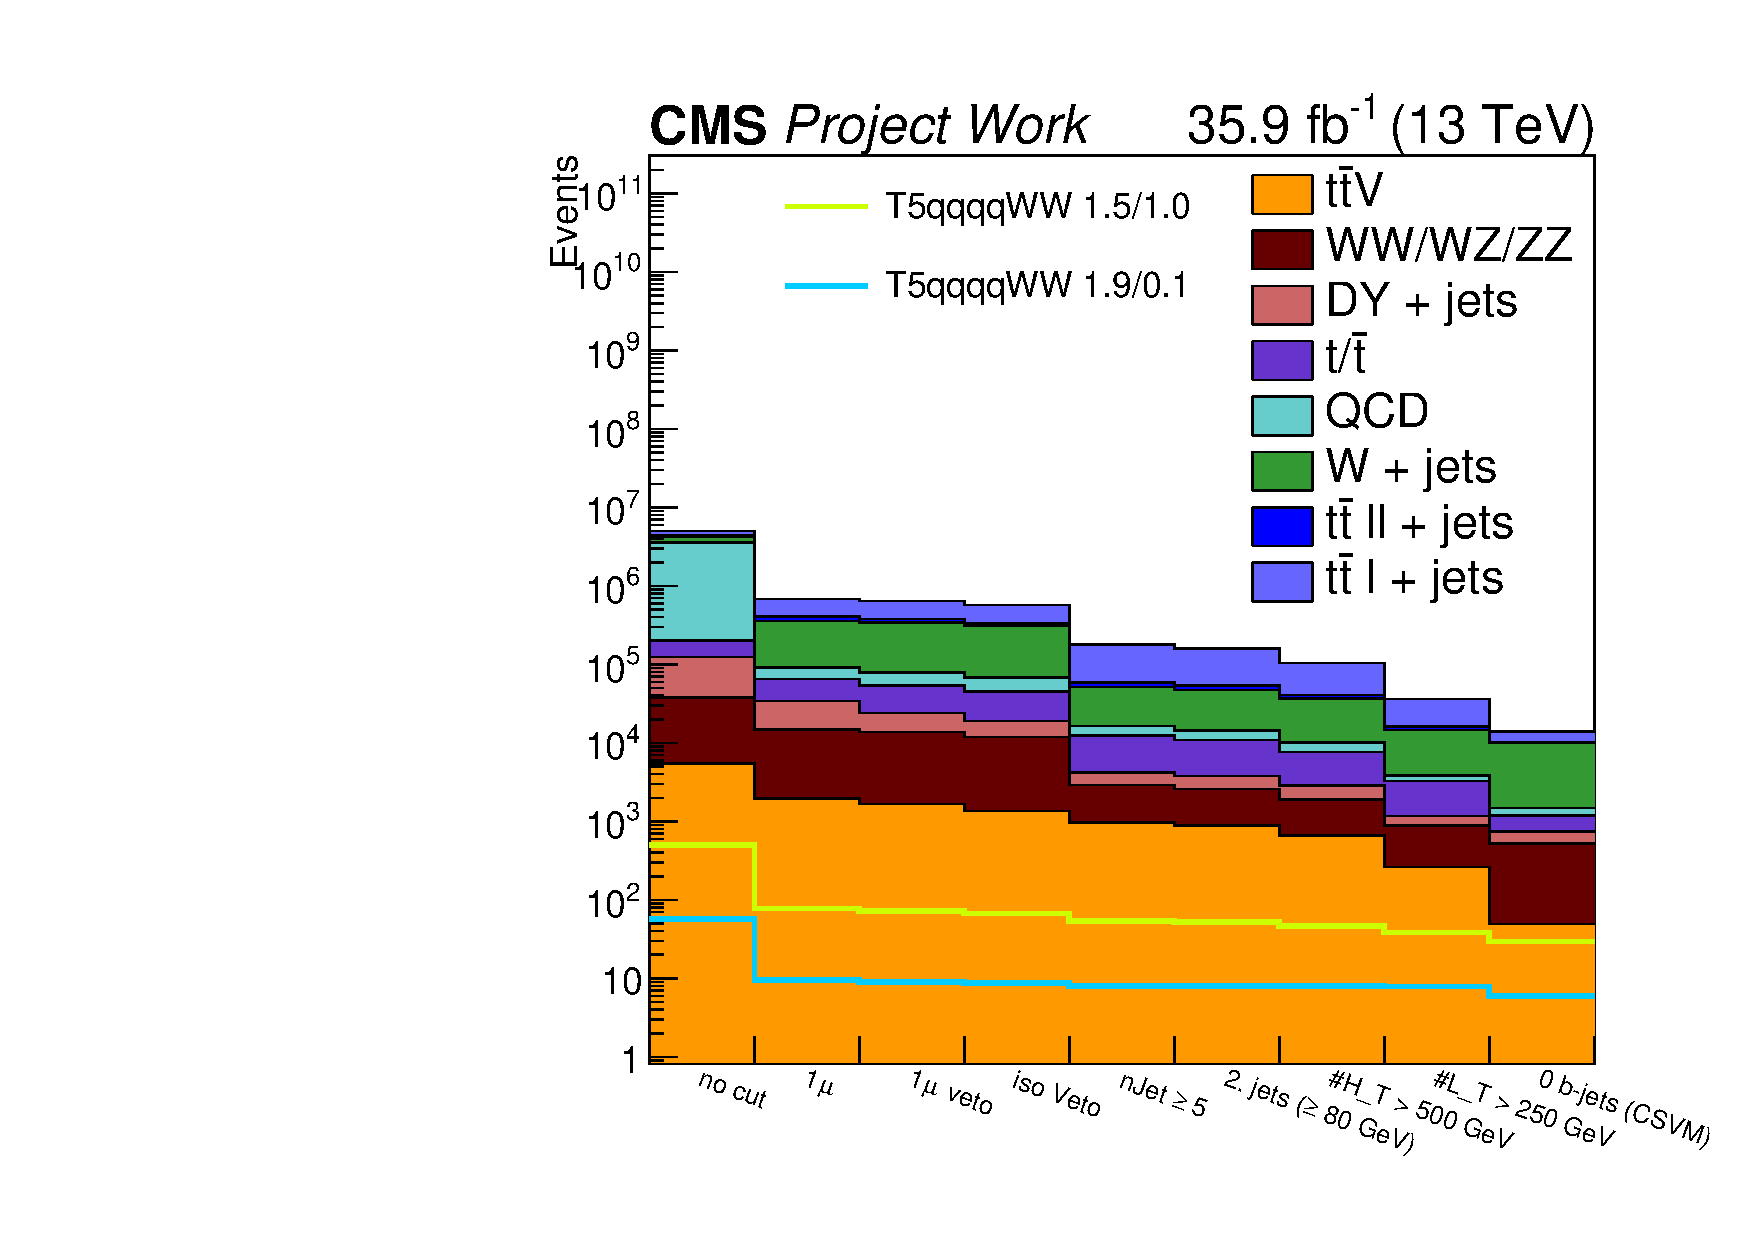
\includegraphics[width=0.45\textwidth]{Plots/analysis/cutflow/muon}
  \caption{ \label{fig:plotFlow} The number of events for each sample for the electron (left) and muon (right) channel. Samples are scaled to the luminosity with their cross section and scale factors discussed in section \ref{sec:SF}.
  }
   \end{center}
\end{figure*}
\section{Data Samples}
The data used for this analysis is recorded by the CMS detector during the 2016 LHC run at 13 TeV.  As in Figure \ref{CMSlumi},   The total integrated luminosity collected by CMS is 37.76 fb$^{-1}$. In the present analysis, the data validated by the CMS Data Quality Monitoring (CMS-DQM) certification team, which correspond to an integrated luminosity of L=35.9 fb$^{-1}$, is used. 
\subsection{Triggers}
\label{sec:triggers}
In this analysis, the main trigger set is a combination of triggers containing an isolated single lepton, electron or muon, with pT of 15 GeV and HT of 350/400 GeV.  To recover inefficiencies due to an update on the online electron ID and the saturated L1-jets, the trigger strategy had to be extended: The list of trigger paths can be seen in Table \ref{tab:triggers}.
\renewcommand{\arraystretch}{1.5}
\begin{table}[ht]
\begin{center}
\begin{tabular}{|c|}\hline
Single Electron Dataset \\
\hline
\hline
      HLT\_Ele105\_CaloIdVT\_GsfTrkIdT\_v \\
      HLT\_Ele115\_CaloIdVT\_GsfTrkIdT\_v \\
      HLT\_Ele50\_CaloIdVT\_GsfTrkIdT\_PFJet165\_v \\
      HLT\_Ele27\_WPTight\_Gsf\_v \\
      HLT\_Ele15\_IsoVVVL\_PFHT350\_v \\
      HLT\_Ele15\_IsoVVVL\_PFHT400\_v \\
\hline
Single Muon dataset \\
\hline
\hline
      HLT\_Mu50\_v \\
      HLT\_IsoMu24\_v \\
      HLT\_IsoTkMu24\_v \\
      HLT\_Mu15\_IsoVVVL\_PFHT350\_v \\
      HLT\_Mu15\_IsoVVVL\_PFHT400\_v \\
\hline
MET dataset \\
\hline
\hline
      HLT\_PFMET100\_PFMHT100\_IDTight\_ OR  HLT\_PFMETNoMu100\_PFMHTNoMu100\_IDTight\_ \\
      HLT\_PFMET110\_PFMHT110\_IDTight\_ OR  HLT\_PFMETNoMu110\_PFMHTNoMu110\_IDTight\_  \\
      HLT\_PFMET120\_PFMHT120\_IDTight\_ OR HLT\_PFMETNoMu120\_PFMHTNoMu120\_IDTight\_  \\
\hline
\end{tabular}
\end{center}
\caption{List of HLT paths}\label{tab:triggers}
\end{table}
\renewcommand{\arraystretch}{1}
Events recorded with these trigger paths are allocated in three primary datasets (PDs): the \textbf{SingleElectron}, \textbf{SingleMuon} and \textbf{MET} datasets.
Therefore, when successively adding PDs, triggers contained in previous PDs are vetoed to avoid double counting of events contained in more than one of the PDs.
The trigger efficiency calculation is shown in the Equation \ref{Eqtrig}. The trigger efficiencies are measured as a function of \LT, \, \HT\, and lepton $p_T$ and can be seen in Figures \ref{fig:trig_eff_LT}, \ref{fig:trig_eff_HT}, \ref{fig:trig_eff_leptonPt} respectively.
The efficiency distribution in the baseline region (\LT$>$250 GeV; \HT$>$500 GeV; lepton $p_T$ $>$25 GeV) is flat and its value close to 100\%(98\%) for the muons (electrons).
\begin{equation}
\label{Eqtrig}
  \epsilon = \frac{N({\rm all \; events \; passing \; probed \; trigger(s) +
  preselection + reference \; trigger})}{N({\rm all \; events \; passing
  \;preselection + reference \; trigger})}
\end{equation}

\begin{figure*}[!hbt]
  \begin{center}
    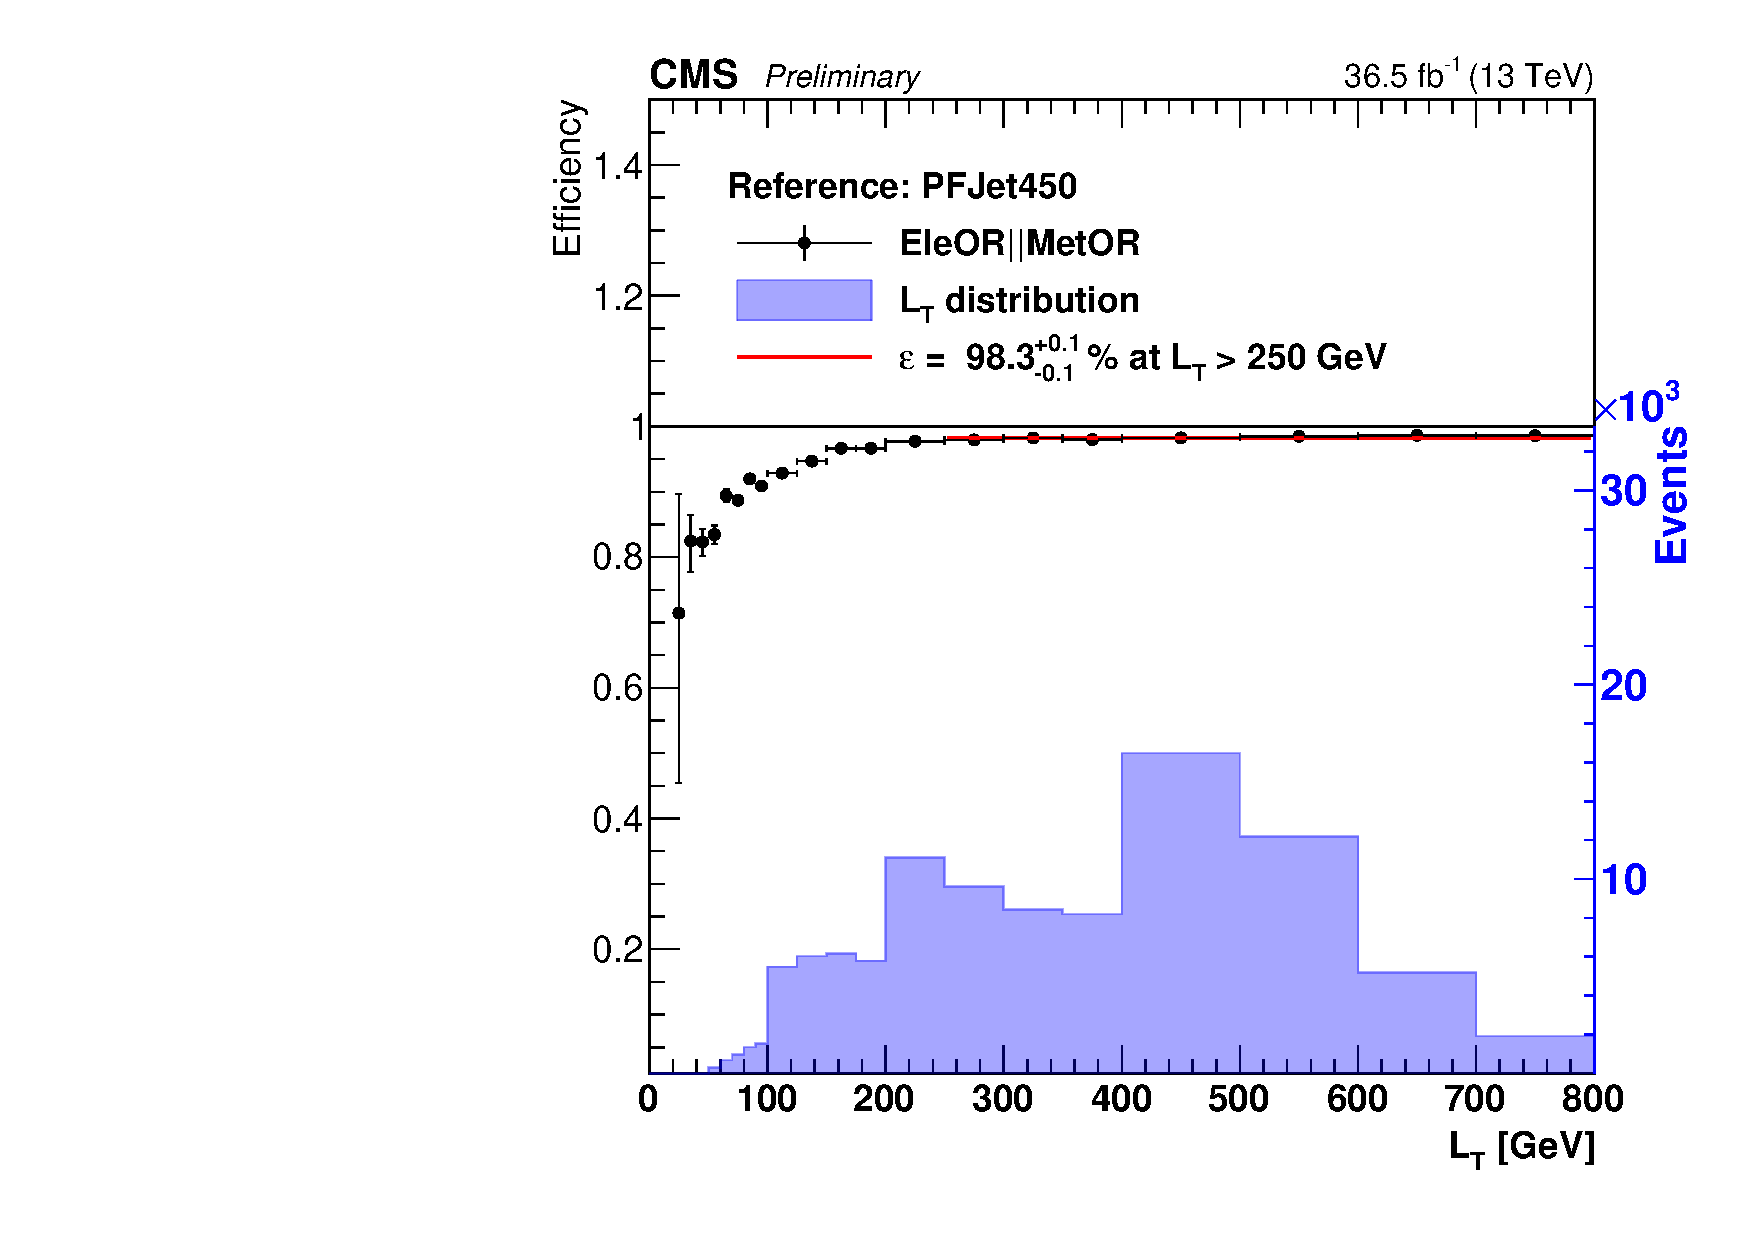
\includegraphics[width=0.4\textwidth]{Plots/trigger/LT_PFJet450_EffFit_test_HLT_EleORORHLT_MetOR.pdf}
    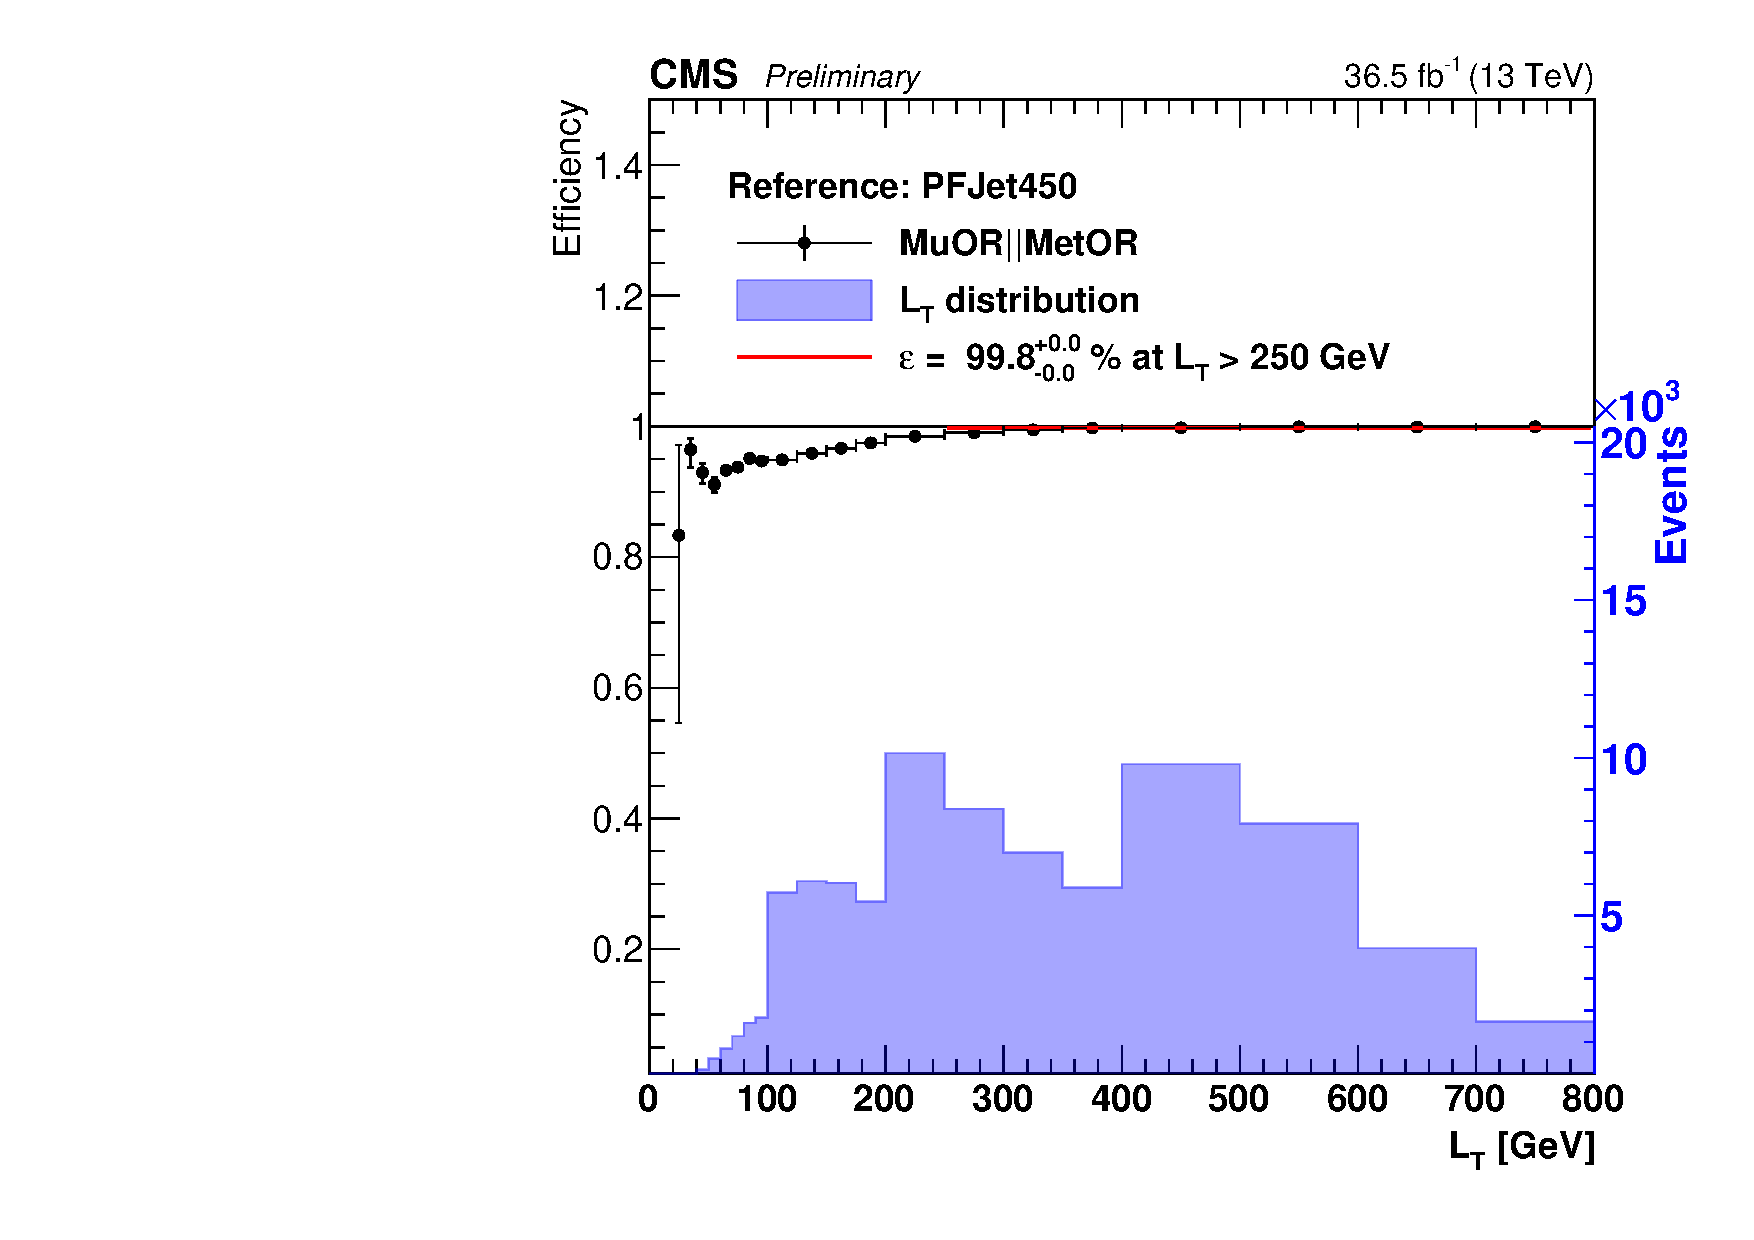
\includegraphics[width=0.4\textwidth]{Plots/trigger/LT_PFJet450_EffFit_test_HLT_MuORORHLT_MetOR.pdf}
  \end{center}
  \caption{Measurement of the trigger efficiency as a function of \LT for the
    electron trigger selection (Ele50PFJet165 / IsoEle27 / Ele105 / Ele115 /
    Ele15HT400 / Ele15HT350 / METMHTTriggers) on the left and the muon trigger
    selection (Mu50 / IsoMu24 / Mu15HT400 / Mu15HT350 / METMHTTriggers) on the
    right \cite{trigger}.
    %The number of events passing the trigger selection is given as shaded
    %histogram
  \label{fig:trig_eff_LT}}
  \end{figure*}
\begin{figure*}[!hbt]
  \begin{center}
    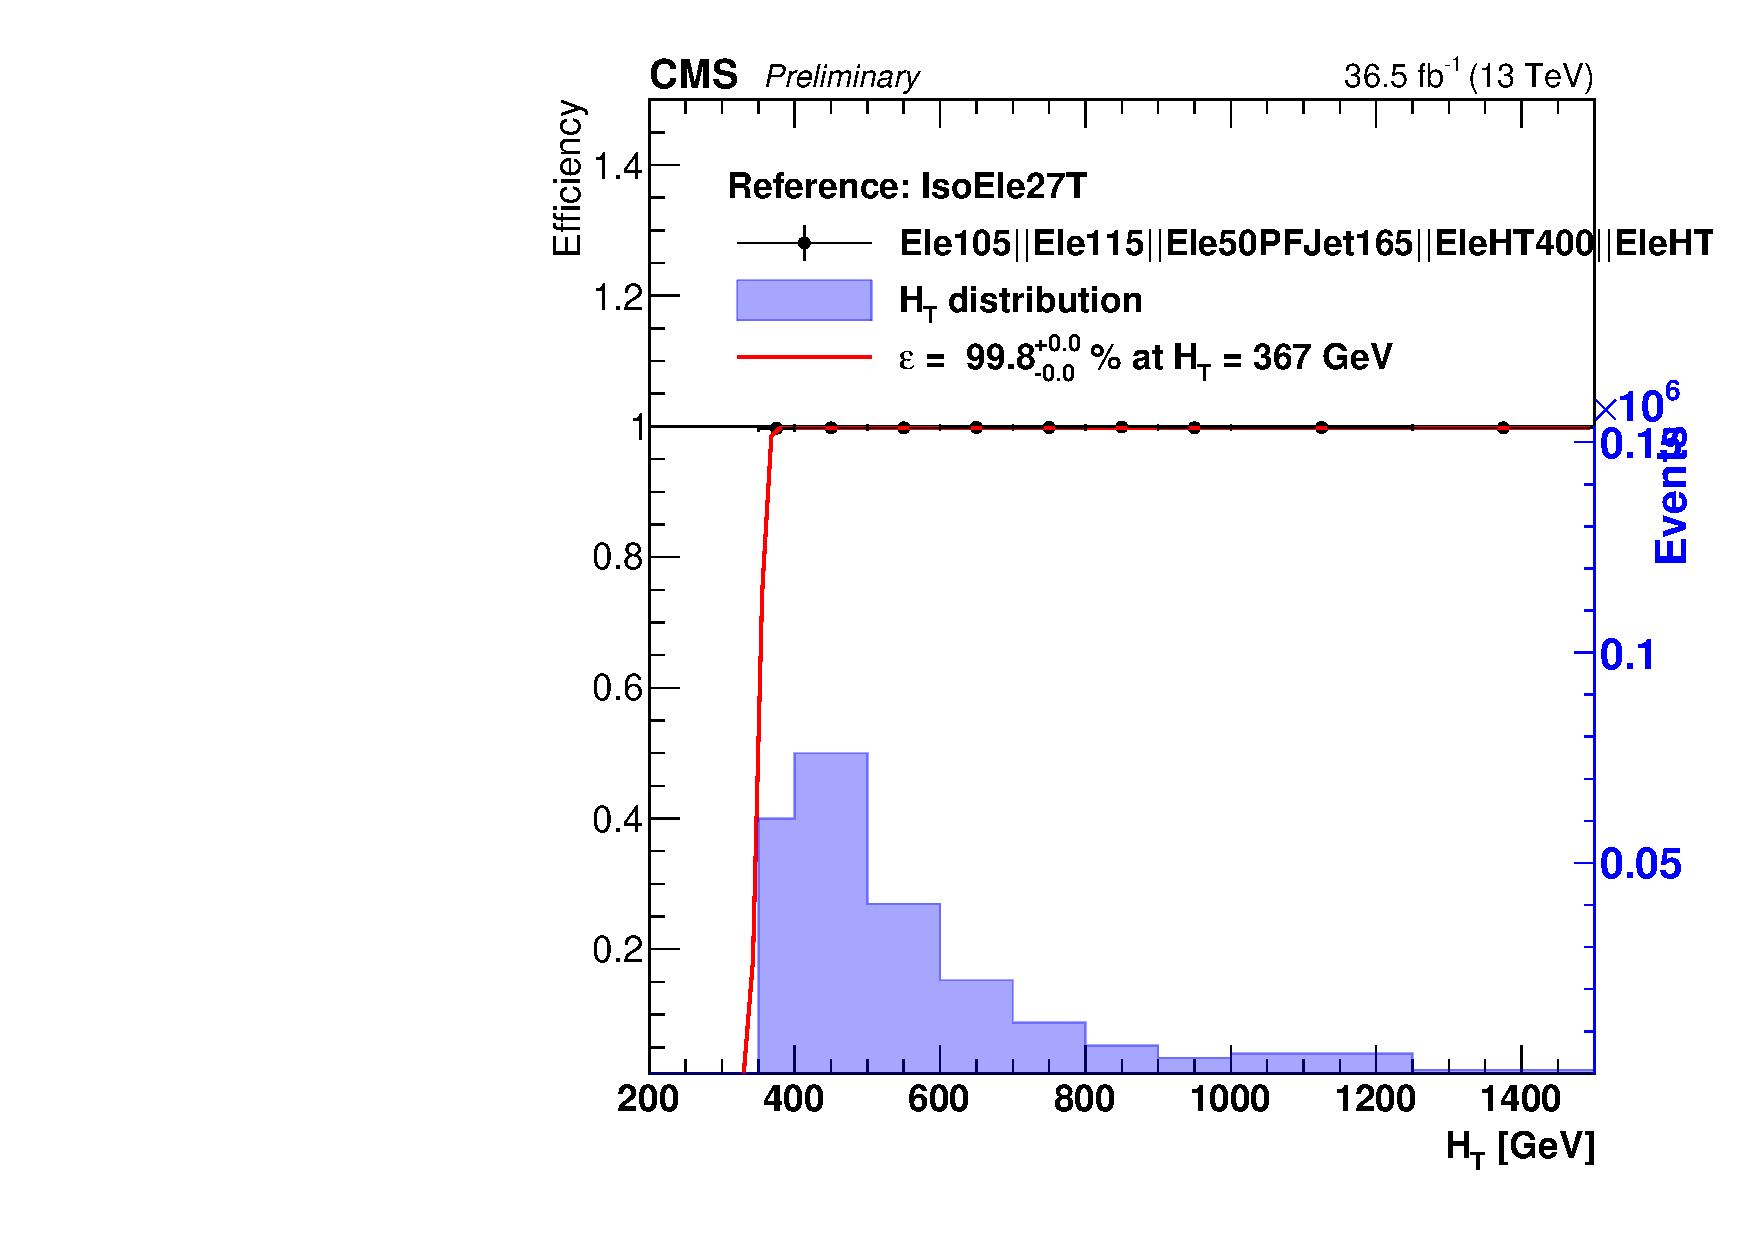
\includegraphics[width=0.4\textwidth]{Plots/trigger/HT_IsoEle27T_EffFit_test_HLT_Ele105ORHLT_Ele115ORHLT_Ele50PFJet165ORHLT_EleHT400ORHLT_EleHT350ORHLT_MetOR.pdf}
    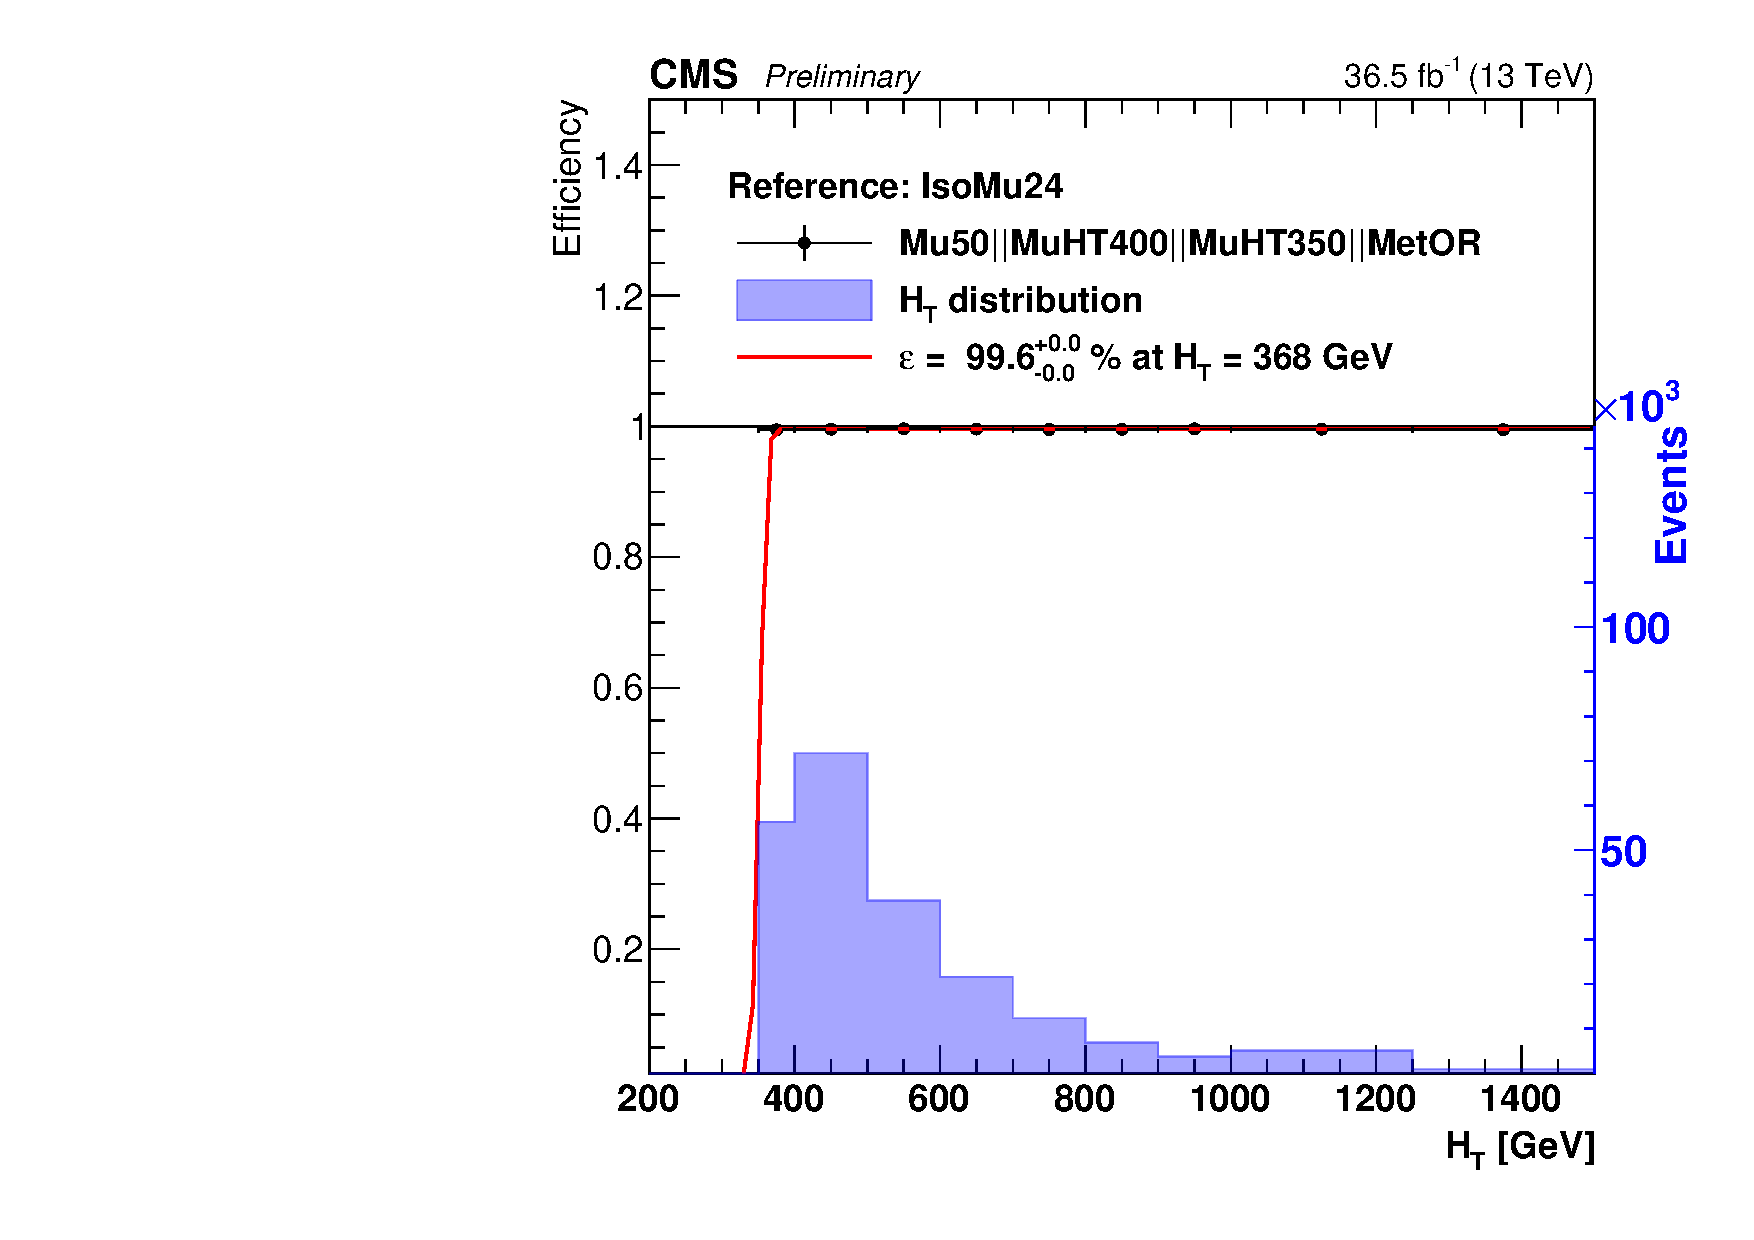
\includegraphics[width=0.4\textwidth]{Plots/trigger/HT_IsoMu24_EffFit_test_HLT_Mu50ORHLT_MuHT400ORHLT_MuHT350ORHLT_MetOR.pdf}
  \end{center}
  \caption{Measurement of the trigger efficiency as a function of \HT for the
    electron trigger selection (Ele50PFJet165 / IsoEle27 / Ele105 / Ele115 /
    Ele15HT400 / Ele15HT350 / METMHTTriggers) on the left and the muon trigger
    selection (Mu50 / IsoMu24 / Mu15HT400 / Mu15HT350 / METMHTTriggers) on the
    right \cite{trigger}.
    %The number of events passing the trigger selection is given as shaded
    %histogram
  \label{fig:trig_eff_HT}}
  \end{figure*}
  \begin{figure*}[!hbt]
    \begin{center}
    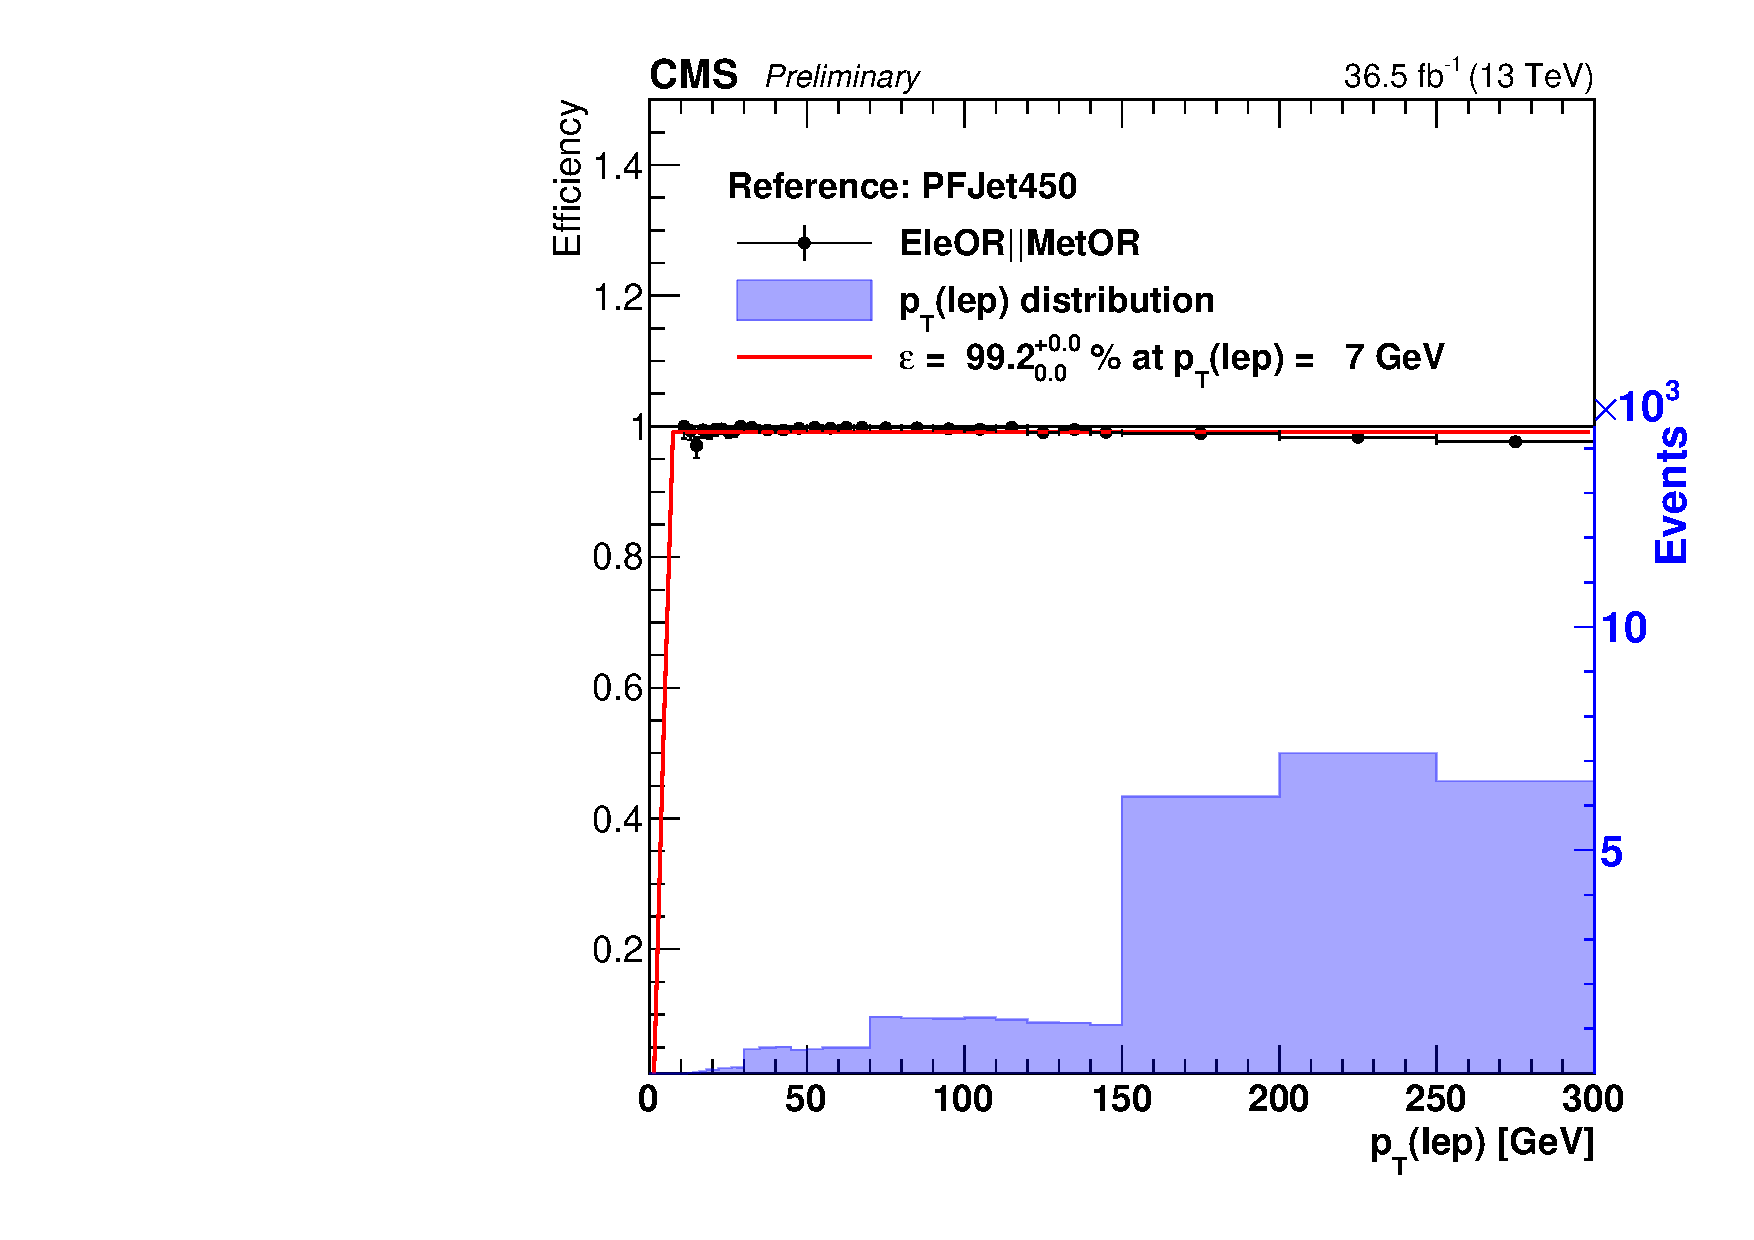
\includegraphics[width=0.4\textwidth]{Plots/trigger/LepPt_PFJet450_EffFit_test_HLT_EleORORHLT_MetOR.pdf}
    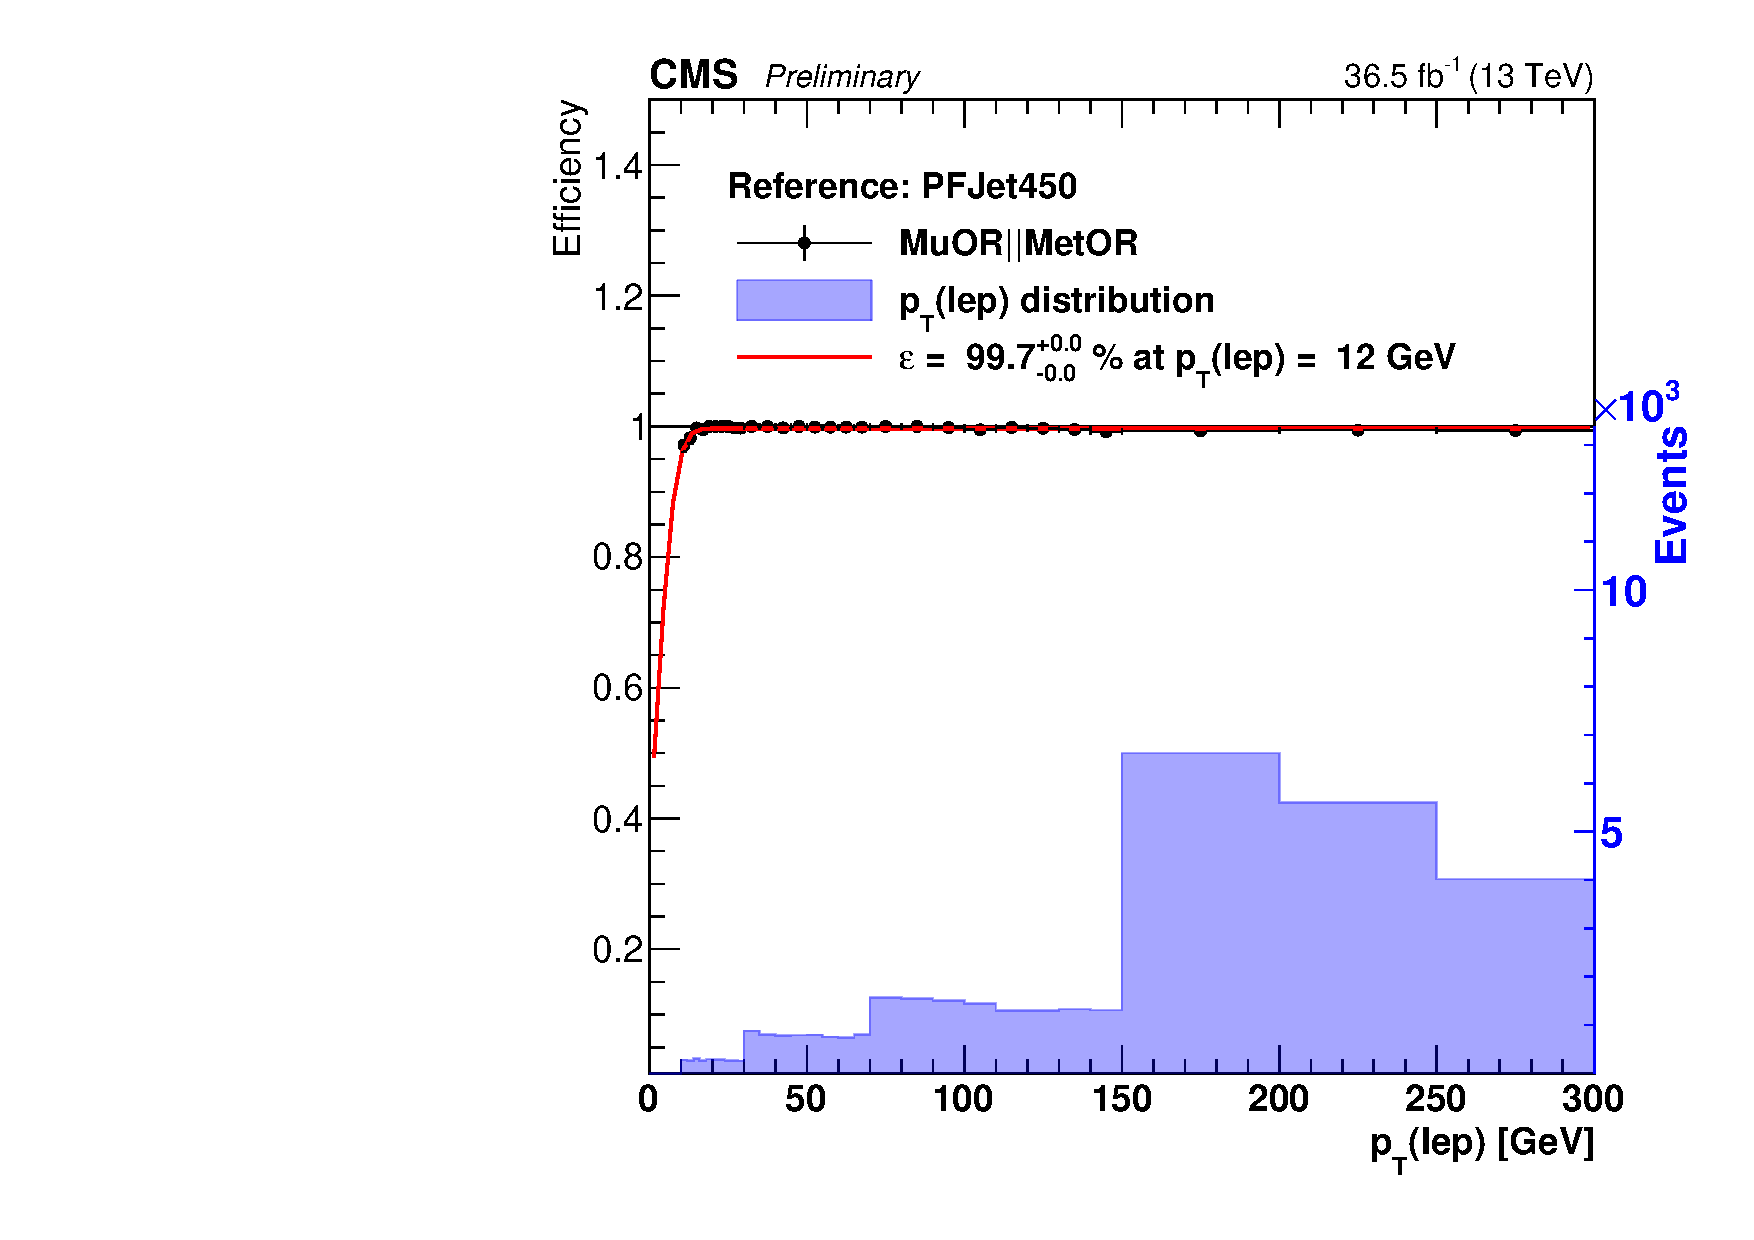
\includegraphics[width=0.4\textwidth]{Plots/trigger/LepPt_PFJet450_EffFit_test_HLT_MuORORHLT_MetOR.pdf}
  \end{center}
  \caption{Measurement of the trigger efficiency as a function of lepton $p_T$ for the
    electron trigger selection (Ele50PFJet165 / IsoEle27 / Ele105 / Ele115 /
    Ele15HT400 / Ele15HT350 / METMHTTriggers) is shown on the left and the muon trigger
    selection (Mu50 / IsoMu24 / Mu15HT400 / Mu15HT350 / METMHTTriggers) is shown on the
    right. The lepton $p_T$ trigger efficiency is measured after an $\LT>250$\,GeV cut which is the analysis baseline selection \cite{trigger}.
    %The number of events passing the trigger selection is given as shaded
    %histogram
  \label{fig:trig_eff_leptonPt}}
\end{figure*}
\section{Event cleaning: Filters}
\label{sec:filters}
The event reconstruction can fail due to the noisy detector cells and other kinds of detector problems. These can result in incorrectly reconstructed physics objects such as: muons, jets and hence MET. In CMS, the physics object groups related to the problem release event filters or cures for the falsely reconstructed objects. \\
\textbf{Primary vertex filter:}\\
A good primary vertex is required which is introduced in section \ref{sec:PV}.\\
\textbf{Beam halo filter:}\\
The collisions of the beam with residual gas inside LHC cause showers of secondary particles. Additionally to these scattering effects, charged particles are deflected by the magnetic field of the beam optics. These particles are called beam halo particles and one of the main sources of the beam background of the LHC. In CMS, the beam halo algorithm considers the particles produced outside the CMS cavern and to detect events with beam halo it uses the timing information and hit topology in CSC, ECAL and HCAL subsystems. 
\textbf{HB-HE noise filter:}\\
This noise is originated from the Hybrid PhotoDiodes and Readout Boxes of the HCAL. The timing, pulse shape as well as the other readout errors are used to detect the noise. \\
\textbf{ECAL dead cell trigger primitive filter:}\\
The existence of noisy crystals in ECAL can lead to fake MET. The events, in which the noisy cells deposit high energy, are filtered.\\
\textbf{Bad PF muon filter:}\\
This filter fires when there is a PF muon with too low quality and has large $\pt$. The quality of the muon is determined according to its tracking uncertainty, segment compatibility and other detector related features. This bad muon is required to have $\pt > 100$ GeV. Unlike the other filters explained above this filter is applied to background simulation samples as recommended. \\
\textbf{Bad charged hadron filter:}\\
The events, where there is a muon but it fails to be a PF muon and it still contributes to PF MET calculation as a charged hadron candidate, are filtered. Here, as in the previous case, this muon is required to have $\pt > 100$ GeV. Moreover, it is required that the muon and the charged hadron traces are almost overlapping ($\Delta R(\mu, charged\, hadron)<$ 0.00001). In addition to this, their $\pt$s are needed to be very close to each other. Similarly to the bad PF muon filter, this is applied to background MC samples as well as the data events. \\
\textbf{Duplicate muon filters:}\\
In the Re-reco data it is observed that there is an increase in events in the MET tail of Z$\rightarrow\mu\mu$ data. It is understood by the muon POG that there are dublicate muons in the events due to reconstruction failures. 
Additionally, two filters are recommended by the SUSY group:  
One is to remove events with the ratio of PF MET to calorimeter MET is more than 5.  The second is to remove events containing bad jets which have $\pt > 200$ GeV, muon energy fraction $>0.5$ and $\Delta\phi(met,jet)>\pi-4$.\\
\textbf{Filter on fastsim:}\\
This filter is to clean up bad jets from the fastsim events. To remember, in this work, fastsim is used for the signal MC production. The event is removed if there is a jet satisfying the following conditions:  $\pt > 20$ GeV, $|\eta|<2.5$, unmatched to a generated jet ($\Delta R(jet,gen\,jet)>0.3$), and charged hadron fraction $<$ 0.1.
\\
\\
The efficiency of all these filters after the analysis baseline selection is approximately 98\%.

\section{Control plots}
The distributions of main kinematic variables, also called control plots, are shown in this section. In all the control plots, the colored lines represent the signal models and the color filled stacked histograms display the background processes. Additionally, the black dotted distribution exhibits the observed data points requiring the triggers introduced in section \ref{sec:triggers}. In all the control plots, the events are cleaned by the filters discussed in section \ref{sec:filters}. The signal and background events are scaled by the luminosity factor and additional weights introduced in section \ref{sec:SF}. In the Figure \ref{fig:baselineplots} top left plot shows the n-btag distribution after the baseline selection (see section \ref{sec:BL}). The distribution of simulated signal events peaks at zero as expected. Clearly, one can see from this distribution that choosing events with zero b-tagged jets suppresses the $\ttbar$ background significantly. The other distributions, displaying main kinematic variables, exhibit reasonable MC-data agreement although it is not necessarily expected. The plot shows the number of jet distribution (top/right), $\HT$ (bottom/left) and $\LT$ (bottom/right) are shown. \\
The multiplicities of jets and b-tagged jets display no difference between the signal scenarios, since the mass splitting has no effect on the decay topology. 
The two selected signal benchmark models show differences in the distributions of $\HT$ and $\LT$, this is due to the gluino-neutralino mass splitting. In the non-compressed T5qqqqWW (1900,100) model, the quarks coming from the gluino decay have a large boost, resulting in high leptonic and hadronic energy scales. For the compressed region with T5qqqqWW (1500,1000) no such effect is observed, and the shape of the distributions look similar to the SM processes. \\
Additional control plots are shown in Appendix \ref{sec:CRplots}. 
 \begin{figure*}[!hbt]
    \begin{center}
 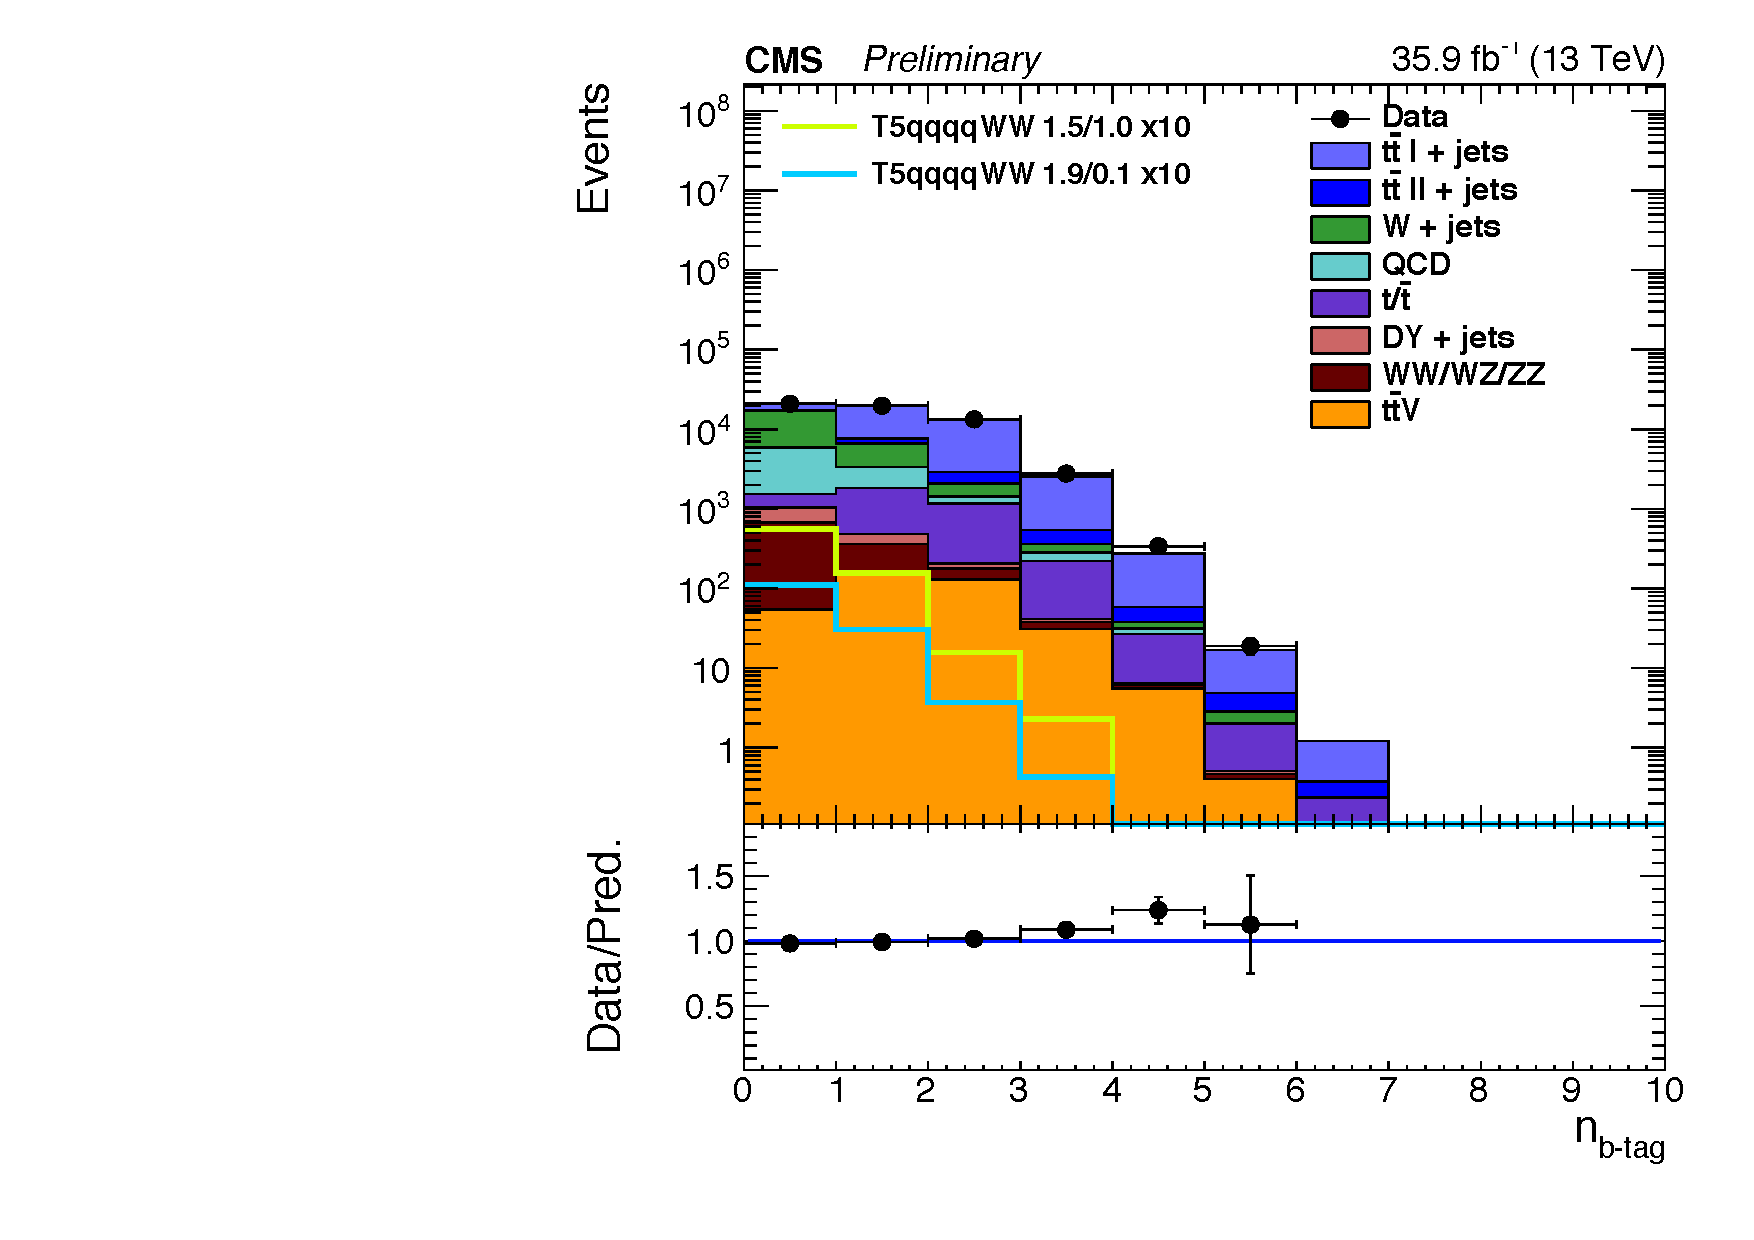
\includegraphics[width=0.45 \textwidth]{Plots/analysis/control_Plots/nBjet0b}
 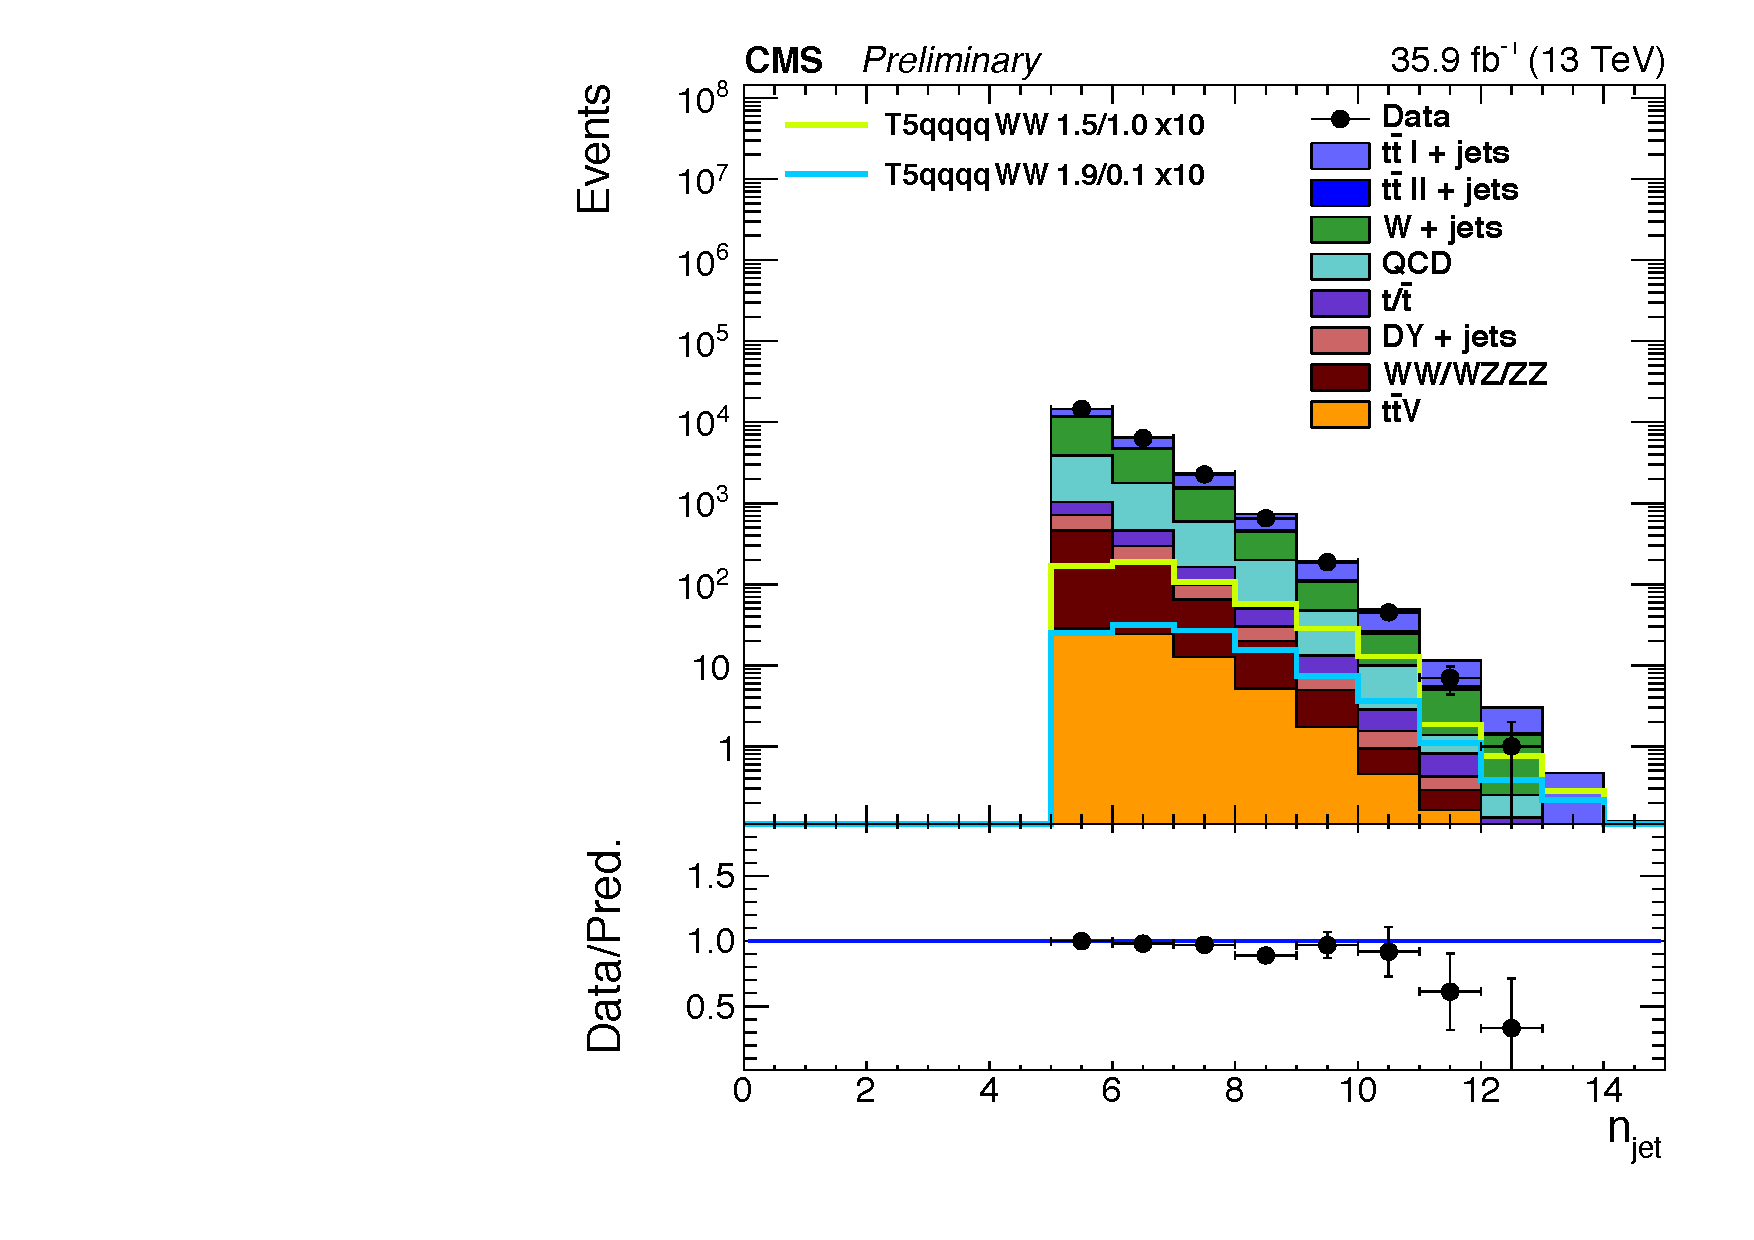
\includegraphics[width=0.45 \textwidth]{Plots/analysis/control_Plots/plots_zerob_st250_ht500_njet5_nbtagEq0_nJet30Preliminary}\\
 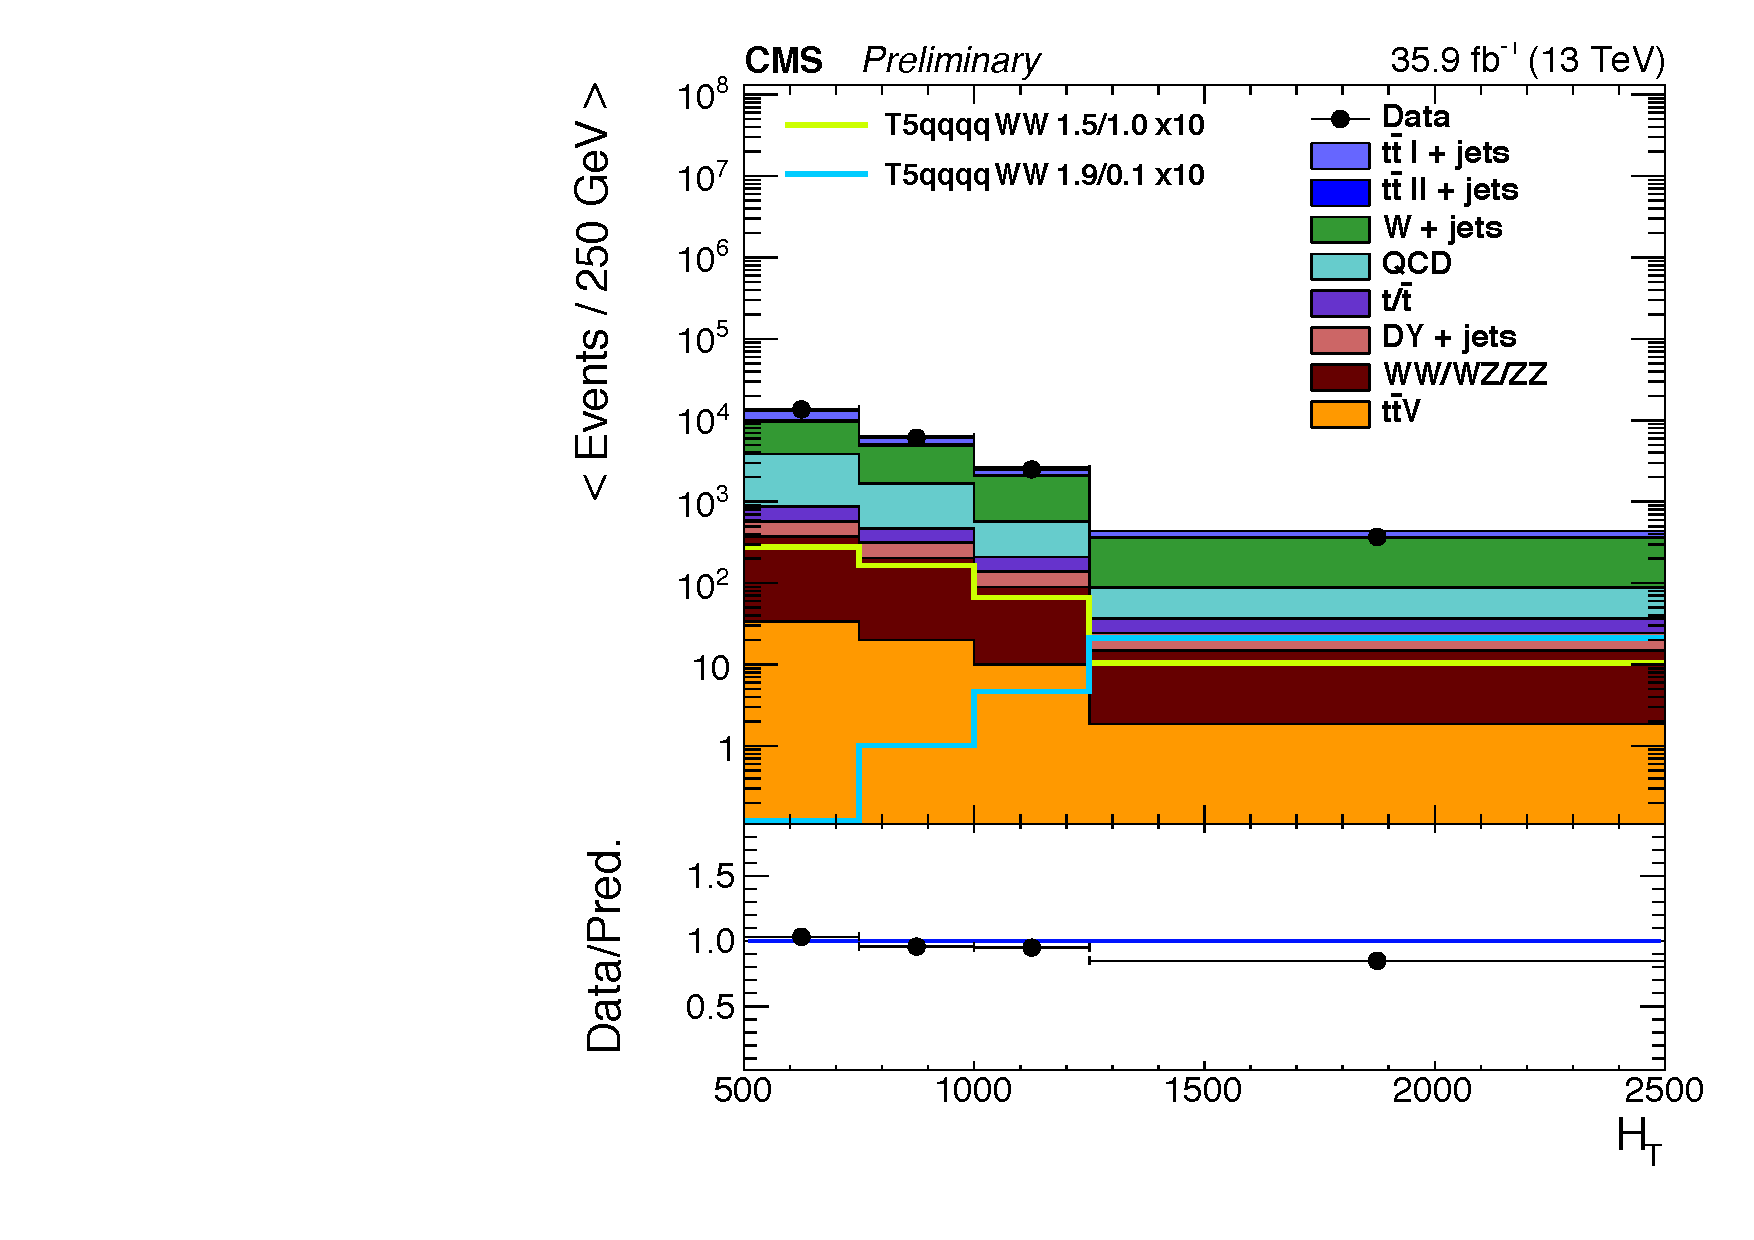
\includegraphics[width=0.45 \textwidth]{Plots/analysis/control_Plots/plots_zerob_st250_ht500_njet5_nbtagEq0_htJet30jPreliminary}
 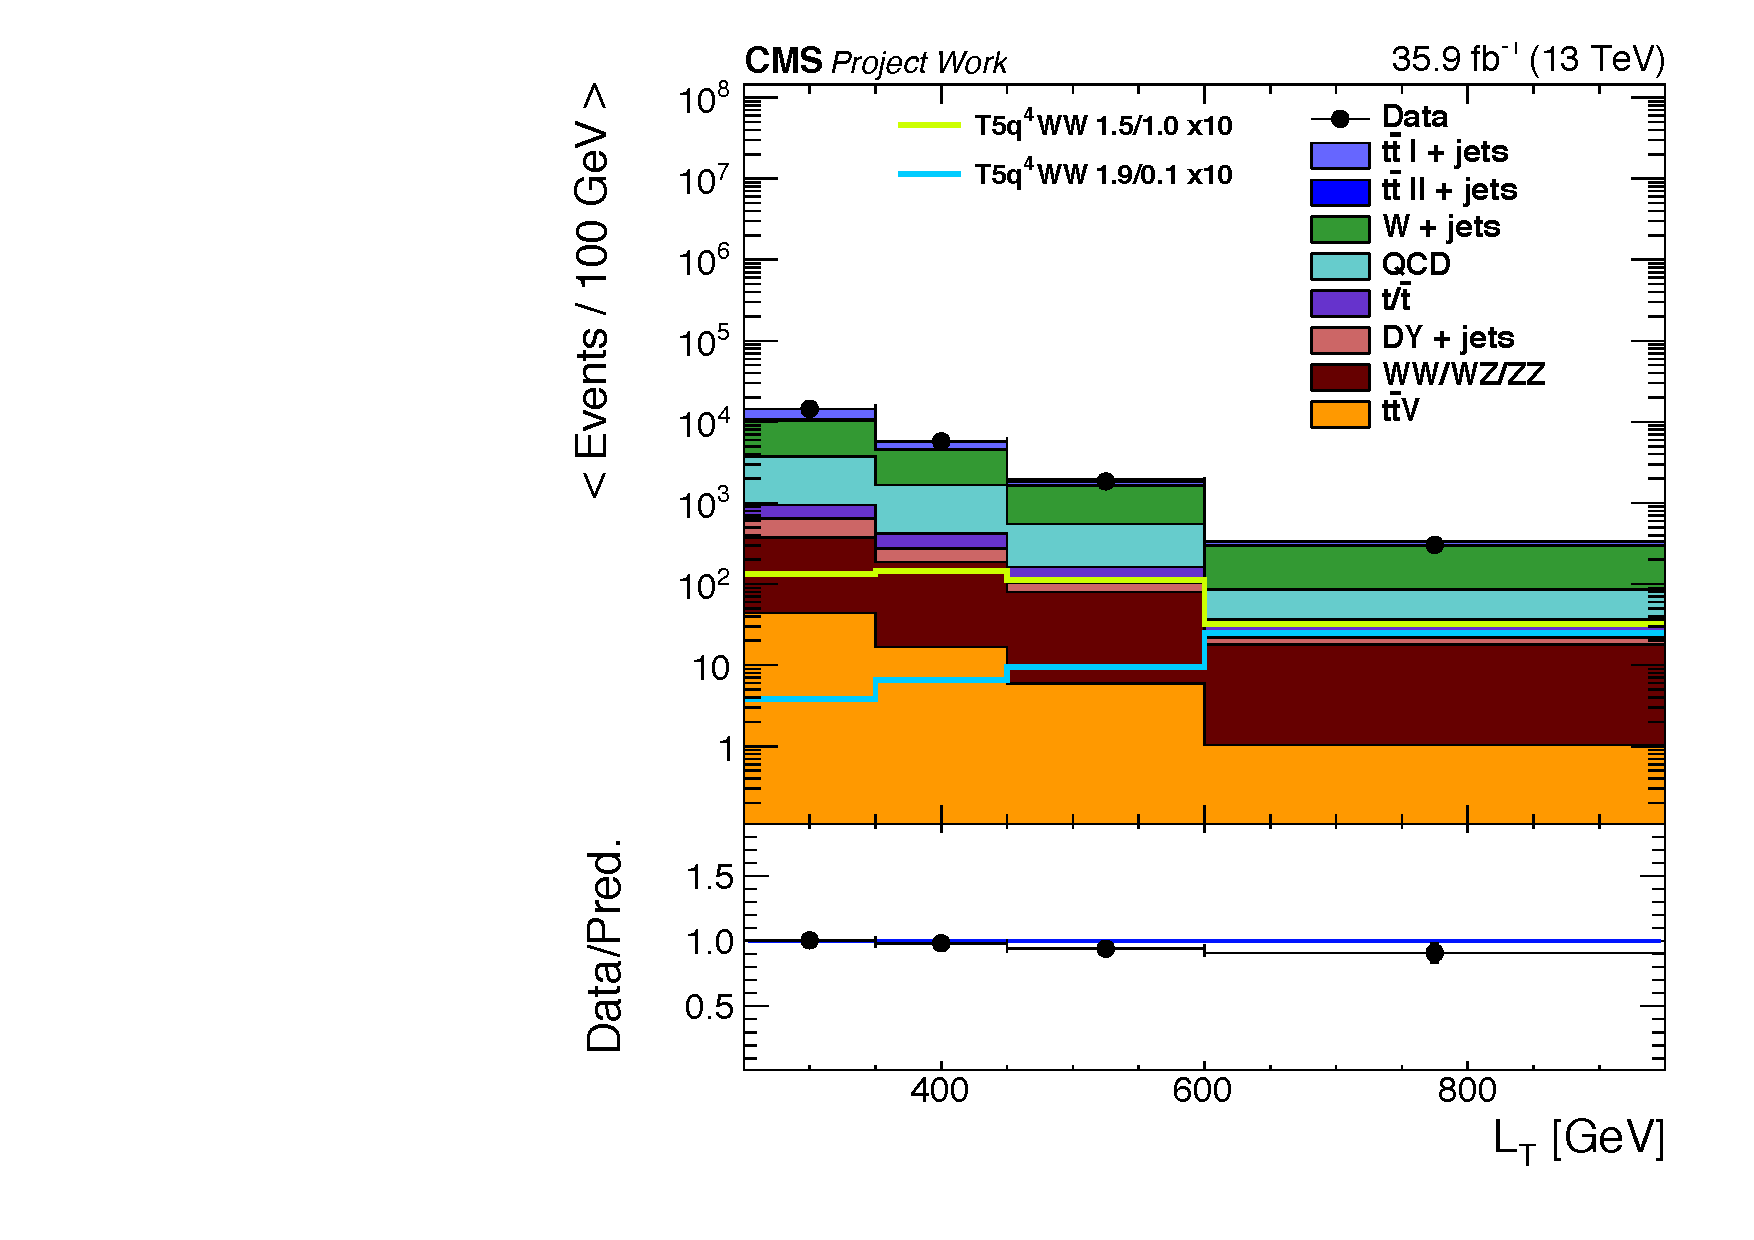
\includegraphics[width=0.45 \textwidth]{Plots/analysis/control_Plots/LT_colors}
 %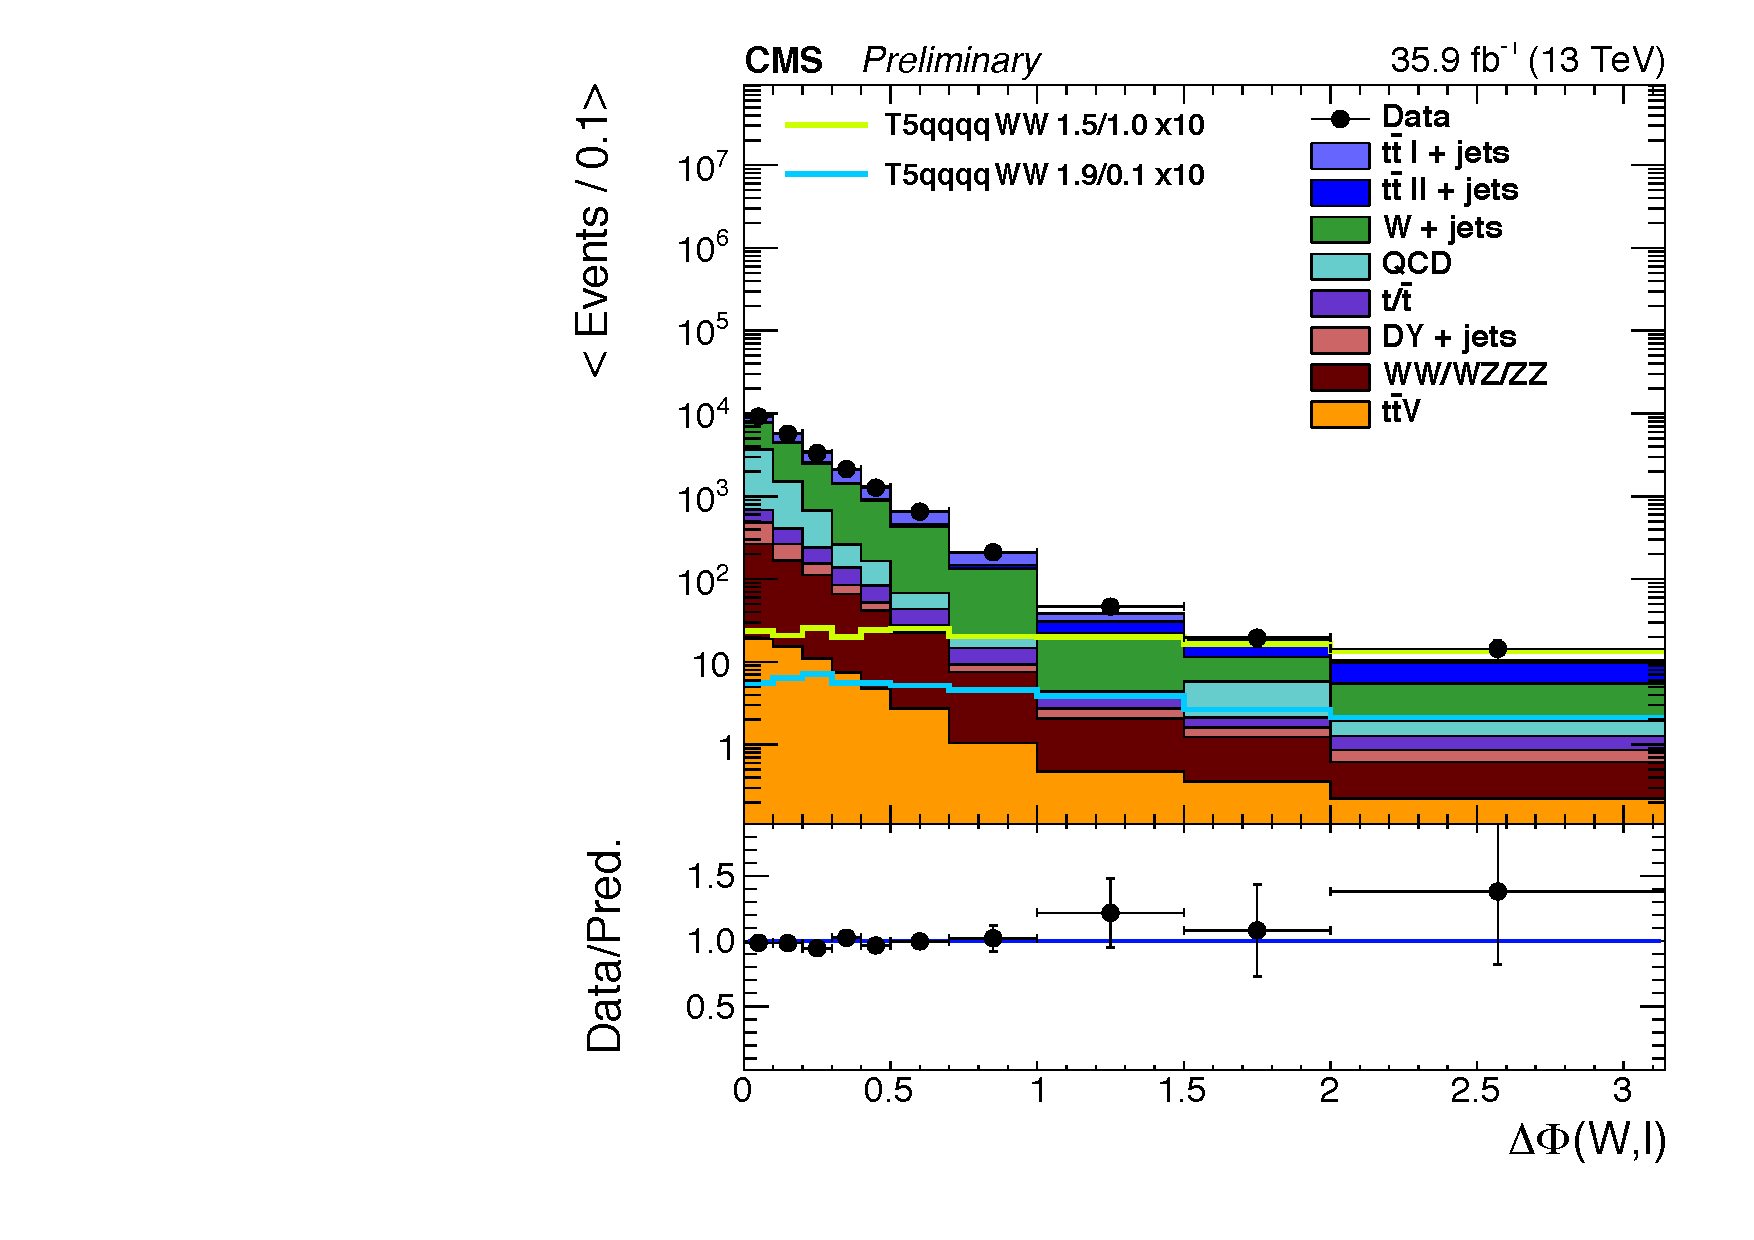
\includegraphics[width=0.45 \textwidth]{Plots/analysis/control_Plots/plots_zerob_st250_ht500_njet5_nbtagEq0_deltaPhi_WlPreliminary}
  \caption{ \label{fig:baselineplots} The top left distribution shows the number of b-tagged jets, after the baseline selection, requiring at least five jets, minimum $\HT$ of 500 GeV, a minimum $\LT$ of 250 GeV and exactly one lepton with $\pt >$25 GeV. The rest of the distributions are plotted after the same baseline selection additionally requiring no b-tagged jets. In the top row the number of jets (right) while in the bottom row $\HT$ (left) and $\LT$ (right) distributions are shown. The simulated background events are stacked on top of each other, and several signal points are overlaid for illustration without being stacked. The model T5qqqqWW (1.5,1.0) (T5qqqqWW (1.9,0.1)) corresponds to a gluino mass of 1.5 TeV (1.9 TeV) and neutralino mass of 1.1 TeV (0.1 TeV), respectively. The intermediate chargino mass is fixed at 1.25 TeV (1.0 TeV). The two benchmark signal models are scaled up by a factor of 10.
  }
   \end{center}
\end{figure*}
\chapter{Design of Search Regions}
Explain MB , SB...  
\newpage
\section{Signal Regions}
\subsection{Background and Signal composition in MB SR}
\newpage
\section{Control Regions}
\subsection{Background composition in MB CR and SB SR/CR}
\newpage
\newpage
\subsection{Signal contamination in MB CR and SB SR/CR}
Tell that It is negligible
\newpage

\chapter{Background Estimation}
\section{$R_{CS}$ method}
refer background compositions from the previous chapter 
\subsection{$R_{CS}$ method in ttbar events}
Maybe mention: Previously : SB was 1 bjet events -> you studied the extension now It is btagged region \\
Explain dilepton correction on kappa tt
\subsection{$R_{CS}$ method in w jets events}
\section{QCD background estimation}
keep short you did nothing 
\section{Validation of the background estimation}


\chapter{Systematic Uncertainties}

\chapter{Results and Interpretation}
\section{Results of background predition}
\newpage
\newpage
\section{Limit settings}
\newpage
\newpage
\section{Interpretation}
T5qqqqWW limit goes here
\section{Comparison to other results}
\newpage


\chapter{Conclusion}
Bitti
\newpage
The End
\newpage
Fin

\clearpage
%now enable appendix numbering format and include any appendices
\appendix
\chapter{MC Samples and cross sections}
\label{sec:Appsamples}

\begin{table}[htbp]
 \tiny
  \vspace{0.2cm}
  \begin{tabular}{|l|l|l|}
    \hline
    Sample name & Full name & cross section [pb] \\
    \hline
    TTJets\_SingleLeptonFromTbar & /TTJets\_SingleLeptFromTbar\_TuneCUETP8M1\_13TeV-madgraphMLM-pythia8 & 831.76*(3*0.108)*(1-3*0.108)  \\
    TTJets\_SingleLeptonFromTbar\_ext & /TTJets\_SingleLeptFromTbar\_TuneCUETP8M1\_13TeV-madgraphMLM-pythia8 & 831.76*(3*0.108)*(1-3*0.108)  \\
    TTJets\_SingleLeptonFromT & /TTJets\_SingleLeptFromT\_TuneCUETP8M1\_13TeV-madgraphMLM-pythia8 & 831.76*(3*0.108)*(1-3*0.108) \\
    TTJets\_SingleLeptonFromT\_ext & /TTJets\_SingleLeptFromT\_TuneCUETP8M1\_13TeV-madgraphMLM-pythia8 & 831.76*(3*0.108)*(1-3*0.108) \\
    TTJets\_DiLepton & /TTJets\_DiLept\_TuneCUETP8M1\_13TeV-madgraphMLM-pythia8 & 831.76*((3*0.108)**2)  \\
    TTJets\_DiLepton\_ext & /TTJets\_DiLept\_TuneCUETP8M1\_13TeV-madgraphMLM-pythia8 & 831.76*((3*0.108)**2)  \\
    TTJets\_LO\_HT600to800 & /TTJets\_HT-600to800\_TuneCUETP8M1\_13TeV-madgraphMLM-pythia8 & 1.610*831.76/502.2 \\
    TTJets\_LO\_HT600to800\_ext & /TTJets\_HT-600to800\_TuneCUETP8M1\_13TeV-madgraphMLM-pythia8 & 1.610*831.76/502.2 \\
    TTJets\_LO\_HT800to1200 & /TTJets\_HT-800to1200\_TuneCUETP8M1\_13TeV-madgraphMLM-pythia8 & 0.663*831.76/502.2 \\
    TTJets\_LO\_HT800to1200\_ext & /TTJets\_HT-800to1200\_TuneCUETP8M1\_13TeV-madgraphMLM-pythia8 & 0.663*831.76/502.2 \\
    TTJets\_LO\_HT1200to2500 & /TTJets\_HT-1200to2500\_TuneCUETP8M1\_13TeV-madgraphMLM-pythia8 & 0.12*831.76/502.2 \\
    TTJets\_LO\_HT1200to2500\_ext & /TTJets\_HT-1200to2500\_TuneCUETP8M1\_13TeV-madgraphMLM-pythia8 & 0.12*831.76/502.2 \\
    TTJets\_LO\_HT2500toInf & /TTJets\_HT-2500toInf\_TuneCUETP8M1\_13TeV-madgraphMLM-pythia8 & 0.001430*831.76/502.2 \\
    TTJets\_LO\_HT2500toInf\_ext & /TTJets\_HT-2500toInf\_TuneCUETP8M1\_13TeV-madgraphMLM-pythia8 & 0.001430*831.76/502.2 \\
     \hline
  \end{tabular}
  \caption{List of simulated $\ttJets$ background samples with a 25ns bunch crossing processed in CMSSW version 8\_0\_x.}
  \label{tab:ttsamples}
\end{table}

   \begin{table}[htbp]
  \tiny
  \vspace{0.2cm}
  \begin{tabular}{|l|l|l|}
    \hline
    Sample name & Full name & cross section [pb] \\
    \hline
      WJetsToLNu\_HT100to200 & /WJetsToLNu\_HT-100To200\_TuneCUETP8M1\_13TeV-madgraphMLM-pythia8 & 1345*1.21 \\
    WJetsToLNu\_HT100to200\_ext & /WJetsToLNu\_HT-100To200\_TuneCUETP8M1\_13TeV-madgraphMLM-pythia8 & 1345*1.21 \\
    WJetsToLNu\_HT200to400 & /WJetsToLNu\_HT-200To400\_TuneCUETP8M1\_13TeV-madgraphMLM-pythia8 & 359.7*1.21 \\
    WJetsToLNu\_HT200to400\_ext2 & /WJetsToLNu\_HT-200To400\_TuneCUETP8M1\_13TeV-madgraphMLM-pythia8 & 359.7*1.21 \\
    WJetsToLNu\_HT200to400\_ext & /WJetsToLNu\_HT-200To400\_TuneCUETP8M1\_13TeV-madgraphMLM-pythia8 & 359.7*1.21 \\
    WJetsToLNu\_HT400to600 & /WJetsToLNu\_HT-400To600\_TuneCUETP8M1\_13TeV-madgraphMLM-pythia8 & 48.91*1.21 \\
    WJetsToLNu\_HT400to600\_ext & /WJetsToLNu\_HT-400To600\_TuneCUETP8M1\_13TeV-madgraphMLM-pythia8 & 48.91*1.21 \\
    WJetsToLNu\_HT600to800 & /WJetsToLNu\_HT-600To800\_TuneCUETP8M1\_13TeV-madgraphMLM-pythia8 & 12.05*1.21 \\
    WJetsToLNu\_HT600to800\_ext & /WJetsToLNu\_HT-600To800\_TuneCUETP8M1\_13TeV-madgraphMLM-pythia8 & 12.05*1.21 \\
    WJetsToLNu\_HT800to1200 & /WJetsToLNu\_HT-800To1200\_TuneCUETP8M1\_13TeV-madgraphMLM-pythia8 & 5.501*1.21 \\
    WJetsToLNu\_HT800to1200\_ext & /WJetsToLNu\_HT-800To1200\_TuneCUETP8M1\_13TeV-madgraphMLM-pythia8 & 5.501*1.21 \\
    WJetsToLNu\_HT1200to2500 & /WJetsToLNu\_HT-1200To2500\_TuneCUETP8M1\_13TeV-madgraphMLM-pythia8 & 1.329*1.21 \\
    WJetsToLNu\_HT1200to2500\_ext & /WJetsToLNu\_HT-1200To2500\_TuneCUETP8M1\_13TeV-madgraphMLM-pythia8 & 1.329*1.21 \\
    WJetsToLNu\_HT2500toInf & /WJetsToLNu\_HT-2500ToInf\_TuneCUETP8M1\_13TeV-madgraphMLM-pythia8 & 0.03216*1.21 \\
    WJetsToLNu\_HT2500toInf\_ext & /WJetsToLNu\_HT-2500ToInf\_TuneCUETP8M1\_13TeV-madgraphMLM-pythia8 & 0.03216*1.21 \\
       \hline
  \end{tabular}
  \caption{List of simulated $\wJets$ background samples with a 25ns bunch crossing processed in CMSSW version 8\_0\_x.}
  \label{tab:Wsamples}
\end{table}  
   \begin{table}[htbp]
  \tiny
  \vspace{0.2cm}
  \begin{tabular}{|l|l|l|}
    \hline
    Sample name & Full name & cross section [pb] \\
    \hline
        TToLeptons\_sch & /ST\_s-channel\_4f\_leptonDecays\_13TeV-amcatnlo-pythia8\_TuneCUETP8M1 & (7.20+4.16)*0.108*3 \\
    T\_tch\_powheg & /ST\_t-channel\_top\_4f\_inclusiveDecays\_13TeV-powhegV2-madspin-pythia8\_TuneCUETP8M1 & 136.02 \\
    TBar\_tch\_powheg & /ST\_t-channel\_antitop\_4f\_inclusiveDecays\_13TeV-powhegV2-madspin-pythia8\_TuneCUETP8M1 & 80.95 \\
    TBar\_tWch\_ext1 & /ST\_tW\_antitop\_5f\_NoFullyHadronicDecays\_13TeV-powheg\_TuneCUETP8M1 & 19.55 \\
    TBar\_tWch\_ext2 & /ST\_tW\_antitop\_5f\_NoFullyHadronicDecays\_13TeV-powheg\_TuneCUETP8M1 & 19.55 \\
    TBar\_tWch & /ST\_tW\_antitop\_5f\_NoFullyHadronicDecays\_13TeV-powheg\_TuneCUETP8M1 & 19.55 \\
    T\_tWch\_ext1 & /ST\_tW\_top\_5f\_NoFullyHadronicDecays\_13TeV-powheg\_TuneCUETP8M1 & 19.55 \\
    T\_tWch\_ext2 & /ST\_tW\_top\_5f\_NoFullyHadronicDecays\_13TeV-powheg\_TuneCUETP8M1 & 19.55 \\
    T\_tWch & /ST\_tW\_top\_5f\_NoFullyHadronicDecays\_13TeV-powheg\_TuneCUETP8M1 & 19.55 \\
    DYJetsToLL\_M50\_HT100to200 & /DYJetsToLL\_M-50\_HT-100to200\_TuneCUETP8M1\_13TeV-madgraphMLM-pythia8 & 147.4*1.23 \\
    DYJetsToLL\_M50\_HT100to200\_ext & /DYJetsToLL\_M-50\_HT-100to200\_TuneCUETP8M1\_13TeV-madgraphMLM-pythia8 & 147.4*1.23 \\
    DYJetsToLL\_M50\_HT200to400 & /DYJetsToLL\_M-50\_HT-200to400\_TuneCUETP8M1\_13TeV-madgraphMLM-pythia8 & 40.99*1.23 \\
    DYJetsToLL\_M50\_HT200to400\_ext & /DYJetsToLL\_M-50\_HT-200to400\_TuneCUETP8M1\_13TeV-madgraphMLM-pythia8 & 40.99*1.23 \\
    DYJetsToLL\_M50\_HT400to600 & /DYJetsToLL\_M-50\_HT-400to600\_TuneCUETP8M1\_13TeV-madgraphMLM-pythia8 & 5.678*1.23 \\
    DYJetsToLL\_M50\_HT400to600\_ext & /DYJetsToLL\_M-50\_HT-400to600\_TuneCUETP8M1\_13TeV-madgraphMLM-pythia8 & 5.678*1.23 \\
    DYJetsToLL\_M50\_HT600to800 & /DYJetsToLL\_M-50\_HT-600to800\_TuneCUETP8M1\_13TeV-madgraphMLM-pythia8 & 1.367*1.23  \\
    DYJetsToLL\_M50\_HT800to1200 & /DYJetsToLL\_M-50\_HT-800to1200\_TuneCUETP8M1\_13TeV-madgraphMLM-pythia8 & 0.6304*1.23  \\
    DYJetsToLL\_M50\_HT1200to2500 & /DYJetsToLL\_M-50\_HT-1200to2500\_TuneCUETP8M1\_13TeV-madgraphMLM-pythia8 & 0.1514*1.23  \\
    DYJetsToLL\_M50\_HT2500toInf & /DYJetsToLL\_M-50\_HT-2500toInf\_TuneCUETP8M1\_13TeV-madgraphMLM-pythia8 & 0.003565*1.23  \\
    QCD\_HT300to500 & /QCD\_HT300to500\_TuneCUETP8M1\_13TeV-madgraphMLM-pythia8 & 351300 \\
    QCD\_HT300to500\_ext & /QCD\_HT300to500\_TuneCUETP8M1\_13TeV-madgraphMLM-pythia8 & 351300 \\
    QCD\_HT500to700 & /QCD\_HT500to700\_TuneCUETP8M1\_13TeV-madgraphMLM-pythia8 & 31630 \\
    QCD\_HT500to700\_ext & /QCD\_HT500to700\_TuneCUETP8M1\_13TeV-madgraphMLM-pythia8 & 31630 \\
    QCD\_HT700to1000 & /QCD\_HT700to1000\_TuneCUETP8M1\_13TeV-madgraphMLM-pythia8 & 6802 \\
    QCD\_HT700to1000\_ext & /QCD\_HT700to1000\_TuneCUETP8M1\_13TeV-madgraphMLM-pythia8 & 6802 \\
    QCD\_HT1000to1500 & /QCD\_HT1000to1500\_TuneCUETP8M1\_13TeV-madgraphMLM-pythia8 & 1206 \\
    QCD\_HT1000to1500\_ext & /QCD\_HT1000to1500\_TuneCUETP8M1\_13TeV-madgraphMLM-pythia8 & 1206 \\
    QCD\_HT1500to2000 & /QCD\_HT1500to2000\_TuneCUETP8M1\_13TeV-madgraphMLM-pythia8 & 120.4 \\
    QCD\_HT1500to2000\_ext & /QCD\_HT1500to2000\_TuneCUETP8M1\_13TeV-madgraphMLM-pythia8 & 120.4 \\
    QCD\_HT2000toInf & /QCD\_HT2000toInf\_TuneCUETP8M1\_13TeV-madgraphMLM-pythia8 & 25.25 \\
    QCD\_HT2000toInf\_ext & /QCD\_HT2000toInf\_TuneCUETP8M1\_13TeV-madgraphMLM-pythia8 & 25.25 \\
    WWTo2L2Nu & /WWTo2L2Nu\_13TeV-powheg & 10.481  \\
    WWToLNuQQ & /WWToLNuQQ\_13TeV-powheg & 43.53  \\
    WWToLNuQQ\_ext & /WWToLNuQQ\_13TeV-powheg & 43.53  \\
    ZZTo2L2Nu & /ZZTo2L2Nu\_13TeV\_powheg\_pythia8 & 0.564 \\
    ZZTo2L2Q & /ZZTo2L2Q\_13TeV\_amcatnloFXFX\_madspin\_pythia8 & 3.28 \\
    ZZTo2Q2Nu & /ZZTo2Q2Nu\_13TeV\_amcatnloFXFX\_madspin\_pythia8 & 4.04 \\
    ZZTo2L2Nu & /ZZTo2L2Nu\_13TeV\_powheg\_pythia8 & 0.564 \\
    WZTo1L3Nu & /WZTo1L3Nu\_13TeV\_amcatnloFXFX\_madspin\_pythia8 & (47.13)*(3*0.108)*(0.2)  \\
    WZTo1L1Nu2Q & /WZTo1L1Nu2Q\_13TeV\_amcatnloFXFX\_madspin\_pythia8 & 10.71 \\
    WZTo2L2Q & /WZTo2L2Q\_13TeV\_amcatnloFXFX\_madspin\_pythia8 & 5.60 \\
    WWDouble & /WWTo2L2Nu\_DoubleScattering\_13TeV-pythia8 & 1.64 \\
    TTWToLNu\_ext & /TTWJetsToLNu\_TuneCUETP8M1\_13TeV-amcatnloFXFX-madspin-pythia8 & 0.2043 \\
    TTWToLNu\_ext2 & /TTWJetsToLNu\_TuneCUETP8M1\_13TeV-amcatnloFXFX-madspin-pythia8 & 0.2043 \\
    TTWToQQ & /TTWJetsToQQ\_TuneCUETP8M1\_13TeV-amcatnloFXFX-madspin-pythia8 & 0.40620 \\
    TTZToQQ & /TTZToQQ\_TuneCUETP8M1\_13TeV-amcatnlo-pythia8 & 0.5297 \\
    TTZToLLNuNu & /TTZToLLNuNu\_M-10\_TuneCUETP8M1\_13TeV-amcatnlo-pythia8 & 0.2529 \\
    TTZToLLNuNu\_m1to10 & /TTZToLL\_M-1to10\_TuneCUETP8M1\_13TeV-madgraphMLM-pythia8 & 0.0493 \\
    \hline
  \end{tabular}
  \caption{List of the rest of simulated background samples with a 25ns bunch crossing processed in CMSSW version 8\_0\_x.}
  \label{tab:samples}
\end{table}

\chapter{Control Plots}
\label{sec:CRplots}

Figures~\ref{fig:0bmu_zeroB_3_4jets_CR} to \ref{fig:0bele_0p5_CR} show distributions of observables in sidebands at low \njet, separately for electrons and muons.
Figures~\ref{fig:0bmu_zeroB_3_4jets_CR} and \ref{fig:0bele_zeroB_3_4jets_CR} present the sideband defined by $\ST>250\GeV$, $\HT>500\GeV$, and $3\leq\njet\leq4$, used in the estimation of the \wJets background.
Figures~\ref{fig:0bmu_1B_4_5jets_CR} and \ref{fig:0bele_1B_4_5jets_CR} show the sideband defined by $\ST>250\GeV$, $\HT>500\GeV$, $\nbjet\geq1$, and $4\leq\njet\leq5$, used in the estimation of the \ttJets background.
Distributions in the mainband are shown in Figures~\ref{fig:0bmu_0p5_CR} and \ref{fig:0bele_0p5_CR}.

\begin{figure}[p]
  \begin{center}
    \subfigure[\njet]{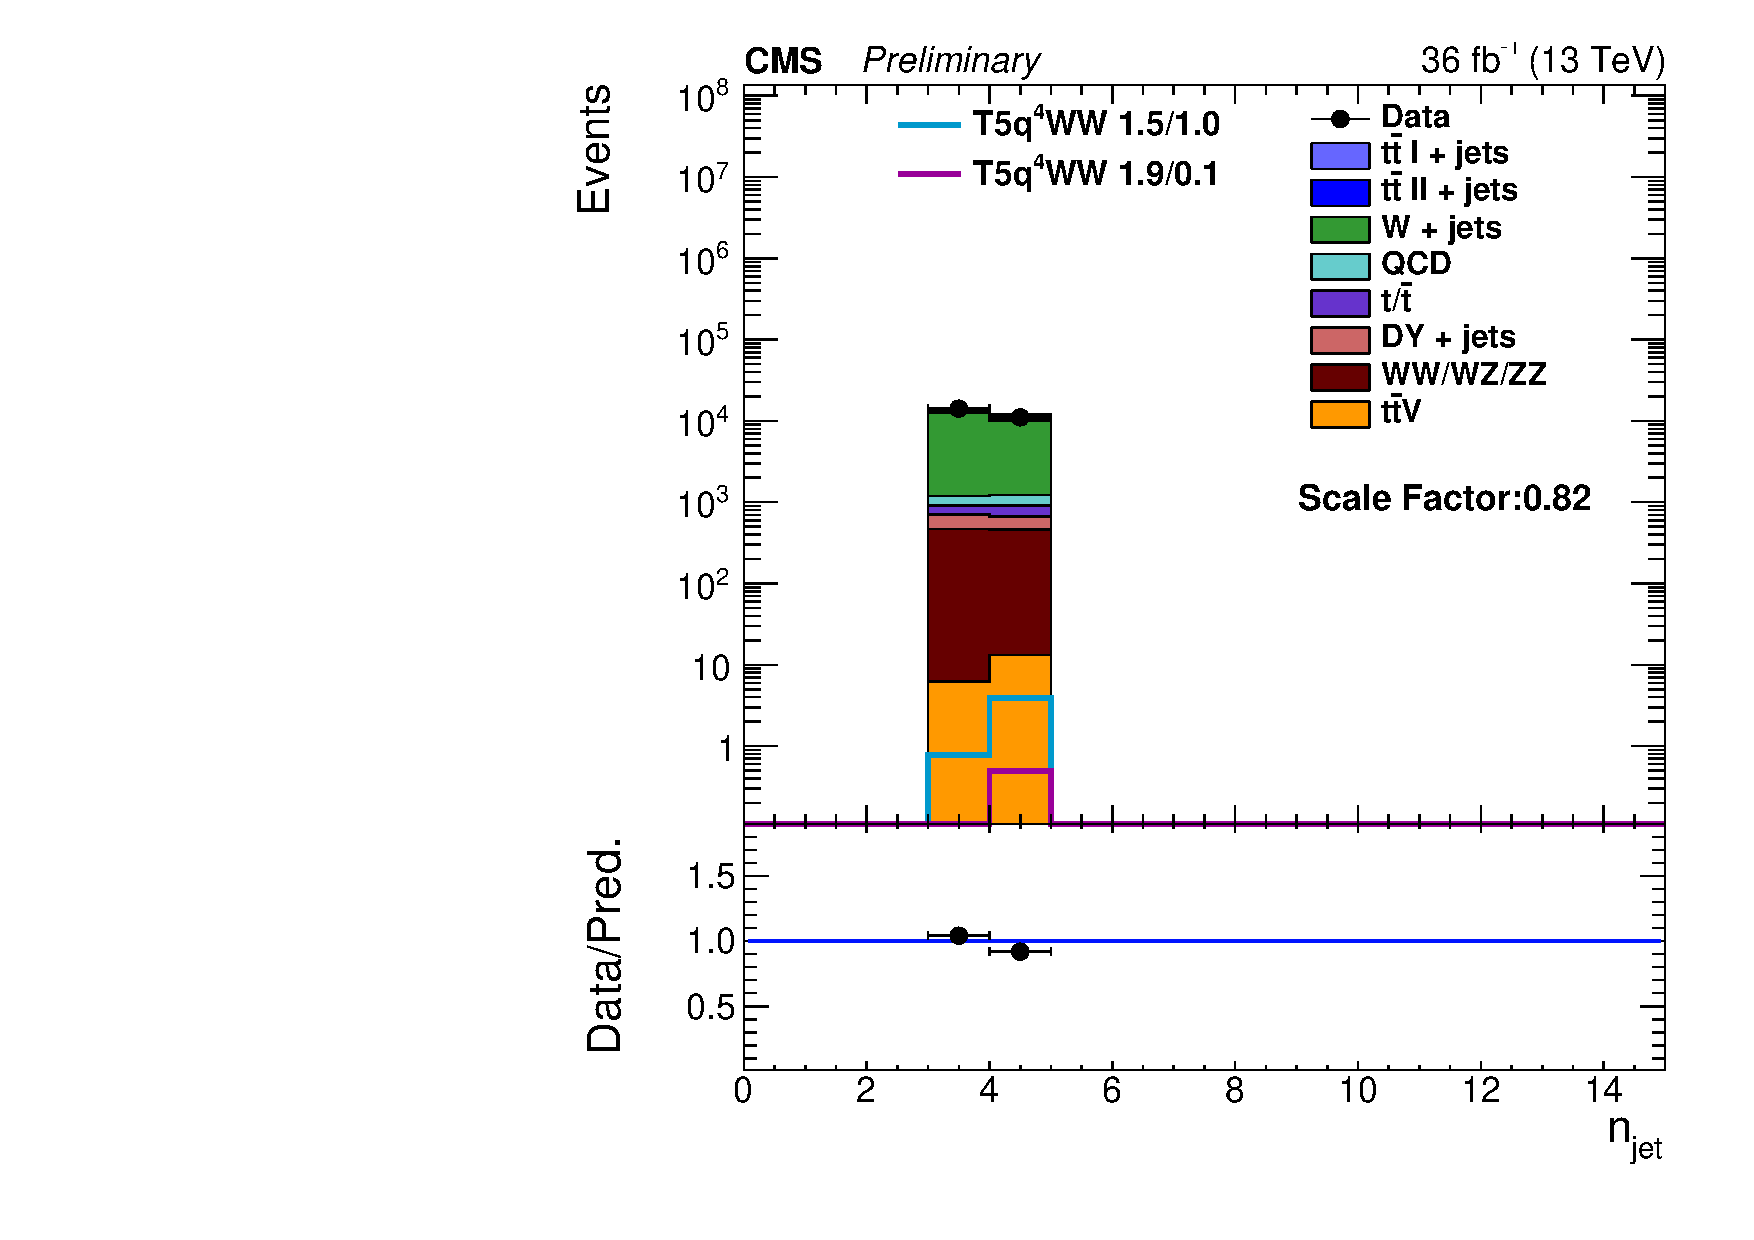
\includegraphics[angle=0,width=.32\textwidth]                  {Plots//analysis/control_Plots/mu/st250_ht500_njet3-4_nbtagEq0/nJet30.pdf}}
    \subfigure[$p_T(\textrm{1st jet})$]{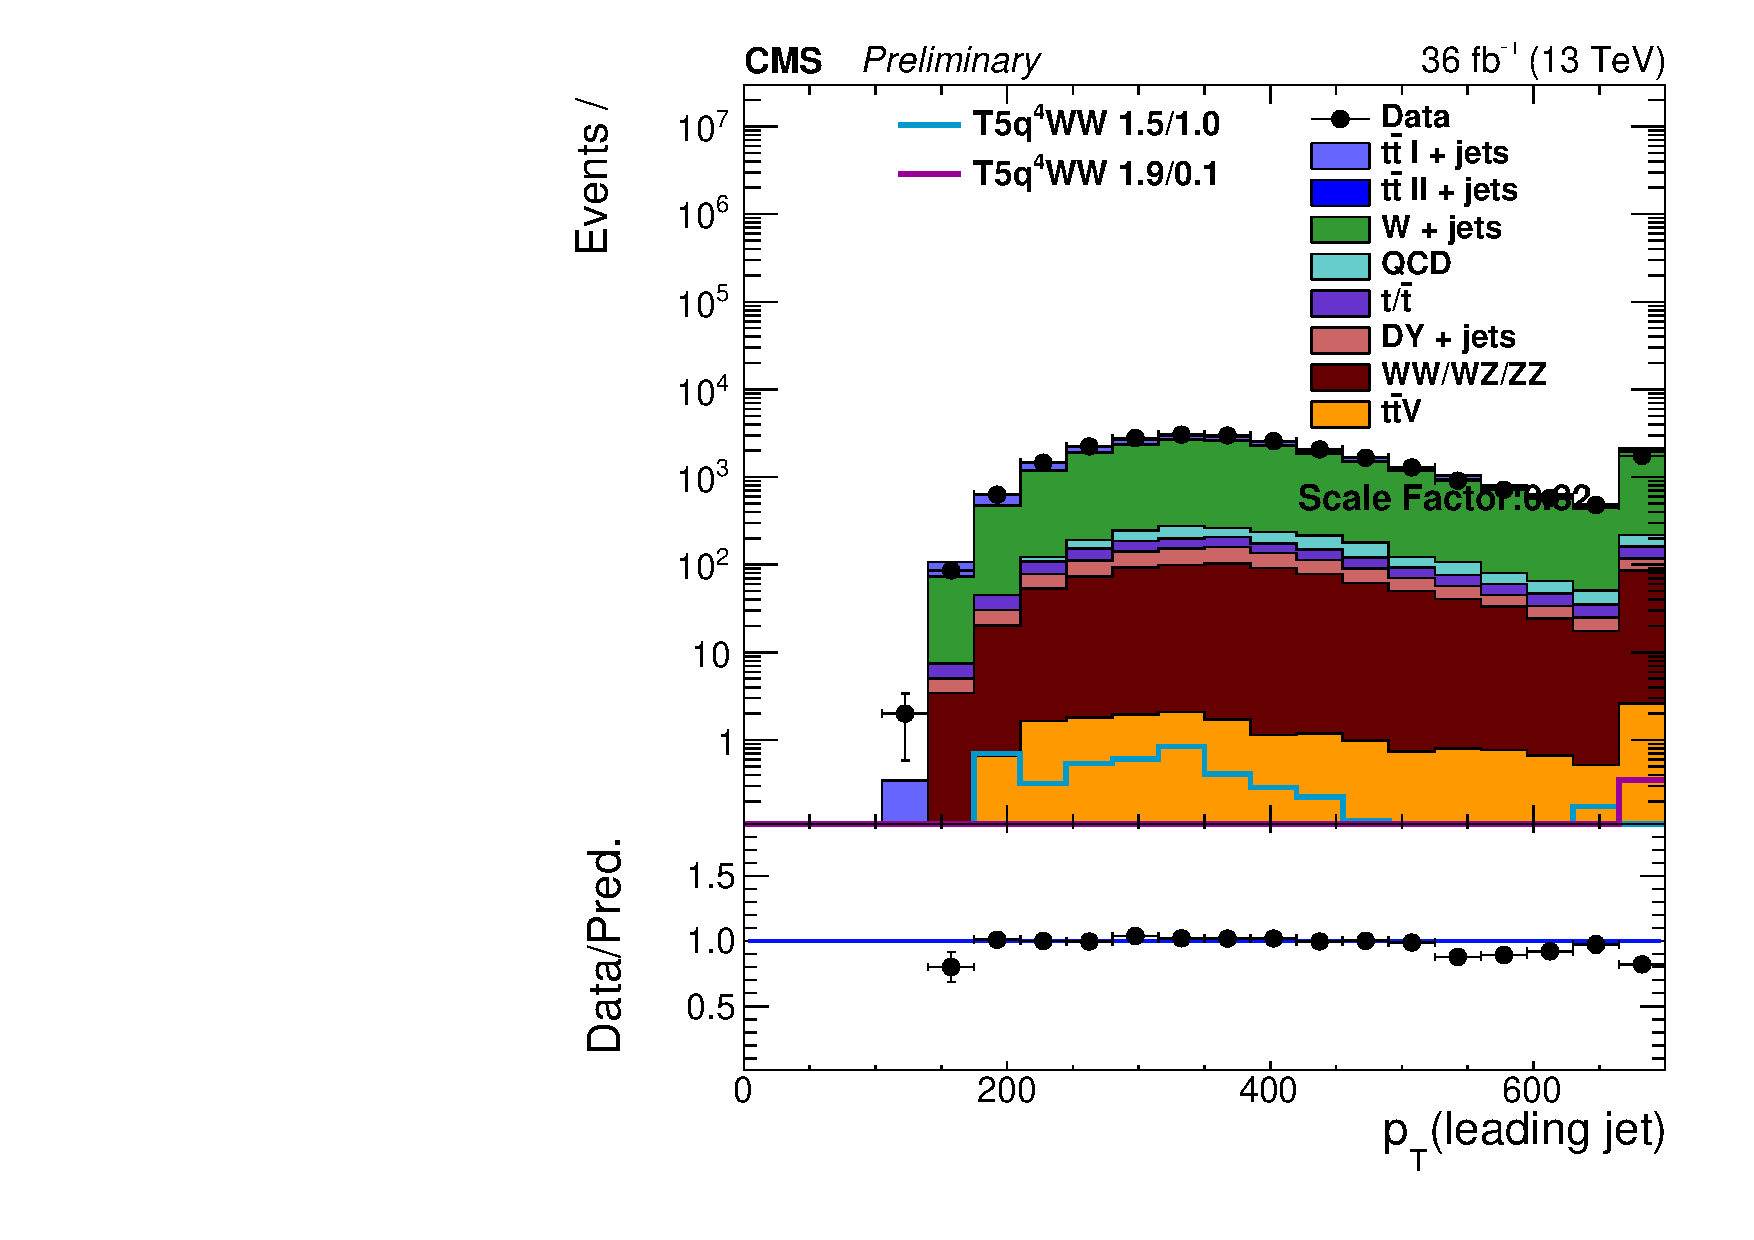
\includegraphics[angle=0,width=.32\textwidth]{Plots//analysis/control_Plots/mu/st250_ht500_njet3-4_nbtagEq0/leading_JetPt.pdf}}
    \subfigure[$n_{\textrm{vertex}}$]{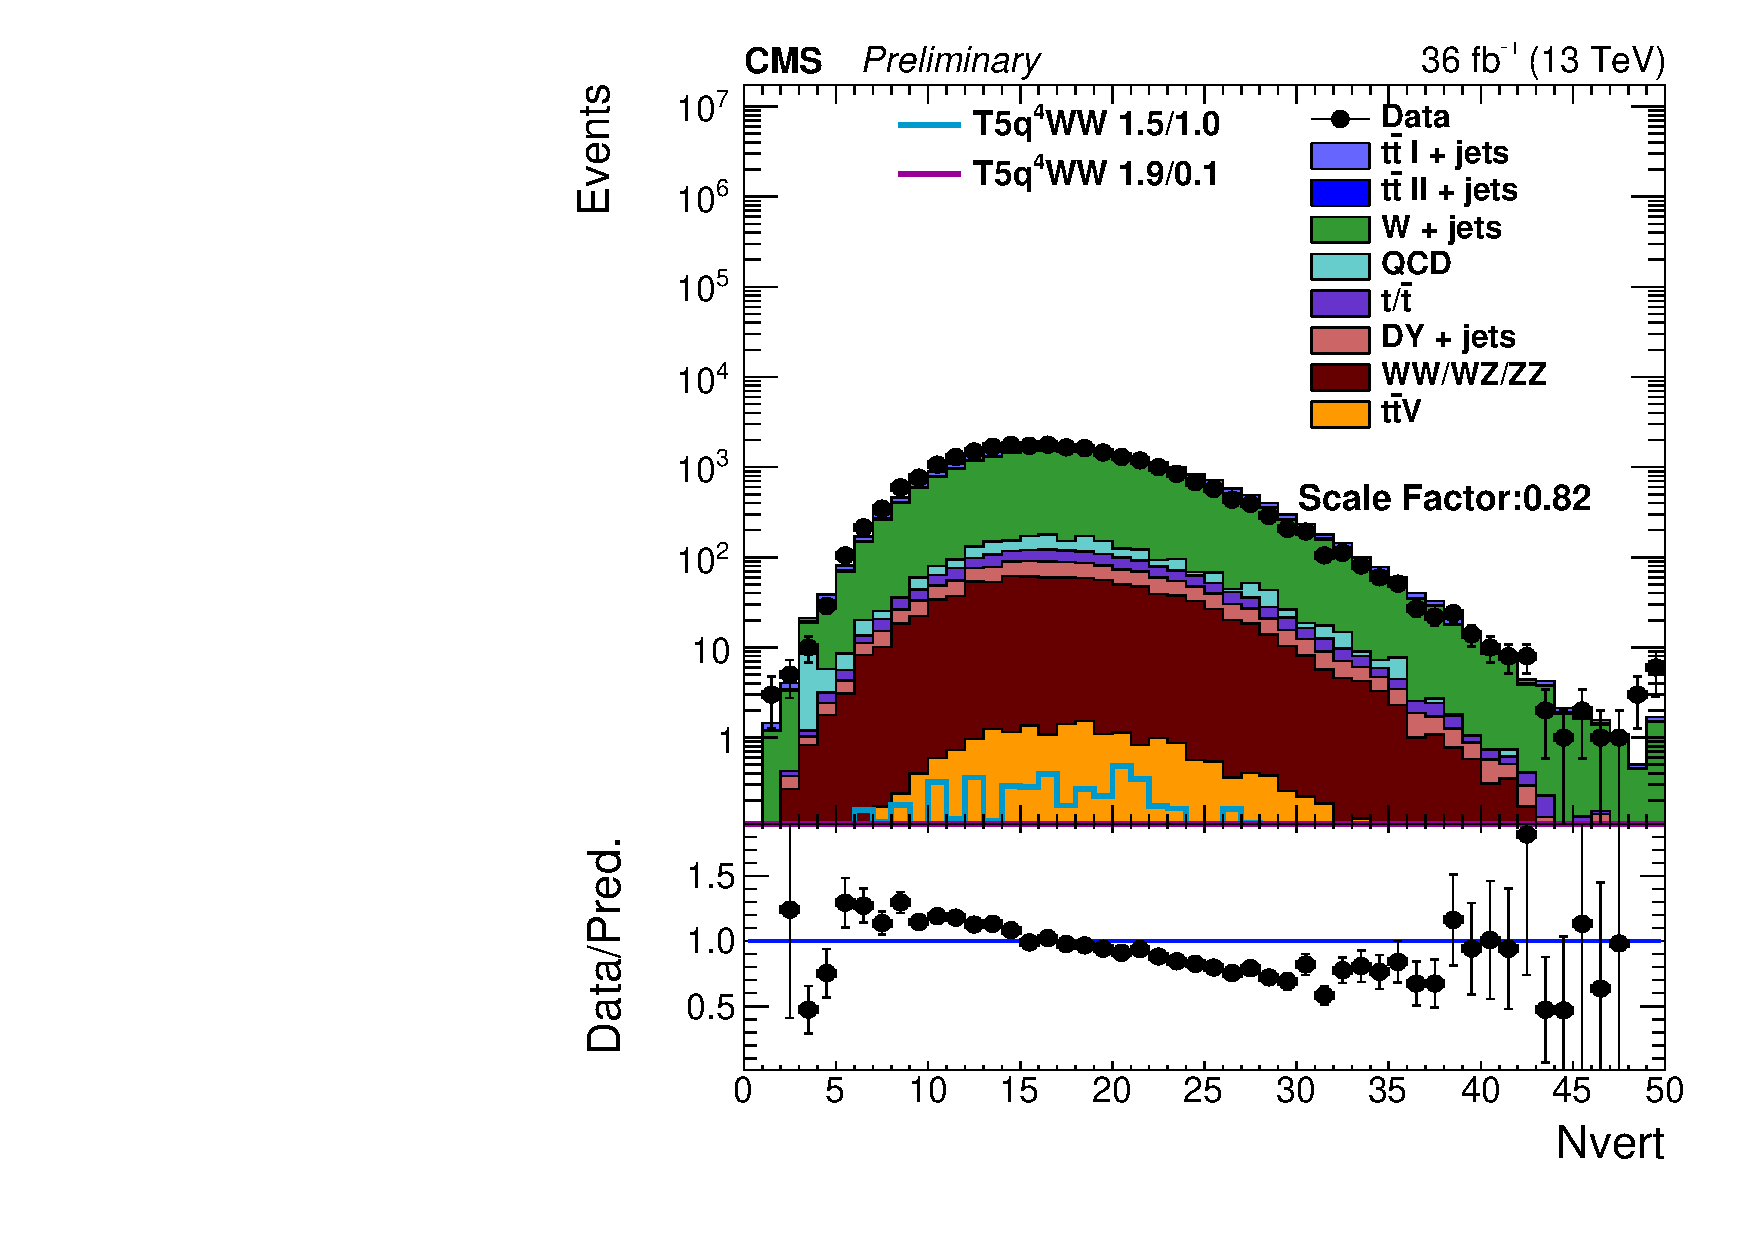
\includegraphics[angle=0,width=.32\textwidth]       {Plots//analysis/control_Plots/mu/st250_ht500_njet3-4_nbtagEq0/nVert.pdf}}\\
    \subfigure[$p_T(l)$]{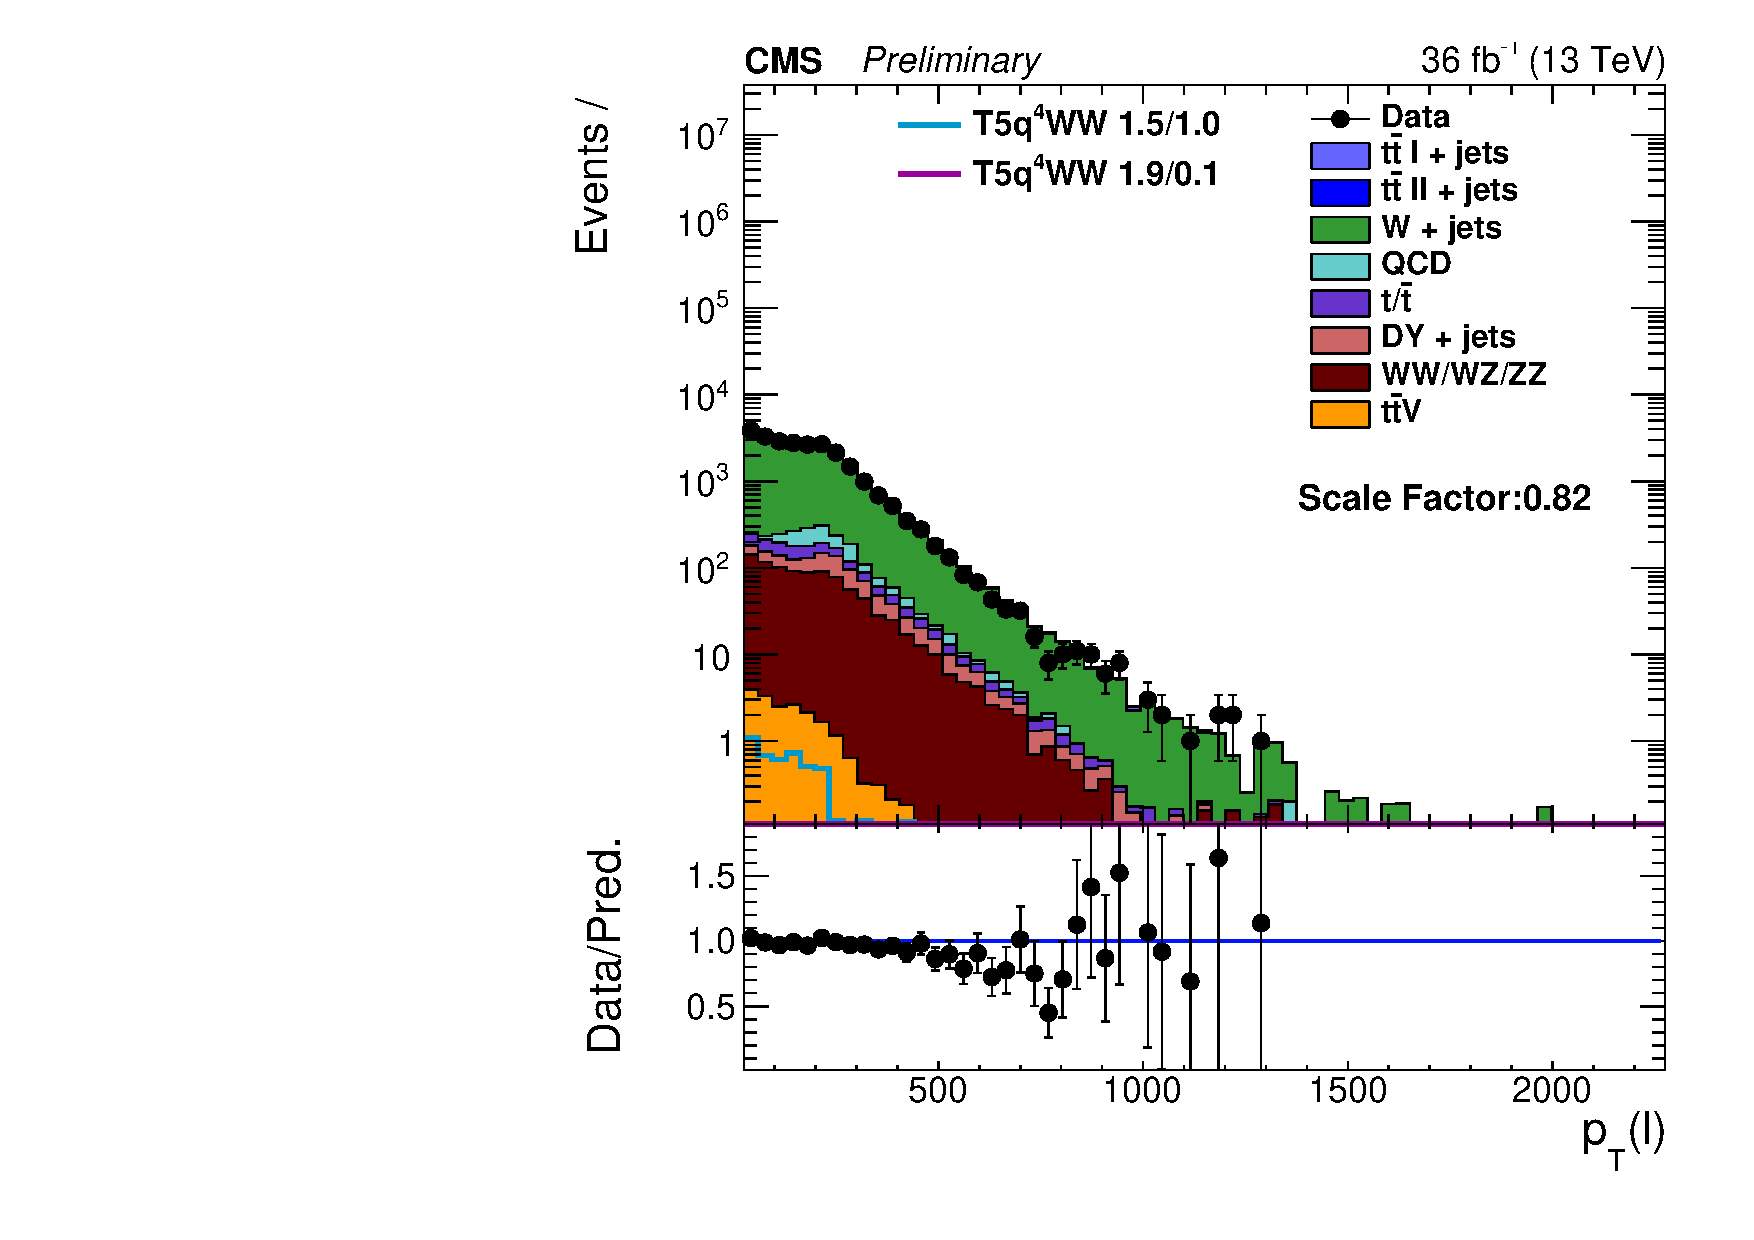
\includegraphics[angle=0,width=.32\textwidth]               {Plots//analysis/control_Plots/mu/st250_ht500_njet3-4_nbtagEq0/leptonPt.pdf}}
    \subfigure[$m_{T2}$]{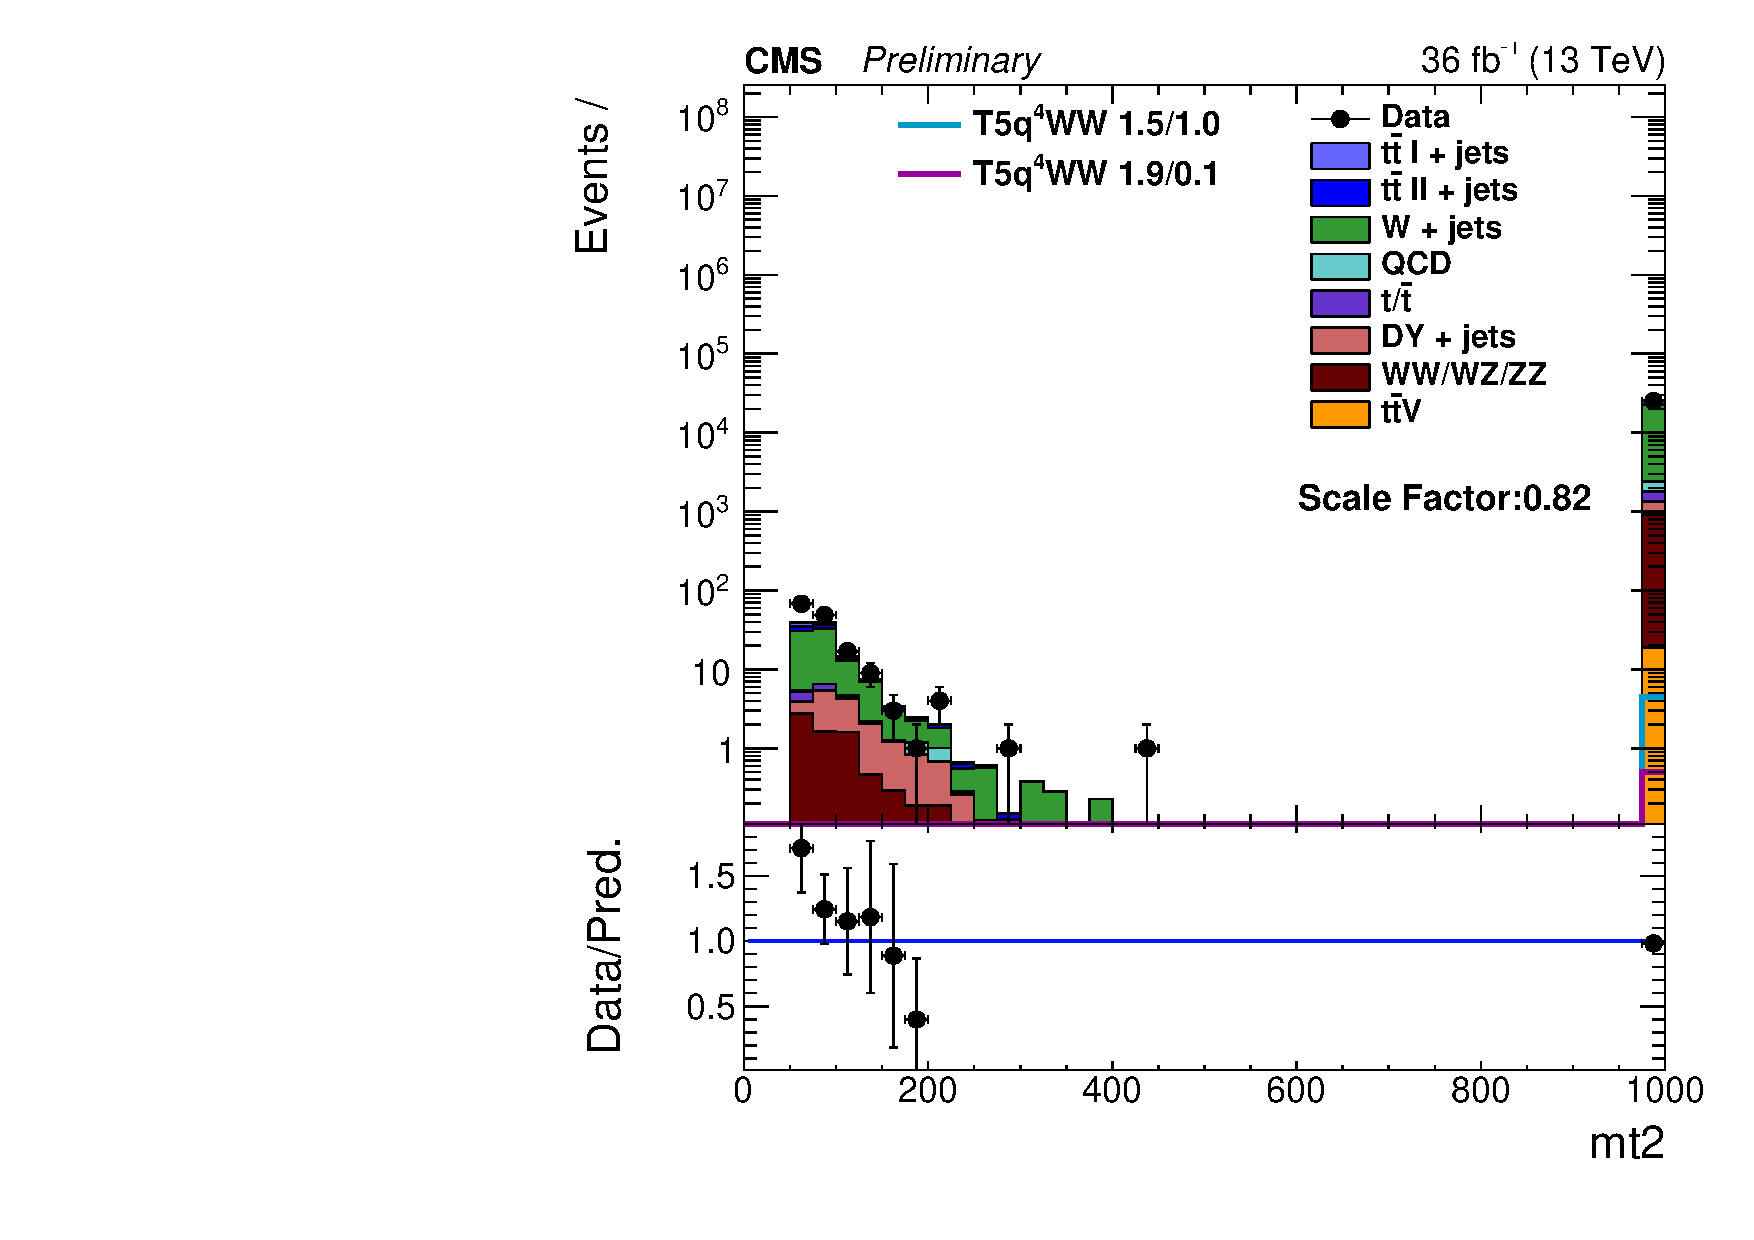
\includegraphics[angle=0,width=.32\textwidth]              {Plots//analysis/control_Plots/mu/st250_ht500_njet3-4_nbtagEq0/iso_MT2.pdf}}
    \subfigure[miniIsolation$(l)$]{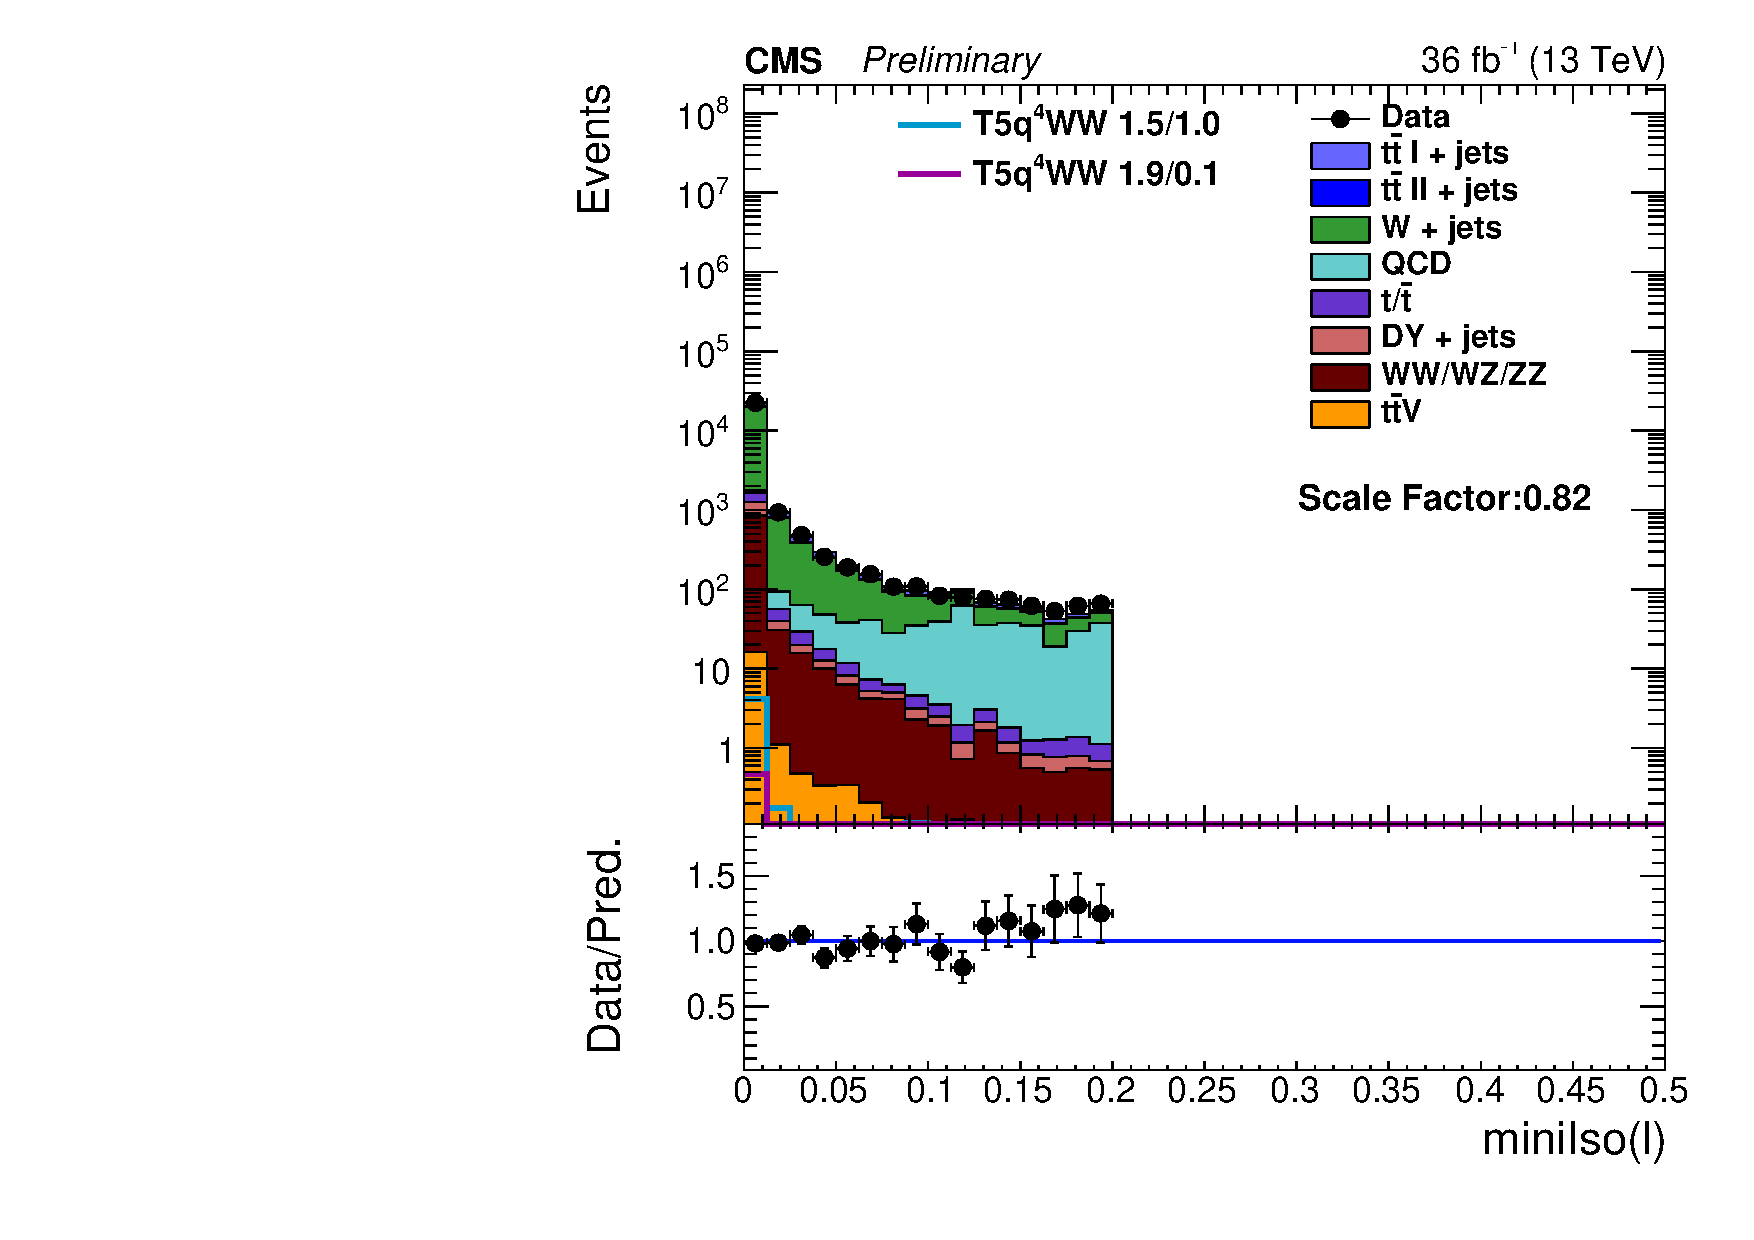
\includegraphics[angle=0,width=.32\textwidth]     {Plots//analysis/control_Plots/mu/st250_ht500_njet3-4_nbtagEq0/leptonminiIso.pdf}}\\
    \subfigure[\HT]{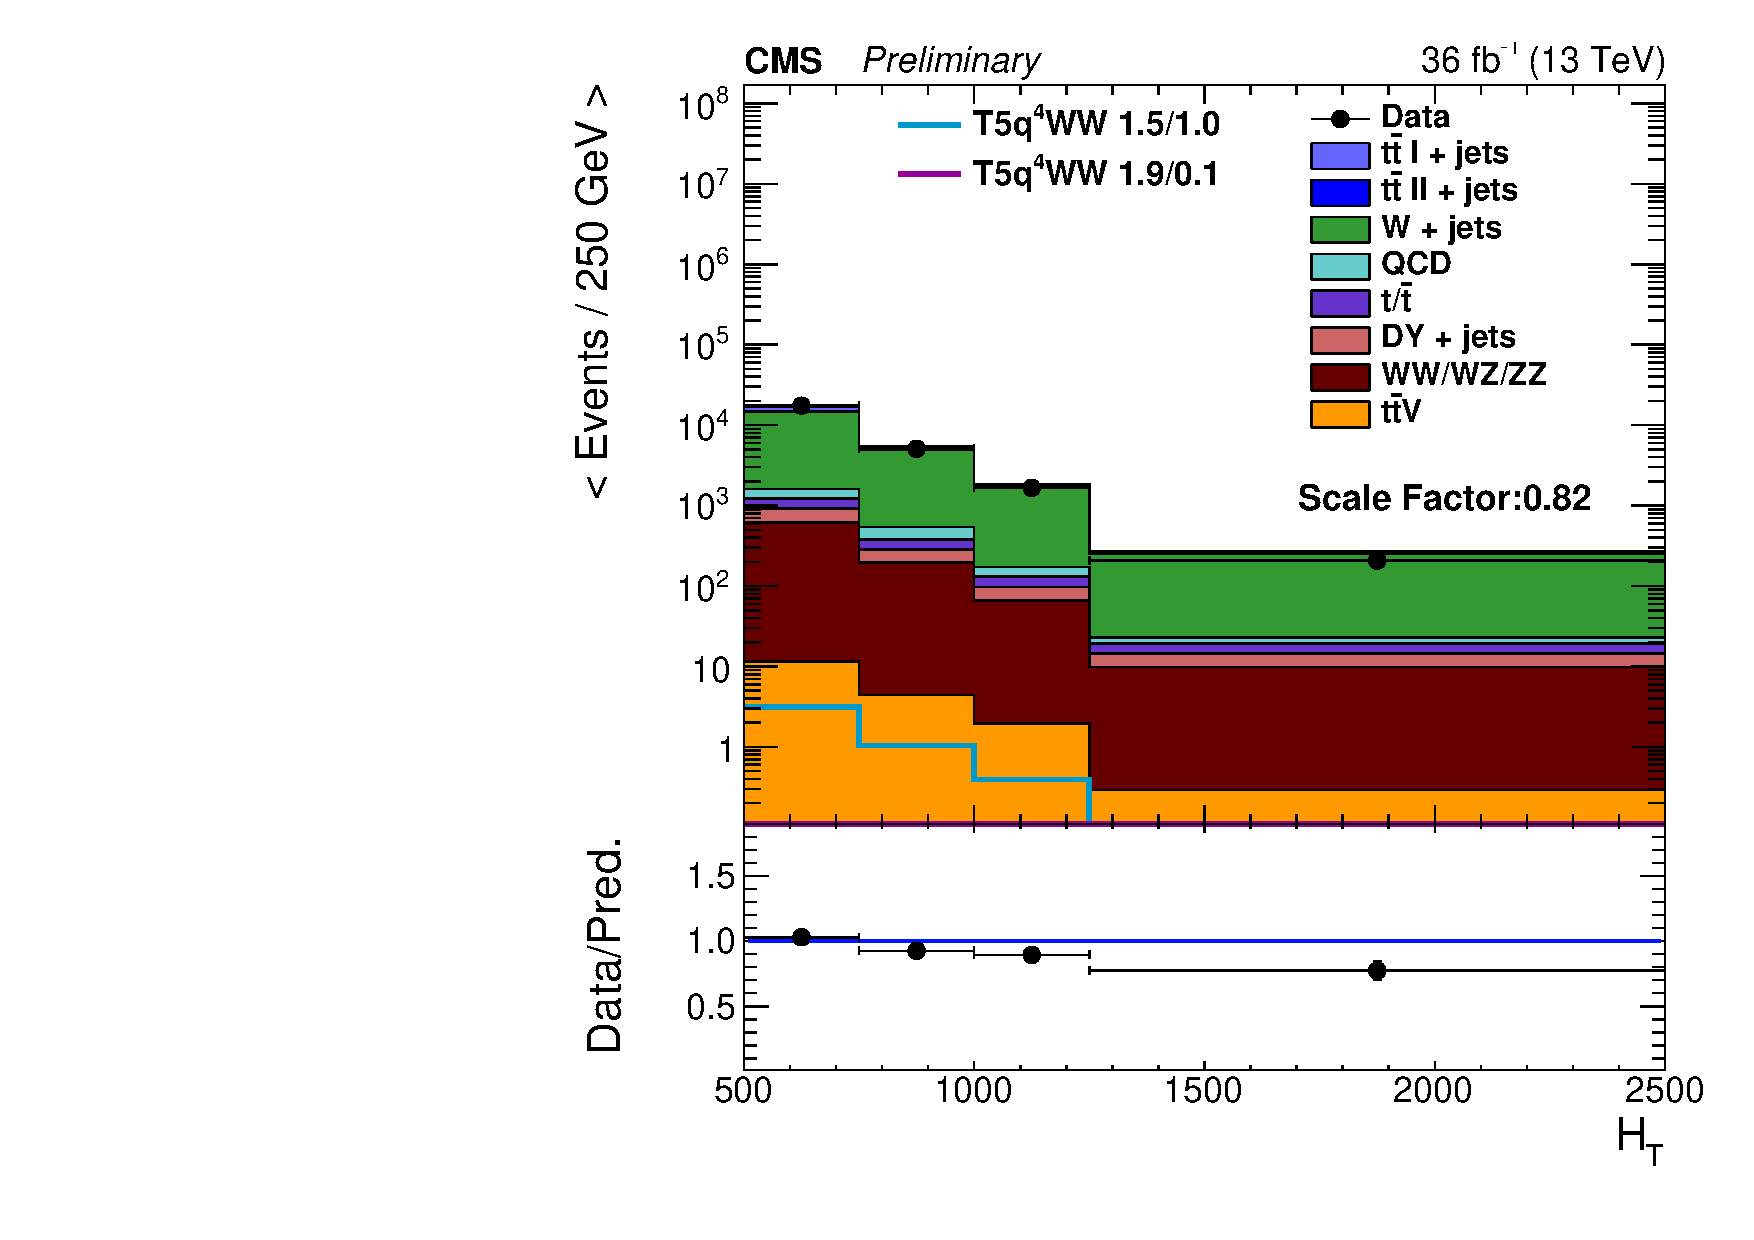
\includegraphics[angle=0,width=.32\textwidth]                    {Plots//analysis/control_Plots/mu/st250_ht500_njet3-4_nbtagEq0/htJet30j.pdf}}
    \subfigure[\LT]{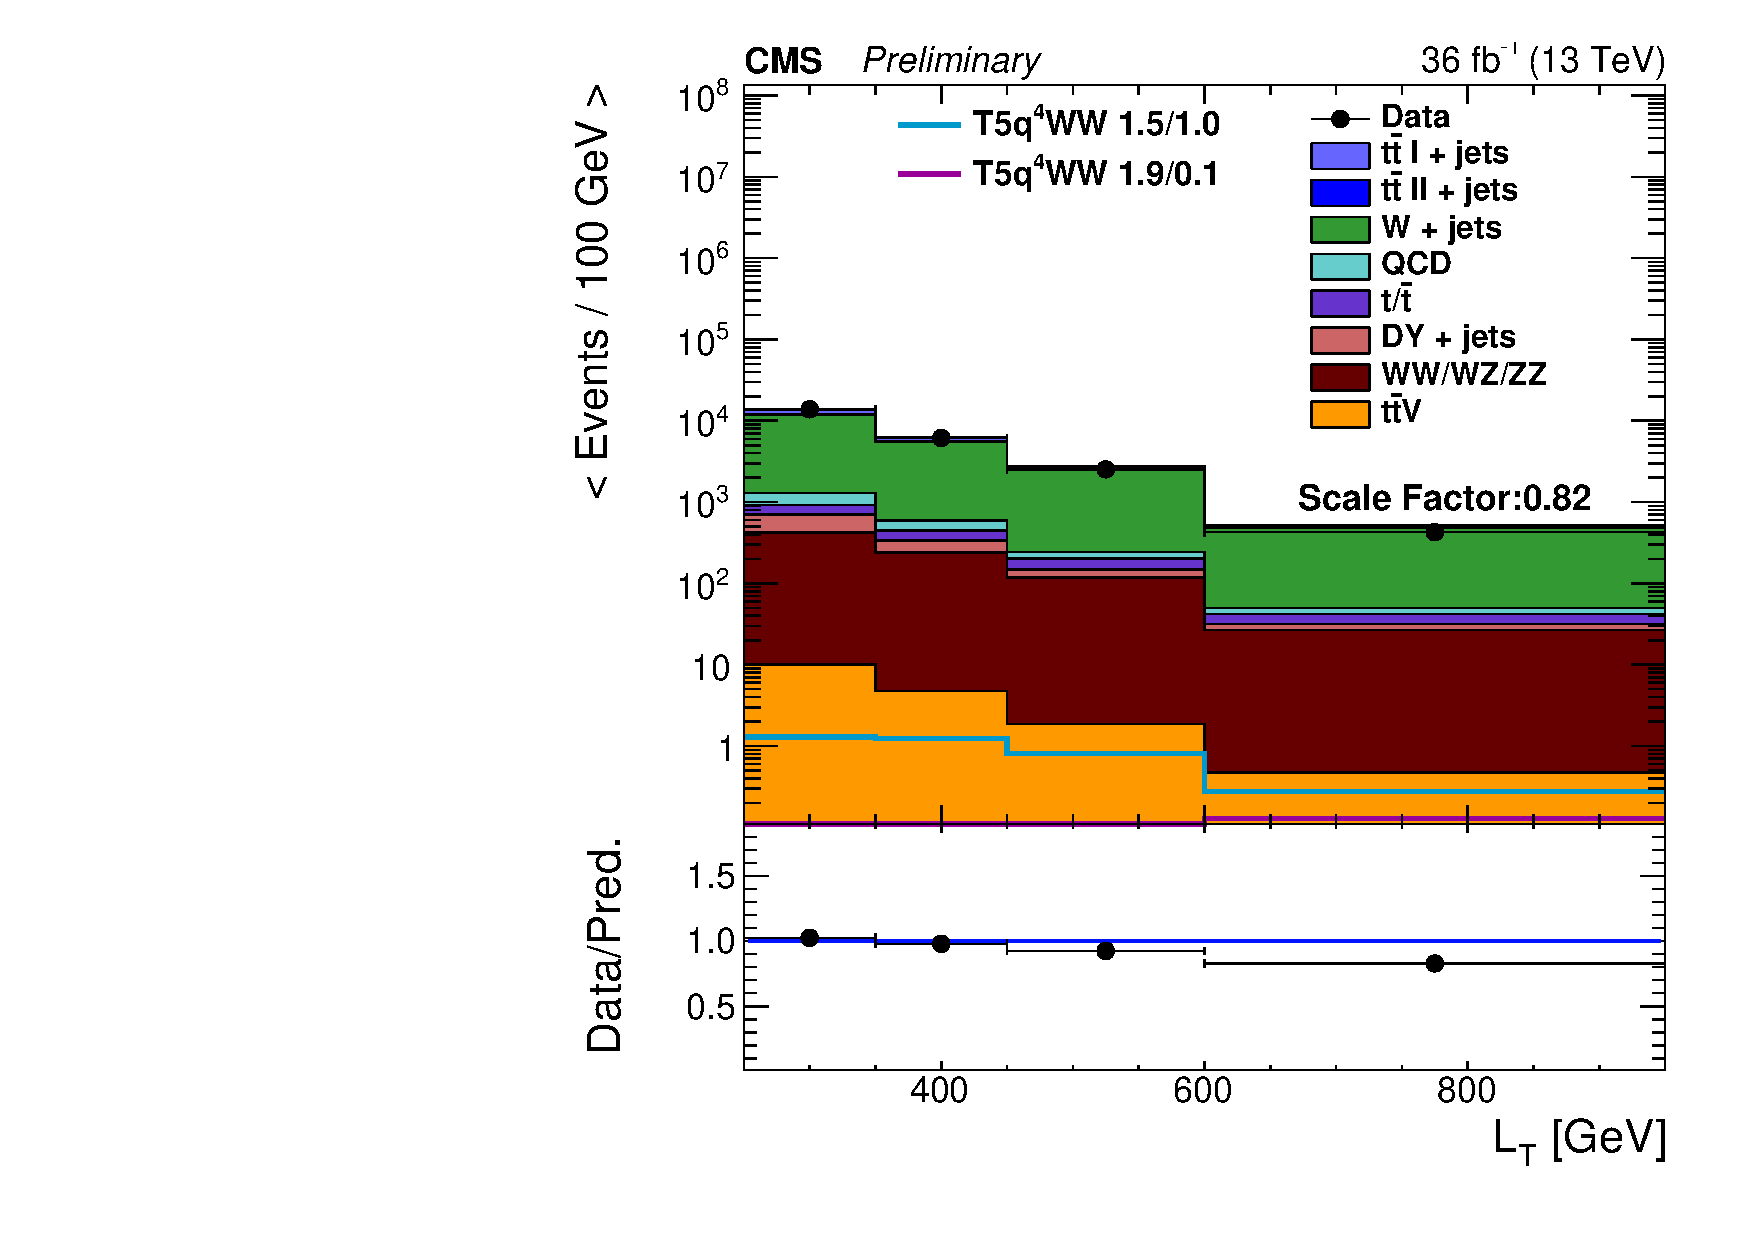
\includegraphics[angle=0,width=.32\textwidth]                    {Plots//analysis/control_Plots/mu/st250_ht500_njet3-4_nbtagEq0/LT.pdf}}
    \subfigure[\DF]{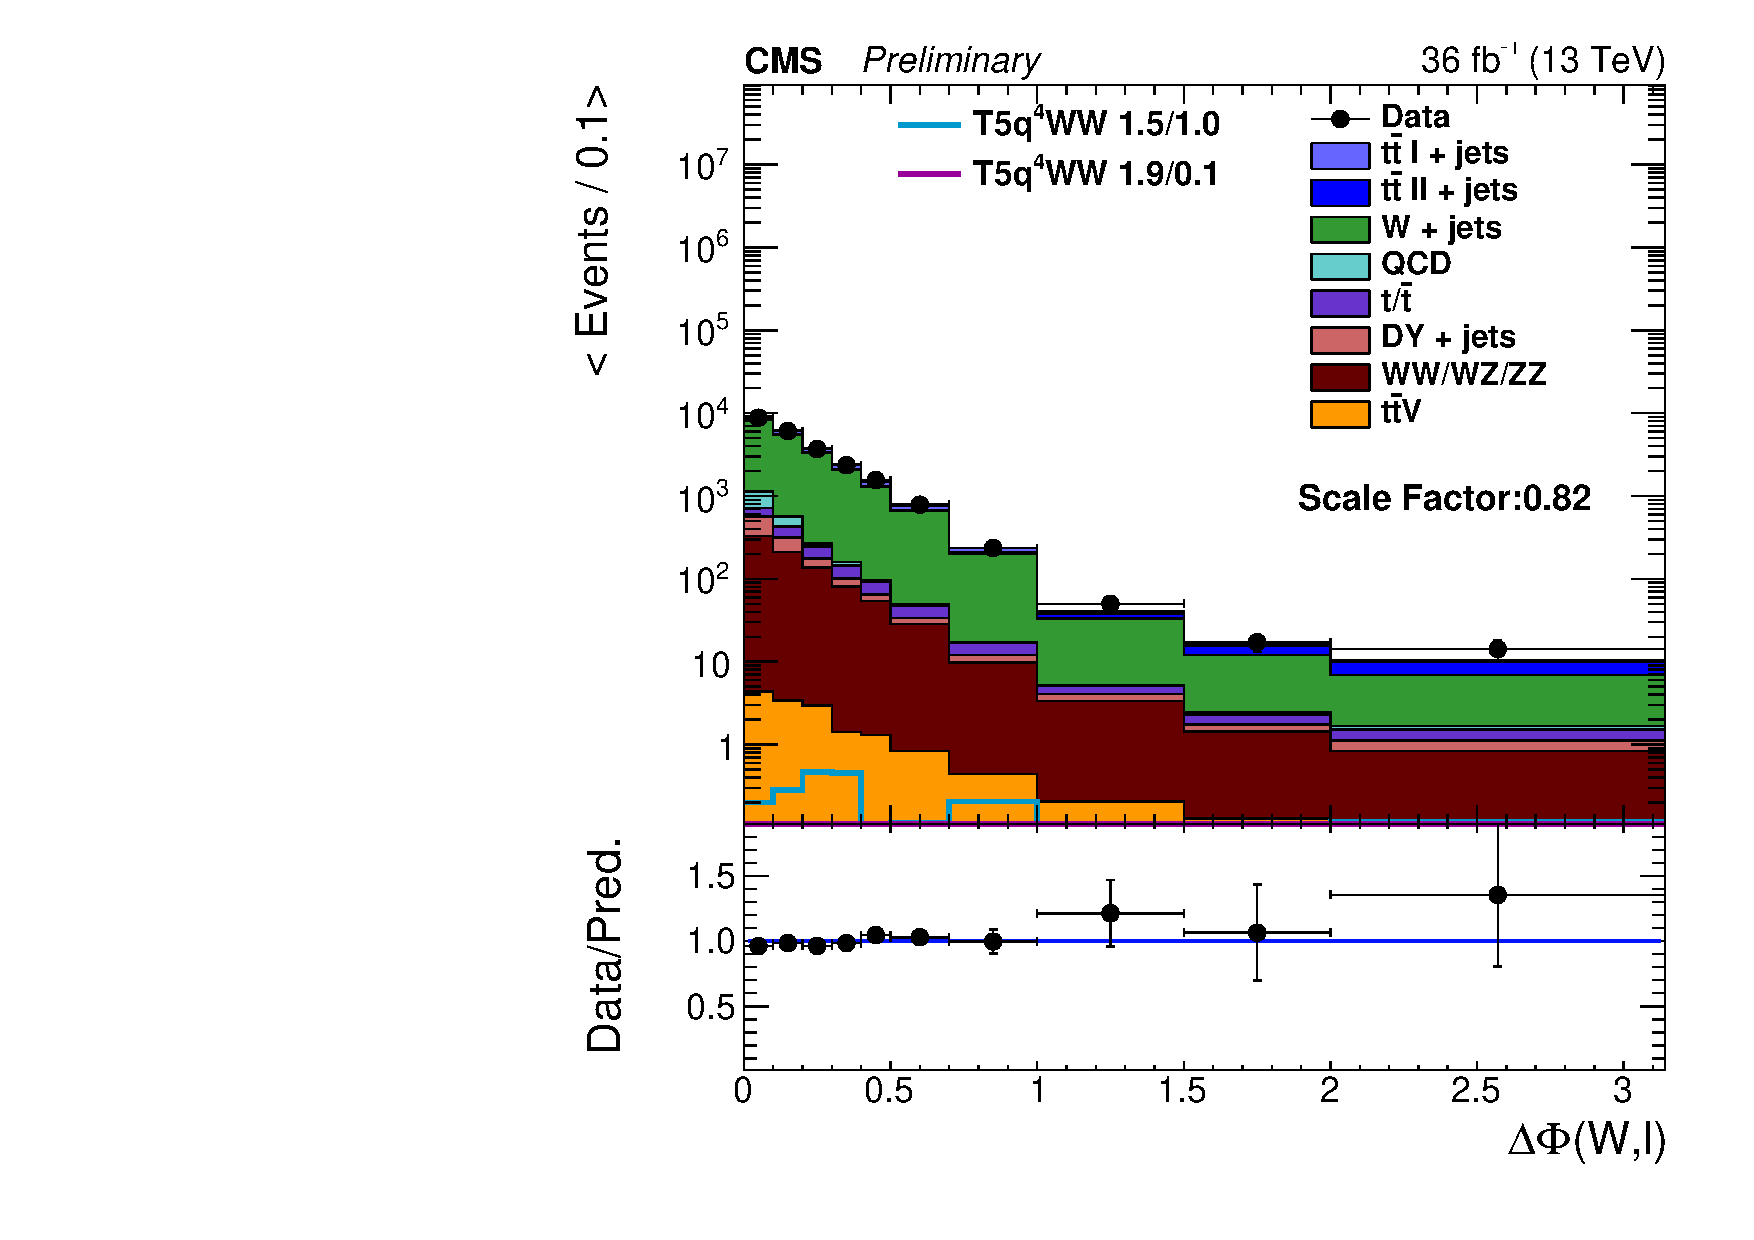
\includegraphics[angle=0,width=.32\textwidth]                    {Plots//analysis/control_Plots/mu/st250_ht500_njet3-4_nbtagEq0/deltaPhi_Wl.pdf}}

    \caption{Distribution of kinematic observables after requiring $\HT >$ 500 \GeV, $\LT >$ 250 \GeV, $3\leq$ jets $\leq4$  and zero b-tagged jets (1 $\mu$ channel).
      %In order to blind the signal region, data events with large \DF (corresponding to the dynamic \DF cut) are excluded from the \DF plot.
    }
    \label{fig:0bmu_zeroB_3_4jets_CR}
  \end{center}
\end{figure}



\begin{figure}[p]
  \begin{center}
    \subfigure[\njet]{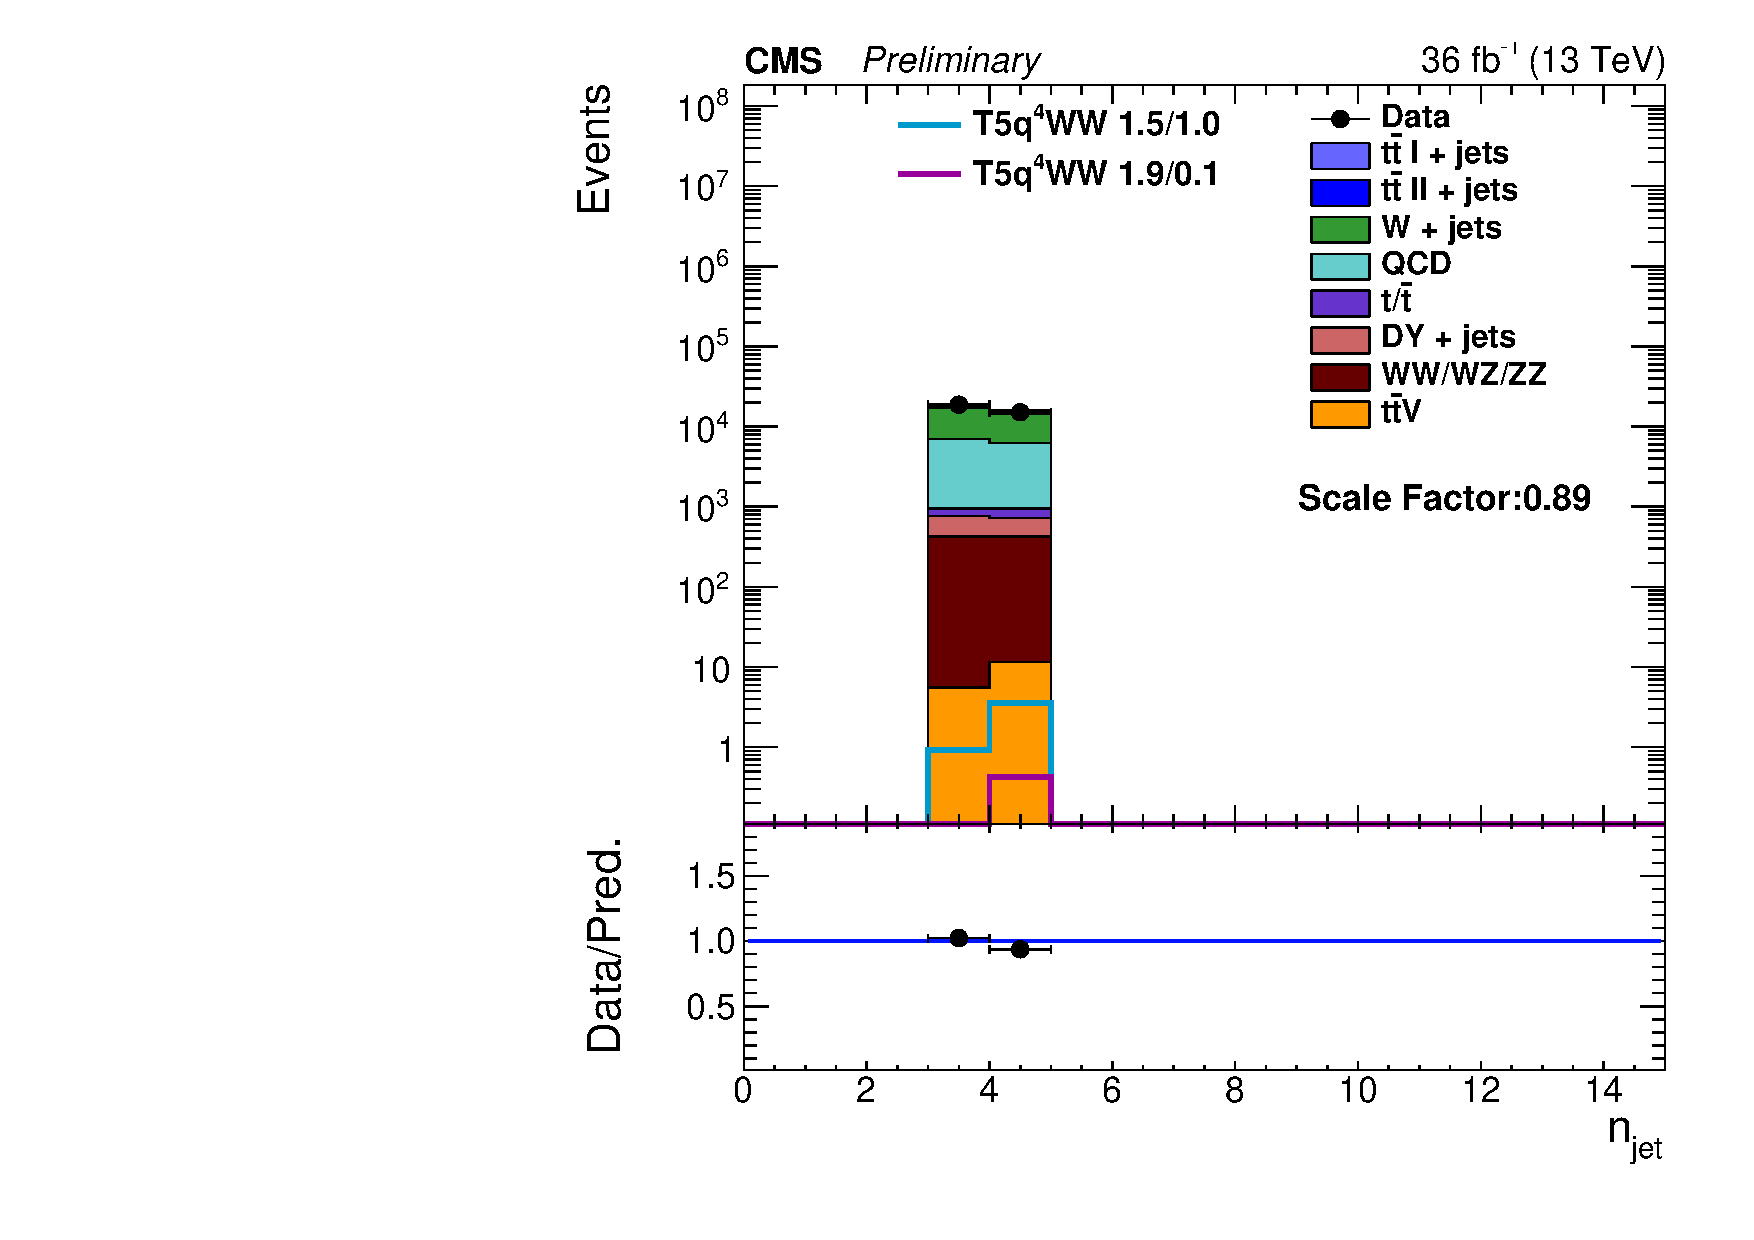
\includegraphics[angle=0,width=.32\textwidth]                  {Plots//analysis/control_Plots/ele/st250_ht500_njet3-4_nbtagEq0/nJet30.pdf}}
    \subfigure[$p_T(\textrm{1st jet})$]{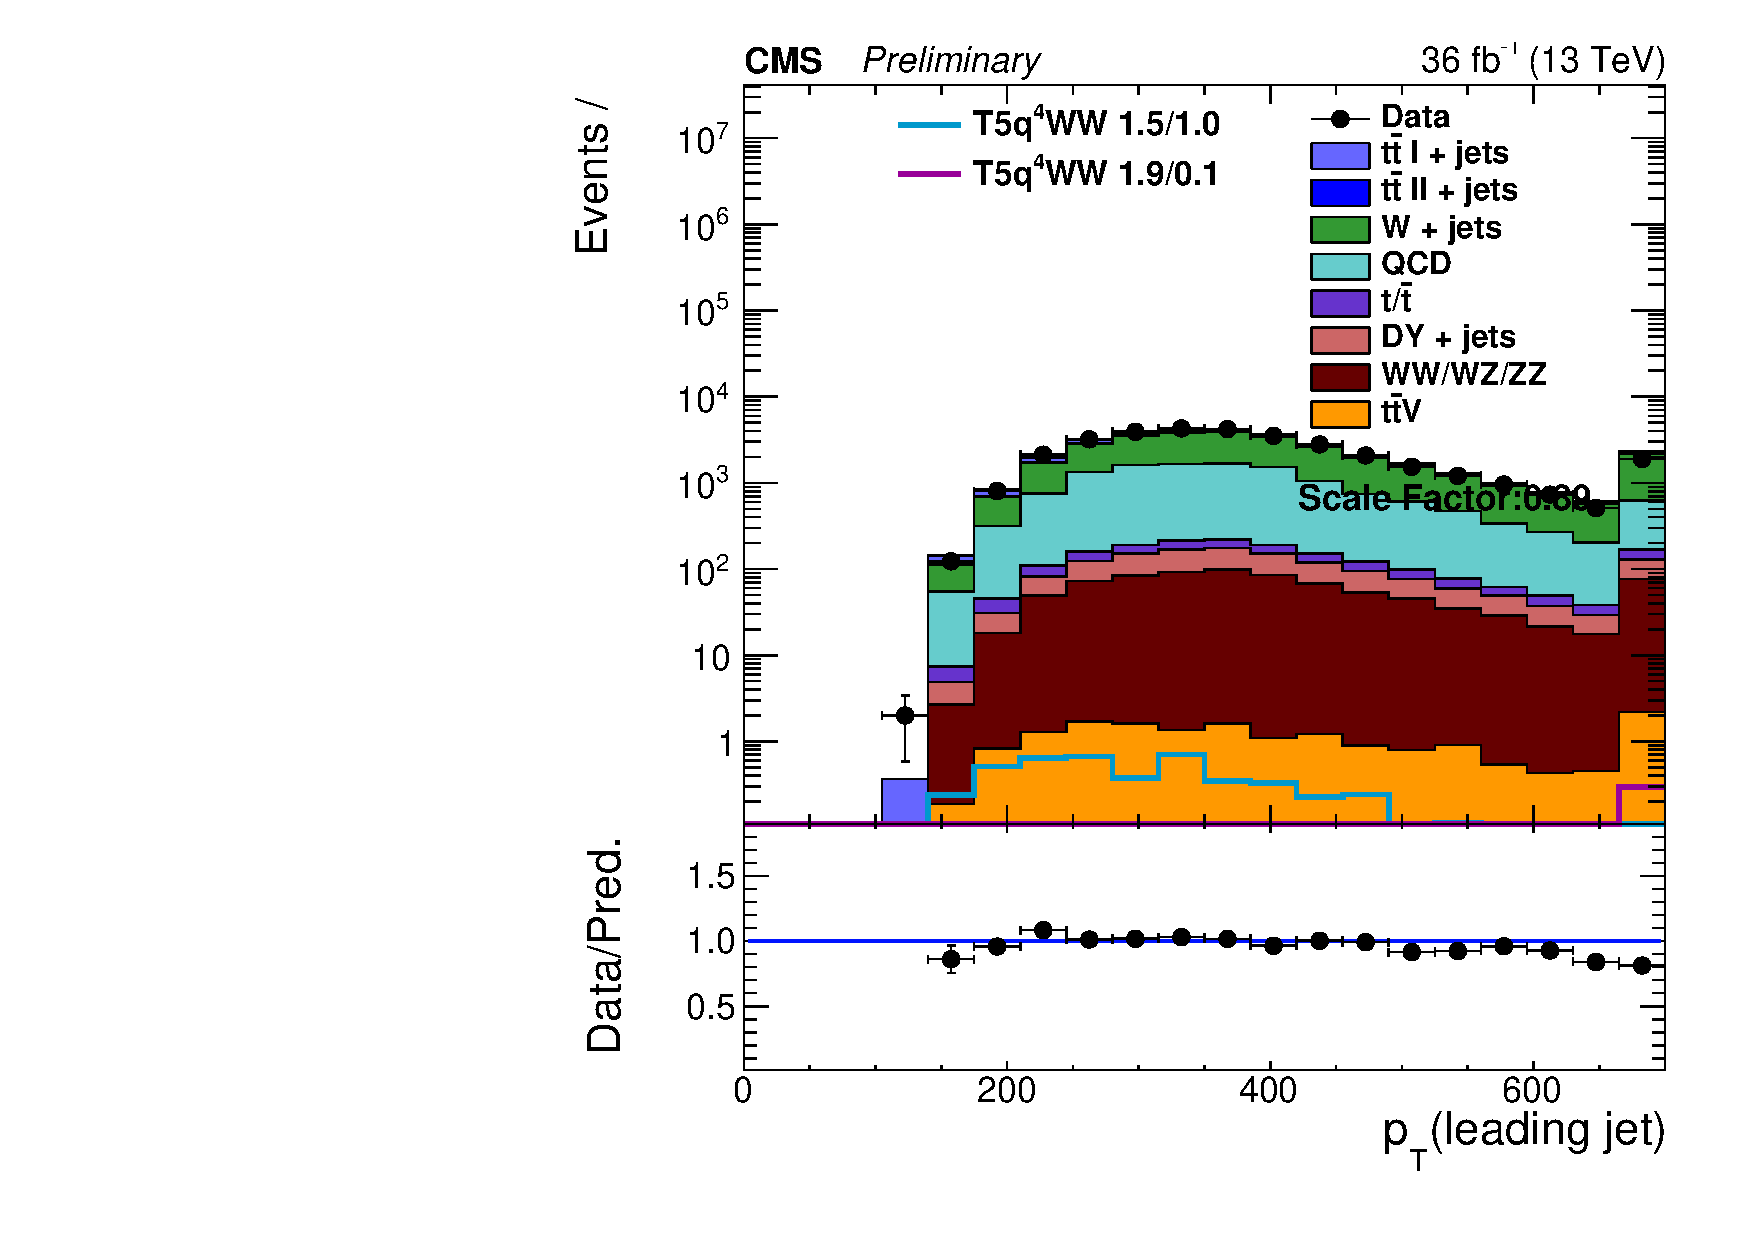
\includegraphics[angle=0,width=.32\textwidth]{Plots//analysis/control_Plots/ele/st250_ht500_njet3-4_nbtagEq0/leading_JetPt.pdf}}
    \subfigure[$n_{\textrm{vertex}}$]{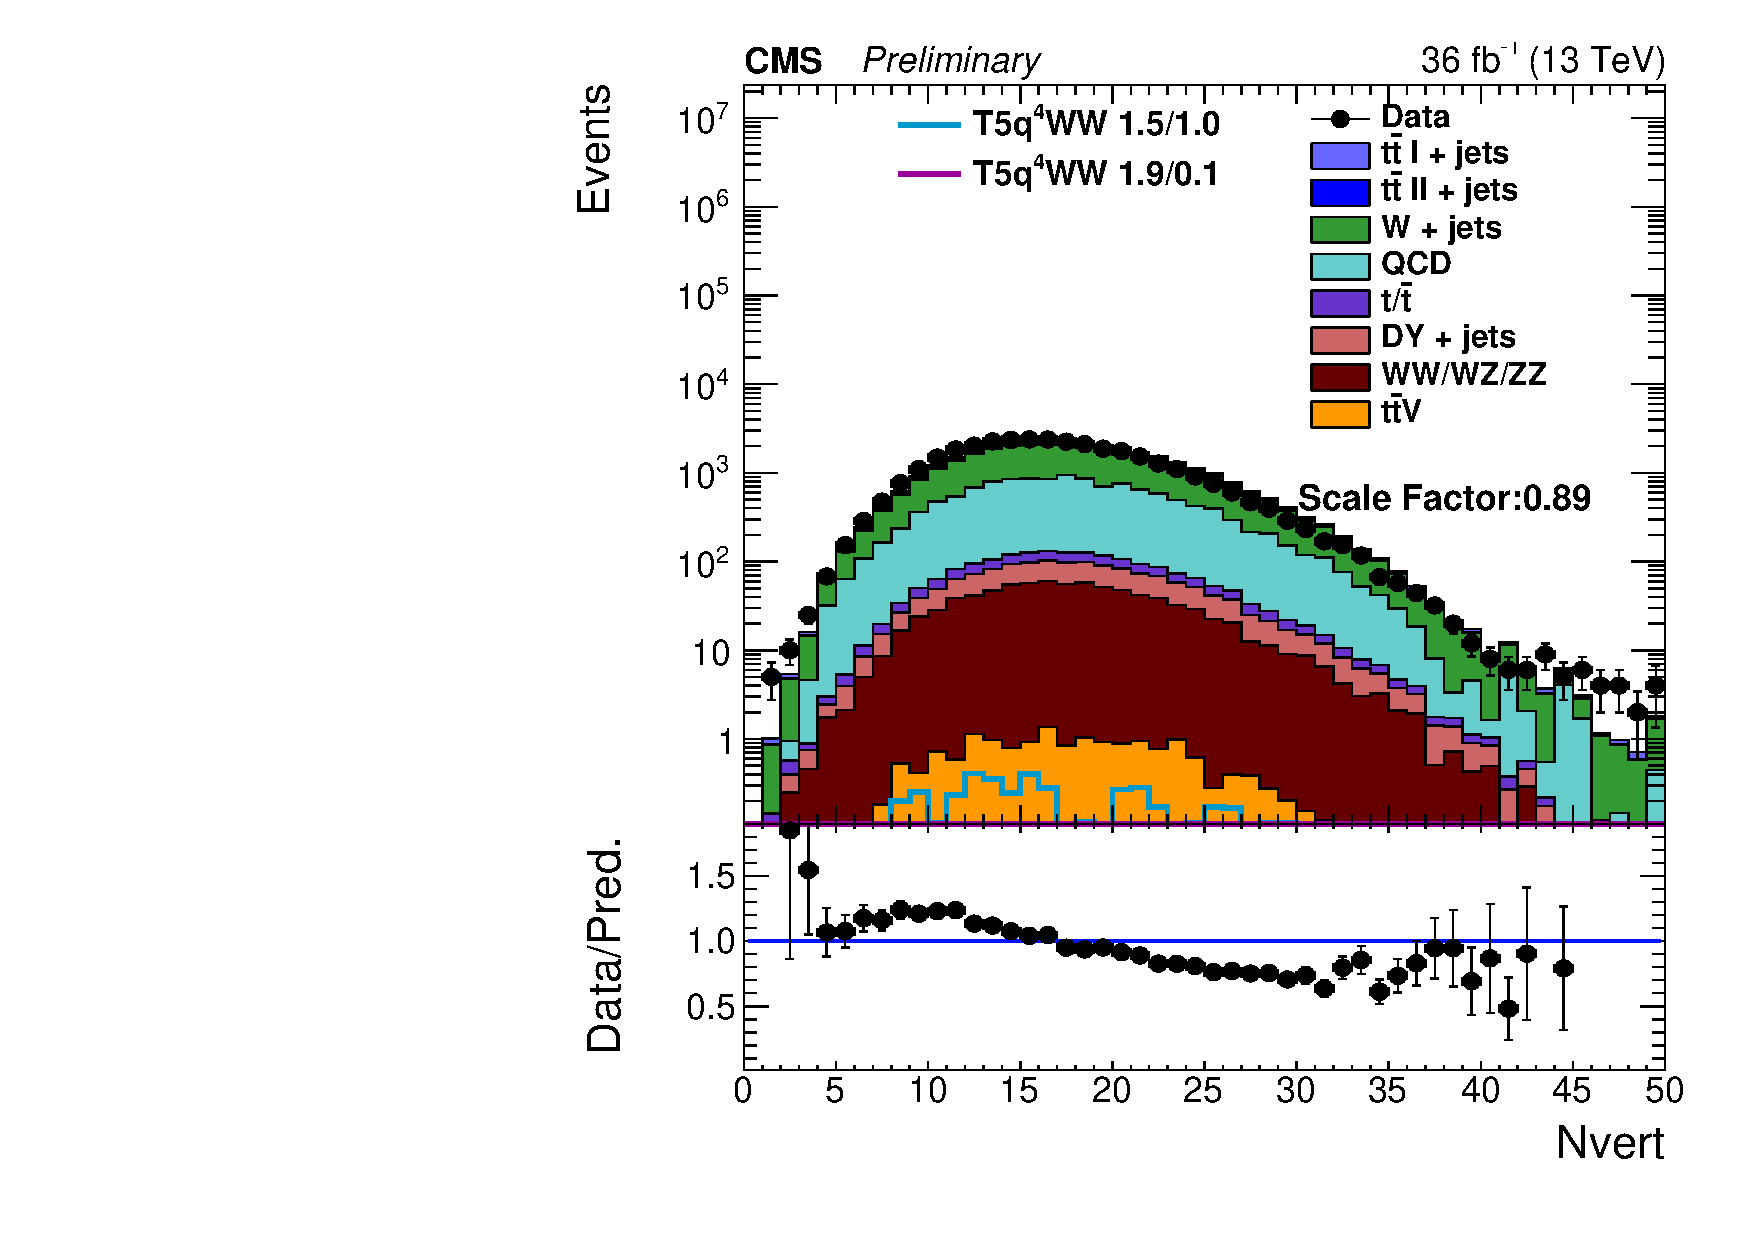
\includegraphics[angle=0,width=.32\textwidth]       {Plots//analysis/control_Plots/ele/st250_ht500_njet3-4_nbtagEq0/nVert.pdf}}\\
    \subfigure[$p_T(l)$]{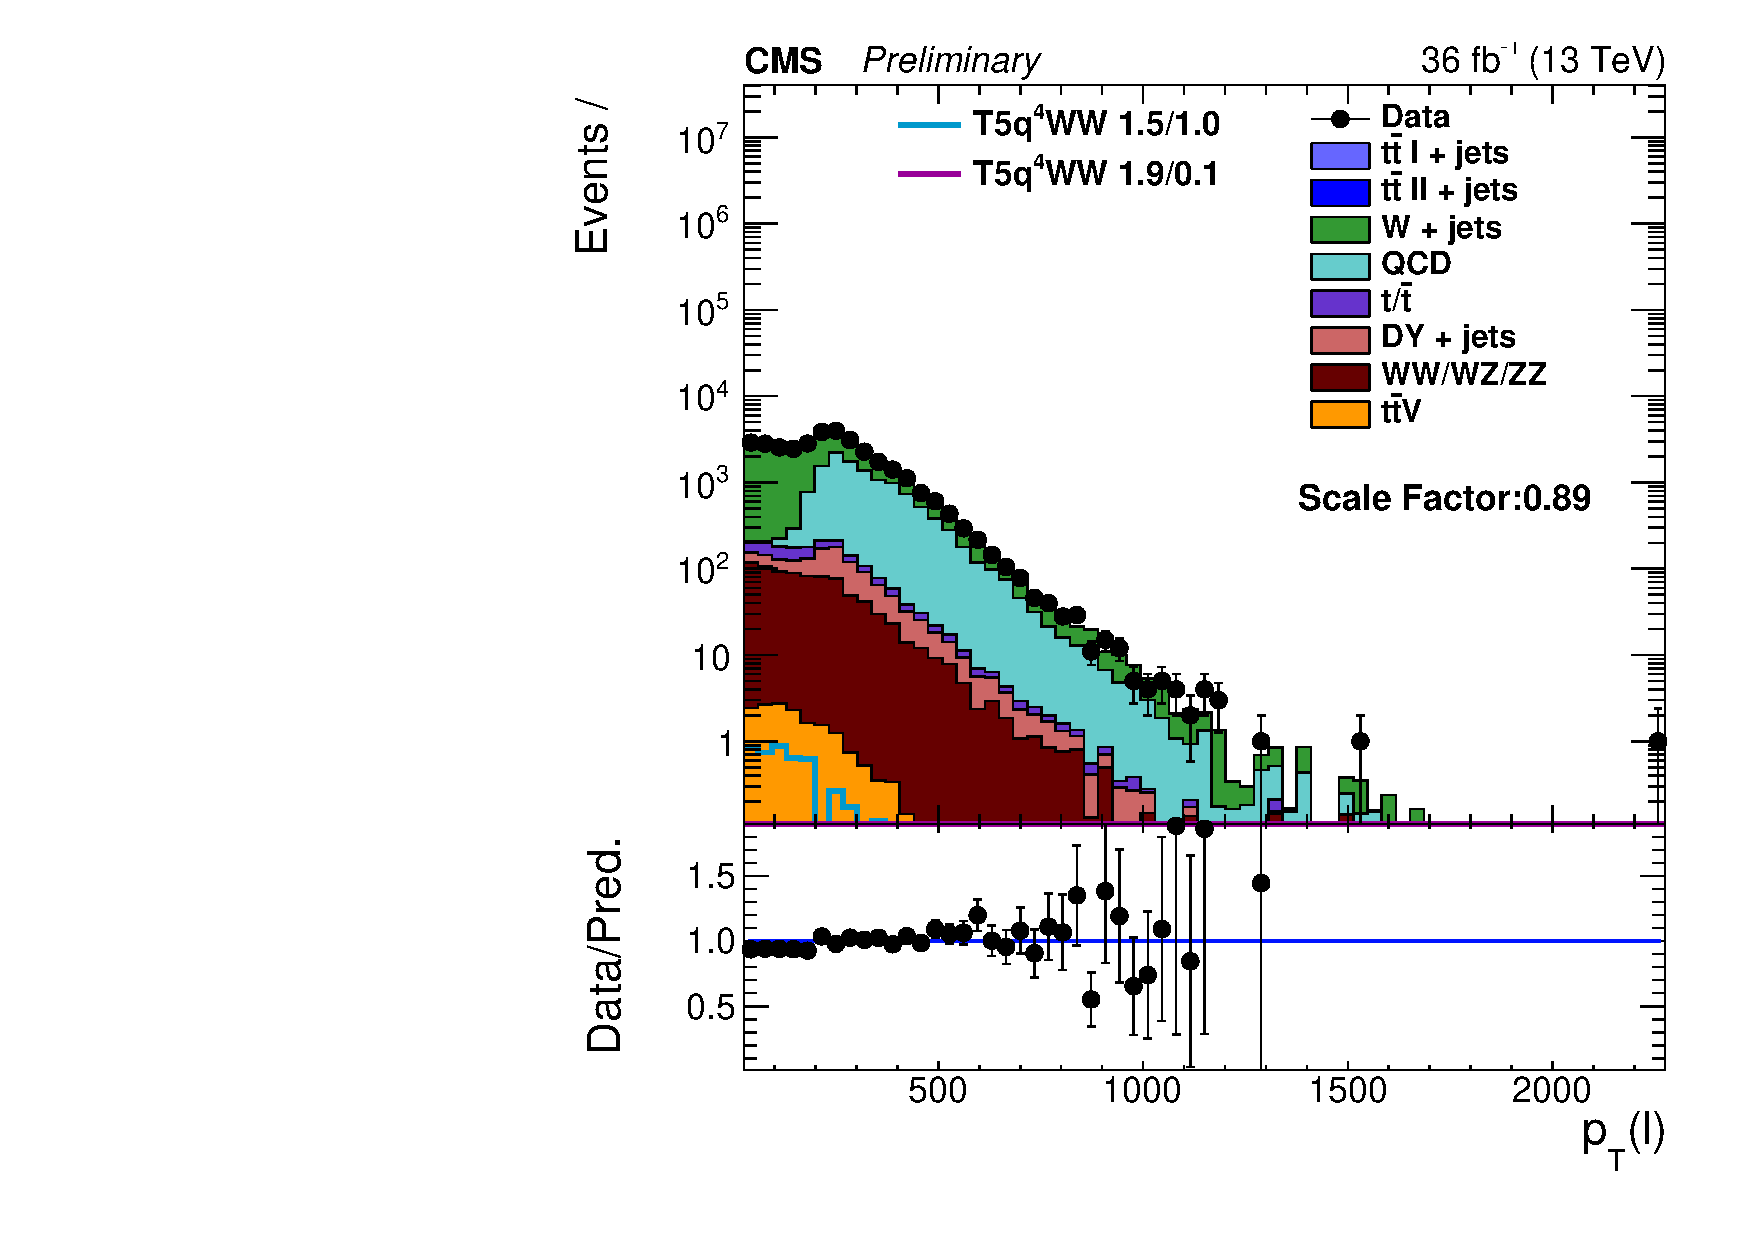
\includegraphics[angle=0,width=.32\textwidth]               {Plots//analysis/control_Plots/ele/st250_ht500_njet3-4_nbtagEq0/leptonPt.pdf}}
    \subfigure[$m_{T2}$]{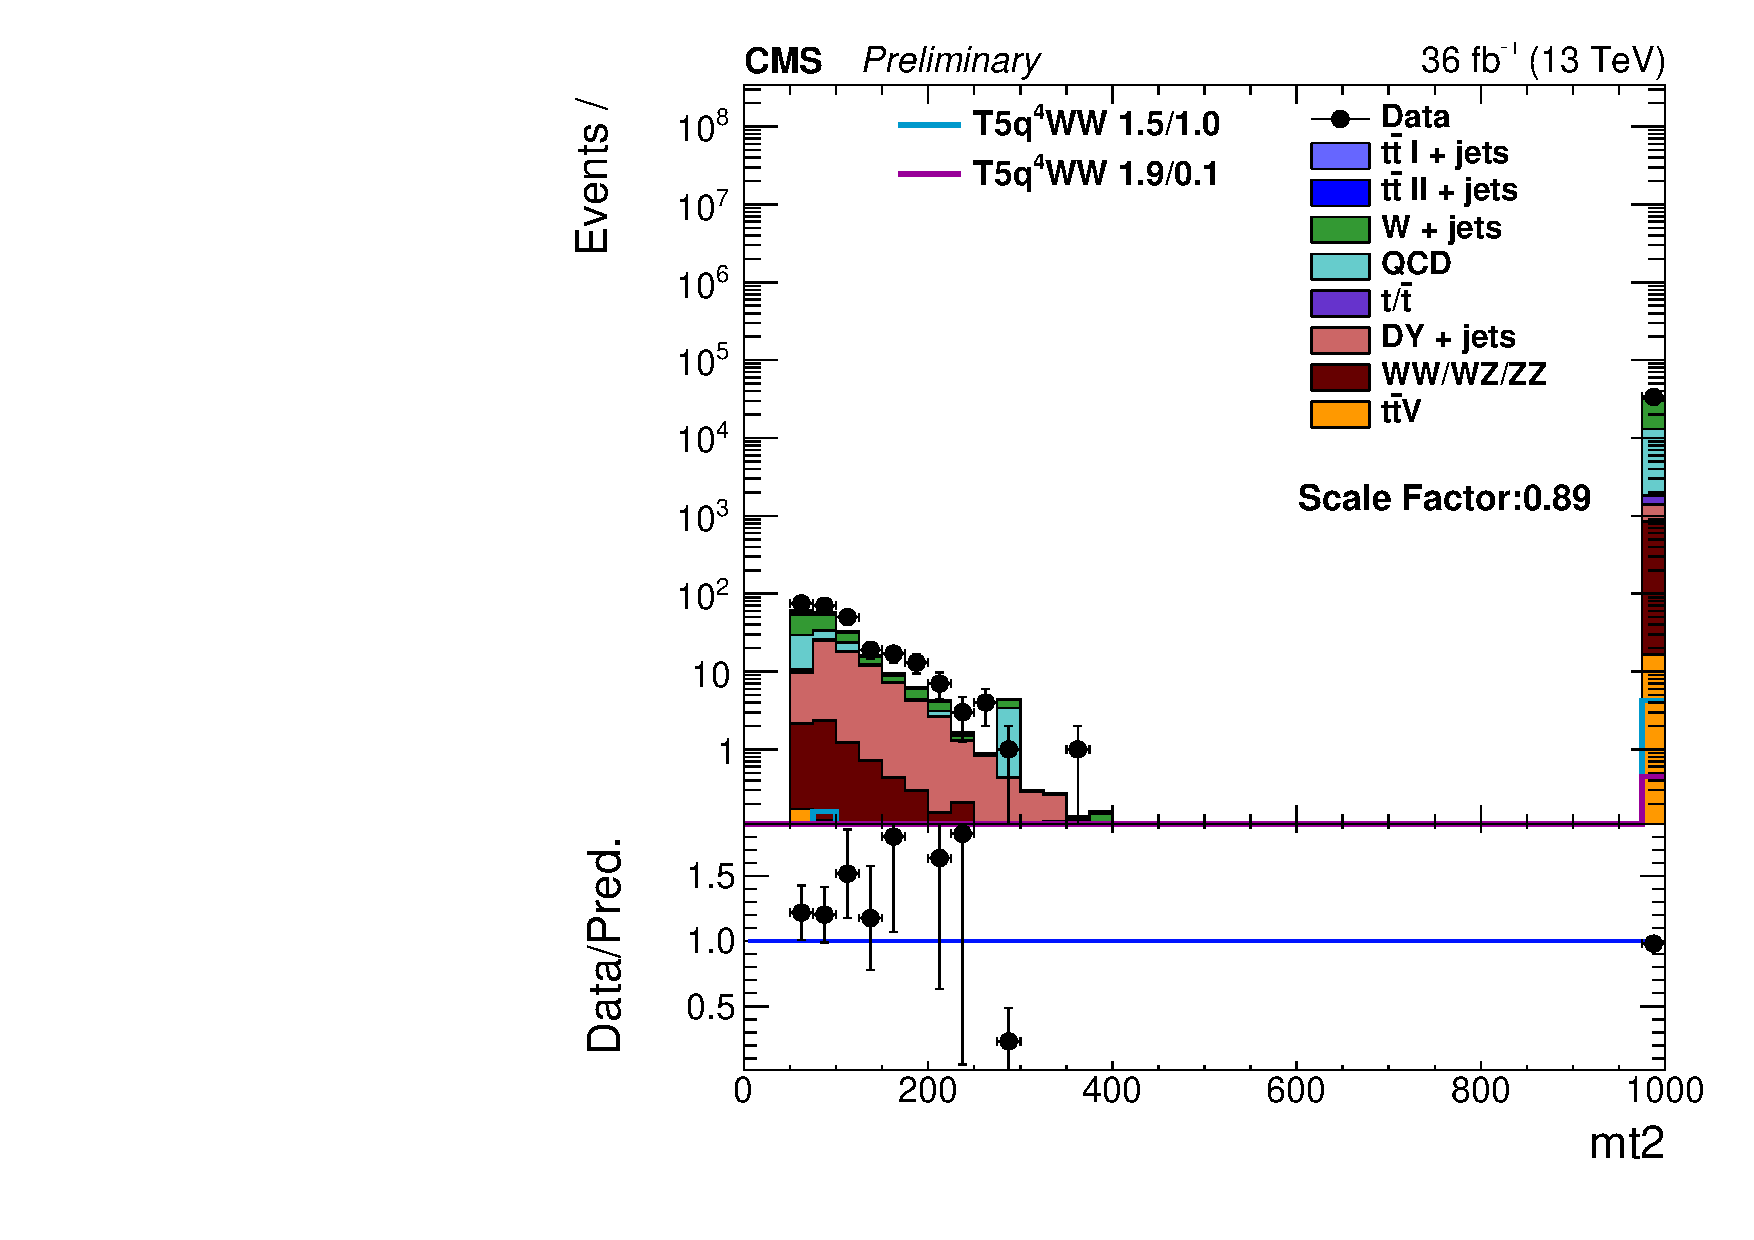
\includegraphics[angle=0,width=.32\textwidth]              {Plots//analysis/control_Plots/ele/st250_ht500_njet3-4_nbtagEq0/iso_MT2.pdf}}
    \subfigure[miniIsolation$(l)$]{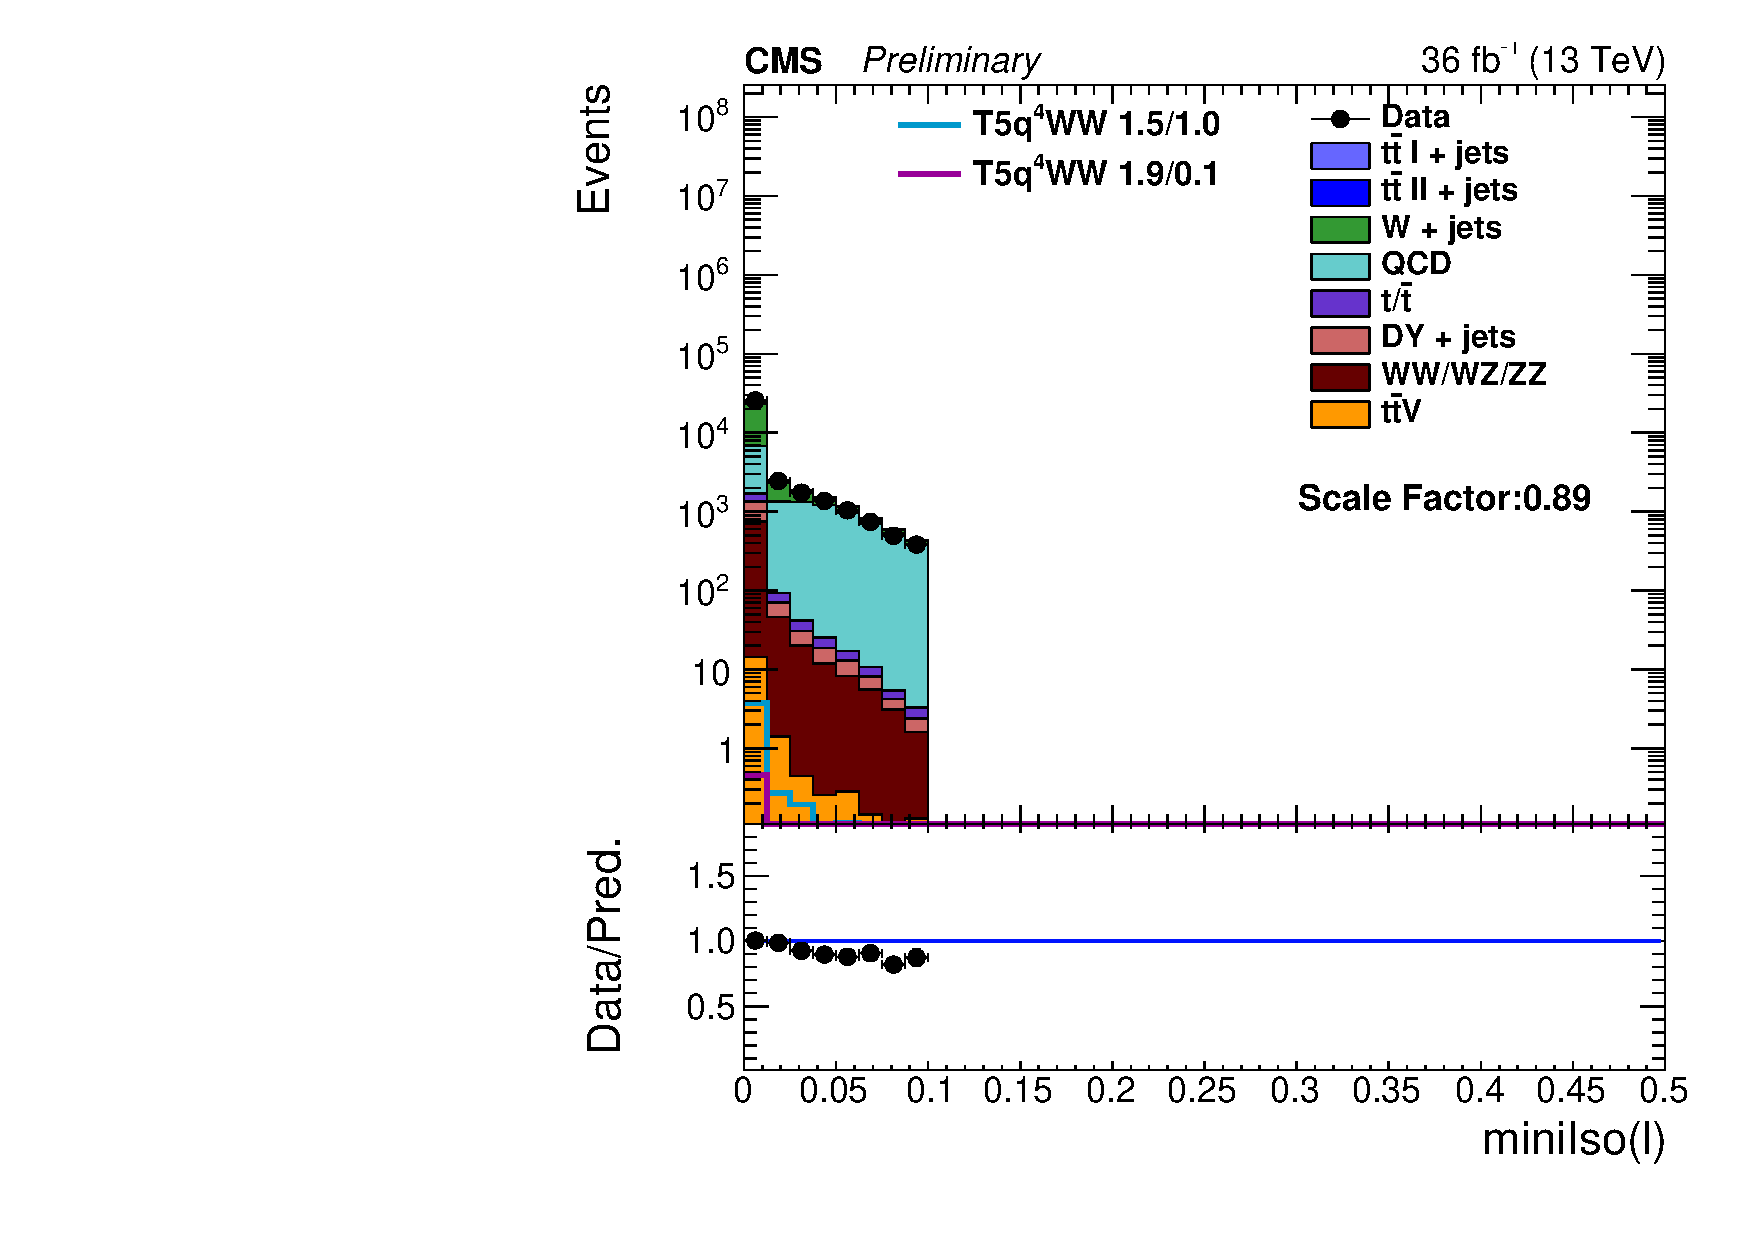
\includegraphics[angle=0,width=.32\textwidth]     {Plots//analysis/control_Plots/ele/st250_ht500_njet3-4_nbtagEq0/leptonminiIso.pdf}}\\
    \subfigure[\HT]{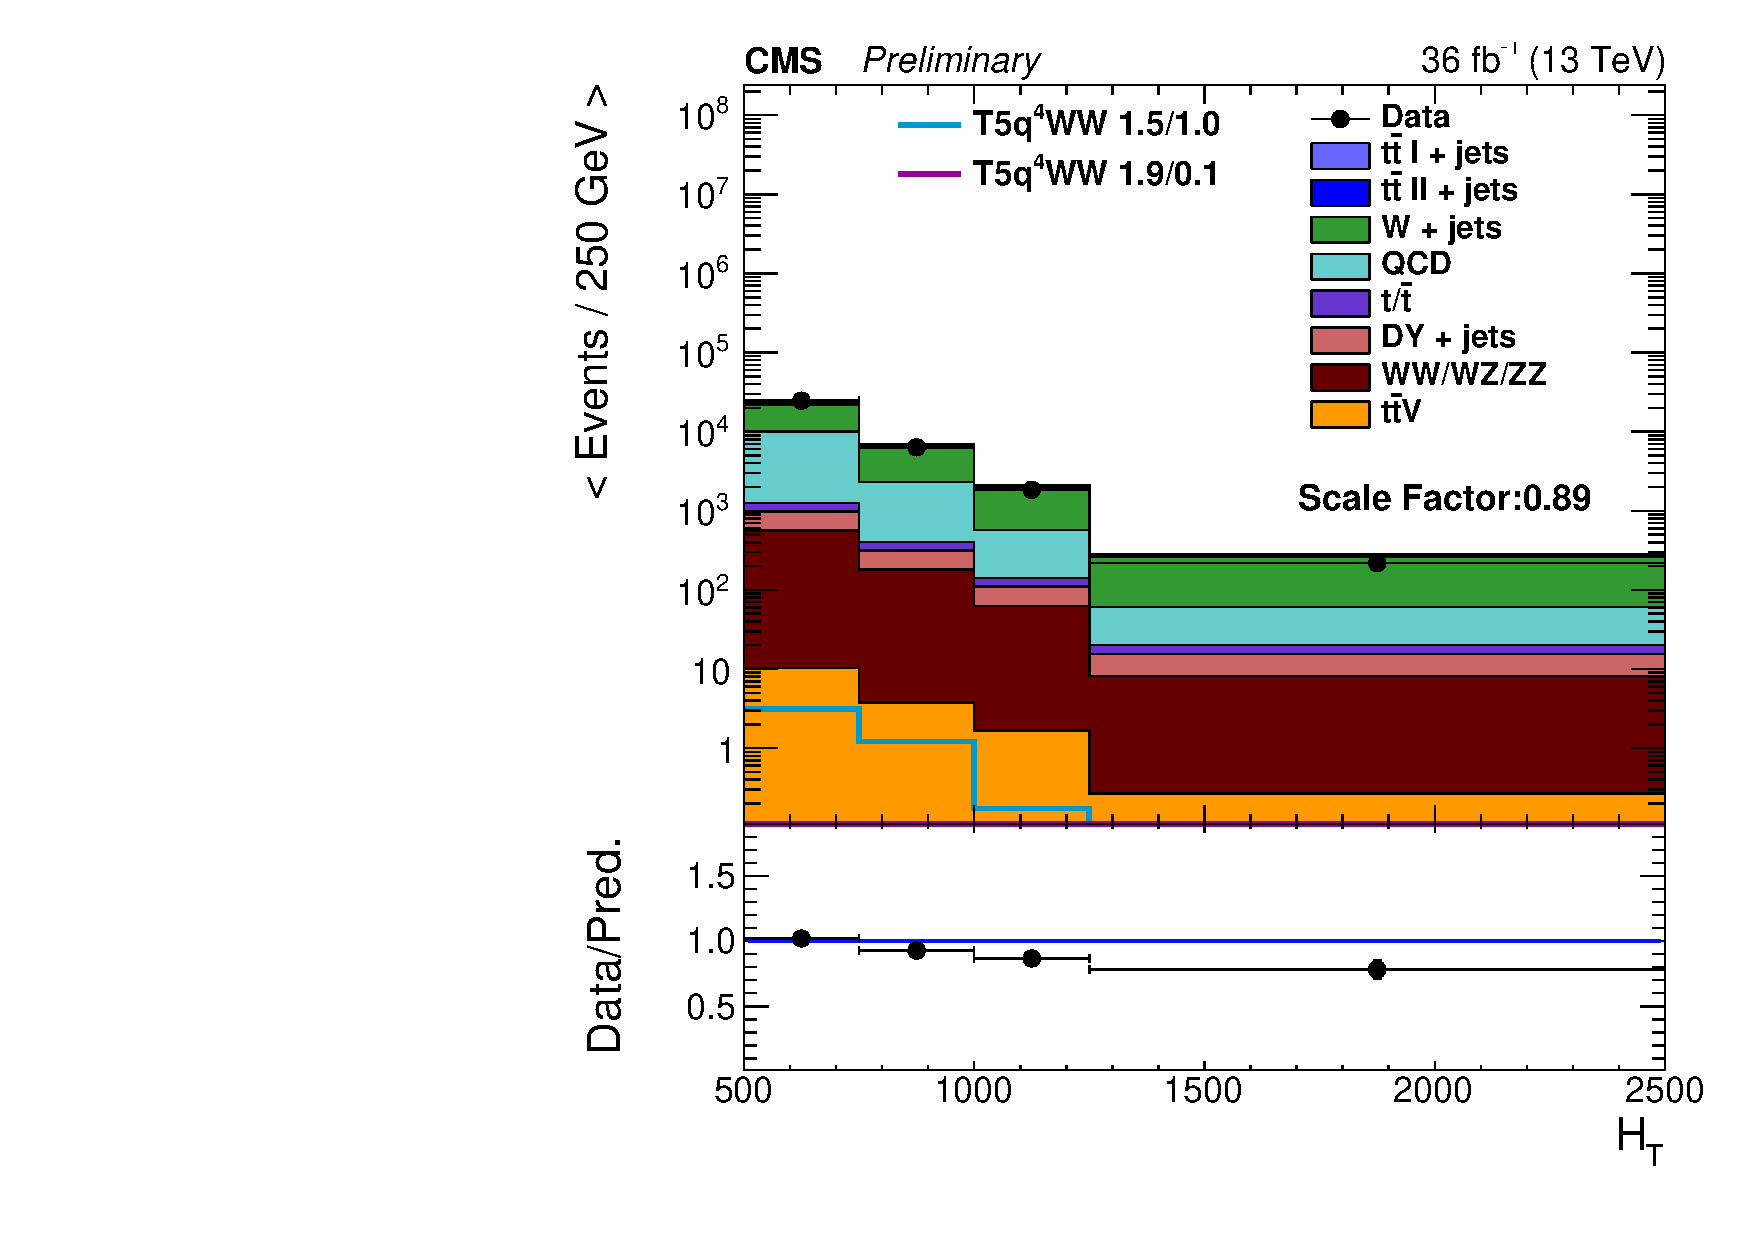
\includegraphics[angle=0,width=.32\textwidth]                    {Plots//analysis/control_Plots/ele/st250_ht500_njet3-4_nbtagEq0/htJet30j.pdf}}
    \subfigure[\LT]{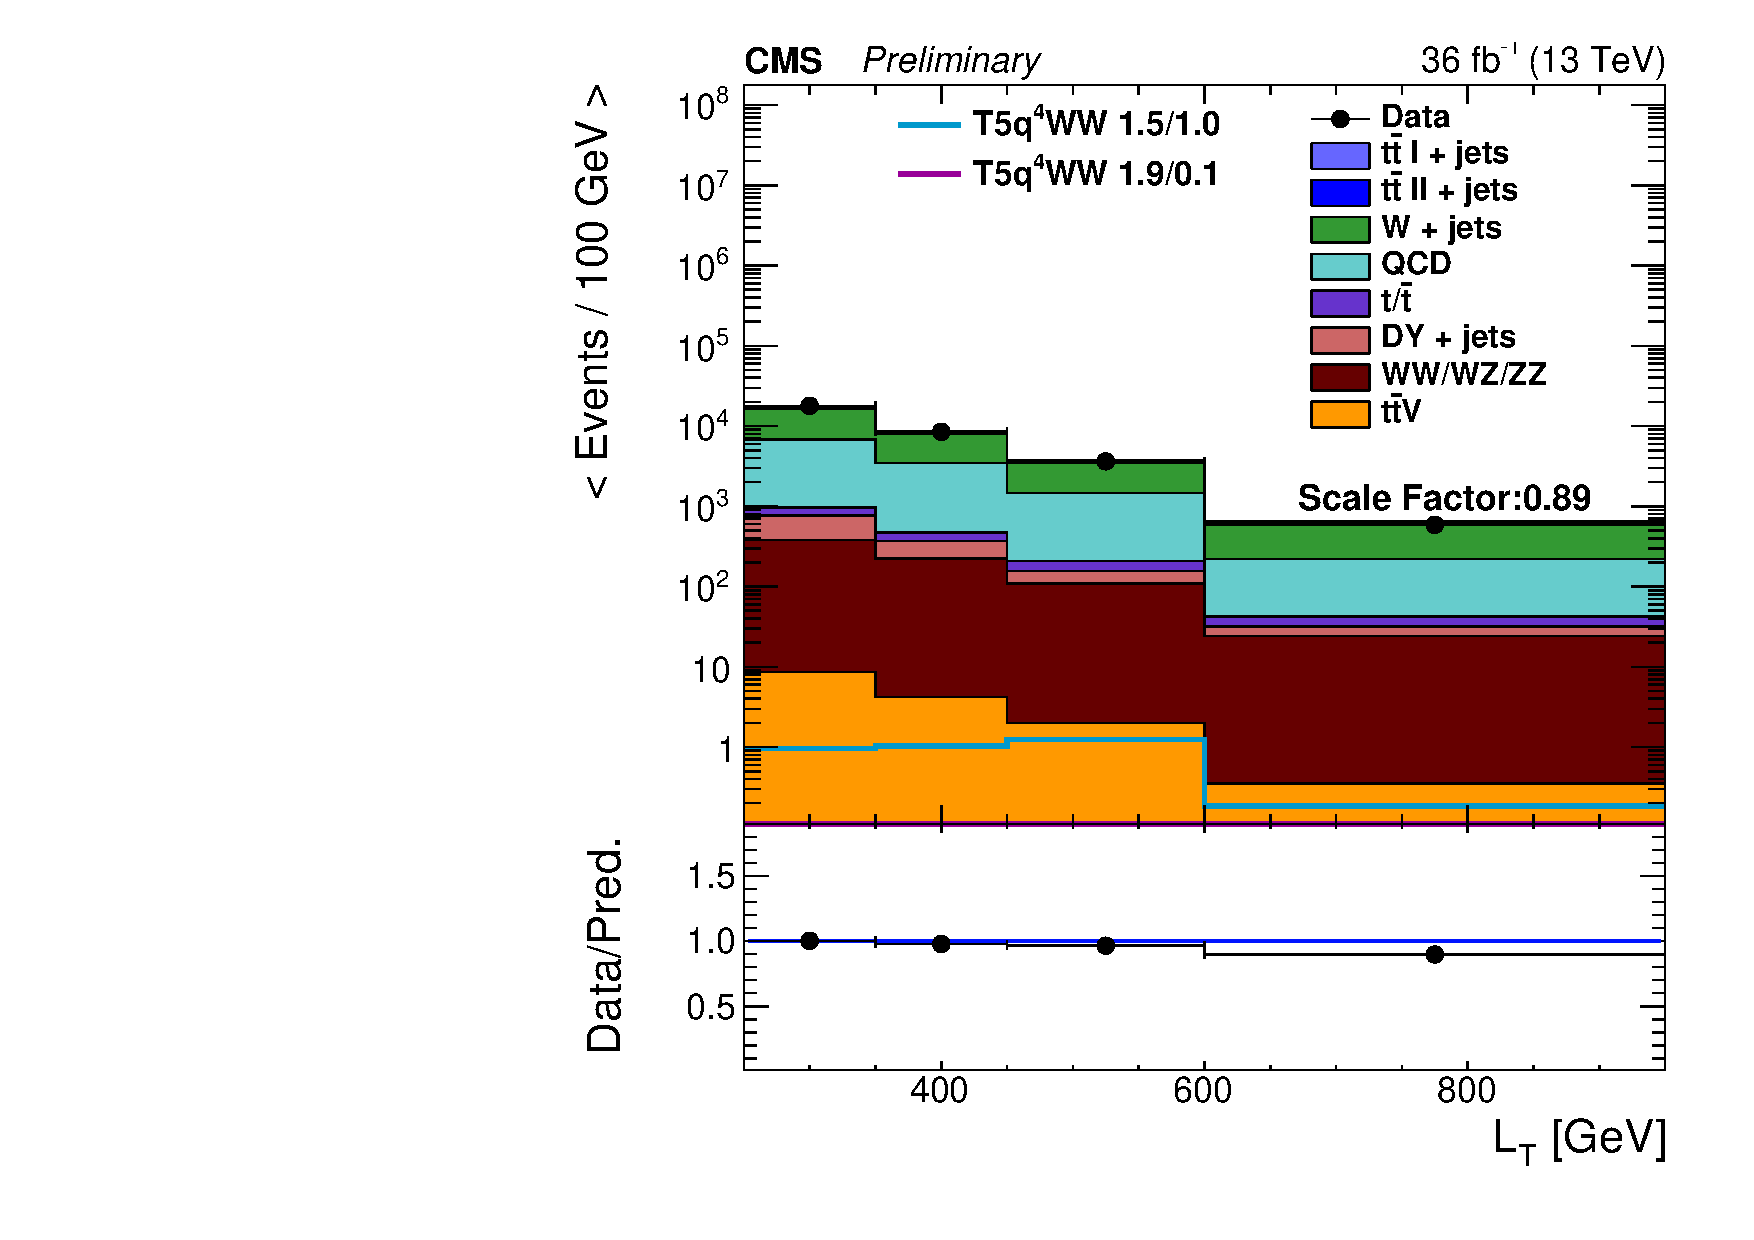
\includegraphics[angle=0,width=.32\textwidth]                    {Plots//analysis/control_Plots/ele/st250_ht500_njet3-4_nbtagEq0/LT.pdf}}
    \subfigure[\DF]{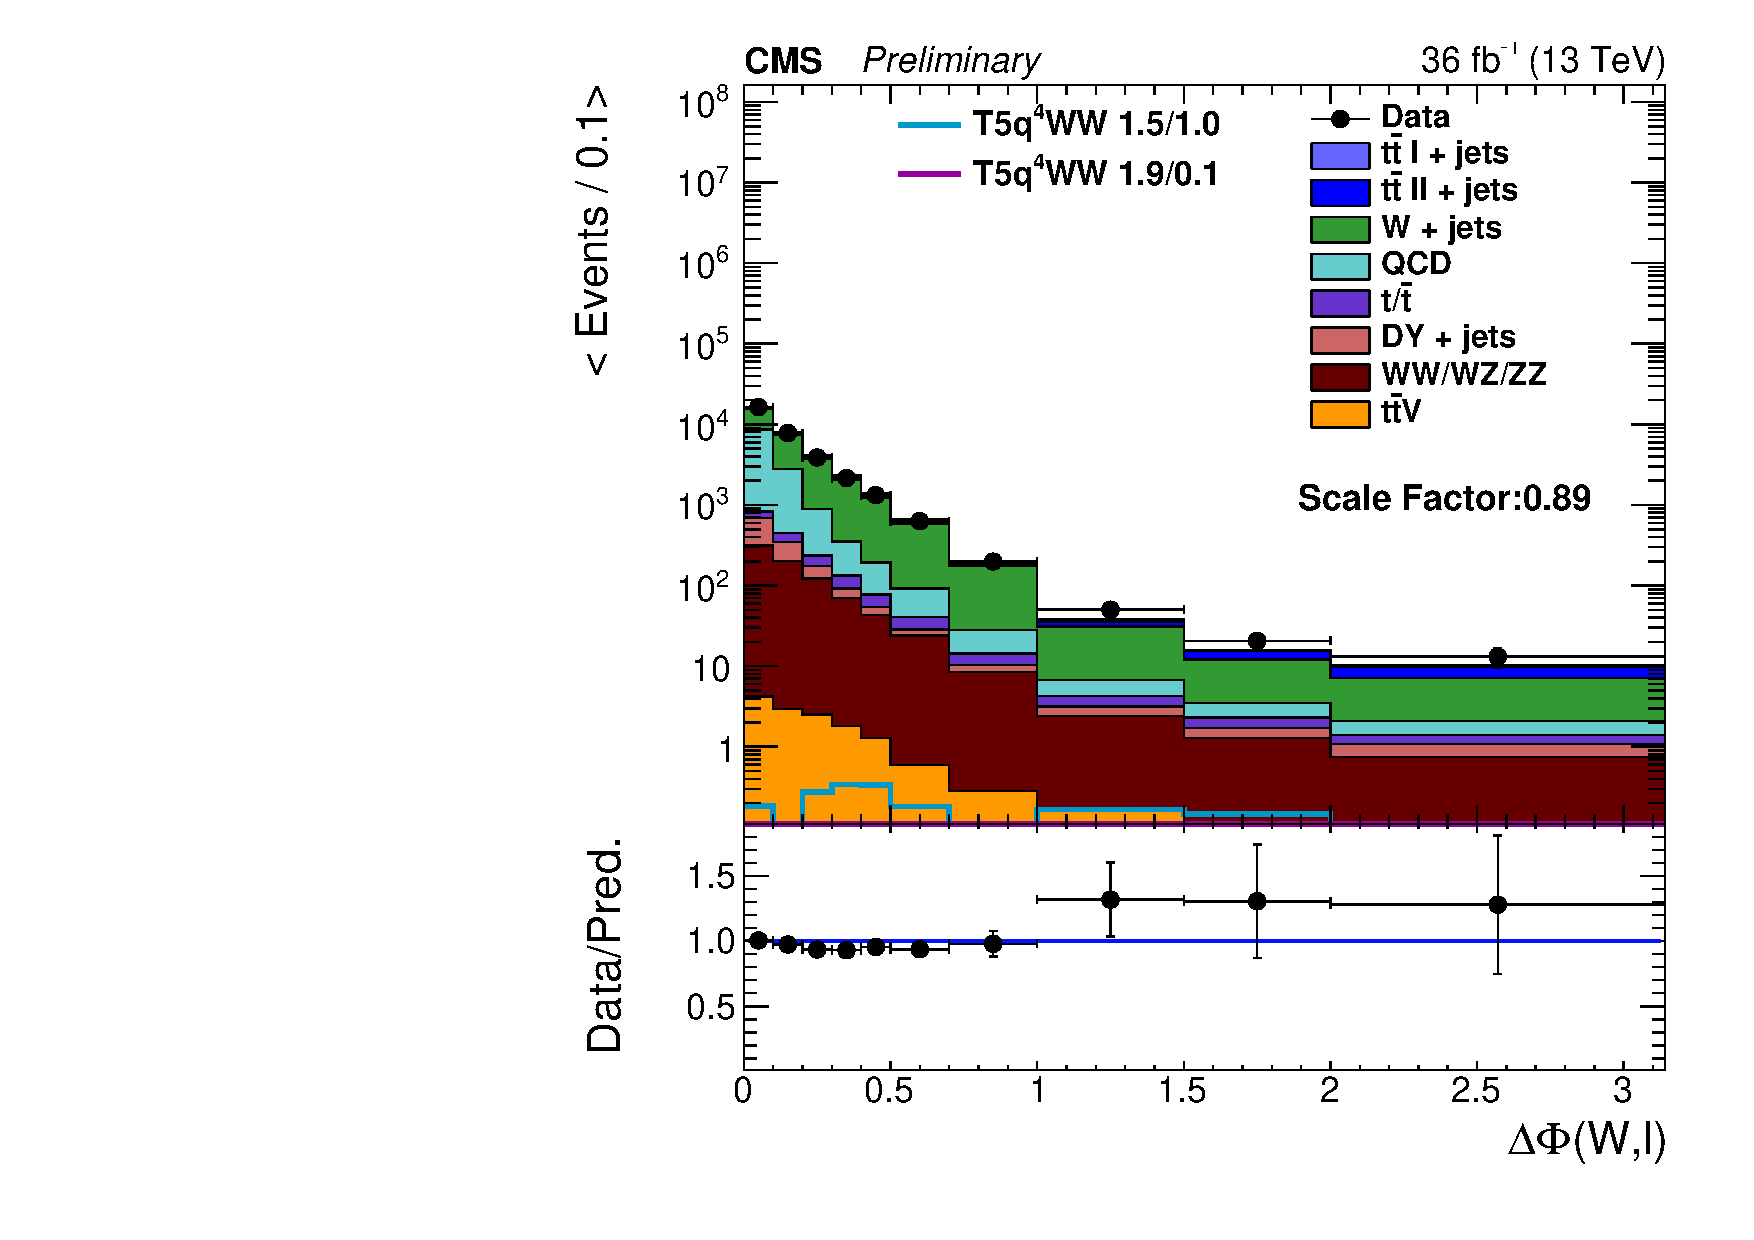
\includegraphics[angle=0,width=.32\textwidth]                    {Plots//analysis/control_Plots/ele/st250_ht500_njet3-4_nbtagEq0/deltaPhi_Wl.pdf}}

    \caption{Distribution of kinematic observables after requiring $\HT >$ 500 \GeV, $\LT >$ 250 \GeV, $3\leq$ jets $\leq4$  and zero b-tagged jets (1 $e$ channel).
      %In order to blind the signal region, data events with large \DF (corresponding to the dynamic \DF cut) are excluded from the \DF plot.
    }
    \label{fig:0bele_zeroB_3_4jets_CR}
  \end{center}
\end{figure}


\begin{figure}[p]
  \begin{center}
    \subfigure[\njet]{\includegraphics[angle=0,width=.32\textwidth]                  {Plots//analysis/control_Plots/mu/st250_ht500_njet4-5_nbtag1/nJet30.pdf}}
    \subfigure[$p_T(\textrm{1st jet})$]{\includegraphics[angle=0,width=.32\textwidth]{Plots//analysis/control_Plots/mu/st250_ht500_njet4-5_nbtag1/leading_JetPt.pdf}}
    \subfigure[$n_{\textrm{vertex}}$]{\includegraphics[angle=0,width=.32\textwidth]       {Plots//analysis/control_Plots/mu/st250_ht500_njet4-5_nbtag1/nVert.pdf}}\\
    \subfigure[$p_T(l)$]{\includegraphics[angle=0,width=.32\textwidth]               {Plots//analysis/control_Plots/mu/st250_ht500_njet4-5_nbtag1/leptonPt.pdf}}
    \subfigure[$m_{T2}$]{\includegraphics[angle=0,width=.32\textwidth]              {Plots//analysis/control_Plots/mu/st250_ht500_njet4-5_nbtag1/iso_MT2.pdf}}
    \subfigure[miniIsolation$(l)$]{\includegraphics[angle=0,width=.32\textwidth]     {Plots//analysis/control_Plots/mu/st250_ht500_njet4-5_nbtag1/leptonminiIso.pdf}}\\
    \subfigure[\HT]{\includegraphics[angle=0,width=.32\textwidth]                    {Plots//analysis/control_Plots/mu/st250_ht500_njet4-5_nbtag1/htJet30j.pdf}}
    \subfigure[\LT]{\includegraphics[angle=0,width=.32\textwidth]                    {Plots//analysis/control_Plots/mu/st250_ht500_njet4-5_nbtag1/LT.pdf}}
    \subfigure[\DF]{\includegraphics[angle=0,width=.32\textwidth]                    {Plots//analysis/control_Plots/mu/st250_ht500_njet4-5_nbtag1/deltaPhi_Wl.pdf}}

    \caption{Distribution of kinematic observables after requiring $\HT >$ 500 \GeV, $\LT >$ 250 \GeV, $4\leq$ jets $\leq5$  and  b-tagged jets (1 $\mu$ channel).
      %In order to blind the signal region, data events with large \DF (corresponding to the dynamic \DF cut) are excluded from the \DF plot.
    }
    \label{fig:0bmu_1B_4_5jets_CR}
  \end{center}
\end{figure}

\begin{figure}[p]
  \begin{center}
    \subfigure[\njet]{\includegraphics[angle=0,width=.32\textwidth]                  {Plots//analysis/control_Plots/ele/st250_ht500_njet4-5_nbtag1/nJet30.pdf}}
    \subfigure[$p_T(\textrm{1st jet})$]{\includegraphics[angle=0,width=.32\textwidth]{Plots//analysis/control_Plots/ele/st250_ht500_njet4-5_nbtag1/leading_JetPt.pdf}}
    \subfigure[$n_{\textrm{vertex}}$]{\includegraphics[angle=0,width=.32\textwidth]       {Plots//analysis/control_Plots/ele/st250_ht500_njet4-5_nbtag1/nVert.pdf}}\\
    \subfigure[$p_T(l)$]{\includegraphics[angle=0,width=.32\textwidth]               {Plots//analysis/control_Plots/ele/st250_ht500_njet4-5_nbtag1/leptonPt.pdf}}
    \subfigure[$m_{T2}$]{\includegraphics[angle=0,width=.32\textwidth]              {Plots//analysis/control_Plots/ele/st250_ht500_njet4-5_nbtag1/iso_MT2.pdf}}
    \subfigure[miniIsolation$(l)$]{\includegraphics[angle=0,width=.32\textwidth]     {Plots//analysis/control_Plots/ele/st250_ht500_njet4-5_nbtag1/leptonminiIso.pdf}}\\
    \subfigure[\HT]{\includegraphics[angle=0,width=.32\textwidth]                    {Plots//analysis/control_Plots/ele/st250_ht500_njet4-5_nbtag1/htJet30j.pdf}}
    \subfigure[\LT]{\includegraphics[angle=0,width=.32\textwidth]                    {Plots//analysis/control_Plots/ele/st250_ht500_njet4-5_nbtag1/LT.pdf}}
    \subfigure[\DF]{\includegraphics[angle=0,width=.32\textwidth]                    {Plots//analysis/control_Plots/ele/st250_ht500_njet4-5_nbtag1/deltaPhi_Wl.pdf}}

    \caption{Distribution of kinematic observables after requiring $\HT >$ 500 \GeV, $\LT >$ 250 \GeV, $4\leq$ jets $\leq5$  and b-tagged jets (1 $e$ channel).
      %In order to blind the signal region, data events with large \DF (corresponding to the dynamic \DF cut) are excluded from the \DF plot.
    }
    \label{fig:0bele_1B_4_5jets_CR}
  \end{center}
\end{figure}


\begin{figure}[p]
  \begin{center}
    \subfigure[\njet]{\includegraphics[angle=0,width=.32\textwidth]                  {Plots//analysis/control_Plots/mu/st250_ht500_njet5_nbtagEq0/nJet30.pdf}}
    \subfigure[$p_T(\textrm{1st jet})$]{\includegraphics[angle=0,width=.32\textwidth]{Plots//analysis/control_Plots/mu/st250_ht500_njet5_nbtagEq0/leading_JetPt.pdf}}
    \subfigure[$n_{\textrm{vertex}}$]{\includegraphics[angle=0,width=.32\textwidth]       {Plots//analysis/control_Plots/mu/st250_ht500_njet5_nbtagEq0/nVert.pdf}}\\
    \subfigure[$p_T(l)$]{\includegraphics[angle=0,width=.32\textwidth]               {Plots//analysis/control_Plots/mu/st250_ht500_njet5_nbtagEq0/leptonPt.pdf}}
    \subfigure[$m_{T2}$]{\includegraphics[angle=0,width=.32\textwidth]              {Plots//analysis/control_Plots/mu/st250_ht500_njet5_nbtagEq0/iso_MT2.pdf}}
    \subfigure[miniIsolation$(l)$]{\includegraphics[angle=0,width=.32\textwidth]     {Plots//analysis/control_Plots/mu/st250_ht500_njet5_nbtagEq0/leptonminiIso.pdf}}\\
    \subfigure[\HT]{\includegraphics[angle=0,width=.32\textwidth]                    {Plots//analysis/control_Plots/mu/st250_ht500_njet5_nbtagEq0/htJet30j.pdf}}
    \subfigure[\LT]{\includegraphics[angle=0,width=.32\textwidth]                    {Plots//analysis/control_Plots/mu/st250_ht500_njet5_nbtagEq0/LT.pdf}}
    \subfigure[\DF]{\includegraphics[angle=0,width=.32\textwidth]                    {Plots//analysis/control_Plots/mu/st250_ht500_njet5_nbtagEq0/deltaPhi_Wl.pdf}}
    \caption{Distribution of kinematic observables after requiring $\HT >$ 500 \GeV, $\LT >$ 250 \GeV, $\geq$ 5 jets and zero b-tagged jets (1 $\mu$ channel).
    }
    \label{fig:0bmu_0p5_CR}
  \end{center}
\end{figure}


\begin{figure}[p]
  \begin{center}
    \subfigure[\njet]{\includegraphics[angle=0,width=.32\textwidth]                  {Plots//analysis/control_Plots/ele/st250_ht500_njet5_nbtagEq0/nJet30.pdf}}
    \subfigure[$p_T(\textrm{1st jet})$]{\includegraphics[angle=0,width=.32\textwidth]{Plots//analysis/control_Plots/ele/st250_ht500_njet5_nbtagEq0/leading_JetPt.pdf}}
    \subfigure[$n_{\textrm{vertex}}$]{\includegraphics[angle=0,width=.32\textwidth]       {Plots//analysis/control_Plots/ele/st250_ht500_njet5_nbtagEq0/nVert.pdf}}\\
    \subfigure[$p_T(l)$]{\includegraphics[angle=0,width=.32\textwidth]               {Plots//analysis/control_Plots/ele/st250_ht500_njet5_nbtagEq0/leptonPt.pdf}}
    \subfigure[$m_{T2}$]{\includegraphics[angle=0,width=.32\textwidth]              {Plots//analysis/control_Plots/ele/st250_ht500_njet5_nbtagEq0/iso_MT2.pdf}}
    \subfigure[miniIsolation$(l)$]{\includegraphics[angle=0,width=.32\textwidth]     {Plots//analysis/control_Plots/ele/st250_ht500_njet5_nbtagEq0/leptonminiIso.pdf}}\\
    \subfigure[\HT]{\includegraphics[angle=0,width=.32\textwidth]                    {Plots//analysis/control_Plots/ele/st250_ht500_njet5_nbtagEq0/htJet30j.pdf}}
    \subfigure[\LT]{\includegraphics[angle=0,width=.32\textwidth]                    {Plots//analysis/control_Plots/ele/st250_ht500_njet5_nbtagEq0/LT.pdf}}
    \subfigure[\DF]{\includegraphics[angle=0,width=.32\textwidth]                    {Plots//analysis/control_Plots/ele/st250_ht500_njet5_nbtagEq0/deltaPhi_Wl.pdf}}

    \caption{Distribution of kinematic observables after requiring $\HT >$ 500 \GeV, $\LT >$ 250 \GeV, $\geq$ 5 jets and zero b-tagged jets (1 $e$ channel).
    }
    \label{fig:0bele_0p5_CR}
  \end{center}
\end{figure}

\chapter{Statistical Tests}
\label{sec:nuisances}
In this appendix, the output of the maximum likelihood fit to the data, in particular the effect of the different nuisance parameters is investigated.
The tests are performed with the datacard of the mass point T5qqqqqWW 1900/100.
\begin{figure}[!hbtp]
\begin{center}
\subfigure[lnN constraints on region A]{\includegraphics[width=0.5\textwidth]{Plots/nuisances/nuisances-other.pdf}}\\
\subfigure[$\kappa$ parameters]{\includegraphics[width=0.5\textwidth]{Plots/nuisances/nuisances-kJ.pdf}} \\
\subfigure[QCD estimate]{\includegraphics[width=0.5\textwidth]{Plots/nuisances/nuisances-QCD.pdf}}\\
\end{center}
\caption{Prefit (grey), s+b postfit (red) and, b-only postfit (blue) values of nuisance parameters included in the fit. }
\label{fig:nuisances1}
\end{figure}

\begin{figure}[!hbtp]
\begin{center}
\subfigure[nuisances in $W$ Side Band]{\includegraphics[width=0.5\textwidth]{Plots/nuisances/nuisances-j3.pdf}} \\
\subfigure[nuisances in $\ttbar$ Side Band]{\includegraphics[width=0.5\textwidth]{Plots/nuisances/nuisances-j4.pdf}} \\
\end{center}
\caption{Prefit (grey), s+b postfit (red) and, b-only postfit (blue) values of nuisance parameters in side band regions included in the fit. }
\label{fig:nuisances2}
\end{figure}
\listoffigures              % generate and include a list of figures
\listoftables
%\begin{glossary}
%\end{glossary}
%\clearpage

%\newglossaryentry{domain-knowledge}{%
%  name={domain knowledge},%
%  description={valid knowledge used to refer to an area of human endeavour, an autonomous computer activity, or other specialized discipline}}

\newacronym{atlas}{ATLAS}{A Toroidal LHC Apparatus}
\newacronym{alice}{ALICE}{A Large Ion Collider Experiment}
\newacronym{sm}{SM}{Standard Model}
\newacronym{susy}{SUSY}{Supersymmetry}
\newacronym{bsm}{BSM}{Beyond the Standard Model}
\newacronym{cern}{CERN}{European Organization for Nuclear Research}
\newacronym{cm}{CM}{Center of Mass}
\newacronym{cms}{CMS}{Compact Muon Solenoid}
\newacronym{cmssw}{CMSSW}{CMS SoftWare framework}
\newacronym{daq}{DAQ}{Data Acquisition}
\newacronym{ecal}{ECAL}{Electromagnetic Calorimeter}
\newacronym{ewk}{EWK}{Electroweak Theory}
\newacronym{ewsb}{EWSB}{Electroweak Symmetry Breaking}
\newacronym{gut}{GUT}{Grand Unified Theory}
\newacronym{hcal}{HCAL}{Hadron Calorimeter}
\newacronym{hf}{HF}{Hadron Calorimeter (Forward)}
\newacronym{lhc}{LHC}{Large Hadron Collider}
\newacronym{lhcb}{LHCb}{the Large Hadron Collider Beauty Experiment}
\newacronym{linac}{LINAC}{Linear particle Accelerator}
\newacronym{pdg}{PDG}{Particle Data Group}
\newacronym{qed}{QED}{\textbf{quantum electrodynamics}}
\newacronym{gut}{GUT}{Grand Unified Theory}
\newacronym{qft}{QFT}{Quantum Field Theory}
\newacronym{qcd}{QCD}{\textbf{quantum chromodynamics}}
\newacronym{sms}{SMS}{Simplified Model Spectra}
\newacronym{vev}{VEV}{vacuum expectation value}
\newacronym{ssb}{SSB}{spontaneous breaking of the SM gauge symmetry}
\newacronym{dm}{DM}{Dark Matter}
\newacronym{cmb}{CMB}{cosmic Microwave Background}
\newacronym{lsp}{LSP}{lightest supersymmetric particle}
\newacronym{mssm}{MSSM}{minimal supersymmetric extension of the standard model}
\newacronym{cmssm}{cMSSM}{constrained MSSM}
\newacronym{pf}{PF}{particle flow}

%\begin{abbreviations}
%\noindent
%\begin{longtable}[l]{lp{10cm}}
%ALICE & A Large Ion Collider Experiment\\
%ATLAS & A Toroidal LHC Apparatus\\                 
%BSM   & Beyond the Standard Model\\
%CERN  & European Organization for Nuclear Research\\
%CM    & Center of Mass\\
%CMS   & Compact Muon Solenoid experiment\\
%CMSSW & CMS SoftWare framework\\
%DAQ   & Data Acquisition\\
%ECAL  & Electromagnetic Calorimeter\\
%EWK   & Electroweak Theory\\
%GUT   & Grand Unified Theory\\
%HCAL  & Hadron Calorimeter\\
%HF    & Hadron Calorimeter (Forward)\\
%LHC   & Large Hadron Collider\\
%LHCb  & the Large Hadron Collider Beauty Experiment\\
%LINAC & Linear particle Accelerator\\
%PDG   & Particle Data Group\\
%QED   & Quantum Electrodynamics\\
%QFT   & Quantum Field Theory\\
%SM    & Standard Model\\
%SMS   & Simplified Model Spectra\\
%SUSY  & Supersymmetry\\
%\end{longtable}

%\end{abbreviations}
%\begin{table}[ht]
%\begin{center}
%\begin{tabular}{cccc}
%\multicolumn{4}{ c }{List of Abbreviations}\\
%AA & blablabala & BB & Bla bla\\
%AA & blablabala & BB & Bla bla\\
%AA & blablabala & BB & Bla bla\\
%AA & blablabala & BB & Bla bla\\
%AA & blablabala & BB & Bla bla\\
%\end{tabular}
%\end{center}
%\end{table}
%
%
%



\begin{thebibliography}{99}\fontsize{12}{16.4} \selectfont

\bibitem{R24} J. Beringer et al. (Particle Data Group), PR D86, 010001 (2012) \url{http://pdg.lbl.gov} , last visited 09/07/2014
\end{thebibliography}

%\bibliography{bibliography}   
%\bibliographystyle{plain}
\addcontentsline{toc}{chapter}{Bibliography}

%\include{cv}

%next line adds the Bibliography to the contents page

%uncomment next line to change bibliography name to references
%\renewcommand{\bibname}{References}
     %use a bibtex bibliography file refs.bib
  %use the plain bibliography style

\end{document}

